%
% Introduction
\chapter{Introduction} % and Review of Cosmology
\label{ch_1}
%Key motivation: To study Large Scale Structure formation using numerical simulations. Previous numerical methods have known deficiencies. Here we explore a lesser known method that should improve on many of the current deficiencies.

Large Scale Structure (LSS) is the study of the very largest scales in cosmology, essentially it is the study of the distribution of galaxies in 
the Universe. The distribution, or pattern, of galaxies is thought of as ``structure''. A triumph of modern cosmology has been to construct a model that plausibly describes how this distribution was created. All models of structure formation are guided by observation but the lack of data has often meant that cosmology was a `playground' for theoreticians. We had to make assumptions from the data that we had and then extrapolate where such assumptions would lead to. This is an inherently tricky problem for researchers in structure formation as the distribution of galaxies is a many body problem; it lacks an analytical solution. \citep{bib_pea, bib_bert}

In the past when there was a lack of observational data and no analytic solution, researchers heavily relied upon the aid of computers to perform the necessary calculations of how many bodies move under the force of gravity. Computer simulations have proven to be a robust platform for testing our assumptions about structure formation. The key paradigm of computational structure formation has been to use an $N$-body code to study the evolution of Cold Dark Matter (CDM) particles. This paradigm arguably took off in the 1980s with some of the first $N$-body CDM simulations. Such simulations allow us to follow the evolution as it might have happened since the start of the Universe. However, observations have been unable to provide all the evidence needed to determine how structure has evolved.

While simulations have driven the research of structure formation, it is observations that are illustrations of the true Universe. While observations may be lacking for some epochs of structure evolution, they are wholly necessary to test assumptions and calibrate our simulations.

For a simulation to faithfully represent the Universe we must be sure of our initial assumptions and to be clear on what physical processes are involved. A faithful representation is one where the end result of the simulation is statistically equivalent to our observations of the real Universe. The assumptions are often simplifications: for example, a computer simulation might assume that the Universe is flat and that structure formation is dominated by gravity. While our Universe is observed to be flat and dominated by gravity at the large scales (in a comoving sense, otherwise it is dominated by so called Dark Energy), these assumptions will breakdown at small scales.

The current paradigm is known as the ``Standard Model of Cosmology", or Concordance Model, and comprises a list of generally accepted assumptions and predictions \citep{bib_lah}. The assumptions and supporting evidence of the standard model, with particular highlight on structure formation, are presented later in this chapter.

The most common way to simulate structure formation is to use an $N$-body code; however, such simulations are not without limitation or error. An $N$-body code is one that integrates the equations of motion of many bodies (particles), in a cosmological simulation the only force present is gravity. More is said on this in Chapter \ref{ch_2}.

In this thesis an alternative and newer method is presented: wave-mechanics. The main aims of this new method are to overcome some of the $N$-body limitations. This method involves coupling the Schr\"odinger wave equation to the Poisson equation of gravity. The less obvious part of these equations is what the Schr\"odinger equation actually does: it is the governing equation of motion. The equation uses a free particle Hamiltonian  plus a gravitational potential. Hence, it describes the movement of matter subjected to a self-consistent gravitational field (from the Poisson equation). %These equations were first considered by ...?

This provides two possible interpretations, one where matter is treated as a classical ``fluid'' obeying the Schr\"odinger equation. The other interpretation is where the matter has a large de Broglie wavelength which behaves classically at the scales of interest. Both interpretations are assuming a classical gravitational field, that is to say the gravitational field is not quantized. We assume a flat background metric which incorporates expansion and assumes a simply connected topological space-time manifold. A fuller understanding of our system of equations is presented in Chapter \ref{ch_3}.

Whether these equations can be applied to the study of quantum nature of gravity is less clear. A yet-unsolved problem in quantum physics is the cause of wavefunction collapse: ``why one version of reality over another?''. Penrose \citep{bib_pen} has suggests a way that gravity might cause the collapse of a wavefunction (Penrose Interpretation of quantum mechanics). He used the Schr\"odinger-Newton (same as: Schr\"odinger-Poisson) equations to describe the basis states of his theory. This theory incorporates ideas of quantum mechanics and gravity but does not appear to be a typical theory of quantum gravity. The latter is based upon the notion that space, as well as time, is quantized into discrete amounts.

However, the notion of a discretized space-time seems to be superfluous to this theory. Penrose is merely stating that wavefunction collapse (in general) may be caused by gravity. From this, it seems that he does not make any stronger statement about the truly quantum nature of gravity itself, although he has pursued alternate theories that do look at quantum gravity specifically (for example, Twistors) \citep{bib_pen2}. To read more specifically about quantum gravity, the reader is referred to, for example, the easy to read history of quantum gravity by Carlo Rovelli \citep{bib_rov}.


The goals of this PhD are:
\begin{itemize}
\item To recapitulate previous work in the paradigm of wave-mechanics as applied to LSS. A literature review of the relevant publications appears in Chapter \ref{ch_3}. As a part of the review process I will reconstruct the main code used in Short's PhD \citep{bib_short} to verify his methodology and results. This seemed like an appropriate and easy way of introducing myself to the wave-mechanical approach to LSS.
\item To develop a full 3D wave-mechanical code for cosmic LSS simulations. This will include $3D$ coordinates, periodic boundary conditions, self-consistent gravity and cosmological expansion.
\end{itemize}

The outline of this thesis is as follows:

\begin{itemize}
\item In the remainder of Chapter \ref{ch_1} I present a review of Concordance Model of Cosmology and the appropriate mathematical framework that is relevant to all Cosmological models. We also highlight the most important features of the Concordance model in relation to the current paradigm of Large Scale Structure formation.
\item Chapter \ref{ch_2}: reviews the necessity of using numerical simulations to understand how LSS evolves. Particular focus is placed upon the $N$-body method which is seen as an `industry' standard for structure formation simulations. I provide an overview of how an $N$-body code works and point out where it can be improved upon. This chapter concludes with us considering why the wave-mechanical approach was first suggested and how it can improve upon the current methods of simulation.
\item Chapter \ref{ch_3}: presents an overview of wave-mechanics, I believe that this chapter is unique in the context of wave-mechanics as applied to LSS and hence constitutes new work. I discuss how to interpret the relevant equations and I aim to clear up previous confusions about how to interpret the equations of wave-mechanics as applied to LSS. To do this I provide a brief review of where the Schr\"odinger equation came from and why a wave-mechanical system is different to a quantum mechanical system. I also provide a review of the interpretations of Madelung and Bohm and discuss their relevance to the topic of this thesis. This chapter also provides a brief review of previous work in the area of astrophysical wave-mechanics.
\item Chapter \ref{ch_4}: presents my initial work in the wave-mechanical method which was to investigate and hence confirm the results of Short and the Free Particle Method.
\item Chapter \ref{ch_5}: presents my work on the full Schr\"odinger-Poisson system and shows explicitly how to solve the equations numerically. I highlight the ways in which this method is different to the FPA and from the other previous methods of wave-mechanics. Mathematical derivations are provided where necessary, while longer derivations appear in the appendices. Results and analysis are also included. This chapter provides a clear extension to the work of Widrow \& Kaiser and hence constitutes an incremental but important advancement in the field of LSS-Wave-mechanics.
\item Chapter \ref{ch_6}: Concludes this thesis with a review of the main concepts that were introduced and a review of the main results from Chapters 4 and 5. In the future work section of this chapter I suggest new ways in which the Schr\"odinger-Poisson system can be used to probe beyond standard simulation techniques. I suggest possible ways in which the final wave-mechanics code of thesis could potentially improved by a neater implementation of the boundary conditions using Watanabe's adhesive operators. I also sketch details about how to use these same adhesive operators to include Adaptive Mesh Resolution and parallelization.
\item Chapter \ref{ch_7}:
The final chapter presents more speculative ideas about how to include intrinsic and extrinsic angular momentum (spin and vorticity) into a wave-mechanics simulation. I suggest how to achieve this and why such concerns may be relevant for astrophysical simulations.
\end{itemize}

%
% Background
\section{Large Scale Structure}
\label{lss}
% what is LSS? how does it arise? Grav instability model
At the heart of the current paradigm in cosmological structure formation is the Gravitational instability model. In the early Universe, observations (for example, from WMAP \citep{bib_wmap}) show that the distribution of matter was almost perfectly smooth; however, the small ripples (perturbations) that do exist means that some regions are slightly more dense than others. These regions of higher density will gravitationally attract matter from less dense regions to begin the long-term process of structure formation. The perturbations in the initial density field are assumed to be small deviations ($\sim10^{-5}$) from the mean density. Without such perturbations there is no gravitational instability, the forces on all the matter in the Universe would be equal and hence cancel out (assuming an infinite or periodic Universe). With no instability then there is no evolution of structure. Hence, the small deviations provide the instability necessary to seed large scale structure. The theory also hypothesizes that the initial density perturbations arose from anisotropies in the quantum Inflaton field moments after the Big Bang \citep{bib_peebles, bib_peeb, bib_pea}.

The gravitational instability model is simply the notion that small initial perturbations in density (seeds of structure) attract more and more matter to create larger and larger structures hierarchically. Eventually, these regions will allow stars, galaxies and clusters of galaxies to form, all of which are gravitationally bound structures, where matter has come together in their formation. A collection of galaxies is known as a cluster. These clusters attract other clusters and so on to form larger structures known as superclusters. At the largest scale we observe a spider-web-like pattern where the self-attraction of galaxy clusters has created a filamentary structure (the web). The spaces between the spider-web are called voids and denote a deficit of matter, and hence galaxies, as compared to the mean density. This is shown in Figure \ref{fig.2df}.

\begin{figure}[htb]
   \begin{center}
     \leavevmode
                \epsfxsize=80mm
                \epsffile{./bkg_pix/pie_millennium_walls2}

%\epsfig{file = combined/dcdm.eps, height = 90mm} \nolinebreak  
%\epsfig{file = combined/dcdm.eps, height = 90mm}
%\epsfig{file = combined/dcdm.eps, height = 90mm} \nolinebreak  
%\epsfig{file = combined/dcdm.eps, height = 90mm}

   \end{center}
\caption{This figure shows slices from observational data (2dF, Sloan) and from the Millennium Simulation. Qualitatively, all slices look similar; however statistically there are small but notable differences which indicates that current simulations are not yet advanced enough to reproduce a complete picture of our Universe. \citep{bib_2df}}
\label{fig.2df}
\end{figure}

The LSS patterns that are seen from observations are the same patterns researchers in structure formation hope to reproduce with their simulations. Figure \ref{fig.2df} shows the observational results two galaxy surveys: 2dF and Sloan. These slices are compared with data from the Millennium Simulation \citep{bib_mil}. Qualitatively, we can see similarities between the observations and the simulation. Filamentary structure is clearly seen in both. The simulation is an implementation of the gravitational instability model, hence simulations are currently the strongest evidence for this paradigm.

As mentioned earlier in this chapter, when one constructs a code for simulation one needs to consider the appropriate physical laws to use and what initial conditions are needed in order to reproduce the spider-web pattern as seen in observation. In the case of an $N$-body code the initial particle positions and velocities are determined from the power spectrum of density fluctuations \citep{bib_yep}. As an input to the process of creating initial conditions is a list of cosmological parameters that are taken from observational results (for example, from the Cosmic Microwave Background and Supernovae surveys). These parameters are determined empirically and known to a good level of precision; for example, the age of the Universe is now known to better than 1\% \citep{bib_wmap} (if the assumptions of the Standard Model of Cosmology are true).

The evolution of structure is not always directly observable so understanding the physical laws involved requires more educated guesswork. In the simplest scenario, we assume that gravity is the only relevant force and hence describe the evolution of the Universe as non-interacting but self-gravitating (dark) matter.

From a computational perspective there is inherent difficulty associated with the fact that the equations are non-linear and that the problem has a large dynamic range of interest (kilo-parsecs to giga-parsecs) \citep{bib_hmpc}. Bertschinger \citep{bib_bert} notes that there are three types of dynamic range important ``for a faithful simulation: mass resolution (number of particles), initial power spectra sampling (range of wavenumbers present in the initial conditions), and spatial resolution (force-softening length compared with box size).'' In wave-mechanics there is no `number of particles' so mass resolution is limited by machine precision, while the spatial resolution is limited by the number of gridpoints (array size -- which is limited by the amount of memory in the computer). The power spectra limitation is a problem for the generation of initial conditions and is independent of the simulation method used.

As a simplification of the full problem of structure formation, LSS simulations assume that gravity is the dominant force and in the simplest scenario the only force. This reduces structure formation to become an initial value problem (most physics problem are of such a nature but it need not be necessarily true of all problems or models in physics). That is to say that the simulations only require a list of inputs at the beginning of the code's run-time and that it requires no further input from the user or from parameter lists. Naturally, this allows the code to be fast as it doesn't rely upon slow processes such as reading in files or waiting for a human input.

Despite the simplifications, the latest simulations are getting better at reproducing the structure formation in the Universe with mild discrepancies. One of the most recent developments is the Millennium Simulation \citep{bib_spr, bib_mil} and the Aquarius project \citep{bib_aqu} by the Virgo Consortium which is a collaboration mainly of Durham University and MPIA. Both projects are undertaken using $N$-body codes, the former used GADGET-2 while the latter used GADGET-3. On a technical point, these codes are not pure $N$-body codes but are sometimes referred to smoothed $N$-body codes. Gadget also features Smoothed Particle Hydrodynamics which is not technically $N$-body either but for simplicity we will lump all such techniques together and refer to all such codes as $N$-body.

Another recent simulation project is Via Lacta \citep{bib_via}, which has been used to study the dark matter halo of the Milky way. Part of the investigation has been looking at the number of dwarf galaxies that surround a Milky Way -mass galaxy; for many years, the number of dwarf galaxies seen in observations was factor of 10 - 100 times smaller than predicted from $N$-body simulations (see also \citep{bib_toll} for the comparison).

The Millennium Simulation was one of the first billion body gravity simulations and focussed upon the formation of large scale structure (similar in spirit to this thesis) while the Aquarius project is looking at understanding the evolution of galactic halos and subhalos \citep{bib_aqu2}.


\section{$\Lambda$ - CDM : Concordance model}
The simplest theory which is most consistent with observations is the $\Lambda$ - CDM model of Cosmology, sometimes alternatively called the Concordance model or the Standard Model of Cosmology \citep{bib_lah}. The latter name not only shares an etymological link with the Standard Model of Particle Physics but cosmologists assume that the particle physics model is a subset of the Standard Model of Cosmology. The model attempts to explain the whole Universe in terms of the notions of `why the Universe exists' to `how it evolves'. It brings together all the key observations and theories into the simplest framework that is still consistent with observations. That is to say that it includes the major concepts and observations, mainly: the Big Bang, Inflation, the Cosmic Microwave Background, Large Scale Structure, abundances of the content of the Universe (baryons, dark matter etc), and the titular role of the cosmological constant $\Lambda$ (a source of the accelerating expansion as first detected in the light of distant supernovae).

The focus of this thesis is to investigate a simulation technique based in wave-mechanics that reproduces the observed patterns of Large Scale Structure. The key concepts of the Standard Model (listed above) feed into the generation of initial conditions and the evolution of the background space-time model; these ideas and parameters instruct us on how to write a code that faithfully reproduces the patterns of LSS.  It is not be obvious that the Schr\"odinger formalism can be applied to Large Scale Structure, so part of our work was to perform numerical experiments that investigates how the Schr\"odinger equation behaves (such as reflection and tunnelling, although these results are omitted for brevity). Consequently, the LSS simulations in this thesis were constructed in a way that is consistent with this Standard Model (see Chapter \ref{ch_5}). Some ideas for using wave-mechanics to probe beyond the Standard Model are presented as speculative ideas in Chapter \ref{ch_7}.

\subsection{A briefer history of time}
To bring all of these ideas together it makes sense to present them in chronological order. In this section I provide a non-technical overview of the main events in the Universe, the concepts are expanded in the following section with the necessary mathematical and technical detail. In doing so I will give an idea of where the simulations of LSS fit into the overall picture of understanding the Universe.

The first event is either the Big Bang (a spacetime singularity) or Inflation, the former might not have happened as inflation is an exponential expansion which means that the scale factor can exponentially decrease towards zero as we go back in time \citep{bib_pea}. The scale factor is the ratio of the size of the Universe, as seen today, versus the size of the universe at any other moment in time. This relation is made clearer below (see equation \ref{eqn_scalefact}).

For simplicity let's assume the Big Bang happened and that it was followed by a period of Inflation. The small perturbations at the time of Inflation eventually grow into perturbations in the distribution of matter (dark matter and ordinary baryonic matter). As the Universe `cools' and expands then matter eventually forms and, at this time, the dominant component of the Universe is radiation in the form of light. This is known as the radiation dominated era of the Universe. Around fifty thousand years after the Big Bang the Universe transitions from radiation dominated to matter dominated (the so-called era of matter-radiation equality).

Around 400,000 years after the Big Bang, the photons become `free' from the baryons. This is the time when photons last scatter from the baryons and then free-stream, travelling unhindered, through the Universe. This surface of last scattering is what we observe today as the CMB. From observation of the CMB we can see fluctuations in the wavelength of light (`temperature') which implies that there are fluctuations in the distribution of matter. From a simulation point of view, this is the start of structure formation. The Universe expands and cools as the light free-streams, this allows the unhindered matter to self-attract gravitationally and hence form structures. Large clouds of gas, aided by dark matter, collapse to form stars and galaxies. Most recently, the Universe is becoming dominated by dark energy: a repulsive force that is accelerating the expansion of the Universe.

The evolution of the Universe post-Last Scattering is the domain of interest for researchers in field of Large Scale Structure. As previously mentioned, the parameters that are determined from the CMB are used as inputs to seed the simulations. The $\Lambda$-CDM model is used to determine the rate of expansion of the Universe. In cosmological simulations the concept of space-time is a background upon which cosmic structure unfolds; the expansion of the coordinate system in the simulations is also part of this `background' of space-time. The particles of an $N$-body code evolve under the relevant equations of motion but do not directly influence how the background space-time evolves. That is to say that the dynamics of structure formation are in a co-moving frame of reference. The evolution of the space-time background is explored next.

\subsection{On space and time}
\label{on_spacetime}
If we can accept that space and time are united as a single entity denoted as space-time then we encapsulate these 4 dimensions in an appropriate coordinate system with world-points (space-time events) as $x_1, x_2, x_3, t$. By extension we can also write this world-point using a different frame of reference as $x'_1, x'_2, x'_3, t'$. The two frames of reference describe the same point but can be moving arbitrarily with respect to each other; however, the physical states and laws of the world-point must be the same in both frames of reference. This is a statement of Einstein's principle of equivalence. Despite this, there are types of forces known as inertial forces that are coordinate dependent. The result is that the notion of absolute objectivity (measurement of invariant quantities) is applied, not to translations but, to rotations. That is to say that rotational transforms are invariant (such as under Lorentz transformations) while translational transforms are boosted (not invariant).

Hermann Weyl explains, in his book Space-Time-Matter \citep{bib_weyl}, that special relativity comes to the same conclusion that Newton did: the source of inertial forces comes from the metric structure of the world; and hence, must be a real force. To solve this dilemma, Einstein took the ideas of Riemann and applied them to the four-dimensional world of Minkowski (the world of a united space-time). This does not require one to specify the form of a metric. One assumes that there exists a measure on the four-dimensional manifold that has a non-degenerate quadratic differentiable form. Just as in \citep{bib_weyl}, we can give an example of this measure as:

\begin{equation}
\label{eqn_metricform}
Q = \sum_{\mu \nu} g_{\mu \nu} dx_{\mu} dx_{\nu}
\end{equation}

\noindent here the summation is given explicitly (not by convention) and the indices run $0, 1, 2, 3$. The quantity $x^{\mu}$ and $x^{\nu}$ are world-points of space-time, as Weyl called it, or simply 4-vectors of space-time. $dx_{\mu}$ and $dx_{\nu}$ are the corresponding infinitesimal intervals that correspond to these 4-vectors. The metric tensor $g_{\mu \nu}$ performs a similar function to the dot-product of 3-space: it is used to define length and angles between two vectors.

Essentially, this is a reformulation of Pythagoras's theorem to a four-dimensional manifold. Now it is possible to formulate physical laws that are invariant under any arbitrary (including non-linear) continuous transformation of the coordinates $x_{\mu}$. This quantity $Q$ is readily recognisable as the invariant length $ds^2$ as seen in special relativity:

\begin{equation}
\label{eqn_metric1}
ds^2 = g_{\mu \nu} dx_{\mu} dx_{\nu}
\end{equation}

\noindent What is unique to General Relativity is the idea that geometry and physics are inseparable, and that the origin of the gravitational force is actually the same as that for the inertial forces: the metric structure of space-time. Under this realization Einstein has shown an isomorphism between geometry and gravity; another way to see this is that the quantities $g_{\mu\nu}$ are the potentials of the gravitational field.

\paragraph{Field equations.} In Newtonian gravity, there is a field equation that expresses the curvature of the gravitational potential field $\phi$ in relation to the density of matter $\rho$ in the field. This equation is the familiar Poisson equation of gravity which features prominently in this thesis: $\nabla^2 \phi = 4\pi G \rho$. Here $G$ is Newton's gravitational constant. Using this as inspiration along with the newly discovered idea of using the metrics $g$ as potentials, Einstein was able to formulate a field equation for General Relativity. In a more general formulation the curvature in the Newtonian expression becomes a second order covariant derivative of the metrics, the appropriate tensor to describe this is the fourth rank Riemann tensor $R_{\mu\nu\alpha\beta}$ (definition omitted for brevity). However, due to the symmetries of the equations this tensor can be simplified to one of rank-two (the Einstein tensor $G_{\rho\lambda}$). The symmetry appears on the right hand side of the equation where the density, $\rho$, in the Newtonian equation is replaced by the symmetric Energy-Momentum tensor. This yields the following equation:

\begin{equation}
\label{eqn_efe}
G_{\nu\mu} + \Lambda \; g_{\nu\mu} = \frac{8\pi G}{c^4}T_{\nu\mu}
\end{equation}

\noindent The field equations are a set of tensor relations that describe the relativistic movement of matter due to gravity in some arbitrary space-time. The field equations allow a way of determining the appropriate metric to use given some distribution of matter and energy. Matter and energy cause space-time to curve and consequently the curvature of space-time will influence the trajectory of the matter and energy. The above formulation includes the cosmological constant $\Lambda$, it was originally included as a way of making the solutions to the field equations describe a static Universe but is now used to describe what we call Dark Energy.

Einstein unveiled his General Theory of Relativity in 1915 and then in 1917 he found a solution to his field equations that assumed rotational and translational symmetry (this set of symmetries is called the Cosmological Principle and is an essential part of the Standard Model of Cosmology). This modelled a Universe that is spatially finite with no boundary but unstable -- gravity forces collapse. As Universe was thought to be static, he chose to add the cosmological constant in order to make his model Universe static. However, the addition of a cosmological constant provided solutions that were still `unstable': it would still expand or contract as more matter or cosmological constant is added. An important breakthrough came in 1922 from Friedmann, he used the same symmetries as Einstein and found an equation that governed the evolution of a relativistic Universe. The appropriate metric for these symmetries has the following form:

\begin{equation}
\label{eqn_metric}
ds^2 = c ^2 dt^2 - a(t)^2 d\mathbf{\xi}^2
\end{equation}

\noindent As above, $ds$ is the invariant 4-length, while $t$ is the coordinate time. The metric for 3-space, $\mathbf{\xi}^2$, is independent of time. The dependence for time comes from the multiplication by the scale-factor $a(t)$. The scale factor can be interpreted in two ways, one as a scale factor is the ratio of a physical distance ($\underline {r}$) to a comoving distance ($\underline {x}$):

\begin{equation}
\label{eqn_scalefact}
\underline {r} = a \; \underline {x}
\end{equation}

\noindent or two, as the ratio between any measurement of the Universe at two different times. Typically, the scale factor is used in reference to the size of the Universe. We set the scale factor to be $ a = a_0 = 1$ as the value of the Universe today, hence the size of the Universe at some previous (or later) time is some multiple of today's size. Values of $0 > a > 1$ correspond to moment in the past, while $a > 1$ is any time in the future.

To describe rotational symmetry we can re-write the 3-metric part of equation \ref{eqn_metric} in polar coordinates $ \xi(r,\theta,\varphi)$:

\begin{equation}
d\mathbf{\xi}^2 = \frac{\mathrm{d}r^2}{1-k r^2} + r^2 [\mathrm{d}\theta^2 + \sin^2 \theta \mathrm{d}\varphi^2)]
\end{equation}

\noindent the only unfamiliar term here is $k$ the spatial curvature which is generally taken as a constant in most models. For the various cases of curvature (negative curvature, flat, positive curvature) the corresponding values of the constant are: $k= -1, 0, 1$. 

\paragraph{Friedmann equation.} The above metric for space-time is often called the Robertson-Walker (R-W) metric, named after the two American physicists that discovered it independently of Friedmann. However, it was from this metric that Friedmann went on to find his famous solution to the field equations \ref{eqn_efe} and hence derive equations of motion for the Universe. In addition to using the RW metric, he also assumed the energy-momentum tensor of a perfect fluid which ensures energy and momentum conservation ($T_{\mu\nu;\nu} = 0$) \citep{bib_schutz}. His equation is given as:

\begin{equation}
\label{eqn_fre}
\dot a^2 = \frac{8\pi G\rho}{3} a^2 - kc^2
\end{equation}

\noindent This equation can be derived from classical arguments using Birkhoff's theorem and Newtonian gravity, but the full treatment from General Relativity is needed to get the curvature term $kc^2$ which is essentially a constant of integration \citep{bib_pea}. Birkhoff proved that for a spherically symmetric distribution of matter Einstein's field equations have a unique solution. A corollary to this is that a the force (or acceleration) upon a spherical mass is determined solely by the matter lying within the sphere (when external forces cancel, that is to say that the distribution of matter outside the sphere is uniform).

A more useful form of Friedmann's equation is a rescaled version using the the density parameters $\Omega$, defined as the ratio of density to the critical density:

\begin{equation}
\Omega \equiv \frac{\rho}{\rho_c} = \frac{8\pi G\rho}{3H^2}
\end{equation}

\noindent The density, $\rho$, here is left without a subscript as it can denote any density component of the Universe. It can also be used to denote the total density of the Universe, which we can write $\rho_{\rm tot}$ with the corresponding density parameter: $\Omega_{\rm total}$.

The critical density is the density required to ensure that the Universe is flat. Using this rescaled parameter we can now rewrite the Friedmann equation:

\begin{equation}
\label{eqn_fdmn}
H^2 = H_0^2 \left[\Omega_{r_0} (1 + z)^4 + \Omega_{m_0} (1 + z)^3 + \Omega_{k_0}(1 + z)^2 + \Omega_{\Lambda_0} \right]
\end{equation}

\noindent $H = \dot a/a$ is Hubble's parameter. Also by convention the scale factor (call it $R$) is rescaled such that $a = R/R_0$. All symbols with the subscript zero are taken as today's values. The $\Omega$'s are the density parameters for the following components (in order of appearance above): radiation, matter, spatial curvature, cosmological constant (dark energy, for example, contributes to this final density parameter). The summation of these components is $\Omega_{\rm total} = \Omega_{r} + \Omega_{m} + \Omega_{k} + \Omega_{\Lambda}$.

The various powers of the redshift (which is related to the scale factor via: $1 + z = 1/a$) show how each component scales with the age of the Universe. First the Universe was radiation-dominated, then matter- and finally dark energy-dominated. The value of $\Omega_{k} = 1 - \Omega_{\rm total}$ is assumed to be close to zero, hence a flat Universe. The assumption of flatness is confirmed by the observations of WMAP \citep{bib_wmap}.

\paragraph{Cosmic expansion.}Friedmann's equation essentially tells us how the scale factor changes over time, hence it tells us the rate of the Universe's expansion given that we know the appropriate Cosmological parameters (one such of these parameters is from the WMAP data as mentioned in section \ref{lss}). It plays a key role in simulations for determining how the background space-time expands. It is also used to rescale the equations of wave-mechanics as will be shown in Chapter \ref{ch_5}.

While Einstein claims his biggest blunder was not to realise that he could have discovered the concept of a dynamical Universe, it turns out that his Cosmological constant would become part of the modern paradigm of Cosmology. Part of the reason that he disregarded his constant was that it was assumed that the Universe was in a steady state; somehow the gravitational self-attraction of matter was balanced against a repulsive force. It was the combination of Friedmann's solution plus the discovery of galaxy redshifts by Slipher \citep{bib_sli} that lead to the notion of a dynamical Universe. Einstein is famously remembered as being dismayed by the fact that he essentially discovered this idea before them but initially discarded it as incorrect. This result was also known to Newton, in as much as he realised that there was a problem with gravity's self-attraction for a static and `perfect' Universe.

Slipher found that most galaxies are moving away from the Earth. However, it was Hubble \citep{bib_hub} that realised that galaxies that were twice as far away were receding twice as fast. These culminated in what is now known as Hubble's law:

\begin{equation}
 v = H_0 d 
\end{equation}

\noindent This states that the recession velocity $v$ is linearly proportional to the distance $d$, where the constant of proportionality $H_0$ is today's value of the Hubble parameter as seen in the Friedmann equation \ref{eqn_fdmn}. This requires knowing the distance to the galaxies which Hubble did by measuring the variability of Cepheids. Since Hubble's publication it has been found that many were not Cepheids but the principle of using Cepheids to measure distances is still correct.

Due to the principle of General Covariance then General Relativity has no preferred observers, physics should be the same everywhere. This in combination with the previous assumed symmetries (R-W metric plus the symmetric tensor $T_{\mu\nu}$) come together neatly with Slipher's and Hubble's observations to show that all points (and observationally, all galaxies) are mutually moving away from each other hence the Universe appears to be expanding. However, this requires a caveat: while General Relativity admits a smooth and continuous density field across the whole Universe but it is assumed that space is empty. General Relativity says that empty space is truly empty hence talking about the expansion of space itself is contentious as there is nothing to stretch. The Cosmological constant provides little help here as it is a coordinate relationship and does not provide a mechanism that induces expansion.

The observation Hubble made is that of redshifted electromagnetic radiation: this is not a proof or observation of space itself expanding, at least not locally. The redshift observations are not enough to determine whether a force, internal or external to the Universe, exists to cause this expansion. It is unlikely that anything can exist 'external' to the universe, if this were the case then a re-definition of the term `Universe' would then include this external region. I mention this as it may not be entirely obvious that everything we see should constitute the whole Universe.

At the largest scale (non-locally) then the Universe could be expanding but this does not necessitate an expansion of space-time in a local frame of reference \citep{bib_pea2}. This may sound paradoxical but Peacock notes that the evidence is seen from the looking at the equations of motion (see reference for details). At least this is the case in General Relativity. If in some theory of Quantum Gravity it turns out that empty space is not actually empty but has some structure to it then the conclusion here may need to be modified.

\paragraph{The Big Bang.} If all galaxies are moving away from each other then if we extrapolate backwards in time then all galaxies must have met at some singular point when $a \rightarrow 0$. There is a formal singularity in both space and time, consequently the density becomes singular too: $\rho\rightarrow \infty$. This singularity is called the Big Bang.

Friedmann's solution to Einstein's field equations implies a finite space-time. This corroborates with Olber's paradox: the Universe is not infinitely bright hence it must not contain an infinite number stars or be of an infinite age. The original version of the paradox suggests that if the Universe is infinite then it should be infinitely bright, as the latter is not true then the Universe cannot be infinite in extent. It has been since shown, using General Relativity, that a similar paradox can arise in a finite universe where the brightness is that of stellar surface brightness (not infinite).

The idea of the Big Bang originated from Georges Lema\^itre, while the name was condescendingly given by the theory's most vocal critic Fred Hoyle. The idea of a finite expanding Universe combined with the Cosmological Principle (isotropic, homogeneous Universe) are the fundamental building blocks of the standard model. The Cosmological Principle is an assumption that matches observations well at the largest scales. Such a Universe evolves according to the Friedmann equation (See equation \ref{eqn_fdmn}).

At the world-point of the Big Bang there are many singularities in our physical laws, it is fair to say that our current laws of physics are no longer valid at this point. As scale factor tends to zero we can also notice that density and temperature also tend to infinity. Curvature will also be singular, infinite density will give infinite curvature unless there is uniform infinite density across the entire Universe in which case the curvature is zero.

The concept of temperature is not valid in this regime as temperature is only defined for a system under Maxwell-Boltzmann statistics. In such a highly relativistic and quantum dominated regime such as (shortly after) the Big Bang then talking of temperature is misleading. However, it is possible to calculate the energy of elementary particles at this time (as order of magnitude estimates) and hence establish a pseudo-temperature. From the Cosmological Principle it is possible to extrapolate that the Universe by necessity should be isotropic and homogeneous at this time too. By implication then the Universe will have a near constant energy density.

From the Friedmann equation \ref{eqn_fdmn} we can see the Universe is dominated by radiation in the very early Universe, that is to say that the expansion of the Universe scales with the radiation energy density ($a^{-4}$). Of interest is the timescale of expansion versus the timescale of thermal interaction. If we can assume a thermal background then it turns out that the Universe is also in a state of ``thermal equilibrium''. The dynamical timescale of expansion is $ t \sim (G\rho)^{-1/2} \sim a^2$ (radiation dominated) while thermal rates scale as $n_1 n_2$ (for a two-body interaction) where this scales like $n_i \propto a^{-3}$ ($n_i$ is one species of particle in the afore mentioned two-body interaction).

Despite the success of the Big Bang model (the forerunner to the current Standard Model), it has some problems too. The initial singularities are only a part of it, they are a problem with our understanding of the physical laws but the more pressing issues are the currently observed features that the Big Bang model doesn't explain \citep{bib_pea, bib_baum}. These unexplained features are:

\begin{itemize}
\item the horizon problem;
\item the flatness problem;
\item the structure problem;
\item the monopole problem;
\item matter-antimatter asymmetry;
\item the cosmological constant problem.
\end{itemize}

\noindent They are outlined in the following paragraphs about Inflation.

\paragraph{Inflation.}
It is not necessarily the case that the Universe started as a singularity (the Big Bang) as suggested above. In the 1980s the concept of Inflation was invented: it posits that the Universe underwent accelerated (superluminal) expansion \citep{bib_baum}. There are now several different variations of the original inflation idea however all theories of Inflation require that expansion is exponential; therefore, it is possible for expansion to start slowly (when the expansion factor, $a$, is exponentially close 0) and then finish after a period rapid expansion (the end of the exponential). \citep{bib_pea}

The general idea behind inflation is that a scalar quantum field, dubbed the Inflaton field, drives the expansion of the Universe. The behaviour of this Inflaton is like a negative pressure, that is to say that a positive energy density gives negative pressure rather than positive pressure. This is built on the idea of the vacuum energy causing a de Sitter like expansion, in the case of the Friedmann equation where $k=0$ then we have a solution for the scale factor: $a \propto \exp(Ht)$. Consequently, Inflation requires the Universe to be incredibly flat (1 part in $10^{60}$). Which ties in well with observations: previously there was no known mechanism for why the Universe should be as flat as it is. This was known as the flatness problem. The Friedmann equation and the Cosmological Principle hold equally well in a flat, open or closed Universe ($k = -1, 0, 1 $). For the Universe to be closed would require enough matter density to make it positively curved. If there is not enough matter then the Universe would be open (negatively curved).

Inflation occupies a time period believed to be from $10^{-35}$ to $10^{-34}$ seconds after the Big Bang \citep{bib_pea}. Little is known about this period but many speculative theories have been developed. Fortunately, there are some key observations that help to confine what a theory must produce. Such a quantum field may also be responsible for the symmetry breaking required to produced the matter-antimatter asymmetry.

The rapid expansion also causes any particles present at that time to be diluted in density. This dilution would also be true of monopoles; such `particles' are hypothetical point-like topological defects that predicted to arise in any GUT phase-transition ($t\sim 10^{-35}$ after the Big Bang). GUT is an acronym for Grand Unification Theory, this theory has proposes that three of fundamental forces (electromagnetic, weak and strong interactions) in the Universe are in fact a single force but this would only be observable at high energies. As the energy density decreases when the Universe expands the period before where the fundamental forces are no longer a single force is known as the GUT phase-transition.

This argument of dilution is also true of smoothing out anisotropies or perturbations of any density field that exists. This is part of the explanation of why we believe the Cosmological Principle is valid today: the Universe was isotropic and homogeneous at the end of inflation and has remained so (at large scales) until today.

Observations show that the Universe at the time of Last Scattering is larger than the causal horizon, this means that we shouldn't necessarily see a Universe in thermal equilibrium (isotropic and homogeneous in energy density). This problem of causality is solved if inflation is the correct. For the Universe to appear to be in thermal equilibrium across the entire sky, even though the horizon size is far smaller than the real size of the Universe, then the Universe must have undergone a period of superluminal expansion where the property of thermal equilibrium is preserved from an early time.

That is to say that the the Universe would be in causal contact before inflation and because of the superluminal expansion the Universe will still appear to be in thermal equilibrium even though the actual horizon size is much smaller than the size of the Universe. This is why the Universe can appear to be in thermal equilibrium at the time of Last Scattering.

The small perturbations that survive from Inflation will eventually grow into perturbations of the latter-time energy and matter densities. Immediately after inflation is the radiation dominated era of the Universe (consistent with the scaling relations from Friedmann's equation) and then eventually this becomes a matter dominated Universe. Through out all epochs the initial perturbations in the Inflaton field will carry through to the next. This is suggested to be the mechanism for seeding structure in the Universe and hence solve the structure problem. \citep{bib_baum}

\paragraph{Cosmic Microwave Background.}
Further evidence of the Big Bang is the Cosmic Microwave Background (CMB). It is often described as relic radiation left over from the Big Bang. The information contained in the CMB gives hints, not only of the Big Bang but, of Inflation and also the nature of dark matter. The observations from the CMB are perhaps the most crucial evidence for supporting the Standard Model of Cosmology, it allows accurate measurements of key cosmological parameters.

These parameters are fed into LSS simulations which help our understanding of how the Universe has evolved. So it is important for LSS researchers to obtain the most accurate parameters from the CMB (used as initial conditions) in order to accurately reproduce the evolved density field of the Universe. Soon the new satellite, Planck (launched in May 2009), will provide improved parameter estimates by measuring the CMB more accurately than has been done before. The current parameters were provided by the WMAP satellite which launched in 2001. How to obtain these parameters is briefly later in this section.

The CMB radiation created during the time of Last Scattering, or time of Recombination, so called because it is the last time that photons are scattered with the matter of the Universe and are allowed to free-stream. The light emitted from this last scattering surface is what we call the CMB relic; this relic radiation gives us an insight to the physical processes that occurred at Last Scattering.. Also at this time, all free electrons are thought to have been captured by the protons and Helium nuclei, the key physics at this time is that of a recombining plasma. \citep{bib_pea, bib_lah, bib_baum}

Observations of the CMB temperature fluctuations show a deviation from the mean at about $10^{-5}$, this number is subsequently used as the deviation from the mean of the matter density. These measurements are further evidence of an (almost) isotropic and homogeneous Universe. A key problem of physical Cosmology is to understand where these fluctuations come from: we need to reconcile the concept of a flat, isotropic and homogeneous Universe as demanded by the Cosmological Principle versus the small fluctuations that we observe the wavelength of light of the CMB.

The brightness temperature (intensity) of the CMB is almost a perfect black-body, in fact the fluctuations in brightness (otherwise seen as the deviation from a perfect black-body) were not detected until 1992, which was 25 years after they were first proposed \citep{bib_pea}.

The fluctuations can be put into two broad categories: primary and secondary anisotropies. The former are effects that happen at the time of recombination, while the latter are generated by scattering (along the line of sight) while the photons are in transit (from the surface of last scattering to the detector). The secondary effects are mostly ignored for dark matter simulations of Large Scale Structure, so I will forgo explaining them in this thesis.

The primary temperature fluctuations are caused by:

\begin{enumerate}
\item Gravitational perturbations (Sachs-Wolfe effect) 
\item Intrinsic perturbations (adiabatic)
\item Velocity perturbations (Doppler effect)
\end{enumerate}

The first effect is caused when photons from a high-density region have to climb out of a potential well and are hence red-shifted. The second effect is also from high-density regions, where the coupling of matter and radiation compresses the radiation to give a higher temperature. The third effect is due to the plasma having a non-zero velocity which gives Doppler shits in frequency and hence brightness.

The fact that any perturbations exist in the first place is a problem, it suggests that there must be fluctuations that existed before Last Scattering. Such inhomogeneities are thought to be relics of inflation, as discussed previously. These relics of inflation are the seeds of all futures perturbations and hence evolve into Large Scale Structure.

Therefore the fluctuations in the temperature of the CMB light can tell us something about the fluctuations from inflation (primordial density perturbations). The theories of the two epochs should be consistent with one another. The correlation between inhomogeneities, at either epoch, is characterized by a power spectrum. More precisely, the Fourier transform of the power spectrum is the correlation function and tells us about the typical scales at which we should see fluctuations. That is to say that the power spectrum from the primordial density perturbations at the end of inflation should be consistent with that of the power spectrum given by the temperature of the CMB fluctuations (the latter will, of course, show that the Universe has evolved in the interim period).

For inflation we should start from a minimal set of assumptions about the power spectrum of the density variations: that is to say, that they should follow a featureless power law. If there was a preferred length then we'd need an explanation as to why this feature exists. Given the Cosmological Principle there should be no preferred length. We can express the power spectrum as:

\begin{equation}
P_k = < \delta_k \delta_{k'}^* > = A k^{n}
\end{equation}

\noindent here power, in Fourier space $P_k$, is assumed to be linearly proportional to the wavenumbers $k$ (length scales in real space). The parameter $A$ sets the overall normalization of each mode. The power spectrum tells us about the correlations in the density (here, over-density $\delta$) field.

The spectral index $n$ is close to 1 for a scale-invariant power spectrum, this is known as the Harrison-Zel'dovich spectrum \citep{bib_harrison, bib_zeld} and states that the curvature of fluctuations have constant amplitude on all scales. Such an idea has a good match to the observed spectra from the CMB. \citep{bib_baum}

The amplitude of the fluctuations in the Inflaton field are a free parameter of the theory of Inflation. This freedom is part of the problem known as cosmic variance and is hard to measure in observation as it is only apparent at the largest scales of the Universe. I will return to the idea of cosmic variance below.

In figure \ref{fig.cdmpower} I show the evolved non-linear power spectrum (thick black line) on top of the input power spectrum (dashed black line). At the end of inflation we expect this dashed line to be straight as mentioned above. This figure shows that is the case, however, it does show some evolution at the larger scales (left side of the graph) however at inflation the power spectrum is simply just a straight a line. As the universe evolves then the power drops for large scales. Power eventually evolves on the small scales too as the density perturbations become non-linear; the dashed line therefore bends outwards as the power increases on small scales (right side of the graph). I give thanks to Teodoro for providing this figure \citep{bib_teodoro}.

\begin{figure}[htb]
   \begin{center}
     \leavevmode
                \epsfxsize=145mm
                \epsffile{./bkg_pix/cdm_power}

   \end{center}
\caption{This figure shows the evolved non-linear CDM power spectrum (think black line) as generated by Smith et al, this power spectrum was calculated from the $\Lambda$-CDM theory. The input power spectrum is the initial power spectrum at the start of the simulation, which is post Last Scattering. The straight part of the dash line shown is what we expect the inflation power spectrum to look like. The coloured lines and datapoints are from power spectra generated from various runs of a Large Scale Structure code used by Teodoro \citep{bib_teodoro}. $L0$ is the length of the simulation box (in $h^-1$ Mpc) and $N$ is the number of particles in the simulation.}
\label{fig.cdmpower}
\end{figure}


There are two main contributions to primordial density perturbations: an adiabatic component and and isocurvature component. In general, the perturbations will be a mixture of both. The abundance of each type is a feature of power spectrum of the CMB, therefore it is clearly possible to say something about the nature of inflation given the CMB power spectrum (see below).

For primordial density perturbations, adiabatic means that the over-density in each component of the energy density is the same. That is the over-density of baryons in a given region will be the same as the over-density of photons in the same region. For isocurvature perturbations, however, the sum of the over-density components is zero. As the name implies, this ensures that curvature is the same everywhere. The theory of structure formation from cosmic strings relies upon the isocurvature model.

In figure \ref{fig.ang_power} I show the angular power spectrum of the CMB. From the data used to construct this power spectrum it is possible to determine whether the CMB favours the existence of adiabatic of isocurvature primordial density perturbations. The two types will produce peaks in the power at different locations (different angular scales, or different multipole number $l$). Adiabatic perturbations favour a series of ratios $1:2:3: \ldots$ in $k$ (wave-number) or $l$ (multipole number); while isocurvature perturbations favour the ratio $1:3:5: \ldots$ \citep{bib_huw2}.

The angular power spectrum of the CMB tells us that the primordial density perturbations are entirely adiabatic. This supports our model of inflation and rules out the model of structure formation from cosmic strings.

It is also possible to link the two power spectra of the temperature fluctuations in the CMB light to the density perturbations at the time of the CMB (and not just to the primordial density perturbations). As mentioned above there are three main types of sources of anisotropies in the CMB light. I will focus upon the adiabatic perturbations (item 2 in the list) which originate from the time of Last Scattering.

The first peak in the angular power spectrum (figure \ref{fig.ang_power}) is known as the acoustic peak (at $l = 220$), this is the sound horizon at Last Scattering. If the Universe was significantly more open (in terms of curvature) then this peak would be further to the right. The position of this peak therefore tells us the Universe is flat (see \citet{bib_pea} for more details).

The heights of the peaks in the power spectrum are determined by the driving force of feedback and the baryon drag.
The recombining plasma is a coupling of the photons and baryons, the positive energy density naturally tends to make dense regions self-gravitate; however, the photons tend to resist this compression and so act to erase these anisotropies while the baryons, essentially tracers of the CDM potentials, tend to form dense haloes. The competition between the photons and baryons creates an oscillatory structure that is present in the power spectrum.

A larger abundance of neutrinos would decrease the amplitudes of the peaks and the driving force would not be present if the gravitational potentials are dominated by Cold Dark Matter \citep{bib_huw2}.

It is expected that hot and cold spots should thermalize and hence appear as a uniform temperature (that of Hydrogen ionization); however, denser spots actually recombine later and so they are less red-shifted and therefore hotter. Crudely, we can state the fractional density difference $\delta \rho / \rho$ in terms of the fractional temperature difference $\delta T / T$:

\begin{equation}
\frac{\delta T}{T} = - \frac{\delta z}{1+ z} = \frac{\delta \rho}{\rho}
\end{equation}

\noindent here we assume that the growth of density perturbations is linear, $\delta \propto (1 +z)^{-1}$. So to linear order we expect the fluctuations in temperature to be the same as the fluctuations in density. Therefore the size of density perturbations at this time will also be about $10^{-5}$.

The tail of the power spectrum on the right hand side shows damping which is caused by diffusion damping (or collisionless damping). The fluid approximation of the plasma breaks down as the mean free path of the photons increases due to the Universe expanding and the finite depth of the last scattering surface. Therefore the acoustic peaks are exponentially damped at smaller angular scales.

Lastly, the large angular scales (left of the main peak in figure \ref{fig.ang_power}) are dominated by gravitational effects, such as the Sachs-Wolfe effect (item 1 above). As previously mentioned, this is an effect where photons are red-shifted as they climb out of gravitational potential wells.


With all of this information combined it is possible to generate an analytic power spectrum and fit it to data from (say) the WMAP satellite. This process is one of the reasons that we can be confident in the Concordance (or $\Lambda$-CDM) model of Cosmology: it provides the most concise fit to the data. The data yields the following cosmological parameters \citep{bib_wmap7}:

\vspace*{1cm}
\begin{center}
\begin{tabular}{|c|c|}
  \hline
  $H$ &  $70.4 \pm 1.3 {\rm km/s / Mpc}$    \\
  $\Omega_{\rm b} $ & $ 4.56\%  \pm  0.16\%$ \\
  $\Omega_{\rm CDM} $ & $ 22.7\%  \pm  1.4\%$     \\
  $\Omega_{\rm \Lambda} $ & $ 72.6\%  \pm  1.5\%$  \\ 
  $\Omega_{\rm \nu} $ & $ < 1\%$ \\
  $\Omega_k$ & $ 0.0179 < \Omega_k < 0.0081$  \\
  \hline
\end{tabular}
\end{center}
\vspace*{1cm}

The age of the universe is $13.75 \pm 0.11$ billion years (better than 1\% precision), $H$ is the Hubble parameter, $\Omega_{\rm b}$ is the abundance of baryonic matter, $\Omega_{\rm CDM}$ is the abundance of cold dark matter, and $\Omega_{\rm \Lambda}$ is the abundance of dark energy in the form of a cosmological constant. $\Omega_{\rm \nu} < 1\%$ is the abundance of neutrinos. The data also shows that the Universe has flat Euclidean geometry (shown by $\Omega_k$ near zero).


\begin{figure}[htb]
   \begin{center}
     \leavevmode
                \epsfxsize=150mm
                \epsffile{./bkg_pix/CMB_angular_power}

   \end{center}
\caption{This figure shows the angular power spectrum of the temperature fluctuation of the CMB. The (lower) $x$-axis is the effective multipole number ($l$) while at the top of the picture is the angular scale (degrees) \citep{bib_wright}.}
\label{fig.ang_power}
\end{figure}


\paragraph{Cosmic Variance.}
This is an expression about the lack of statistical reliability at extreme distance scales. At large distances the number of independent data points is low, so it is difficult to make statistical statement about the Universe at these scales. As we can only see one Universe, our own, then it is more difficult to use the notion of ensemble averages. There is only one observed realisation of the Universe: the one we see. This provides an inherent inaccuracy of using the CMB to constrain the amplitude of fluctuations from Inflation.

\paragraph{Dark Matter.}
The idea of Dark Matter was postulated as a method which accounts the missing matter in galaxy rotation curves and clusters of galaxies. Fritz Zwicky \citep{bib_zwi} is credited with being the first researcher to encounter a problem of ``missing matter". He estimated the total mass of the Coma cluster based on the motions of galaxies near its edge and compared that to the total mass based upon total brightness and number of galaxies in the cluster. His calculations yielded a result that suggested the cluster was 400 times more massive (implied by the motion) than expected (implied by visible light). This lead Zwicky to believe that there must be an abundance of non-luminous matter in the cluster.

The confirmation of Zwicky's proposed non-luminous matter came 40 years later with the work of Rubin and Ford \citep{bib_rub}. They noticed that the edges of galaxies appeared to be rotating faster than he expected from using simple mass-to-light ratios with the Virial theorem. The total amount of light from the edges of galaxies suggested that the total mass of the galaxy should be lower than the mass inferred from the speed of rotation. This implies that some mass was missing, on top of that it must be dark in the sense that it emits no light.

As mentioned in the section about the CMB, the angular power spectrum indicates the abundance of dark matter in the Universe. From this power spectrum it is clear that the CDM enhances the gravitational potential of the baryons and so increases the height of the acoustic peaks (larger than without CDM). It is thought that this dark matter is produced in the early Universe along with ordinary matter; however, there is no interaction signature in the observable light (such as from scattering) therefore the two types of matter must be weakly coupled; perhaps only coupled via gravity, this flavour of dark matter is called Cold Dark Matter (CDM). Currently, CDM is believed to exist and is a key component of the Standard Model (the $\Lambda-CDM$ model) and makes up around 22\% of the total energy budget. \citep{bib_wmap}

The height of the peaks provides a parameter for the fluctuation amplitude that seeds the initial conditions in LSS simulations. The superparticles in $N$-body simulations are assumed to be similar to CDM in nature. A superparticle is a particle in a computer simulation that represents many real particles (more details are given in \ref{ch_2}. In a highly idealised way, these particles only interact via gravity. In the simplest simulations baryons are ignored. CDM and the superparticles of $N$-body simulations has the following features collisionless (non-interacting, no scattering), dissipationless (don't cool by photon radiation), non-relativistic (speed is much less than that of light).

Despite no direct detection of CDM it is seen indirectly in weak lensing surveys of the Universe which are able to accurately map out where the dark matter is distributed. Notably, CDM is thought to be present in galaxy clusters as well as in galaxies themselves (so called galaxy halos). Due to the weak coupling with ordinary matter, and currently no observable interaction signature (such as, from scattering), then CDM only contributes to the total mass and not the total light observed in a galaxy. This explains why galaxies are observed to be moving faster in clusters than would otherwise be expected without CDM. \citep{bib_pea, bib_nfw}

Around each galaxy (and filling the distances between galaxies in clusters) is the presence of a dark matter ``halo'', it is expected to extend beyond the edge of the visible edge of galaxies and is the principal component of a galaxy's gravitational potential (as the dark matter dominates the total mass of the galaxy). This idea is a consequence from the results of \citet{bib_rub}. The shape of the density profile is known as the Navarro-Frenk-White (NFW) profile, see \citet{bib_nfw} for more details.

\paragraph{Dark Energy.} The last piece of the puzzle that needs to be mentioned is that of the ambiguously named Dark Energy, which bares no resemblance to Dark Matter. The two are not equivalent or interchangeable as one might naively guess from Einstein's relation of mass to energy. Unfortunately, the name has stuck despite the misleading nature of its meaning.

Dark Energy is thought to behave like the Cosmological Constant \citep{bib_lah} that appears in Einstein's Field equations, in fluid terms it acts like a negative pressure. That is to say that the pressure is negative (unlike ordinary pressure) but results from a positive energy density: $P_{DE} = - \rho_{DE}$ \citep{bib_pad}. However, it is hypothesized to be an effect from the vacuum of space. At a simplistic level it acts in the opposite direction to gravity and, hence, is a repulsive force. Padmanabhan indicates that the source of geodesic acceleration is $\rho +3p$ and not just $\rho$; gravity is attractive because this quantity is greater than zero, however, if this quantity was less than zero (due to say a negative pressure contribution from Dark Energy) then it would lead to `repulsive' gravitational effects.

In the current epoch, $a \rightarrow 1$, the Cosmological constant is the dominant term of the Friedmann equation for governing the dynamics of expansion (see the Friedmann equation \ref{eqn_fdmn}). As Dark Energy is synonymous with the Cosmological constant, it is believed that Dark Energy is causing the Universe to expand at an accelerated rate, similar to the suggested vacuum driven expansion of Inflation.

Observations in the mid-70s strongly suggested that the dominant matter component of the Universe was non-baryonic \citep{bib_pad}. This is the Dark Matter. However, these observations show that this component is 20\% - 30\% of the Universe's energy density ($\Omega_m = 0.2 - 0.3$). At the same time, as \citet{bib_pad} notes, there was a ``theoretical prejudice" for $\Omega_{\rm tot} = 1$. That is to say that there is another missing component (beyond Dark Matter) in the total energy of the Universe. This component is `unclustered' (in Padmanabhan's words; that is to say that it appears to be an isotropic effect across the whole observable Universe (at high-redshifts).

The observational evidence for the existence of Dark Energy came in the late-90s. The original paper \citep{bib_riess} published observations of type Ia supernovae, these observations were used to place constraints on key cosmological parameters (such as Hubble's parameter ($H_0$), the mass density ($\Omega_m$), the cosmological constant ($\Omega_{\Lambda}$), the deceleration parameter ($q_0$), and the dynamical age of the Universe ($t_0$)).

The key result from this publication was that ``the distances of the high-redshift SNe Ia are, on average, 10\% to 15\% farther than expected in a low mass density ($\Omega_m = 0.2$) Universe without a cosmological constant. Different light curve fitting methods, SN Ia subsamples, and prior constraints unanimously favour eternally expanding models with positive cosmological constant (i.e., $\Omega_\Lambda > 0$) and a current acceleration of the expansion (i.e., $q_0 < 0$)."

The team measured the redshift and apparent brightness of the supernovae and found that they were dimmer than expected for the redshift they gave. Type Ia supernova are thought to explode at a known absolute brightness which is thought to be a standard, or fixed, value. One can determine the distance to these supernova, accurately, by measuring its apparent brightness. This is why Type Ia are known for their reliability of measuring distances in the Universe, and are also called `standard candles'.

As the supernovae have a known brightness, and therefore a known distance, then it should be easy to match this distance to that given by the redshift. This is where the contention arises: \citet{bib_riess} show that the supernovae are dimmer than expected for their measured redshift. This suggests the Universe is expanding at an accelerated rate.

The latest data from WMAP \citep{bib_wmap7} gave an estimate of the Dark Energy to be around 73\% ($\Omega_{\rm \Lambda} 72.6\%  \pm  1.5\%$) of the total energy budget of the Universe.


\paragraph{Large Scale Structure.} A lot has been said already about LSS, most of the relevant science is in the earlier section \ref{lss} devoted to LSS which is one of the central topics of this thesis. The clustering of galaxies is a perturbation to an otherwise isotropic and homogeneous system and hence they can be treated as an extension of the isotropic, homogeneous metric. Here I make a note of how to describe the evolution of LSS as a fluid. This line of thinking ties in well with the wave-mechanical approach as will be highlighted in Chapter \ref{ch_3}.

The Friedmann equation assumes and requires the expansion of the Universe to be adiabatic. This necessitates that the Universe is described as a perfect fluid, an example is a CDM dominated Universe. This suggests describing structure formation using the fluid equations. For a general fluid description, the Universe will behave according to Boltzmann statistics. The Boltzmann equation describes the statistical distribution of one particle in a fluid using a 7 dimensional function $f(x,y,z,v_x,v_y,v_z,t)$. The positions are denoted by $(x,y,z)$ and the components of velocity are denoted by $(v_x,v_y,v_z)$. As usual, time is denoted by $t$.

\begin{equation}
\frac{\partial f}{\partial t} + \frac{\partial f}{\partial \mathbf{x}} \cdot \frac{\mathbf{p}}{m} + \frac{\partial f}{\partial \mathbf{p}} \cdot \mathbf{F} = \left. \frac{\partial f}{\partial t} \right|_{\mathrm{coll}}
\end{equation}


\noindent $F$ is the force acting upon the particle, $m$ and $p$ are the mass and the particle's momentum (respectively). It is worth noting that the Boltzmann equation is more general than a fluid description; however, the two concepts are often stated as being synonymous with each other \citep{bib_pea}. Under the simplification of no collisions ($\left. \frac{\partial f}{\partial t} \right|_{\mathrm{coll}} =0 $) the Boltzmann equation reduces to the Vlasov version and leads to the collisionless fluid equations (in comoving coordinates with additional Hubble term):

\begin{equation}
\label{eqn_fluid}
\frac{\partial \rho}{\partial t} + \frac{1}{a} \nabla \cdot (\rho v) = 0
\end{equation}

\begin{equation}
\frac{\partial v}{\partial t} + \frac{1}{a} v \cdot \nabla v + H v = - \frac{1}{a} \nabla \Phi
\end{equation}

\noindent Here $v$ is the velocity and $\rho$ is the density, $H$ and $a$ are the Hubble parameter and expansion factor (respectively), and $\Phi$ is the gravitational potential. The extra Hubble term accounts for the dynamics of an expanding Universe, even in comoving coordinates the dynamics are modified. A derivation of these equations in a cosmological context is given in Chapter 15 of \citet{bib_pea}.

It is possible to directly code these equations on a computer and generate simple results for LSS. Using the Boltzmann equation is only one such approach, as already stated the main technique is the $N$-body method. The next chapter (\ref{ch_2}) provides a review of the standard simulation techniques in LSS.


\chapter{Review of Numerical Simulations}
\label{ch_2}
Modern cosmology aims to combine the observations of the Universe with the mathematical description provided by the Standard Model. However, all assumptions and theories must be tested. Many predictions made by the Standard Model are not always directly observable, such as predictions about Inflation, but there must be a way to verify whether the ideas of the Standard Model are self-consistent and match up with observation. This is difficult and essentially requires a computational effort. In the context of this thesis it is appropriate to look at the computational efforts that have been developed to study LSS.

Galaxy clustering is a non-linear process where the mean density of a cluster or galaxy is thousands or millions times denser than the mean background density \citep{bib_pea}. As the evolution of such a system is inherently non-linear and in general lacks an analytic solution then one must resort to `brute force' methods of analysis via a computer. The idea here is to use a computer simulation to study the evolution of one possible realization that should be statistically equivalent to the real Universe. Such an idea is similar to exhaustive proofs in mathematics where an elegant proof is non-trivial. One such method of simulation is called an $N$-body simulation: it follows the motion of many particles that are guided by the physical laws encoded in the simulation. Observations and physical intuition provide constraints on the parameter space that such a simulation will explore. The end result should be a statistical equivalence between the simulated Universe and the observed one.

Bertschinger reviews the main concepts and history of cosmological simulations in his 1998 paper: ``Simulations of structure formation in the Universe'' \citep{bib_bert}. This paper covers the underlying theory and offers insight into each of the various methods of performing LSS simulations. In this paper he says that the first gravitational simulation was performed on an analogue optical computer by Holmberg in 1941, where lightbulbs and photo detectors were used to replicate the inverse square law of gravity. The first digital gravitational simulations were by von Hoerner in 1960 and 1963, and Aarseth in 1963. Bertschinger attributes the first cosmological simulation to Press and Schechter in 1974; what they did was to investigate the mass distribution of bound clumps formed by hierarchical clustering. They constructed a model for predicting the number of objects of a certain mass within a given volume of the Universe, and has come to be known as the ``Press-Schechter formalism" \citep{bib_pres} (also known as the cloud-in-cloud problem).

In the thirteen years since Bertschinger's review paper further progress has been made and one of the first billion-body ($N = 1024^3$) gravitational simulations (Millennium Simulation \citep{bib_spr}) was carried out in the year 2005. The code used (GADGET-2) in this simulation was a mix of the direct summation (particle-particle, P-P) and particle mesh methods, sometimes denoted as a ${\rm P^3 M}$ code, it also uses the Tree and SPH methods (omitted in this thesis for brevity). Both P-P and P-M methods are outlined below in sections \ref{sec.direct} and \ref{sec.mesh}.

By today's standards, running an LSS code with $N = 512^3$ resolution is considered coarse \citep{bib_hmpc}. The latest simulations have a resolution of about one hundred billion ($10^{11}$) particles, the RAMSES code by \citet{bib_tess} claimed to simulate LSS using 70 billion particles. The number of particles, denoted by $N$, in an $N$-body code (or the number of grid-points in fluid/mesh codes) dictates the resolution of the simulation; more particles allows for higher resolution.

As mentioned in the previous chapter there are alternatives to the $N$-body method. Large Scale Structure can also be simulated as a hydrodynamical pressureless fluid whereby each particle, or mass-containing fluid element, may represent a galaxy.

For computational purposes, the most natural approach is to treat each galaxy as a particle in the simulation and to directly calculate the gravitational force between each particle. The computational particles, here, only account for the gravitational force all other physics is essentially smoothed out. It is more accurate to say that the computational particle represents collection of real particles that have the same mass as a galaxy. \citet{bib_he} say that the computational particle is a superparticle: it represents many real particles, where the underlying physics is either unknown or otherwise not included in the simulation.

Calculating the direct gravitational force between all such superparticles in a simulation is perhaps the slowest method and scales as $N \times N$. This is not the most efficient way but a variant of this algorithm is still used. Here is a mostly complete list of the standard computational methods:
\begin{itemize}
\item Direct Force calculation of Particle-Particle interactions
\item Particle Mesh and ${\rm P^3 M}$
\item Tree Codes
\item Fluid approaches
\item Phase space methods
\end{itemize}

\noindent In the following sections I provide a review of the first two techniques on this list. The last two techniques are mentioned in the last section \ref{lsswm_con} of this chapter but further discussion of tree codes is omitted; however, details on tree codes can be found in Bertschinger (\citeyear{bib_bert}).

\section{$N$-Body simulations}
\label{sec.dir_nb}
%slow - fully non-linear
%softening / truncation
The $N$-Body problem considers $N$ point masses that under go classical gravitational attraction. Such a system is deceptively simple but ultimately has many caveats that need to be considered. $N$-body systems have a tendency to be chaotic, only for simulations of two-bodies can there be a trivial general solution. In the case of celestial mechanics, stability and chaos are central themes \citep{bib_aar}. In a simulation of the solar system one particle might represent each celestial body (for example, the Sun and the planets). However, in a cosmological simulation it is less obvious what we mean by a ``particle''. \citep{bib_he, bib_hmpc}

In simulations of LSS, the point particles may represent real masses of whole galaxy clusters down to sub-galaxy sized objects. For a given box size, a high mass resolution in the simulation comes from having a large number of particles. In a simulation of a large box size but low mass resolution then one particle may represent a galaxy cluster in terms of mass. Likewise, having a large number of particles in a large box will allow for sub-galaxy masses for each particle as seen in the Millennium Simulation \citep{bib_spr}. This begs the question of ``what is a particle in a simulation?'' Clearly, one particle in the simulation represents many real particles. For this reason particles in simulations are commonly referred to as superparticles \citep{bib_he}. The more particles there are, the higher the resolution and the better the approximation gives to the underlying continuous density field (although not necessarily a better approximation to the physical processes involved). Consequently, the minimum useful mass resolution is $~10^9$ (this dimensionless ratio is, the mass range from sub-galactic scales to super-clusters) \citep{bib_hmpc}.

Couchman arrives at this resolution by using the following considerations: to model a fair sample of the Universe requires a box size of at least $(100 {\rm Mpc})^3$, this volume will contain about $10^4$ bright galaxies. Allowing for 100 particles per galaxy halo (in terms of mass) suggests that a simulation should have at least $10^8$ resolution elements or particles \citep{bib_hmpc3}.

In Newtonian physics the gravitational force between any two objects is a non-linear function of position, although the force can at least be approximated as linear when the system has barely evolved. Literature suggests that finding a solution to a general `many-body' problem is impossible, at least to the extent of only considering first integrals. A general solution for $N=3$ (Where $N$ is the number of bodies) was found by Karl Sundman in 1912 through a process known as regularization (which assumes zero angular momentum --- a fair assumption for gravity which is a radial force). The process of regularization is a way of dealing with collisions of bodies (singularities in the equations), Sundman avoided three body collisions by choice of initial conditions \citep{bib_sund}. However, it has also been shown that regularization cannot be found analytically for collisions of more than two bodies. Singularities (for example, collisions) become more complicated for $N>2$ and were omitted by Wang in his generalization of Sundman's result to $N>3$ \citep{bib_wang}. Given the difficulty of finding a general analytic solution to $N$-body problems one must perform simulations that solve the equations of motion via numerical integration.

The process of regularization will arise again in the following section on Direct Force Summation, as it deals with the singularities that can arise from particles coming too close together.

\subsection{Direct Force Summation}
\label{sec.direct}
The simplest method of performing an $N$-body simulation is to perform the direct calculation of force on each particle from every other particle. The force is calculated at every time-step and is put into the equations of motion in order to determine the new velocity and position of all the particles. Typically, this is done by using the simple Newtonian gravitational force between two particles:

\begin{equation}
\label{eqn_fgr}
\underline{F}_{\ij} = -G \sum_{j = 1,\ne i}^N m_i m_j \frac{\underline{r}_i -\underline{r}_j}{|\underline{r}_i - \underline{r}_j|^3}
\end{equation}

\noindent here $\underline{r}_i$ is the position vector of the $i$th particle. Besides cosmological simulations, which I will frequently return to in this chapter, another example of a gravitational $N$-body problem is that when the ``role of the particle model appears in the simulation of systems in which a star may be considered as a mass point with no other properties than gravitational attraction and mass" (Chapter 11, \citet{bib_he}).

One of the first examples of an $N$-body gravitational code was that of Aarseth (\citeyear{bib_aar2}), he applied his code to a cluster of galaxies with the number of particles in the range $N = 25 - 100$. Aarseth explains that ``galaxies are extended bodies but can generally be regarded as mass points. When two galaxies are involved in a collision, however, this is no longer a good approximation because the forces are not convergent."

\paragraph{Softening parameter.}
From equation \ref{eqn_fgr} we can see that as the separation between two particles decreases then the denominator of equation \ref{eqn_fgr} will tend to zero, hence the force (or, acceleration) would tend to infinity. As we approach this situation then the system will become numerically unstable. Aarseth introduced a small constant $\epsilon$ which is to be associated with the effective size of a galaxy.

\citet{bib_he} note that this $\epsilon$ parameter was soon introduced into simulations of star systems, by necessity to keep the simulation numerically stable, even though a point-mass simulation ($\epsilon = 0$) is a better physical model. These authors point out that it is not good computational practise to allow any variables to reach exceptionally large values as time integration becomes inaccurate and arithmetic overflow may occur.

To avoid these problems Aarseth introduced a regulator, that is a minimum distance ($\epsilon$) for impact $\epsilon$.
This is known as the process of regularization. In $N$-body literature this parameter is called a softening parameter. It will `smooth' out, or `soften', the computed forces. As the regulator is finite then the force is also finite \citep{bib_aar, bib_heg}.

In Chapter \ref{ch_7} I will discuss the nature of point-particles in simulations and a possible method of giving them a non-point like distribution by including higher order moments of the mass distribution. The zeroth order any mass distribution is the total mass of the particle, it has no structure or width: that is to say that it is a point. To the best of my knowledge, this is the order at which all $N$-body simulations work. The addition of a softening will be some perturbation about this zeroth order and hence provide an effective width (or size) for the particle.

For the GADGET-2 code, \citet{bib_spr} says that the single particle density function is a delta function convolved with a normalized gravitational softening kernel of comoving size $\epsilon$. He says that the particles will have a Newtonian potential of a point that is the same as Plummer sphere of size $\epsilon$.

Explicitly we can see that the addition of a softening parameter (or minimum distance) prevents the denominator of the gravitational force equation (acceleration, here) reaching zero, hence the acceleration itself is finite:

\begin{equation}
\ddot{\underline{r}}_i = -G \sum_{j = 1,\ne i}^N m_j \frac{\underline{r}_i -\underline{r}_j}{(|\underline{r}_i - \underline{r}_j|^2 + \epsilon^2)^{3/2}}
\end{equation}

\noindent $|\epsilon| << 1$ is the softening parameter. The softening parameter is non-derivable (that is, phenomenological) hence it does not appear naturally in the equations, instead it is a computational fix. This addition of a softening parameter is a phenomenological way of preventing artificial two-body relaxation. However, it is clear that without this parameter then two such particles can dominate the entire energy distribution of the system.

\citet{bib_hmpc3} suggests that the softening scale should be larger enough to avoid two-body relaxation but not too large to cause over-merger of ``fluffy'' substructures, that is why he recommends using a softening length which is an order of magnitude smaller than the interparticle separation.

A good discussion of two-body relaxation is provided in Heggie \citep{bib_heg}, here I will paraphrase the discussion:

\begin{quote}
Maxwell used the term relaxation to apply to a deformed elastic body returning to equilibrium. The idea can also be applied to the theory of gases and to stellar dynamics. However, in the latter case equilibrium is never achieved because particles can escape so it is quasi-equilibrium. In a simulation the energy of one particle is altered by its interaction with another. Normally, the interactions between two particles is slight and the trajectory is not greatly altered. In the case of two body relaxation the position and velocity (hence energy) of the particles is greatly altered.
\end{quote}

\paragraph{Integrator type.} Typically, the equations of motion are solved using a `Leapfrog' integrator. While this method only gives positions accurate to third order (total error is $ O(h^2)$) it is a symplectic integrator hence it conserves energy (see \ref{sec.sym} for a definition of symplectic). An alternative scheme would be to use the fourth order Runge-Kutta integrator (RK4) which potentially computes positions accurately up to fifth order (but total error is $ O(h^4)$); however, it is not symplectic so does not conserve energy. \citep{bib_nr}

\paragraph{Algorithm speed.} The speed of any algorithm is quoted to ``scale as'' the slowest part (most expensive) of the calculation, in the direct summation case here the slowest part of the algorithm is the force calculation. It is clear from the form of the force calculation that there are $N (N-1)$ force-pairs to be calculated every time-step hence this method is said to ``scale as $N^2$'', where $N$ is the number of particles. In the modern cosmological simulations the above force equation (\ref{eqn_fgr}) for gravity is substituted with the Poisson equation of gravity. This method is outlined in the following subsection. This is designed to provide an improvement on the simulation time.

Direction summation methods have been used to study many astrophysical systems and still prove to be popular. They have been used to study solar system dynamics, planet formation, galaxy formation and galaxy clustering \citep{bib_quin, bib_aar}. Modern Cosmology codes prefer a mix of direction summation (P-P) and the particle-mesh (P-M) method \citep{bib_bert, bib_hmpc}, which are colloquially called $P^3 M$ (``$P$-cubed-$M$").

\subsection{Particle-Mesh $N$-Body}
\label{sec.mesh}
The particle-mesh replaces the force-pair calculations of the direct summation method (above) with a method where the forces upon a particle are calculated with reference to a background gravitational potential. As matter moves it in turn changes the shape of the potential. Particles do not interact directly but via the potential field. They do so using the Poisson equation of gravity, which is equivalent to the Newtonian equation for gravity.

\begin{equation}
\nabla^2 \Phi = 4\pi G a^2 \bar\rho \delta
\end{equation}

\noindent which can be read as the curvature of the gravitational potential $\Phi$ being equivalent to the density $\rho = \bar\rho\delta$ (up to some factor). The above version of the equation is in a typical cosmological form that accounts for expansion via the scale factor $a$. This eventually leads to the calculation of force (or acceleration) that appears in the equations of motion for a cosmological $N$-body code.

The first step in calculating the potential requires the interpolation of particle positions in density. The density field is constructed to be on a regular grid that covers the entire box. The width of the grid spacing (or cell length) is normally that of the interparticle separation in the initial conditions. A typical interpolation scheme is the Triangular Shaped Cloud method (TSC) which appears in the simulation code Hydra \citep{bib_hmpc1, bib_hmpc}. The density is then transformed into Fourier space where it is manipulated to give the transform of potential; crudely $ \Phi_k \sim \rho_k / k^2$.

There are several methods for calculating $\Phi$ in Fourier space, one can crudely divide by $k^2$ or use something more advanced such as a cosine expansion \citep{bib_nr} or via Green's functions, as Hydra does. The cosine expansion is used in the final code that appears in Chapter \ref{ch_5}, some details are given there. Here I will highlight how $k^2$ is replaced by cosines:

\begin{eqnarray}
 \Phi_k &=&  \frac{4\pi G \rho_k}{ 2 \kappa - 3} \nonumber\\
 \kappa &=& (\cos(2 \pi n/L) + \cos(2 \pi m/L) + \cos(2 \pi o/L))
\end{eqnarray}

\noindent $L$ is the number of gridcells per side of the simulation box, $m,n,o$ are indices that run from 0 to $L -1$.

For wave-mechanics it turns out that calculating the potential is sufficient as it appears directly in the Schr\"odinger equation. However, in order to calculate the force a further step is required for $N$-body codes; such codes have to choose an appropriate differencing operator to calculate the force given some potential. Couchman suggests a 10-point differencing operator in the Hydra code, this is more accurate than the usual 2-point operator but far more expensive computationally. A differencing operator is the numerical (or discrete) approximation to the differential operator of calculus, as an example the 2-point forward difference operator is $\Delta u_n = u_{n+1} - u_n$.

\paragraph{Algorithm Speed.} In terms of speed, a P-M code is an improvement over direct force summation: it scales as $O(N \log_2 N)$, so at large $N$ this is considerably faster than $O(N^2)$. The slowest part of the particle-mesh calculation is still the force calculation but now the speed is not due to the pair-wise nature of calculation but due to the inherent speed of the FFT algorithm. Even though modern $N$-body codes rely upon both Particle-Particle interactions and Particle-Mesh interactions, the dominant calculation is still the Particle-Mesh force routine. The use of direct summation is limited to interactions at short distances, while the interactions at longer distances are dealt with using the P-M method described in this section. The use of adaptive space and time stepping can also improve resolution and speed. \citep{bib_aar, bib_nr}

This method forces softening at scales smaller than the gridcell length which truncates the gravitational force. The fundamental limit for force resolution is the Nyquist frequency \citep{bib_hmpc}; a resolution set by the number of gridpoints and hence the total number of wavenumbers in Fourier space. Naturally, this is a drawback for any simulation method that proceeds in this way. The gridcell length is often shortened to just cell length and ``gridpoints'' is often used interchangeably with ``mesh points''.

From this overview of the $P^3 M$ method we believe that some of the key differences and strengths of wave-mechanics should already be apparent. Wave-mechanics requires no interpolation from particle positions to density, so wave-mechanics is always dealing with continuous fields (to machine precision). Secondly, the last step of using a differencing operator to calculate force is not necessary as wave-mechanics uses the potential directly.

The advantage to using $P^3 M$ is that they also use explicit $P$-$P$ calculation (direct summation) when needed. The $P$-$P$ calculation is necessary for calculating force accurately at short distance scales (as the $P$-$M$ method is truncated at short scales). As explained, the $P$-$P$ is slower than it needs to be for larger distance scales but this is the regime when the $P$-$M$ part of a $P^3 M$ is used.

\section{Definition of symplectic}
\label{sec.sym}
The word {\it symplectic} is synonymous with the word {\it Hamiltonian}; therefore, symplectic numerical integrators are specific to Hamiltonian systems and enforce the conservation laws of Hamiltonian dynamics. See \citep{bib_saha} and references therein.

The word symplectic is a construction by Weyl, see his book on Classical groups for the etymology \citep{bib_weyl2}. Now we provide a definition of a symplectic manifold which, in turn, will illustrate how a symplectic integrator works:

\paragraph{Definition} A non-degenerate closed differential 2-form, $\omega$, on $M$ is called a {\it symplectic} (or Hamiltonian) form, and the pair $(M, \omega)$ is a symplectic (or Hamiltonian) manifold. \citep{bib_tens}

To make sense of this we should see how $\omega$ is defined in Hamiltonian dynamics. Using the canonical, or generalized, coordinates for position and momentum ($q, p$; respectively) then $\omega$ (a 2-form) is defined in the following way:

\begin{equation}
\omega =\sum_i \mathrm{d}q^i \wedge \mathrm{d}p_i.
\end{equation}

\noindent here an (exterior) wedge product between the two coordinates is a phase-space volume. Requiring this quantity to be non-degenerate is  merely the formal requirement that there are no zero multipliers: if $\omega = 0$ then either $dq$ or $dp$ must be zero. For real quantities this is always the case (also note that $\omega$ is real by construction).

The definition of closed means that it is divergenceless ($d \omega = 0$). The requirement of $\omega$ to be differentiable means that it is differentiable everywhere, to arbitrary order, on the manifold; hence, the manifold endowed with such a structure is said to be smooth. \citep{bib_tens}

In simple terms this says that the Hamiltonian (energy function) of a system is a smooth real-valued function on a symplectic manifold (commonly referred to as phase space). Given this explanation it becomes quite obvious that any transformation that preserves all of the above can be called a symplectic transformation, or symplectomorphism (which is inherently diffeomorphic). Such a transformation is one of time evolution. Liouville's theorem demonstrates that a symplectomorphism preserves volume in phase-space ($dq \wedge dp$). As the phase-space volume is conserved then the Hamiltonian (total energy of the system) is also conserved.

Of note is that all symplectic manifolds (therefore, groups) are simply connected \citep{bib_weyl2}: hence, all points in phase-space can be continuously transformed from one to another. This is an inherent statement of conservation, the end points are fixed but the path between the two can be continuously deformed however there is only one path: this is much like the variational principle (essentially the principle of least action).

From Noether's theorem we know that the Poincar\'e group, of which the Abelian (symplectic) group is a subgroup, is a fundamental statement about the symmetries and conservation laws of nature. To restate Noether: behind every conservation law is a differentiable symmetry \citep{bib_noe}. It is clear that the topological nature of symplectic manifolds corroborates with the definition of the manifold being smooth and differentiable; it also agrees with the notion of a symplectomorphism. The various mathematical definitions reinforce one another and make sense with what we expect from a physical (Hamiltonian) system. \citep{bib_duff}

Therefore we are inclined to look for a numerical integrator that is symplectic and hence conserves energy. This is an important property for Cosmological codes as the exact positions of particles are less relevant due to the statistical nature of the system. One specific realisation of particle positions is no more important than another, provided they are statistically equivalent (for example, the same degree of clustering: equal values of $\sigma_{8,0}$).

\section{Fluid dynamics and perturbation theory}
\label{sec_pert}
The lack of an (easily computable) analytic solution for the $N$-body codes makes it more difficult to verify whether the simulations are correct. To circumvent this short coming, it is possible to look at the evolution of the Universe using a different technique: perturbation theory. This section looks at the possible advantages of considering a perturbation approach. Similar to the $N$-Body approach, the main idea is to introduce perturbations in density expanded around the mean value. Instead of following a large number of particles this approach evolves the fluid equations (\ref{eqn_fluid}). This can be done in two ways, (1) follow the gravitational collapse of objects within the fluid in configuration space (essentially a mesh based approach), or (2) follow the evolution of the different perturbation modes in Fourier space \citep{bib_mab, bib_huw, bib_cmb, bib_cmb2}.

Most perturbation modes will evolve in a linear manner and hence can be evaluated using Newtonian physics (weak gravitational fields and slow speeds). These equations linearize the fluid equations and hence discard perturbations greater than first order. The procedure for linearizing the fluid equations is found in (for example) Peacock \citep{bib_pea} and in the thesis of Short \citep{bib_short}. Here are the fluid equations in  expanding coordinates:

\begin{eqnarray}
\label{eqn_linflu}
\frac{\partial \delta}{\partial t} + \frac{1}{a} \nabla \cdot v &=& 0 \nonumber \\
\frac{\partial v}{\partial t} + H v &=& - \frac{1}{a} \nabla \Phi \nonumber \\
\nabla^2 \Phi &=& 4\pi G a^2 \bar\rho \delta
\end{eqnarray}

The first line is the continuity equation of the perturbation $\delta$ while the second equation is the Euler equation. The third is the Poisson equation for gravity. The simplest models of perturbation theory often have an analytic solution. One example is the evolution of a CDM-fluid that only includes linear terms in the dynamics: the solution is the well known Einstein de Sitter Universe where $ a \propto t^{2/3}$ and corresponding solutions for $\delta \propto t^n$ are $n = 2/3$ (growing mode) or $-1$ (decaying mode).

The analytic solutions provide a way of calibrating the simulations and also for providing intuition in to harder problems. Given some result from a code that follows non-linear evolution it is necessary to consider what the result means and how to verify it against the real Universe. Such a complex result can be matched with (1) observations and (2) against linear perturbation theory.

A fuller treatment would require studying perturbations using General Relativity (Einstein's field equations). The Boltzmann equation would be recast in a fully relativistic form and all of the constituents of the Universe (radiation, baryonic matter, dark matter, dark energy etc) would combine together to give a full picture. This is difficult computationally but many have tried to write codes that correspond to this fuller picture of perturbation evolution \citep{bib_huw, bib_pea}. Such modifications are needed for following super-horizon perturbations or in regions of strong gravity where a General Relativistic treatment would be necessary. Simpler alternatives have been suggested but they go beyond the scope of this thesis.


\section{From old to new: wave-mechanical approach conceived}
\label{lsswm_con}
The first attempt to describe Cosmic Large Scale Structure using wave-mechanics was by Widrow \& Kaiser \citep{bib_wk} in 1993. They aimed
to overcome the limitations of the previous methods (eg $N$-body, Phase space and Fluid methods). Their goal was to find a model for collisionless
matter that: (1) describes matter as a field rather than particles, (2) is a function only of space and time $(3+1D)$, (3) can follow multiple streams in phase space, and (4) is competitive with the computational time of $N$-body techniques.

Widrow \& Kaiser \citep{bib_wk} provide a summary of each the simulations methods. It is worth re-iterating their comments in order to see why they decided to pursue wave-mechanics (the following comments are paraphrased from their paper).
\newline

$N$-Body (most popular): $N$ `superparticles' with `random' initial positions (determined by the cosmic power spectrum) and velocities. The particles' equation of motion uses simple Newtonian gravity. The positions and velocities approximate the underlying continuous distribution. The aim of cosmological $N$-body codes is to follow the evolution of a large number of particles. Expansion is accounted for by re-writing the equations into comoving coordinates.
\newline

Phase Space method: works directly with distribution function and describes CDM as continuous fluid. It avoids two-body relaxation but has a large number of dimensions and there is difficulty following fine structure in phase space.
\newline

Fluid method: Peebles \citep{bib_peeb2} used a pressureless fluid ($\nabla . v = 0$) in an expanding Universe. He evolved the Euler equation for density and velocity fields (see equation \ref{eqn_linflu}), this ensures mass and momentum conservation. Matter is treated as a continuous field; however, velocity dispersion must be negligible.
\newline

As the $N$-body discrete particles to model a fluid (or something which is similar enough to a fluid) it only approximates the underlying continuous field. Furthermore it requires an additional softening length to prevent two body relaxation. While phase-space methods deal with a continuous distribution function and avoid two-body relaxation they explicitly deal with a single function of a large number of dimensions $(6+1)$, $N$-body methods have proven more tractable when it comes to computer coding. Fluid methods are also continuous; however, the velocity field is single valued, hence cannot handle ``hot'' systems.

The idea proposed by Widrow \& Kaiser is equivalent to the $N$-Body method; however, \citet{bib_sk} developed wave-mechanics in another direction: Schr\"odinger perturbation theory which is an idea similar to the fluid perturbation theory considered in the previous section \ref{sec_pert}. Now that the purpose of why wave-mechanics was chosen is made clear, I will go on to explain what the system of equations mean and how to interpret them in the next chapter.

\chapter{Wave-mechanics}
\label{ch_3}
In this chapter the general ideas of wave-mechanics and the Schr\"odinger equation are explored. I introduce the equations of interest and provide an interpretation of what the equations represent. I briefly mention the general principle behind solving the Schr\"odinger equation (with details to follow in later chapters: \ref{ch_4} \& \ref{ch_5}), I outline the basic procedure of generating cosmic initial conditions and also investigate various methods of computing velocity. All of these ideas can be used in the FPA and in the full Schr\"odinger-Poisson system. Hence, this chapter provides information that pertains equally well to both the FPA and the full S-P system. Information that relates only to one particular method is found in the relevant chapters, \ref{ch_4} for the FPA and \ref{ch_5} for the full S-P system.

\section{Introduction to wave-mechanics of LSS}
%Widrow/ Kaiser introduced idea, based on Madelung Ansaetze
%- work in correspondence limit of QM - fluid approach
%work with a continuous distribution of particles
%or think as exotic particle wavefunction + ergodic theorem
%
%
% can derive a static metric from a static action, from this we get the Relativistic Schroe. Then subsequently get 
% the non-rel schro + poisson equation (weak field). Rel schro does not conserve current/prob density

The wave-mechanical approach to large scale structure models the density and velocity field of collisionless matter as a complex scalar field that obeys the coupled Schr\"odinger and Poisson equations:

\begin{equation}
\label{eqn_schroedinger}
 i\hbar\frac{\partial}{\partial t}\psi(\underline{x},t) = \left( -\frac{\hbar^2}{2m} \nabla^2 + mV \right) \psi(\underline{x},t)
\end{equation}

\begin{equation}
\label{eqn_poi}
\nabla^2 V(\underline{x},t) = 4\pi G \psi\psi^*
\end{equation}

\noindent Here $V(\underline{x},t)$ is the potential, $m V(\underline{x},t)$ is potential energy. $\hbar$ sets the limit of spatial resolution, it can be considered  as the unit size of a grid cell in phase space ($\Delta x \Delta p \sim \hbar$) or as the classical diffusion coefficient. The wavefunction, $\psi$, is a complex function where the norm of the function, $|\psi| = \psi \psi^*$, provides the amplitude of the wave which we interpret as density.

\subsection{Interpretation of the Schr\"odinger equation}
A frequently asked question is ``why use the Schr\"odinger equation and not just a wave equation?" The main reason is that the Schr\"odinger equation is an energy equation with an obvious Hamiltonian form. This is not so obvious when using a wave equation. The link between operators and observables is also very clear, the $p^2$ operator appears directly in the Hamiltonian and is interpreted as the momentum. Furthermore, the wavefunction encapsulates the density and velocity fields as a single continuous function. For a wave equation (say, the Klein-Gordon equation) $\psi \psi^*$ could not be interpreted as a (probability) density, unitarity is not necessarily preserved and the relation of operators and observables is less clear. Hence the Schr\"odinger equation provides a useful description with easy to interpret functionality.

In 1928 Arnold Sommerfeld wrote in his book Wavemechanics \citep{bib_som} that there is a fundamental difference between the wave-mechanics of Schr\"odinger and the quantum mechanics of Heisenberg. While the Schr\"odinger equation appears in this thesis, the system is classical. Hence, this is a wave-mechanical approach to LSS and not a quantum mechanical approach. It is best to ignore the original context and purpose of the Schr\"odinger equation and just consider it as an energy equation. The role of $\hbar$ can be interpreted as a classical diffusion coefficient as explained later in section \ref{hydro}.

Sommerfeld explains that the Schr\"odinger equation describes a single point-mass in a conservative field. It was derived from Hamilton's partial differential equation of mechanics which was constructed from a method of describing waves via an ``action function". Schr\"odinger modified this equation in an attempt to describe microscopic mechanics, it was derived from Hamilton's equation under a set of approximations (such as a ``slowly" varying wavefunction).

The Schr\"odinger equation originally described a single particle; however, it is possible to `multiply' it up to describe $N$ particles. In this limit, one assumes a high occupation number (which is the number of particles in each quantum state). The actual number of particles is not known (quantized) as this would require the usual step of second quantization (a process for explicitly quantizing the number of particles per state); however, this suggestion is attractive as a field theory as there are no divergences (unlike in the relativistic version, the Klein-Gordon equation) \citep{bib_val}. The divergences were observed as infinities arising in the calculation of simple quantities such as the self-energy of an electron. The divergences of the Klein-Gordon and Dirac equation can also be seen from the energy eigenvalues extending to $-\infty$.

A many particle Schr\"odinger equation is a step towards developing a full field theoretical description of quantum processes. This description is known as Quantum field theory (QFT) \citep{bib_qft}. It relies upon the second quantization where quantum states are expressed in terms of occupation numbers. That is to say, the quantum states list the number of particles occupying each of the single-particle states. So a high occupation number is where all of the low energy states are full. In QFT, the system's degrees of freedom are the occupation numbers and it is typical for a system to have many (in fact, infinite) degrees of freedom: as is the case for macroscopic systems such as a fluid or a solid.

The interaction potential of the second quantized Schr\"odinger equation is non-linear and involves creation and annihilation operators. This would be more difficult to solve and is more advanced than is currently needed. The application of the basic Schr\"odinger equation to LSS (without such an interaction potential) is an idea in its infancy, so until the basic system has been better tested and shown to be reliable then this extra complication is less justified. However, this thesis aims to provide those reliable tests and hence establish whether or not such a method is robust. The main feature of second quantization is to provide an enumeration of the- particle number and subsequently allow particle number to fluctuate. This would also deal with particle-particle interactions, possibly allowing for collisions (scattering) and hence the inclusion of a temperature parameter. In the context of cold dark matter such an extension is not part of the standard model.

In the application of wave-mechanics to LSS we are saying that the Schr\"odinger equation describes many point-like particles as a continuous field. The model includes no spin or charge. The approach is purely classical. Similar to $N$-body codes, it could be seen as describing a field of many collisionless Cold Dark Matter particles. If dark matter is collisional with an appropriately measurable cross-section, velocity dispersion and hence finite temperature, then the method presented in this thesis would serve as an approximation to that field. To fully account for such modifications would require a second quantization of the Schr\"odinger equation for a non-relativistic variety of dark matter, or the Klein-Gordon equation for fully relativistic dark matter. That would be an interesting future direction (however, Widrow has worked on the Klein-Gordon equation for describing CDM \citep{bib_wid}).

The potential term $V$ in this thesis provides the force of gravity but is not an interaction term as is used in quantum mechanics literature \citep{bib_val}. The potential is calculated as a continuous field that is similar to a two-point function of force (Newton's law of gravity). This means that two dense regions of matter will attract towards each other and then pass through each other. There is no internal interaction or scattering.

If the gravitational potential is expanded as a Taylor series about a point then it becomes apparent that a particle in an $N$-body simulation or a single element of wave-mechanics code is equivalent to the zeroth order of the Taylor expansion (monopole moment). This moment (the lowest order) can be interpreted as the mass contained within the particle / element. It is a well known result that the dipole moment of a gravitational field is zero (due to symmetry) but a quadrupole moment would allow for a gravitational differential and hence a torque upon the particles. While still point-like in nature, the inclusion of higher order terms of the Taylor expansion would provide the particles with an internal structure. The particles would have additional spin-like degrees of freedom, at long range the force would be like the ordinary Newton force; however, at short scales the interactions between particles would become important. I refer the reader to read more of the details of this extension in Chapter \ref{ch_7}.

\subsection{Hydrodynamic form of wave-mechanics}
\label{hydro}
In 1927 Erwin Madelung suggested a transform which demonstrated that the Schr\"odinger equation \ref{eqn_schroedinger} resembles the hydrodynamic equations: the continuity equation and the Euler equation of fluid dynamics \citep{bib_mad}. This is now known as a Madelung transform. A translation of the paper appears in appendix \ref{app_m}. The transformation is performed by replacing $\psi$ with the following (ans\"atze) form:

\begin{equation}
\label{eqn_mad}
\psi = \alpha e^{(\i \varphi/\nu)}
\end{equation}

\noindent $\alpha = \sqrt{\rho}$, $\nu = \hbar/m$ and the phase $\phi$ will be identified as giving $v = \nabla \varphi$. A full derivation of the fluid equations from the Schr\"odinger equation using modern notation appears in appendix \ref{app_mtrans}. Here the main results of the derivation are given in order to illustrate the connection between the fluid equations and the Schr\"odinger equation. By inserting the Madelung form of the wavefunction into the Schr\"odinger equation we get the following for the left hand side (LHS) and the right hand side (RHS):

\begin{equation}
LHS = i\nu\frac{\partial\psi}{\partial t}=\frac{i\nu\psi}{\alpha}\frac{\partial\alpha}{\partial t} - \frac{\partial\varphi}{\partial t}
\end{equation}

\begin{eqnarray}
RHS	&=& \left( -\frac{\nu^2}{2} \nabla^2 + V \right) \psi \\ \nonumber
	&=& -\frac{\nu^2\psi}{2\alpha}(\nabla^2\alpha) -\frac{i\nu\psi}{\alpha}(\nabla\varphi).(\nabla\alpha) \\ \nonumber
	&-&\frac{i\nu}{2}\psi\nabla^2\varphi + \frac{1}{2}\psi(\nabla\varphi)^2 \\ \nonumber
	&+& V \psi
\end{eqnarray}

\noindent The first term on the RHS was unexpected by Madelung but he postulates that it would describe `internal forces' of a particle. It is identified as being a pressure-like term. Madelung described the pressure term as `internal forces' but was perplexed by its appearance. He offers some philosophical insight as to what it is. At first I believed that it was an artefact of the transformation, possibly a reference frame issue and hence the associated force is fictitious rather than fundamental.

It became clear that a free particle, that is a fundamental particle such as an electron, should not gain an internal pressure via transformation or rather it is may not be wise to pick a reference frame where this happens.  That is to say, a free particle is truly free and does not have an internal pressure. The resolution to this problem, with more details about the pressure term are given later. David Bohm offered a different interpretation of this term, see the following section \ref{bohm_mech} for a brief review of Bohm's ideas.

Now I will show the equivalence of this transformed equation to the fluid equations. The potential term gives the Bernoulli equation (after dividing the following by $\psi$):

\begin{equation}
\label{eqn_bernoulli}
 V\psi = -\frac{\partial\varphi}{\partial t}\psi - \frac{1}{2}\psi(\nabla\varphi)^2
\end{equation}

\noindent after taking this equation away from the transformed Schr\"odinger equation then we are left with:

\begin{equation}
\label{eqn_s_continuity}
\frac{i\nu\psi}{\alpha}\frac{\partial\alpha}{\partial t} = -\frac{\nu^2\psi}{2\alpha}(\nabla^2\alpha) -\frac{i\nu\psi}{\alpha}(\nabla\varphi).(\nabla\alpha) -\frac{i\nu}{2}\psi\nabla^2\varphi
\end{equation}

\noindent The first term has already been identified as pressure like and, admittedly, is unexpected. Omitting this term we see that the rest of this equation (\ref{eqn_s_continuity}) gives the continuity equation of fluid dynamics (recalling the definitions of $\alpha^2 = \rho$ and $\nabla \varphi = v$):

\begin{equation}
\frac{\partial\alpha^2}{\partial t} + \nabla . (\alpha^2\nabla\varphi)= 0
\end{equation}

\noindent Interestingly, the pressure term comes from putting the wavefunction into the $\nabla^2 \psi$ term of the Schr\"odinger equation. It does not rely upon the potential term, $V$. So this requires reconciliation between a free particle Schr\"odinger equation and the fluid equations. Any free particle described by the Schr\"odinger equation experiences no inner forces but a fluid does have internal forces (pressure). So the reconciliation comes from noticing that a free particle will behave like a fluid if you add an internal pressure to it. That is to say that one must add a pressure term to the Schr\"odinger equation {\bf and} work in the classical limit in order to properly describe a fluid. This suggests that the pressure should be defined in the following way:

\begin{equation}
\label{eqn_pressure}
-P\psi = -\frac{\nu^2}{2\alpha}(\nabla^2\alpha)\psi = -\frac{\nu^2}{2|\psi|^2}(\nabla^2|\psi|^2)\psi
\end{equation}

\noindent This definition is consistent with the Madelung transformation as the sign of the pressure term is negative (as it is in the transformed Schr\"odinger equation), suggesting that it should be subtracted from the fluid equations, not added. Expressed in another way: Free Particle Schr\"odinger $=$ Fluid $-$ Pressure. Conclusively, the Schr\"odinger-Poisson system is pressure-free. Madelung points out that the flux (velocity) is vortex free and acted on by conservative forces. This is also true if we use Newton's gravitational force and the simple Poisson potential. I expect that the real dark matter field should have some non-zero velocity dispersion and vorticity but all computer simulations are an approximation to this real field.

Furthermore, the pressure term is the only term that has an effective Planck's constant after transformation. Bohm suggests that it is a ``quantum potential" (see Bohm's interpretation in section \ref{bohm_mech}). If the classical limit of quantum mechanics $\hbar \rightarrow 0$ is applied then this pressure term goes to zero. This is the approach suggested by Short \citep{bib_short} for neglecting the so-called `quantum pressure' term.

Short has already shown that it is also possible to start from the fluid equations (continuity and Euler) and work the other way to arrive back at the Schr\"odinger equation with the addition of the pressure term \citep{bib_short}. In this thesis I am assuming that the Schr\"odinger equation is the fundamental equation to use, not the fluid equations. Dark Matter particles, whatever they are, are quantum in nature, so working with a Schr\"odinger equation (albeit in the classical limit of a large occupation number) seems like a natural approach to take. So the particles are collisionless but self-attract under gravity. Adding a pressure term to the Schr\"odinger equation may make it describe something that is fluid like but this adds extra computational difficulties: equations are not necessarily mass conserving and may require a more advanced technique to solve them. Our approach is not so different from the $N$-body case as the $N$-body codes do not have a pressure term so they cannot properly describe a fluid either.

Short notes that the pressure term is only important in the domain of shell crossing \citep{bib_short}: this is when particles come close together, the particle orbits are said to cross and corresponds to a singularity in density. This is not in regime where we expect a singularity in density but it is the limit of the approximation used. It occurs when the determinant of the Jacobian in the Lagrangian coordinate system is zero. Once `particles' (or fluid elements) into the regime of shell crossing then we could describe the flow as `hot', or that the fluid has `hot' streams. Eulerian and Lagrangrian fluid descriptions can only describe ``single streams'' of flow, that is to say that there is a unique one-to-one mapping of the coordinates. This is one problem that the Schr\"odinger equation is able to avoid (this is shown in the results of Chapter \ref{ch_5}).

Short is able to show that the pressure term makes his Free Particle Approximation (FPA, see Chapter \ref{ch_4} equivalent to the Zel'dovich approximation \citep{bib_zel2} that includes an adhesion term. This latter model is an approximate solution to the growth of perturbations of pressureless matter in an expanding universe. He states that the solution is qualitatively correct even for large perturbations.

The adhesion term, of a later version of the Zel'dovich approximation, and the pressure term of the FPA is roughly negligible before shell crossing. He also performed some simulations where $\nu = \hbar / m >> 0$. This suggests that the approximation of a free particle to a fluid is good in regions of low density. Naturally, in regions of high density then the approximation of a free particle to a fluid will break down as a the fluid's pressure will play a more significant role.

\citet{bib_rj} simulate a CDM fluid using the Schr\"odinger equation but include the pressure term, this approach will exhibit different behaviour from that with no pressure in regions of shell crossing. See section \ref{johnston} for a review of Johnston.
\newline

It should be noted that this fluid approach is only valid in the non-relativistic limit of quantum mechanics. The Schr\"odinger equation is non-relativistic so it would be incorrect on two counts to consider a conventional fluid approach for relativistic particles. This reinforces the idea of the Schr\"odinger equation describing a distribution of classical particles (a continuous field in space). Widrow \& Kaiser also suggest that it may describe the evolution of the wavefunction of a single `exotic' quantum particle with a large de Broglie wavelength. The latter can be considered as the wavefunction of many particles by application of the Ergodic theorem.

It is common to say that the classical limit of the Schr\"odinger equation is when $\hbar \rightarrow 0$ but this causes the equation to  break down. This limit is the classical limit for quantum mechanics as characterized by non-commuting operators. If $\hbar = 0$ then all operators would commute. For example, position and momentum would commute (as they do classically) in this limit. The quantum mechanical relationship between position and momentum is the following commutation relation: $ [x,p] = xp - px = i\hbar$.

In the limit of $\hbar \rightarrow 0$ then the phase-space resolution tends towards infinity, which allows variables to be deterministic and without error. This is another aspect of classical behaviour. However, taking this limit forces the LHS and the kinetic energy term of the Schr\"odinger equation to be zero which renders the equation inconsistent. Suggesting $\hbar /m \rightarrow 0$ is more acceptable but not sufficient.
\newline

Thinking of the $\hbar /m$ term as a diffusion coefficient (as a number that dictates viscosity) makes more sense when thinking of the Schr\"odinger equation as describing a classical fluid. A larger diffusion coefficient means that a fluid will disperse faster (like water falling out of a bucket), while a smaller diffusion coefficient means that a fluid will disperse slower (like trying to pour jam from a bucket). This view is also consistent with viewing particles as having larger or small de Broglie wavelengths. A large diffusion coefficient provides a larger de Broglie wavelength and hence the particle has a smaller mass (we can assume $\hbar$ to be fixed). Such a particle would display wave-like behaviour. Conversely, when the diffusion constant is small (slower diffusion) then the de Broglie wavelength is small (particle has higher mass) and hence the particle is more classical in nature.

A useful paper that explores the correspondence of the classical picture with quantum mechanics is by Skodje \citep{bib_skod}. It appears as a reference in the Widrow \& Kaiser paper. Skodje explores this correspondence through the study of quantum phase space without initially invoking the usual semi-classical limit but does show that it can be reduced to a classical system of Liouville dynamics.

\subsubsection{Bohmian mechanics}
\label{bohm_mech}
Bohmian mechanics is mentioned in Short \citep{bib_short} in reference to the mysterious pressure term that arises from the Madelung transform. The main features of Bohm's interpretation are presented here as an alternative way of understanding the `pressure' term, the two interpretations (Bohm and Madelung) appear to be similar but differ at a fundamental level. Bohm cites Madelung in his first paper on the idea in 1952 \citep{bib_bohm, bib_bohm2}. It should be noted that the Bohmian interpretation agrees with the results of the Schr\"odinger equation.

Bohm acknowledges that quantum mechanics is self-consistent but believes that it relies upon an assumption that cannot be tested. The wavefunction can only give probabilities of measured quantities and not deterministic quantities: such as wave intensity giving probability density instead of density. He dislikes the non-deterministic nature of quantum mechanics and hypothesizes that at a fundamental level the Universe is deterministic regardless of whether this can ever be measured with infinite precision or not. He also accepts that quantum mechanics is complete but could be an approximation of something more fundamental or that it is missing non-local ``hidden variables''. Bohm's belief in a more fundamental description is driven by the difficulty that quantum mechanics has in describing systems with a fundamental length smaller than $10^{-13}$ m \citep{bib_bohm, bib_bohm2}.
Bohm states that experiments do not agree as well with quantum mechanics at distances of this scale or smaller, or for times of the order of this distance divided by the speed of light $t\sim (10^{-13} m/ c)$.

Bohm's theory allows for the Universe to be deterministic at a fundamental level but Heisenberg's uncertainty principle prevents measurements that could completely determine a particle's position and momentum. We can see agreement between the interpretations of Schr\"odinger and Bohm. It is in the regime of length scales less than $10^{-13}$ m that Bohm suggests a new understanding is really needed.

Bohm's interpretation is also known as Pilot-Wave theory or de Broglie-Bohm theory. The concept was first introduced by de Broglie, at the Solvay conference in 1927, as a way of understanding quantum mechanics, the idea met much criticism and was not developed further until Bohm revived the idea in 1952. Bohm admits that he did not know about de Broglie's idea when the paper was first written but acknowledges the similarities when he finally published the work \citep{bib_bohm, bib_bohm2}. Bohm's interpretation received more attention after John Bell (of Bell's inequality) championed de Broglie-Bohm theory in the late 80s \citep{bib_bell}.

The original Pilot-Wave theory is a type of hidden variable theory that attempts to describe quantum mechanics in a deterministic way. The position and momentum of a particle are well-defined but hidden variables (from the observer). The initial conditions can not known be exactly known (so Heisenberg's uncertainty principle still applies) but the particle undergoes a chaotic trajectory that is guided by a well-defined pilot-wave (the wavefunction). As before, the density of the particles gives the amplitude of the wavefunction. The evolution of the wavefunction (pilot-wave) is given by the Schr\"odinger equation.

The wavefunction is a function of the position and momentum of all configurations of the Universe, hence the theory is non-local. The evolution of the particles (configurations) are given by a guiding equation. A generic configuration $q$ is given by coordinates $q^k$ which corresponds to the guiding equation:

\begin{equation}
m_k\frac{d q^k(t)}{dt} = \hbar\;\nabla_k\;\mathcal{I}(\ln \psi(q,t)) = \hbar\; \mathcal{I}\left(\frac{\nabla_k \psi}{\psi} \right)
\end{equation}

\noindent if $q$ is position then the above equation is that of the velocity (as expected). On the left side is the time-derivative of position with respect to time (velocity) and on the right side is the quantum version as given in a following section by equation \ref{eqn_svel}. Without getting as far as mentioning the pressure term it is worth considering Bohm's interpretation of quantum mechanics as applied to cosmic Large Scale Structure. The underlying particles, whether they are CDM particles or, latterly, a rough representation of galaxies, the Schr\"odinger equation does not give the exact trajectory of these particles but a rough estimate of their trajectory as given by the trajectory of the pilot-wave (wavefunction).

In the same year of the publication of the Pilot-Wave theory, Madelung developed the hydrodynamic interpretation of Schr\"odinger's equation. The two differ philosophically on a fundamental level. Here I provide a sketch derivation of the equations of Bohmian mechanics and note how similar they are to that of Madelung. This is where the `quantum pressure' term of Madelung becomes apparent in Bohm's interpretation as the quantum potential.

Bohm transformed the Schr\"odinger equation into two coupled equations: the continuity equation and the Hamilton-Jacobi equation. The wavefunction is:

\begin{equation}
\psi(\mathbf{x},t) = R(\mathbf{x},t)e^{i S(\mathbf{x},t) / \hbar}. 
\end{equation}

\noindent here $R^2$ corresponds to the probability density $\rho = \psi\psi^* = R^2$. The continuity equation is:
\begin{equation}
 -\frac{\partial \rho}{\partial t} = \nabla \cdot \left(\rho \frac{\nabla S}{m}\right)
\end{equation}

\noindent and the Hamilton-Jacobi equation is: 
\begin{equation}
\frac{\partial S}{\partial t} = -\left[ V + \frac{1}{2m}(\nabla S)^2 -\frac{\hbar ^2}{2m} \frac{\nabla ^2R}{R} \right]. 
\end{equation}

\noindent The potential term, as Bohm sees it, is a mix of the ordinary Newtonian potential $V$ and a new quantum potential $-\frac{\hbar ^2}{2m} \frac{\nabla ^2 R}{R}$. The velocity is given by $\frac{\nabla S}{m}$. We can now compare the quantum pressure term of Madelung and the quantum potential term of Bohm:

\begin{equation}
-\frac{\hbar ^2}{2m} \frac{\nabla ^2R}{R} = -\frac{\nu^2}{2}\frac{\nabla ^2\alpha}{\alpha} 
\end{equation}

\noindent Essentially, the equations have the same form but a different meaning. Madelung's interpretation was examined in the previous section (\ref{hydro}). For Bohm, we note that the force acting upon a particle is the gradient of the total potential which would imply an additional quantum force than one would expect from simply taking $\nabla V$. The additional force presumably only acts upon the particle (configuration) and not upon the wavefunction. This is clearly a contentious point of interpretation and one that won't be dwelt upon. This analysis was merely another way of looking at Madelung's interpretation. The rest of this thesis is closer to that of Madelung than Bohm. The classical behaviour of Bohm's interpretation is apparent when the quantum potential is negligible.



% ------------------- check references match ------------------------
\section{Overview of wave-mechanics as applied to LSS}

\subsection{Timeline}
Here I provide a brief timeline of work in the field of wave-mechanics as applied to astrophysical / cosmological systems. I ignore works that are arguably more related to Quantum Gravity such as the Wheeler-DeWitt equation (also coined the ``Schr\"odinger-Einstein'' equation) and the works of Penrose that look at quantum state reduction via gravity.

\begin{itemize}
\item 1993 - Widrow and Kaiser - Using the Schr\"odinger equation to simulate collisionless matter
\item 1995 - Reid - A numerical study of the time dependent Schr\"odinger equation coupled with Newtonian gravity (doctorate thesis)
\item 1996 - Widrow - Modelling Collisionless Matter in General Relativity
\item 1996 - Davies and Widrow - Test-bed Simulations of collisionless, self-gravitating systems using the Schr\"odinger method
\item 2000 - Hu, Barkana, Gruzinov - Fuzzy Cold Dark Matter: The wave properties of Ultralight particles
\item 2001 - Harrison - A numerical study of the Schr\"odinger-Newton equations (doctorate thesis)
\item 2002 - Woo - 3D simulation of ultra light scalar field dark matter
\item 2002 - Szapudi \& Kaiser - Cosmological perturbation theory using the Schr\"odinger equation
\item 2002 - Coles - The Wave Mechanics of Large-Scale Structure
\item 2003 - Coles and Spencer - A Wave-Mechanical Approach to Cosmic Structure Formation
\item 2006 - Short and Coles - Wave mechanics and the adhesion approximation
\item 2006 - Short and Coles - Gravitational Instability via the Schr\"odinger equation
\item 2007 - Short - Large-scale structure formation: a wave-mechanical perspective (doctorate thesis)
\item 2008 - Woo and Chiueh - High-resolution simulation on structure formation with extremely light bosonic dark matter
\item 2009 - Johnston - Cosmological fluid dynamics in the Schr\"odinger formalism
\end{itemize}

\subsection{Widrow and Kaiser}
The original paper to consider Large Scale Structure in a wave-mechanical framework was by Widrow \& Kaiser \citep{bib_wk}. The paper was introduced in the chapter on numerics, see \ref{lsswm_con}. The idea was conceived as a method of improving on all known simulation techniques. This was an ambitious aim but one that has almost been realised. As already suggested it has numerous advantages over previous methods (for example, it has a continuous density field and can follow `hot' streams) but the idea was not developed into a fully three dimensional cosmological code in the first paper. The extension of Widrow \& Kaiser's method to a fully three dimensional cosmological code forms the backbone of the research presented in this thesis and is described in full detail in chapter \ref{ch_5}. Here I will present a briefer review of the paper without too many details.

The authors note a possible transformation from the Schr\"odinger equation to that of the Boltzmann equation. This is similar in spirit to the Madelung transformation; however the wavefunction is said to be a coherent state (or Husimi) representation. Details can also be found in the paper by Skodje et al \citep{bib_skod}.

The key results of their paper are the two models developed using the Schr\"odinger-Poisson system. The first is that of one dimensional collapse of a wavefunction. Essentially, they modelled a free-particle Schr\"odinger equation with the addition of a (self-) gravitational potential (from Poisson's equation for gravity). They re-write the Schr\"odinger equation in terms of dimensionless quantities and arrive at:

\begin{eqnarray}
2i\mathcal{L} \frac{\partial\chi}{\partial \tau} &=& \nabla_y^2\psi + 2\mathcal{L}^2 U(y)\chi \\
\nabla_y^2 U &=& \chi\chi^*
\end{eqnarray}

\noindent here $y = x/L$, $\tau = t/T$ and $\chi = (4\pi/\rho)^{1/2}\psi$. These are simple rescalings to make the variables dimensionless. $\mathcal{L}$ is defined as $\mathcal{L} = mL^2/\hbar T$, and is roughly the ratio of the size of the system to the de Broglie wavelength \citep{bib_wk}. This could be seen as a toy model that is similar to the Plummer sphere. Their method of solving the Sch\"odinger equation is derived from a paper by Goldberg et al in 1967 \citep{bib_gold}. I also use Goldberg's algorithm and provide an outline in Chapter \ref{ch_5}.

The second model of their paper considered a two dimensional Einstein-de Sitter ($\Omega_m = 1$) Universe that used cosmological initial conditions (see \ref{cos_init}; however, it is unclear if their code implements periodic boundary conditions. The final cosmological code that I construct is an extension of their ideas, in that I provide a more general implementation that works for general, flat FLRW Universes and has similar mathematics to that of Widrow \& Kaiser. For comparative purposes I will present the scaled Schr\"odinger equation that they use below but will leave all the details until Chapter \ref{ch_5}.

\begin{eqnarray}
i\frac{4\mathcal{L}}{3} \frac{\partial\chi}{\partial \ln a} &=& -\nabla_y^2\psi + \frac{4\mathcal{L}^2}{3} U\chi \\
\nabla_y^2 U &=& \chi\chi^*  - 1
\end{eqnarray}

\subsection{Guenther}
Not long after the original paper from Widrow \& Kaiser, a PhD thesis from Guenther \citep{bib_glr} was released that studied the Schr\"odinger-Poisson system (not applied to LSS). He used a different method from Widrow \& Kaiser to solve the equations: an Alternating Direction Implicit (ADI) method of evolving the wavefunction. He interprets the wavefunction as a scalar field that describes bosonic matter, or a Bose condensate. As a test of the code, the author attempts to model an idealised Boson star using the Schr\"odinger-Poisson equations. The equations were re-scaled to be more computationally tractable and then eventually rewritten into spherical polar coordinates. Guenther also considered the possibility of adding a rotational degree of freedom to the equations.

\subsection{Widrow and Davies}
The study of wave-mechanics was continued by Widrow \citep{bib_wid} using the Klein-Gordon equation and attempted to include General Relativistic effects into the simulations. He tests his method upon a 1D wavefunction in a static and plane symmetric background. As with the one dimensional model in the original paper, the density is gaussian and the initial velocities are zero (cold collapse). A second test of the method follows ``hot'' particles that have some initial velocity distribution. The mathematical details are far beyond the scope of this thesis but I believe this is an interesting direction for future researchers.

Widrow also performed simulations of spherical collapse with Davies and compared them to $N$-body simulations \citep{bib_wd}. This paper considers the Schr\"odinger equation again rather than the Klein-Gordon equation, it follows the same rescaling of variables procedure (see Widrow and Kaiser above) which renders the final equations dimensionless. The authors evolve the wavefunction using a different algorithm known as Visscher's method which they claim is three times faster.

These authors make the same point I do about the Schr\"odinger equation being applicable to ``any collisionless system regardless of what form the constituent particles take." The intra-gridcell physics is smoothed out or otherwise not accounted for. The same is true for $N$-body and phase-space methods. The constituent particles could be anything from black holes to elementary particles, the dynamics is independent of their true nature (at least at the scales of interest using the S-P system). Here, the authors promptly note that if dark matter is an ultra-light scalar field then quantum mechanical effects could affect the dynamics but the S-P equations would provide their exact (non-relativistic) motion.

\subsection{Hu et. al.}
\label{whu}
An interesting paper from Hu et al \citep{bib_whu} considers what the relevant mass of a CDM particle should be if it displays wave-like nature at large scales. They call such candidates Fuzzy Cold Dark Matter particles (FCDM). Allowing for a large finite $\nu$ may provide insight to structure formation on small scales which is still currently not well understood. It is therefore hoped that the Schr\"odinger method may improve theoretical limits on the `cuspy-ness' of galaxies and its impact on galaxy formation.

If we accept that CDM particles exist and have a large de Broglie wavelength would it be possible to see wave-like nature at astrophysical scales? Quick calculations yield that the mass of such a particle is lighter than any other CDM candidate ($10^{-22}$ ev, \citep{bib_whu}). Hu et al believe that such a candidate cannot be ruled out from current experimental evidence despite unnaturalness (as he calls it) from a theoretical point of view. Theory current favours the Axion as the best CDM candidate it has a mass that is about $10^{-6}$ ev.

These authors suggest that ultralight scalar particles in an initially cold Bose-Einstein condensate would provide the correct characteristics that would stabilize gravitational collapse and suppress small-scale linear power.  They state that the de Broglie wavelength is the ground state of a particle in a potential well: $\lambda_{db} \sim (mv)^{-1} \sim m^{-1} (G\rho)^{-1/2} r^{-1}$, setting $r_J = \lambda = r$ returns the Jeans scale (or Jeans length). Stability is guaranteed by the uncertainty principle as an increase in momentum opposes any attempt to confine the particle further.

They perform a series of one dimensional simulations of a free-particle wavefunction under going gravitational collapse. Unfortunately no numerical details are supplied. As with my simulations, they also use periodic boundary conditions. Their conclusions are that:
\begin{itemize}
\item For $r_J >> L$ (Jeans scale much greater than the length of the simulation box) their model does not form a gravitational halo; 
\item For $r_J \sim L$ a gravitationally bound halo is formed but the cusp is not observed. They note that the acceleration is smooth, hence the forces will be less affected by the ``wiggles'' of interference;
\item For $r_J <<L$ the density has larger interference effects. They also find a small-scale cutoff (in the power spectrum) at the Jeans scale.
\end{itemize}

Interference effects are not necessarily quantum in origin and are readily seen in (low viscosity) fluids. Another worry is whether the interference pattern is a numerical effect. In Chapter \ref{ch_5} I show spurious interference effects in a one dimensional simulation whenever the wavefunction is allowed to pass through the boundaries and self-interfere over a long time (thousands of time steps, and longer than time of interest, if code is to be kept stable). In the results of Hu et al, I don't believe that is the case but I offer this as a word of warning for future simulations of wave-mechanics.

In the cosmological simulations of this thesis (see Chapter \ref{ch_5}) the wavefunction is supposed to represent some underlying distribution of matter that is CDM-like in nature. I claim that the underlying physics on scales much less than a grid cell as smoothed out and in principle could be anything, we need not assume the matter is CDM, just as in an $N$-body code. However, we do use initial conditions that come from the theory of the evolution of CDM perturbations. I implicitly assume that the matter has a small de Broglie wavelength and hence behaves classically. As mentioned in Chapter \ref{ch_3}, a high occupation number and that the CDM `fluid' is classical in nature. Any quantum nature in the simulations would not be present. Hence, the parameter of $\nu = \hbar/m$ will be seen as an {\it effective} Planck's constant which I argue is like a classical diffusion coefficient in the limit $\nu \rightarrow 0$.

\subsection{Harrison}
The PhD thesis of Harrison \citep{bib_har} builds upon the work of Penrose (who is cited as a supervisor) which suggests that gravity might be the cause of wavefunction collapse in quantum mechanics. This work is not strictly astrophysical but the numerical considerations presented are very much in line with what is presented in this thesis. He notes the system should conserve probability density (or mass), momentum and angular momentum from a theoretical point of view and also uses a Crank-Nicolson integrator for evolving the Schr\"odinger equation. As we will discuss later in Chapter \ref{ch_5}, the implicit method that we call the Cayley method is actually the same as the Crank-Nicolson method.

The author looks at high order states (excitation states) of the system, again such a concept is ignored in all astrophysical wave-mechanics as we implicitly assume the scalar field to be in the ground state. The latter is true for a Bose condensate but I would not rule out the interesting possibility of trying to model an astrophysical problem with higher order quantum states.

Harrison also performs tests that include ``sponge boundaries'' that absorb the wavefunction to prevent back scatter. Such boundaries have not been found in any of the astrophysical wave-mechanics publications although they may yet find a place in astrophysical simulations. Lastly, he considers adding a second dimension to his system. In the 2D case he considers the possibility of a rigidly rotating object. He shows that they exist but are unstable.


\subsection{Szapudi and Kaiser}
Separately, Szapudi and Kaiser \citep{bib_sk} studied non-linear perturbation theory using the Schr\"odinger method. They note that the formalism is equivalent to the collisionless Boltzmann equations but remains valid even after shell-crossing. All other formulations explicitly break down at shell-crossing. The mathematical details are beyond the scope of my project; trying to understand if they are consistent and as powerful as described would have taken too long to verify. If I were writing a thesis on perturbation theory then it might be appropriate to review it in full. I chose not to go down the path of developing a perturbation code as creating a code that is closer in spirit to an $N$-body code is more appealing.

These authors show the connection between the Schr\"odinger Perturbation Theory (SPT) with conventional perturbation theories at the tree-level at third order. That is they show the connections for the bispectrum, skewness, cumulant correlator and three-point function. The authors go on to show that cumulants up to $N=5$ from Eulerian PT agree with SPT.

This paper also presents an alternative version of the Schr\"odinger equation, one that is also used by Hu et al \citep{bib_whu}. It takes the following form:

\begin{equation}
i\hbar\dot{\psi} + \frac{3}{2}H\psi + {\bf H}\psi = 0
\end{equation}

\noindent This version explicitly includes expansion as a separate term, rather than as a modification to the time variable as appeared in the original paper wave-mechanics paper of Widrow \& Kaiser. Here the term $H$ is the Hubble parameter as defined in equation \ref{eqn_fdmn}; it dictates the expansion of the coordinate system. This should not be confused with ${\bf H}$ which is the Hamiltonian from the regular Schr\"odinger equation. The extra Hubble term is not necessarily obvious at first sight; however, if one starts from the equations of an expanding fluid and transform to the Schr\"odinger equation then this term appears naturally.

Unlike the original paper this one does not work directly with the Schr\"odinger equation but rather a transformed set of equations. First they introduce a particular form of the wavefunction:

\begin{equation}
\psi(r,t) = \psi_0 \left(\frac{a}{a_0}\right)^{-3/2} e^{A(r,t) + i B(r,t)/\hbar}
\end{equation}

\noindent The fields $A$ and $B$ are real scalar fields that are introduced but the intention of doing so is not clearly stated. The authors note that the resultant equations are similar to the Eulerian fluid equations. That is to say that the transformed equations are similar to what Madelung found (see \ref{hydro}).

Common to all versions of wave-mechanics is the notion that the sesqui-linear quantity $\psi\psi^*$ is always taken to be the density $\rho$. In calculating this quantity it is clear that the imaginary ($i B(r,t)$) term in the exponential disappears, which I crudely identify as a ``velocity'' term. When considering cold collapse $B$ is zero by definition, hence the wavefunction is only constructed from / or a statement about the density. From the original paper by Widrow \& Kaiser the imaginary term is related to the momentum $p$ in the following way: $\nabla B = p$.

The real term in the exponential $A$ does not disappear when computing $\psi\psi^*$: this term is a function that shapes the density distribution. In the work of Watanabe \citep{bib_wat} the $A$ term is equal to a squared variable (position-squared: ${\vec x}^2$), hence the exponential of the squared variable provides a gaussian distribution for density (and also for velocity when the same is true of the $B$ term). The value $\psi_0$ is likely to be a constant although that is not stated explicitly, and the $\frac{a}{a_0}$ term is a time-dependent scaling term that corresponds to coordinate expansion.

After inserting this wavefunction into the Schr\"odinger equation the authors produce two transformed equations that have a similar form to the fluid equations. This is not wholly surprising given previous published work and the idea of relating the wavefunction amplitude to density. In addition to these two equations is an appropriate version of the Poisson equation in order to include gravity.

\begin{eqnarray}
\dot{A} &=& -\frac{1}{2ma^2}(\nabla^2 B + 2\nabla A\nabla B),\\
\dot{B} &=& \frac{\hbar^2}{2ma^2}(\nabla^2 A + |\nabla A|^2) - \frac{1}{2ma^2}|\nabla B|^2 -m V, \\
\nabla^2 V &=& 4\pi Ga^2\bar{\rho}(a^{2A}  - 1).
\end{eqnarray}

\noindent The final equation here is the Poisson equation and the first equation looks similar in form to the continuity equation. The so-called pressure term is omitted from here but appears as the first term in the second equation, I identify it by $\nabla^2 A$. The second equation is perhaps an alternative form of the familiar Bernoulli equation which I conclude from noting that $B$ is like a velocity potential and that this equation holds the potential term $V$. This is not explicit in the paper but I make such identifications here in order to understand how it relates to other published work and to try and understand what the authors are trying to achieve. As mentioned, the authors use these two transformed equations instead of the Schr\"odinger equation.

This identification becomes slightly clearer once we see that the authors identify the density contrast with $A$ in the following way: $\delta = e^{2A} -1$.

\subsection{Coles, Spencer, Short}
Perhaps the most widely developed form of cosmic wave-mechanics to date is the Free Particle Approximation (FPA), which was developed and studied in various papers by Coles, Spencer and Short. It is reviewed more thoroughly in Chapter \ref{ch_4}. I spent the first 18 months understanding the FPA, checking the results of Short's 3D simulations and developing a new approach to computing the peculiar velocity field within this framework. The FPA is unitary but sacrifices accuracy for speed \citep{bib_col, bib_spe, bib_sho, bib_sho2, bib_short}. It should be noted that Short has shown that this method is equivalent to the Zel'dovich approximation with adhesion \citep{bib_short}.

\subsection{Woo and Chiueh}
More recently a group from Taiwan has published two papers relevant to LSS simulations using the wave-mechanical method (Woo \& Chiueh \citep{bib_woo, bib_wooc}). I believe their publications draw direct lineage to the Hu paper and extend those ideas into three dimensions. Hitherto, Woo \& Chiueh have produced the highest resolution wave-mechanical simulations with $1024^3$ grid points. Similar to the approach of Widrow \& Kaiser \citep{bib_wk}, they choose to re-scale the Schr\"odinger-Poisson system into variables that are more appropriate for cosmological simulations. They appear to consider an Einstein-deSitter Universe hence it is less general than the re-scaling I suggest in section \ref{gen_exp}. Their equations are:

\begin{eqnarray}
i \frac{\partial}{\partial \tau}\psi &=& -\frac{1}{2a^2\nu}\tilde{\nabla}^2\psi + \frac{3\Omega_m\eta}{2a} U \psi \\
\tilde{\nabla}^2 U &=& |\psi|^2 - 1
\end{eqnarray}

\noindent here $\eta = m\Delta^2 H_0/\hbar$ is said to set the Jeans length, $\Delta$ is the computational grid spacing. The dimensionless gravitational potential is $U(x) = V(x)/(3\Omega_m\eta/2a)$, the time parameter is $\tau = H_0 t$, and $\tilde{\nabla} = \frac{1}{\Delta}\nabla$.

In a similar manner to myself they note that the evolution of a wavefunction is simply the exponential of the Hamiltonian:

\begin{equation}
\psi^{j+1} = e^{-i H dt} \psi^j
\end{equation}

\noindent From Quantum Mechanics we know this is a unitary transformation. Caveat: the quantity $j$ denotes the time-step, in later chapters I also use an upper index on the wavefunction to denote a time step but I use $n$ while using $j$ (as a lower index) to denote spatial position.

Woo \& Chiueh split the Hamiltonian into two parts (kinetic $K$ and potential $V$) and solve each part separately: $e^{-i H dt} = e^{-i(K + V)dt}$. In one dimensional simulations there is no problem; however, at higher dimensions there are problems of commutation: $e^{-i(K)}e^{-i(V)dt} \ne e^{-i(V)}e^{-i(K)dt}$. These authors suggest expanding both of these exponentials as a Taylor series and writing the final evolution as a combination of the two:

\begin{equation}
e^{-i(K + V)dt} \approx \frac{1}{2}[e^{-i K dt} e^{-i V dt} + e^{-i V dt} e^{-i K dt}]
\end{equation}

\noindent Prima facie: it is not obvious if this particular method of splitting the kinetic and potential energy operators preserves the unitary nature of time evolution that Quantum Mechanics requires. Specific calculations of mass conservation are not present in either paper. In section \ref{split}, I suggest a different method of splitting the operators that preserves unitarity to within machine precision (also see results in section \ref{ch_5_robust}). Their method further differs from my own in that they perform the calculation of the Kinetic energy in Fourier space and appear to calculate Potential energy in real space. This is the opposite way around from my approach.

These authors strongly emphasize the idea of their simulations representing CDM as a Bose-Einstein condensate. The particles share a coherent wavefunction with particle mass of the order $10^{-22}$ eV (as suggested by Hu et al \citep{bib_whu}) but they state that such particles are also known as Extremely Light Bosonic Dark Matter or ELBDM (see references contained within Woo \& Chiueh). Particles of such a light mass imply that the parameter $\nu = \hbar/m \sim 10^{-15}/10^{-22}$ is of order $10^{7}$ (eV.seconds). It is clear that this is much larger than the classical limit of $\hbar \rightarrow 0$, hence the associated de Broglie wavelength will be large and we expect non-classical behaviour. According to Hu et al a mass of $10^{-22}$ eV would correspond to a visible effect on astrophysical scales.

Just as Widrow \& Kaiser, and Hu et al suggested; Woo \& Chiueh are suggesting that these particles will exhibit quantum behaviour at astrophysical scales. Their de Broglie wavelength is expected to be large enough. This would be a truly quantum description of dark matter but an interpretation that I've been slower to adopt. I treat $\nu$ as an effective Planck constant in a classical system; all quantum behaviour is suppressed. However, until dark matter is detected and the mass becomes known then the idea of ELBDM cannot be ruled out.

The interesting result they show is that their code suppresses the formation of low-mass (subgalactic) halos but still yields galaxy halos (as described in the dark matter section in Chapter \ref{ch_1}) that are cuspy (cores tend to a singularity). The profiles yielded are similar to but not the same as the Navarro-Frenk-White profiles \citep{bib_nfw}. It was speculated in the Hu paper that this approach could eliminate the sub-galactic sized halos. The current $N$-body simulations predict that there should be $\sim 1000$ sub-galactic halos for every milky way sized galaxy. Observational data previously suggested that the number of these `dwarf' galaxies should be $\sim 10 \rightarrow 100$; however, a recent comparison of theory and data by \citet{bib_toll} suggests that the two are now consistent. He notes that the data from Via Lacta provides $\sim 300 \rightarrow 600$ satellites within 400 kpc of the Sun, and potentially up to $\sim 1000$ on estimates of the faintest satellites. Using limits from the Sloan data, Tollerud notes that observations and theory are consistent.

The over abundance of such structures in $N$-body codes was suggested to be an artefact of the simulations. The cuspy nature of the density profiles were also believed to be artefacts of the simulations; however, the most recent simulations (Aquarius project \citep{bib_aqu, bib_nfw2}) show that the NFW profile is still a good fit. So the truth could be that halos are cuspy.

The cuspy-ness may not be eliminated in wave-mechanics simulations but the decreased abundance of low-mass halos may provide a better comparison than the $N$-body codes with observations. \citep{bib_wooc}

\subsection{Johnston et. al.}
\label{johnston}
The most recent paper of wave-mechanics in an LSS context comes from Johnston et al \citep{bib_rj}. This paper from Johnston forms the backbone of her PhD (unpublished at the time of writing). Most publications in this field have focussed upon the numerical problems rather than the cosmological problems, as it is necessary to have a working and reliable code before we can tackle the key problems of modern cosmological simulations. Johnston et al focus less upon the numerical issues and attempt to apply their equations directly to cosmological models.

There are many unique considerations in this paper that are not present in any other astrophysical wave-mechanics publication. Johnston adopts the philosophical standpoint that they are modelling a dark matter fluid within the Schr\"odinger formalism, this is crucially different from my own approach as their system is describing a fluid and not free-particles in a self-gravitational potential. What this means is that Johnston adds the pressure term to the Schr\"odinger equation. The equations used are as follows:

\begin{eqnarray}
i\nu \frac{\partial\psi}{\partial t} &=& \frac{\nu^2}{2} \nabla^2\psi + V\psi + \frac{\nu^2}{2} \frac{\nabla^2 |\psi|}{|\psi|}\psi  \\
\nabla^2 V &=& 4\pi G|\psi|^2  - \Lambda c^2
\end{eqnarray}

\noindent here Johnston adopts the same notation as Short and used $\nu=\hbar/m$, the last term in the Schr\"odinger equation is the so-called pressure term. Also unique to the Johnston paper is the inclusion of the Cosmological constant in the equation of the Poisson equation.

The first cosmological model tackled within this framework is the homogeneous background evolution of the dark matter field. Johnston found numerical solutions to this model that were based upon a piecewise analytic solution for the evolution of a compensated spherical overdensity (that is, a tophat). The simulation of the spherical overdensity considers two fluid species, a first for astrophysical wave-mechanics hence Johnston has demonstrated the possibility of using multiple fluid species within the wave-mechanics framework.

This paper includes has some similarities to the papers by Woo \& Chiueh in that it separates the wavefunction into two degrees of freedom and then solves two sets of differential equations. One for the real part and one for the imaginary part. Ultimately, it appears that Johnston integrates two sets of fluid equations, one for each fluid species and within these sets of fluid equations the two degrees of freedom are integrated separately. The potential $V$ is, of course, common to both species. The numerical integration is performed via a set of two interleaved Simpson's rules: this method is not symplectic and would not conserve probability; however, Johnston states the inclusion of the pressure term is a non-linear operator. Such an operator does not preserve the unitary structure of Quantum Mechanics.

The PhD thesis of Johnston may also include her currently unpublished work about a Pauli-Poisson system. In this work she considers a self-gravitating fluid that includes possible sources of vorticity. I've taken a different approach to find a Pauli-like equation in Chapter \ref{ch_7}.


\section{Solving the Schr\"odinger equation}
Numerical Recipes \citep{bib_nr} suggests two methods of solving the Schr\"odinger equation, the first is an an implicit method, that is unconditionally stable, but not unitary. The second method, which uses Cayley's decomposition of exponentials, is stable, implicit and unitary. In Chapter \ref{ch_5} the latter method is explored and was used in all codes. The Free-Particle method in Chapter \ref{ch_4} will be treated separately as it sets the potential in the Schr\"odinger equation to zero.

The evolution of the Schr\"odinger equation is given by:

\begin{eqnarray}
\label{sch_solve}
\psi(x, t+dt) &=& e^{(-iHdt)} \psi(x, t) \\
	&=& e^{(-i(K+V)dt)} \psi(x, t)
\end{eqnarray}

\noindent but non-commutation must be observed:
\begin{equation}
e^{(-i(K+V)dt)} \ne e^{(-i(V+K)dt)} 
\end{equation}

Solving this equation numerically turns out to be trickier than it first appears. Computationally, this is difficult because of the non-commuting operators in the exponential. There are many different methods for solving the Schr\"odinger equation and there seems to be no general consensus of which approach is the best, the schemes vary from using finite difference to spectral methods.

In this work a unitary method was chosen as it conserves density and hence mass. When expanding coordinates are included the calculations are performed in comoving coordinates and it is the comoving density that is conserved. Renormalization might be an option but as fast unitary methods exist it seems unnecessary to consider them. If the potential is self-consistent (not an external field) then we expect the total energy of the system to be conserved. The Schr\"odinger equation naturally conserves energy and momentum but this property is only preserved when a unitary solver is employed as such a method is inherently symplectic.

\subsection{Wave-mechanics and cosmological initial conditions}
\label{cos_init}
The early work of Short, the work of Johnston and of myself (for testing purposes) have looked at applying wave-mechanics to `toy' models. These are systems where there is a high degree of symmetry and at best are only a rough approximation to any real astrophysical example. Some of the tests performed in the section on the FPA method of this thesis differ from that of the fully solved version of the equations; those tests and their initial conditions are investigated in their own subsections. What is presented in this subsection is an overview of initial conditions that are relevant to a proper cosmological simulation and how they are generated. Such simulations were performed both using an FPA code and a full S-P code. The aim of such simulations is to be similar in nature to the `industry standard' simulations such as the $N$-body code Hydra \citep{bib_hmpc1} or those used in the Millennium simulation / Aquarius project: GADGET 2 \citep{bib_mil, bib_spr} and GADGET 3 \citep{bib_aqu}. Also, Via Lacta is a modern $N$-body code \citep{bib_via}.

The construction of a cosmological initial conditions generator is not a simple coding task, especially if all components of the Universe are to be included as well as general relativistic effects (see comments in section \ref{sec_pert}). Given these difficulties it is therefore a better use of time to use an already existing initial conditions generator. The easiest approach was to use the initial conditions generator supplied with the Hydra cosmological code. The overall paradigm of modern cosmology was explained in the opening chapter but that theory will now be re-used to explain how a cosmological initial conditions generator works.

Most LSS simulations start from redshifts in the region $z \sim 100 \rightarrow 50$, this is well after the epoch of recombination (CMB) which occurs around $z \sim 1100, \; t \sim 400,000 \; {\rm years}$. In order to know how the Universe looks at a redshift of 50 or 100 then it is necessary to know the equations and conditions which evolve the Universe from the Big Bang until $z \sim 100$. The distribution of density over the Universe can be described via a power spectrum (the amount of mass clustering at different length scales). The $\Lambda$-CDM model assumes a power spectrum $P$ that corresponds to a scale-invariant Gaussian random field at the time of Inflation (Harrison-Zel'dovich power spectrum).

\begin{equation}
P_{\rm inf}(|\underline{k}|) = A |\underline{k}|^n
\end{equation}

\noindent $k$ is the wave vector in Fourier space and corresponds to distance scale. The power spectrum during Inflation is almost scale-invariant with $n\sim 1$ \citep{bib_baum}; the spectrum changes over time as the distribution of matter and energy moves under different processes: gravity, free-streaming of radiation, particle collisions, radiation pressure and so on with other possibilities that might change how matter and energy is distributed in the Universe. The cumulative effect of these different processes is expressed as a transform from an earlier power spectrum to a later power spectrum through a transfer function. The transfer function for a particular mode $k$ is:

\begin{equation}
T_k = \frac{\delta_k(z_f)}{\delta_k(z_i) D(z_i)}
\end{equation}

\noindent $z_i$ denotes the initial redshift while $z_f$ denotes the final redshift. $D$ is the linear growth factor between the two redshifts. This gives the transfer of linear perturbations and assumes the decaying mode is negligible. The Hydra initial conditions generator uses the (linear) transfer function that corresponds to adiabatic CDM from Bardeen et al 1986 (BBKS) \citep{bib_bar}:

\begin{eqnarray}
T(q) &=& \frac{\ln(1+2.34q)}{2.34q}[1+ 3.89q \nonumber \\
	&+& (16.1q)^2 + (5.46q)^3 + (6.71q)^4]^{1/4} \\
q(|\underline{k}|) &=& \frac{|\underline{k}| \varsigma^{1/2}_0 }{\Omega_{cdm} h^2} \rm{Mpc^{-1}} \\
\varsigma_0 &=& \frac{\Omega_{r,0}}{1.68\Omega_{\gamma,0}} \\
P_i(|\underline{k}|) &=& T_k^2 P_{\rm inf}(|\underline{k}|)
\end{eqnarray}

\noindent The final line gives the new power spectrum at a later time (redshift $z_f$). All of the functions have an analytic form and are completely deterministic at this point. All of the functions are dependent only upon the modulus of $\underline{k}$. In all simulations, however, the over-densities $\delta$ are a gaussian random field. To create a gaussian realization of over-densities from the power spectrum one must distribute the $\delta_{k}$'s with random phases in the domain $[0,2\pi)$ for the same $k=|\underline{k}|=\sqrt{k_x^2+k_y^2+k_z^2}$. The over-density in configuration space, $\delta(\underline{x})$, is obtained via the inverse FFT (see \ref{ifft}). The imaginary part of the transformed $\delta (\underline{x})$ is ignored as $\delta$ is a real quantity. See the following relations and note the Fourier transform in the second line:

% Hence, $< \delta_k^* \delta_k > = P_{\rm k}$. 

\begin{eqnarray}
%\underline{k} &=& |\underline{k}| e^{i \theta}, \;\;\; 0 \le \theta < 2\pi \\
\delta_{\underline{k}} &=& P_i^{1/2} e^{i\theta}, \;\;\; 0 \le \theta < 2\pi \\
\delta (\underline{x}) &=& \sum \delta_{\underline{k}} e^{-i \underline{k}.\underline{x}}
\label{ifft}
\end{eqnarray}

\section{Velocity calculations}
The calculation of velocity is independent of the method used to evolve the Schr\"odinger-Poisson system. Hence, I provide a general overview of the different methods in this chapter. The preferred method is the probability current (unique to this study of astrophysical wave-mechanics), it appears in both the Free-Particle method (chapter \ref{ch_4}) and in the full Schr\"odinger-Poisson system (chapter \ref{ch_5}).


\subsection{Phase Unwrapping}
In order to calculate the velocity potential ($\varphi_v$), it must be extracted from the wavefunction $\psi$; it is the argument of the wavefunction. See equation \ref{eqn_mad} for the definition of the wavefunction that we are using, it is the so-called Madelung transform. The variable $\varphi_v$ is `wrapped' to lie in the interval  $[-\pi,\pi)$. This wrapping will in general lead to `phase aliasing', these lead to discontinuities in the computed velocity field. This problem will be worse where the phase varies rapidly from grid point to grid point. Coles and Short \citep{bib_sho} implemented a `phase unwrapping' procedure: a simple numerical algorithm designed to check for rapid variations in phase between neighbouring mesh points. The unwrapping procedure is simple and fast in one dimension but is much more complex in higher dimensions. Such an algorithm is computationally intensive in three dimensions. An alternative approach is to calculate velocities using the probability current.

The argument of $\psi$ is, in general, discontinuous then a continuous phase can be defined via an unwrapping procedure (denoted $W^{-1}$), which provides a continuous velocity potential.

\begin{equation}
  \varphi = - \nu W^{-1}(arg(\psi))
\end{equation}

\noindent Taking the comoving gradient of the potential gives the comoving velocity on the mesh:
\begin{equation}
  v = - \nabla \varphi
\end{equation}

\noindent The gradient of $\varphi_v$ can be calculated from finite difference or via standard Fourier techniques. As mentioned in Short \citep{bib_short}: the phase unwrapping procedure is complicated, with a high-running time, in three dimensions.


\subsection{Phase-angle method}
From the definition of an arbitrary complex number $c = a+ i b$ the associated phase angle, $\varphi$, as shown on an Argand diagram, can be computed from $tan(\varphi) = \frac{b}{a}$. Hence in the above Schr\"odinger formalism the phase angle $\varphi$ is computed as follows:

\begin{eqnarray}
\arctan\left(\frac{\Im(\psi)}{\Re(\psi)}\right)&=& -\frac{\varphi_{v}}{\nu}  + n \pi \\
\underline{v} &=& -\nabla \frac{-\varphi_v}{\nu}
\end{eqnarray}

\noindent $\Im(\psi)$ is the imaginary part of $\psi$ and $\Re(\psi)$ is the real part. $\psi$ can also be written as: $\psi = \cos(-\frac{\varphi}{\nu}) + i \sin(-\frac{\varphi}{\nu})$ . However, this does not bypass the problem of wrapped phase angles. It merely states a way of obtaining the angle given $\psi$. Unwrapping is not necessary if one can negate the $n \pi$ term, that is setting $n=0$. If $n \neq 0$ then we expect the derivative of $\varphi$ to be large, this may have physical significance. A highly wrapped phase may indicate a high concentration of mass; so to ignore unwrapping one can appeal to a method of cross-checking the velocity potential with the density field. If the velocity field is tending to infinity because of a non-zero $n$ value then we can check what the density field is doing at the same point in space. This would allow us to determine if the phase is wrapped due to an accumulation of mass, even though we still expect the system to be stable, or if it is an unexpected numerical problem. The other possibility is a deficit of mass which we will later identify as a possible source of vorticity. This latter point would should a singularity of zero mass and would also give a singularity in the velocity.

\subsection{Probability current method}
\label{sec_j}
In non-relativistic quantum mechanics there exists a relationship between the wavefunction, $\psi$, and the probability current, $\underline{J}$:

\begin{equation}
\label{eqn_j}
 \underline{J} = \frac{\hbar}{2mi} (\psi^* \nabla \psi - \psi \nabla \psi^*)
\end{equation}

\noindent This equation allows us to compute the velocity directly from the wavefunction using the relationship between probability current and particle (phase) ``velocity":
\begin{equation}
\label{eqn_vj}
\underline{v} = \frac{\underline{J}}{\psi\psi^*}
\end{equation}

\noindent which therefore by-passes the problem of wrapped phases. This method is fourth order as it contains four fields: $\psi,\psi^*,\nabla\psi,\nabla\psi^*$. Meaning that it should lead to greater accuracy than the phase method, that is to say that it will be more sensitive to non-linearities. The phase method, above, is second order. Recall that:

\begin{equation}
 v = \nabla \varphi=\frac{d}{dx}\varphi \mbox{ and } -\frac{\varphi}{\nu} \simeq tan^{-1} (\frac{\psi_{im}}{\psi_{real}})
\end{equation}
 \noindent Therefore $v$ is a second order calculation as:
\begin{equation}
\frac{d}{dx} \arctan x = \frac{1}{1 + x^2}
\end{equation}

\noindent However the form of the probability current can be re-stated in a simpler and easier to compute format:
\begin{eqnarray}
 \underline{v} = \frac{J}{\psi\psi^*} &=& \frac{\frac{\hbar}{2mi} (\psi^* \nabla \psi - \psi \nabla \psi^*)}{\psi\psi^*}\\
 \underline{v} &=& \frac{\hbar}{2mi}\left(\frac{\nabla \psi}{\psi} - \frac{\nabla \psi^*}{\psi^*} \right)
\end{eqnarray}

\noindent Re-writing the velocity enables direct computation of $\underline{v}$ from $\psi$ without having an intermediate step of explicitly computing the probability current, $J$. This expression can be further simplified by using the alternative definition of the probability current:

\begin{equation}
\underline{J} = \frac{\hbar}{m} \Im(\psi^* \nabla \psi) = \Re(\psi^* \frac{\hbar}{mi}\nabla \psi)
\end{equation}

\noindent which yields a simple form of the velocity as follows:
\begin{equation}
\label{eqn_svel}
\underline{v} = \frac{\hbar}{m} \Im\left(\frac{\nabla \psi}{\psi}\right)
\end{equation}

\noindent Appendix \ref{app_v} shows the consistency of the the probability current and the phase unwrapping method. It demonstrates that the probability current recovers the same form of the initial velocity as given by Short \citep{bib_short}. A quick way of obtaining the last velocity equation is to note that $i k = \nabla \psi / \psi$ and $p/m = v$.


\section{Singularities as points of vorticity}
\label{vort}
From an astrophysics point of view, it would be interesting to be able to identify points of vorticity in nature and in simulations. In the $\Lambda$-CDM model vorticity is not said to exist. A basic assumption of the model is that velocity comes from the gradient of a scalar potential (irrotational) which is consistent with the observation of a gaussian random field in the CMB and with models of Inflation. This is a statement of zero angular momentum: while it is not unreasonable to expect the net angular momentum of the Universe to be zero, it is not obvious why we see any in the first place. That is to say that the origin of angular momentum is not known.

Galaxies are observed to spin, so at that level of resolution modern simulations should consider the effects of spinning objects (my suggestions are presented in Chapter \ref{ch_7}). The concern of this section is to illustrate how to identify possible points of vorticity. The possibility of the CDM being a Bose-Einstein condensate is an interesting one and one that may allow for non-zero angular momentum and the generation of vorticity. It is a related topic to this thesis but was not investigated so we make no further comment.

The velocity at a grid point is undefined when the phase of the wavefunction becomes undefined. This happens whenever the wavefunction becomes singular at some grid point. As before, the phase can be calculated from: $\varphi_{v} = - \nu \arctan\left(\frac{\Im(\psi)}{\Re(\psi)}\right)$. From this definition it is clear that the wavefunction becomes singular with an undefined phase when $\mathfrak{I}(\psi) = 0$. The most readily identifiable points of singularity occur when both real and imaginary parts of the wavefunction are zero.

If $\psi = (0,0), \;\psi\in\mathbb{C}$ then the density is zero and the phase is undefined. This corresponds to a void. Another type of vorticity would be at the centre of a spinning mass, such as a galaxy. Such phenomena do not exist in current simulations, they are strictly forbidden. Intrinsic angular momentum (spin) is zero by definition as the ordinary Schr\"odinger equation does not admit spin. This is also true of $N$-body codes as the particles do not account for spin either. 

Extrinsic angular momentum (such as vorticity) is forbidden by Kelvin's circulation theorem. This theorem holds for bodies under conservative forces in an inviscid, barotropic flow. The force of gravity is a conservative force and given our review of the Schr\"odinger equation in Chapter \ref{ch_3} we do not expect there to be any pressure or pressure gradients. These conditions are met hence we do not expect to see any vorticity or circulation.

Kelvin's circulation theorem forbids vorticity forming in a system where none initially exists. According to Short \citep{bib_short}, Kelvin's theorem is only true before shell-crossing. However, the FPA breaks down at shell-crossing so the results from the FPA are no longer valid anyway. As vorticity is not expected from a standard simulation then identifying singularities is a diagnostic for determining the robustness of the code.

Numerically, these singularities may not be identically equal to zero but are close within machine precision. The velocity vectors at nearby gridpoints should be indicative of a vortex too.


%
%%
%%%
%%%%
\chapter{Free Particle Approximation}
\label{ch_4}
Recently, the Schr\"odinger method has been developed by Coles, Spencer and Short \citep{bib_col, bib_spe, bib_sho, bib_sho2} in a series of papers that implements an approximation method called the Free Particle Approximation (FPA). This method relies upon the free particle Schr\"odinger equation and excludes an explicit potential term. This system can be solved using an exact solution via the standard techniques of Quantum Mechanics. This means that the system is entirely deterministic and that a simulation can jump to any time step without computing the intermediate time steps (say from timestep $t=0$ straight to $t=1000$). Accuracy is sacrificed for speed but time evolution is unitary (that is, it conserves energy).

Short \& Coles were the first to introduce the Madelung transform to wave-mechanics of LSS \citep{bib_sho2}. They outlined the consistency between the Schr\"odinger equation and fluid mechanics, and hence also made progress in understanding the role of the pressure term. Short and Coles have also shown that the FPA reduces to the Zel'dovich Approximation in the semi-classical limit ($\nu = \hbar/m \rightarrow 0$) where the quantum pressure term tends to zero \citep{bib_short}.

They note a similarity between the `quantum pressure' term and the viscosity term in the Adhesion Model of the Zel'dovich Approximation. This suggests that the FPA is a useful numerical approximation method capable of accurately describing the quasi-linear evolution ($\delta \rightarrow 1$) of a self-gravitating system.

After taking the initially coupled equations of the Schr\"odinger-Poisson system, the FPA is constructed by creating an effective potential, $V$, that is identically zero. This idea was originally proposed by Coles such that the effective potential is the difference between the gravitational potential $\Phi_g $ and the the velocity potential $\phi_v$; hence, the potential term in the Schr\"odinger equation is: $V =\Phi_g-\phi_v$. In the regime where perturbations grow linearly these two potentials are essentially equal to each other. 

Formally,  $\Phi_g = \frac{3\Omega_{cdm}}{2 f^2 D} \phi_v$; however, the multiplicative factor is close to one \citep{bib_short} in the linear regime hence the two potentials are essentially equal: $\Phi_g \approx \phi_v$, therefore the FPA assumes that the resultant effective potential $V$ is identically zero. This decouples the Schr\"odinger equation from the Poisson equation.

The gravitational potential no longer has to be calculated, as we will now show;  however, this system is only an approximation and so its validity is restricted. The FPA is valid in the linear regime and will hold fairly well into the mildly non-linear regime, as is shown by its close approximation to the Zel'dovich model. Here I present the Schr\"odinger-Poisson equations as they appeared in Short \citep{bib_short}:

\begin{equation}
\label{eqn_schfp}
 i\nu\frac{\partial}{\partial D}\psi(\underline{x},D) = (-\frac{\nu^2}{2}\nabla^2 + V) \psi(\underline{x},D)
\end{equation}

\begin{equation}
\label{eqn_poifpa}
\nabla^2\Phi_g(\underline{x},D) = 4\pi G\rho_{b,c}(|\psi|^2 -1)
\end{equation}

\begin{equation}
V = \Phi_g - \frac{3 \Omega_c}{2f^2 D}\phi_v = 0
\end{equation}

\noindent here $\nu = \hbar /m$, it is an effective Planck's constant and sets the limit of spatial resolution. $D$ is the linear growth factor (which is equivalent to time), $\psi$ is the wavefunction, $\Phi_g$ is the gravitational potential, $\rho_{b,c}$ is the CDM density in the homogeneous FRW background. As stated, the effective potential ($V$) is zero but the gravitational potential and velocity potential are not. Structure can not form if the gravitational potential is zero, as the gradient of the potential (force) would also be zero. By virtue of this trick the gravitational potential does not have to be explicitly calculated.

The FPA can be solved exactly in the linear regime (before shell crossing) as in the Zel'dovich approximation. This solution relies upon the free particle Schr\"odinger equation having an analytic solution for all times. Following the prescription of Short, the wavefunction ($\psi$) is constructed as a complex scalar field such that $|\psi|^2$ defines the density field ($\rho=\psi\psi^*$). The argument of the complex number defines the velocity potential, $\varphi_v$. The following relations are the key equations for defining this system:

\begin{eqnarray}
\label{fpa_equations}
 \psi &=& (1+ \delta)^{1/2}e^{\left(\frac{-i\varphi_v}{\nu}\right)} \nonumber \\
 \delta &\equiv& \frac{\rho(x) - <\rho>}{<\rho>} = \psi\psi^* -1  \nonumber \\
 \underline{v} &=& -\nabla \varphi_v
\end{eqnarray}

\noindent Here $\delta(x)$ is the density contrast, $<\rho>$ is a spatial average of density and $v$ is the comoving velocity. The evolution of the wavefunction is governed by finding a solution to the Free Particle Schr\"odinger equation. The usual solution to the Schr\"odinger equation (see \ref{sch_solve}) still applies but is, of course, simpler as there is no potential term. Left with just the kinetic energy operator in the Hamiltonian, Short opted for a solution that used Fast Fourier Transforms. The evolution of the wavefunction including the Fourier transform is:

\begin{equation}
\label{fpa_evolve}
\psi = -\frac{1}{(2\pi)^3} \int \hat{\psi}_{\rm init}(\underline{k}) e^{ \left(\frac{-i\nu(D-1)k^2}{2}\right)} e^{(i\underline{k}.\underline{x})}d^3\underline{k}
\end{equation}

\noindent In should be obvious that there is no problem with commutativity in the FPA, as all momentum operators ($K_x, K_y, K_z$) commute with each other. From the evolved wavefunction one can calculate the evolved density and velocity fields as given by the equations in \ref{fpa_equations}.

\subsection{Linear Growth Factor}
\label{lingrow}
The linear growth factor, $D$, was the preferred choice of time unit in Short's thesis. I kept this variable for my own work in order to have the simplest comparison between his work and mine. The evolution of linear density perturbations $\delta$ can be expressed as a second-order PDE:

\begin{equation}
\label{D_pde}
\frac{\partial^2\delta}{\partial t^2} + 2H\frac{\partial\delta}{\partial t} - 4\pi G\bar{\rho}\delta = 0
\end{equation}

\noindent Here $H$ is the familiar Hubble parameter and the first order time derivative is the rate of change of the over-density $\delta$. The last term can be recognised as the right hand side of the Poisson equation. As stated in Short \citep{bib_short}, equation \ref{D_pde} is obtained by taking the divergence of the linearized Euler equation of fluid dynamics. The solution to the equation $\delta$ can be expressed as a growing and decaying mode: $\delta = D_+ + D_-$. It is now clear that the factor $D$ in this thesis is actually the growing mode $D_+$ of the general solution. A convention in the Cosmology community is to ignore the decaying mode, as it scales slower than the growing mode. These solutions scale with time in the following way:

\begin{eqnarray}
D_+ &\propto& H \int \frac{da}{(aH)^3}\\
D_- &\propto& H
\end{eqnarray}

\noindent here $H$ is the usual Hubble parameter that is statement of expansion and $a$ is the expansion factor. From Short, the integral for the growing mode in the case of a flat Universe ($\Omega_{cdm} + \Omega_{\Lambda} = 1$) can be expressed as:

\begin{equation}
\label{lingro}
D_+ \propto \frac{5}{6} \beta_{\alpha}(5/6, 2/3) \left(\frac{\Omega_{cdm,0}}{\Omega_{\Lambda,0}} \right)^{1/3} \left(1+\frac{\Omega_{cdm,0}}{\Omega_{\Lambda,0}a^3} \right)^{1/2} 
\end{equation}

\noindent here $\beta_{\alpha}$ is the incomplete Beta function and $\alpha$ is defined as:

\begin{equation}
\alpha =  \frac {\Omega_{\Lambda,0}a^3}{\Omega_{cdm,0} + \Omega_{\Lambda,0}a^3}
\end{equation}


\section{1D Free Particle Approximation}
\label{1dpfa}
One of the goals of writing a 1D code was to verify the results of Short and Coles. The FPA was first tested as a toy model in one dimension. The density and wavefunction have a simple form and evolve in a manner that is similar to a standing wave in a box. This section reproduces the test that Short performed in his thesis. The results confirm his findings. The initial conditions are as follows:

\begin{eqnarray}
\label{inits_fpa}
\delta_{\rm init} &=& - \delta_a \cos\left(\frac{2 \pi x}{p} \right) \nonumber \\
\varphi_{v,\rm init} &=& -\left(\frac{p}{2 \pi} \right)^2 \delta_i \nonumber \\
\psi_{\rm init} &=& (1+ \delta_i)^{1/2}e^{\left(\frac{-i\varphi_{v_{\rm init}}}{\nu}\right)}
\end{eqnarray}

\noindent Here $1 \gg \delta_a > 0$, this ensures that the initial perturbation is small. Recall $\nu$ is defined as $\nu = \hbar/m$, $p$ is the comoving period and the functions are defined over the domain $ 1 > x \ge 0$. The number of gridpoints used was 512. Short has shown that the initial velocity can be found analytically by taking the spatial derivative of the initial velocity potential \citep{bib_sho}. This analytic form is also shown to be consistent with the equation for the probability current (see appendix \ref{app_v} for derivation). The initial velocity field, $v_{\rm init}$, is given by:

\begin{eqnarray}
\underline{v}_{\rm init} &=& \nabla \varphi_{v,\rm init} \\
\underline{v}_{x,\rm init} &=& \left(\frac{p}{2 \pi}\right) \delta_a \sin\left(\frac{2 \pi x}{p} \right)
\end{eqnarray}

\noindent The second equation is the analytic form of the initial velocity. The evolution of the wavefunction was given by equation \ref{fpa_evolve}.


\subsection{1D Results}
The results of both density and velocity profiles agree very well at all times ($D$) with those of Short and Coles. Figures \ref{fig.den} and \ref{fig.vel} show density contrast and velocity at typical values of time (growth factor). They show a resemblance to a plane wave in a box, except the solutions oscillate very slowly between two modes (an up mode and a down mode).

The graphs of over-density (figure \ref{fig.den}) and velocity (figure \ref{fig.vel}) correspond to the same results in Short's thesis on page 77. The initial conditions are also the same, hence this is a like-for-like comparison. The $\Gamma$ parameter in Short's thesis is not used explicitly here but it is the combination of the effective Planck constant and the period: $\Gamma = \nu/p^2$.

The parameters for the initial conditions are: $\delta_a = 0.01, \nu = 1, p = 1$ and the initial mass $= 1.0$. As expected, the final mass of the system is also 1.0. This follows from the fact that the FPA method is unitary and conserves mass. It is worth noting that Short calculated shell crossing to occur at the time $D = 101$, so the results after this point will be unreliable. The FPA does not `blow up' for large values of the effective Planck's constant ($\nu=1$), not even after the time of shell crossing, as the large $\nu$ value prevents collapse and hence appears to  prevent singularities from forming. This effect is similar in spirit to what was proposed by Hu et al \citep{bib_whu}, as previously mentioned (in \ref{whu}); those authors noted that density singularities as found in $N$-body codes may be avoided in the Schr\"odinger method for large de Broglie wavelengths (corresponds to large $\nu$). Large values of $\nu$ are a statement of the diffusion being large and hence the smoothing length is also large. This effect acts oppositely to the force of gravity.

For smaller values of the effective Planck constant $\nu \rightarrow \nu_{crit}$ then the density from the FPA will form singularities in density at shell crossing (gravity wins over diffusion and so causes collapse). The critical value of $\nu$ is when it approaches the Nyquist limit, which is the smallest theoretical value that it can meaningfully take. However, while the density appears to `collapse' into a singularity, the total mass of the system is conserved. This indicates that the FPA is highly robust and not susceptible to singularities, there is no two-body relaxation or infinities in mass or energy.

%\newpage
\begin{figure}[htb]
   \begin{center}
     \leavevmode %top
                \epsfxsize=80mm
                \epsffile{./fpa_pix/log_delta_1.eps} \nolinebreak
      		\epsfxsize=80mm
                \epsffile{./fpa_pix/log_delta_5906.eps}

%bottom
                \epsfxsize=80mm
                \epsffile{./fpa_pix/log_delta_11716.eps} \nolinebreak
      		\epsfxsize=80mm
                \epsffile{./fpa_pix/log_delta_17498.eps}

   \end{center}
\caption{The graphs here replicate the results of Short, hence I show them in the same format of $\log(2+\delta)$ against $x/d$ at `times': $D=1, 59.06$ (top) and  $D=117.16, 174.98$ (bottom); here $\nu=1.0$. Note: taking $\log(2+\delta)$ avoids taking $\log(0)$ for $\delta=-1$.}
\label{fig.den}
\end{figure} 



%\newpage
\begin{figure}[htb]
   \begin{center}
     \leavevmode %top
                \epsfxsize=80mm
                \epsffile{./fpa_pix/v_1.eps} \nolinebreak
      		\epsfxsize=80mm
                \epsffile{./fpa_pix/v_5906.eps}

%bottom
                \epsfxsize=80mm
                \epsffile{./fpa_pix/v_11716.eps} \nolinebreak
      		\epsfxsize=80mm
                \epsffile{./fpa_pix/v_17498.eps}

   \end{center}
\caption{These graphs show the one dimensional velocity that corresponds to the over-densities of figure \ref{fig.den}. The times are $D=1, 59.06$ (top) and $D=117.16, 174.98 $ (bottom). The axes are $v/d$ and $x/d$}
\label{fig.vel}
\end{figure} 

As our method of calculating the velocity differs from that of Short and Coles then a statistical comparison was carried out to test whether both methods agree. The different velocity calculations should be equivalent, as I have shown that the two are formally equivalent for the initial velocity (again, see \ref{app_v}). The results of the comparison confirm that they show excellent agreement at later times. The RMS deviation and the correlation coefficient were calculated for both density contrast and velocity.

\noindent RMS deviation, for a physical quantity X, is defined as:
\begin{equation}
X_{rms} = \sqrt {\frac{1}{n} \sum_{i=1}^{n} (X_i - <X>)^2}
\end{equation}

\noindent The average (or mean value) takes the usual form:
\begin{equation}
<X>  = \frac{1}{n} \sum_{i=1}^{n} X_i
\end{equation}

\noindent The Correlation Coefficient is calculated using (not to be confused with density which uses the same symbol $\rho$):

\begin{equation}
\rho (X,Y) = \frac{<XY> -<X><Y>}{X_{rms} Y_{rms}}
\end{equation}

\noindent The correlation coefficient was very close to 1 for both density and velocity: indicating a tight fit. The velocity from the two codes used different calculations but the densities were calculated in the same way $\rho = \psi \psi^*$. We can quantify the difference in velocity (statistically) and show that there is very strong agreement between the velocities at all times of interest (from the initial time up to shell crossing $D=1 \rightarrow 101$).

The following figure (\ref{fig.rms_vel}) shows the RMS deviation of the difference of the two velocities ($V_e$ is myself and $V_c$ is Chris Short). The result shows that the statistic is very close to zero for all times (linear growth factors) of interest. This indicates (along with the correlation coefficient being very close to 1) that the two methods of calculating the velocity agree.


\begin{figure}[htb]
   \begin{center}
     \leavevmode %top
                \epsfxsize=80mm
                \epsffile{./fpa_pix/rms_dv.eps} \nolinebreak

   \end{center}
\caption{This is the RMS deviation, $\rho(V_e, V_c)$, of the difference of the two velocities (y-axis) at different `times' $D$ as shown along the x-axis. The deviation is very small hence the two methods for calculating velocity agree very well.}
\label{fig.rms_vel}
\end{figure} 

The equations relating to the RMS are provided here:

\begin{eqnarray}
 V_{difference} &=& V_e - V_c \nonumber \\
 < V_{diff} >  &=& \frac{1}{n} \sum_{i=1}^{n} V_{e_i} - V_{c_i} \nonumber \\
 (V_{diff})_{rms} &=& \frac{1}{n^{1/2}} \sum_{i=1}^{n} (V_{diff} - < V_{diff} >)^2
\end{eqnarray}

% from IDL
%   v_comp[i] = (vel_e[i] - vel_c[i])
%   av_v_comp += comp[i]
% rms_v_comp += (v_comp[i] - av_v_comp)*(v_comp[i] - av_v_comp)
% rms_v_comp = (rms_v_comp/(ng_vc))^(0.5)

From these results I can conclude that the algorithm I wrote to implement the FPA in 1D is in very strong agreement with the results of Short \citep{bib_short}. This proves that the outline presented in his PhD thesis is adequate to reproduce the FPA algorithm and that his results are consistent with what we expect from theory (more plots appear in \citet{bib_short} which show the agreement with the Linearised Fluid Approximation and the Zel'dolvich Approximation). In the fourth chapter of Short's thesis he implemented a 3D version of the FPA, he demonstrated good agreement given that his approach is an approximation. As a further test of Short's work I also created a 3D version of the FPA algorithm and tested it against an $N$-body code (see \ref{rct}).

\section{3D Free Particle Approximation}
From the one dimensional example it is expected that the generalization to three dimensions is a simple extension to the existing equations. The evolution equation \ref{fpa_evolve} is already in a general form, the wavevector $k$ will have one component in a 1D simulation but 3 components ($x,y,z$) in a 3D simulation.

\subsection{Toy Model}
Before testing my 3D FPA code against an $N$-body code I decided to try a toy model first, one that is an extension of the toy model Short implemented in his 1D code (the same one that appears in \ref{1dpfa}). Short did not test his 3D code in such a way, as such he only presents the comparison of his 3D FPA code with that of an $N$-body code (in Chapter 4 of his thesis).

Recall the equations of the 1D toy model (equation \ref{inits_fpa}). They form the initial conditions; they tell us what the initial density and phase should look like (given the free parameters $\delta_a, \nu, p$). These equations extend to 3D in the following way:

\begin{eqnarray}
\delta_{\rm init}(x,y,z)&=&-\delta_a\cos\left(\frac{2\pi x}{p}\right)\cos\left(\frac{2\pi y}{p}\right)\cos\left(\frac{2\pi z}{p}\right) \\
\varphi_{\rm v,init}(x,y,z) &=& -\left(\frac{p}{2\pi}\right)^2  \delta_{\rm init}(x,y,z) \\
\psi_{\rm init}(x,y,z) &=& (1+\delta_{\rm init}(x,y,z))^{1/2}e^{\left(\frac{-i\varphi_{v_{\rm init}}(x,y,z)}{\nu}\right)}
\end{eqnarray}

Again $\delta_a = 0.01$, $p$ is the period and $x,y,z$ have been defined in the usual manner: 
$ 1> x,y,z \ge 0 $. Also $dx,dy$ and $dz$ are chosen such that there are 64 gridpoints for each of the three dimensions (total of $64^3$).

\subsubsection{Results - 3D Toy Model}
The extension of the FPA to higher dimensions is straight forward as there is no problem of commutation, this is unlike the case of the full S-P system as I will show in Chapter \ref{ch_5}. The trickiest part of implementing a 3D FPA code is working the FFT algorithm and understanding how it re-arranges the data. This means that manipulating the density field in the Fourier domain was far trickier in 3D that it was in 1D. In order to know that our 3D code was correct we tested with an extension of the toy model used by our 1D code. Given that our 3D toy model eventually gave us results that we expected then we could have confidence in using our 3D code with cosmological initial conditions.

Figure \ref{fig.threed} shows similarity to the 1D results although not much more is gained in terms of physical insight.

\begin{figure}[htb]
   \begin{center}
     \leavevmode
                \epsfxsize=80mm
                \epsffile{./fpa_pix/delta_0.eps} \nolinebreak
      		\epsfxsize=80mm
                \epsffile{./fpa_pix/delta_10.eps}
      		\epsfxsize=80mm
                \epsffile{./fpa_pix/delta_30.eps} \nolinebreak
      		\epsfxsize=80mm
                \epsffile{./fpa_pix/delta_50.eps}

   \end{center}
\caption{These graphs from the 3D toy model show density contrast, $\delta$, the horizontal axes are $x/d$ and $y/d$. The plots are shown at linear growth factors $D=0,10,30,50$. In these plots we can see the peaks of over-density are growing while the under dense regions are depleting.}
\label{fig.threed}
\end{figure} 

\subsection{Real Cosmological Test}
\label{rct}
Now with some confidence that the 3D FPA code works (gravity makes an over-density tend towards collapse), the next test was the important one which involved using proper cosmological initial conditions. In language appropriate to $N$-body codes: we considered a distribution of CDM particles in an expanding spacetime `box' with periodic spatial boundaries. In terms of a fluid code we would talk about the number of gridpoints or the number of mesh points, I use the two interchangeably; there are no longer particles but rather fluid elements. The Schr\"odinger approach to Large Scale Structure simulation is, as should be clearly identified by, closer to a fluid approach (the difference appears in Chapter \ref{ch_3}).

The initial conditions for the 3D FPA code are adapted from the initial conditions generated for the Hydra code. These initial conditions were generated using the generator supplied with the Hydra $N$-body package. Using $N = 64^3$ particles, I created a realization of particles using the following cosmological parameters: $h= 0.71, \Omega_{\rm cdm,0}=0.27, \Omega_{\Lambda,0}=0.73,\Omega_{b,0} =0, \sigma_{8,0}=0.81$.

As the initial conditions generator from Hydra produces particle positions then we have to use a smoothing routine to calculate the density contrast, $\delta_{\rm x}$. The Triangular Shaped Cloud (TSC) algorithm (found in a subroutine of the Hydra initial conditions generator) creates a continuous density distribution from the particle positions. Given the initial density field I then calculated the velocity potential from the gravitational potential. As before, the assumption here is that the initial velocity potential is equal to the initial gravitational potential, then one can solve the Poisson equation using standard Fourier techniques (for example: $\phi_k \sim \delta / k^2$). Then we construct the initial wavefunction using the Madelung transform. The wavefunction was a $64^3$ mesh of complex numbers that is equivalent to $64^3$ superparticles of an $N$-body code at the initial timestep: the mass per particle is the same as the mass per fluid element (at $t=0$). Here I present the solution to the Poisson equation and the initial wavefunction as given by the Madelung transform:

\begin{eqnarray}
	\phi_{\rm g,init}(x,y,z) &=& \int\int 4 \pi G \delta_{\rm init}(x,y,z) dV \nonumber \\
	\varphi_{\rm v,init} &\sim& \phi_{\rm g,init} \nonumber \\
	\psi_{\rm init}(x,y,z) &=& (1+\delta_{\rm init}(x,y,z))^{1/2}e^{\left(\frac{-i\varphi_{v_{\rm init}}(x,y,z)}{\nu}\right)}
\end{eqnarray}

To make this process clear I present an overview of the computational algorithm for the 3D FPA code.

\paragraph{3D computational algorithm}

\begin{itemize}
\item Generate near-isotropic density distribution;
\item Determine velocity potential;
\item Construct wavefunction;
\item Evolve wavefunction ($\psi$). Jump to any $D$;
\item Calculate new psi and $v$ at some later `time' $D$ (the end time. User input);
\item Perform consistency checks: mass, energy, momentum;
\item Statistical analysis; compare with n-body codes / Universe.
\end{itemize}

\subsection{Results - Cosmological Test}
In this section I present a comparison between the outputs from the Hydra (v 4.2.1) $N$-body code and from my 3D FPA code. The simplest way to do this is to compare density outputs (density contrast in this case). I chose outputs from each code that correspond to the same physical time and then calculated the correlation coefficient between the two density fields for a given time. This follows the same procedure that Short outlined in Chapter 4 of his thesis.

In the previous section \ref{rct} I outlined how I created initial conditions for both codes. The Hydra code takes an input file of user defined parameters (includes the cosmological parameters) as well as a file that includes the initial positions and velocities. To re-iterate, I used the following cosmological parameters:  $h= 0.71, \Omega_{\rm cdm,0}=0.27, \Omega_{\Lambda,0}=0.73,\Omega_{b,0} =0, \sigma_{8,0}=0.81$; in a box of $64^3$ particles (which eventually corresponds to $64^3$ gridpoints in the FPA code). The code chooses particular output times based upon the parameters used; for simplicity I have chosen four of the outputs that I believed would give the best comparison: a mix of times from early to late. The outputs chosen are at computational timesteps of $t = 162, 531, 739, 936$, which correspond to expansion factors $a = 0.33, 0.62, 0.78, 0.93$.

From equation \ref{lingro} the relevant linear growth factors ($D$) were calculated for the FPA code: I found these numbers to be $D= 15, 25, 30, 34$. These growth factors correspond to the expansion factors of the outputs from Hydra. The $D$ factors are scaled such that the initial value is 1. This means that the outputs from Hydra can be matched up to the outputs from the FPA code at the correct times. The first figure \ref{fig.fpa3d} shows the density contrast from the 3D FPA code at the times ($D$) stated. The second figure here, \ref{fig.hydra3d}, corresponds to the appropriate outputs of Hydra. As required, the particle positions of the Hydra outputs were smoothed using the TSC routine and then subsequently turned into a density contrast ($\delta$) field.

The third figure \ref{fig.fpacor} shows a point-by-point comparison of the density contrast field from the two codes. As noted, Hydra's particle positions were smoothed (using the Triangular Shaped Cell routine) to give the density contrast then the points of the two fields are matched by their position in the respective fields. 

In figure \ref{fig.fpacor}, the density contrast values from the Hydra code are along the x-axis, while the corresponding density contrast value for the FPA code is on the y-axis. Each point on the graph corresponds to the same position in the Hydra and FPA density arrays. To keep with the convention of Short \citep{bib_short}, I present these density contrast values as $\ln (2 + \delta)$.

This correlation comparison for density contrast was done at four different time steps ($t = 162, 531, 739, 936$), and shows the evolution from the start to the end of the simulations. At the initial timestep the correlation coefficient is 1. The correlation coefficients for the four fields are $r = 0.9795, \; 0.8336, \; 0.7871, \; 0.8109$. This shows a good agreement between the two codes at all times. The initial conditions are, of course, the same, hence the correlation parameter is 1.0. It is not clear why the correlation steadily decreases but then improves for the last comparison. However the general conclusion is that the FPA code provides a good comparison to the results of an $N$-body code but is far faster.

\begin{figure}[htb]
   \begin{center}
     %\leavevmode
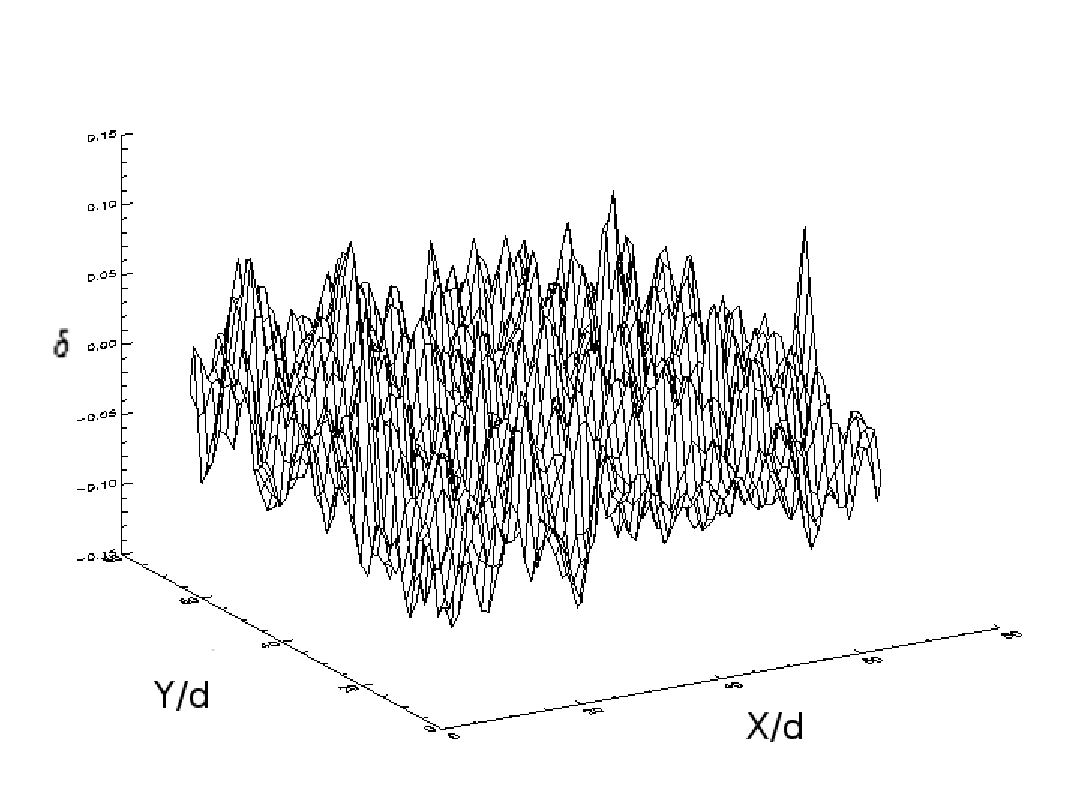
\includegraphics[width=0.49\columnwidth]{./fpa_cos/Delta-0000}
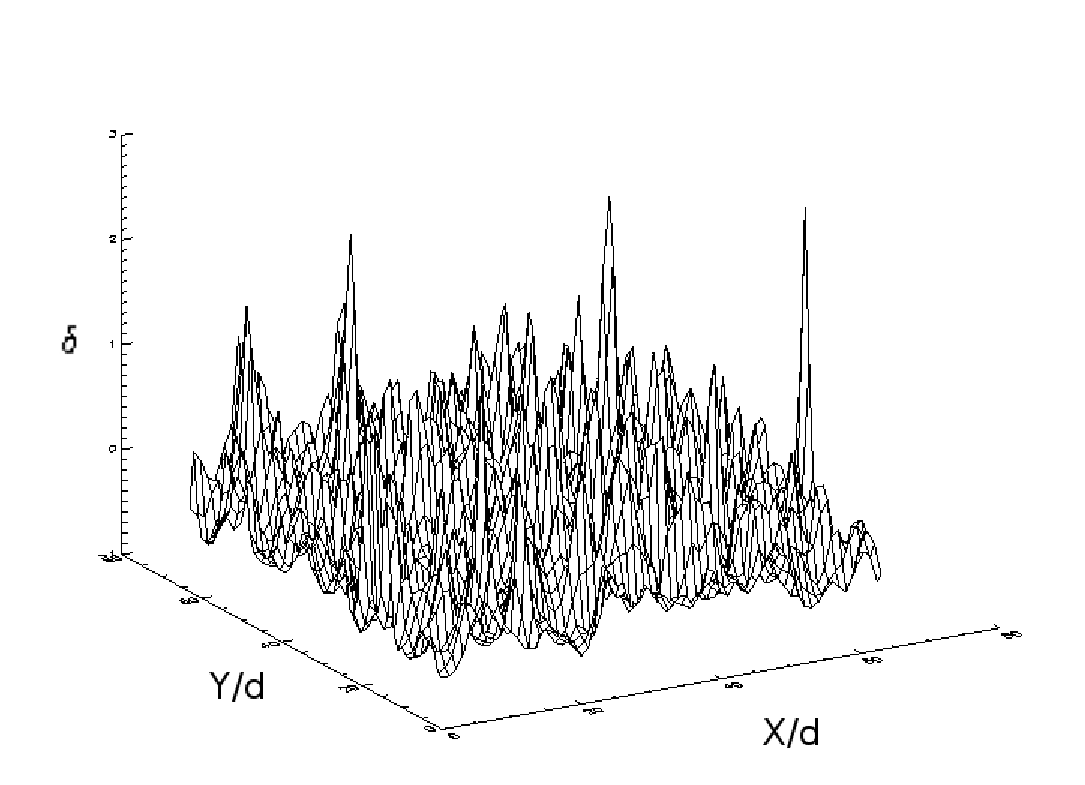
\includegraphics[width=0.49\columnwidth]{./fpa_cos/Delta-0162}
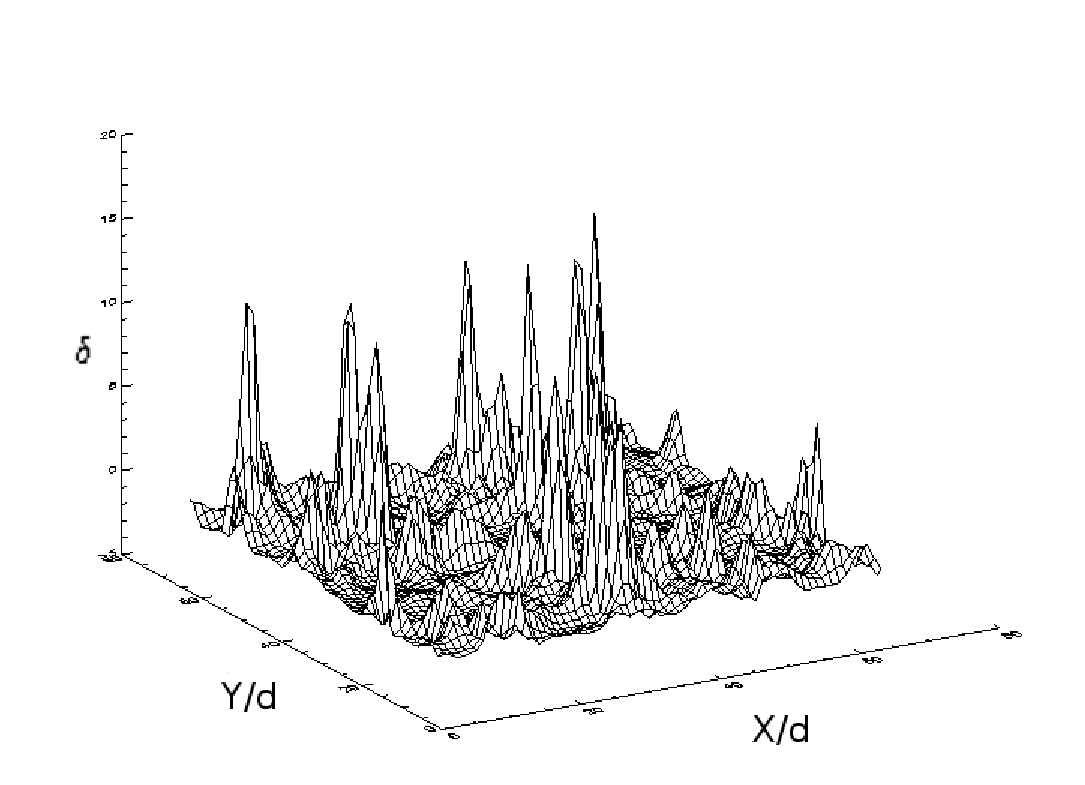
\includegraphics[width=0.49\columnwidth]{./fpa_cos/Delta-0531}
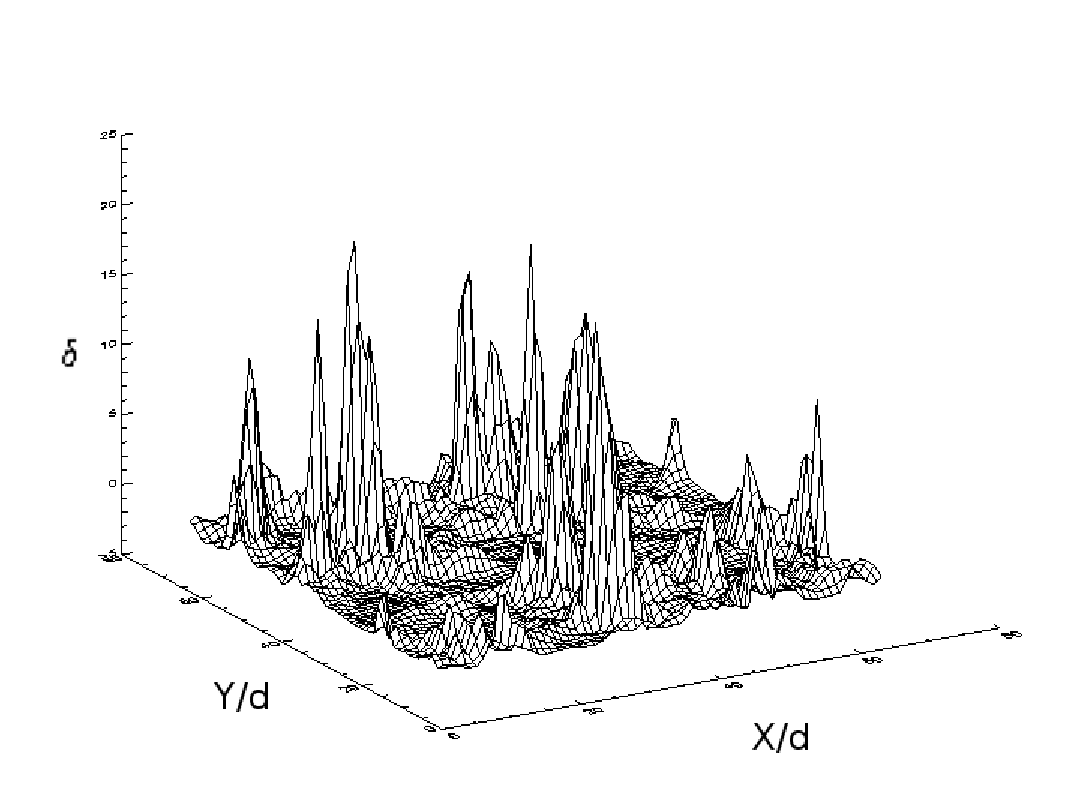
\includegraphics[width=0.49\columnwidth]{./fpa_cos/Delta-0739}
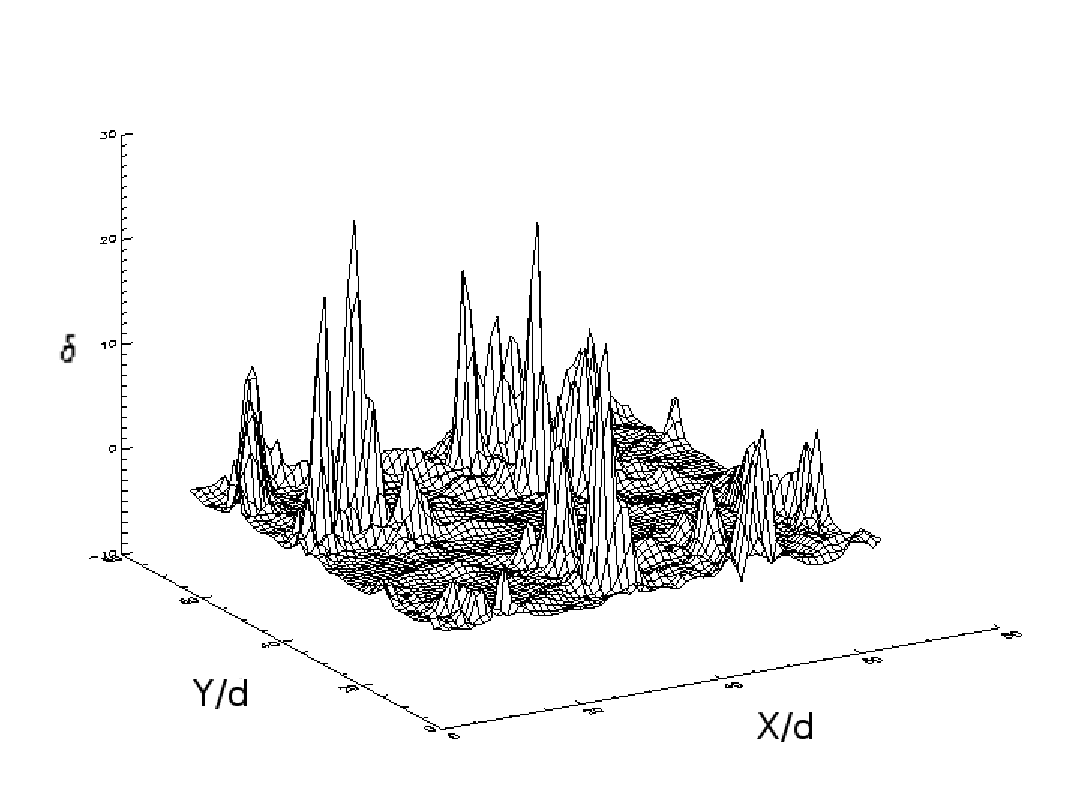
\includegraphics[width=0.49\columnwidth]{./fpa_cos/Delta-0936}

   \end{center}
\caption{The plots here show the evolution of dimensionless density contrast $\delta$ from the 3D FPA code. The $x$ and $y$ axis show dimensionless lengths $x/d$ and $y/d$ as with previous FPA outputs. The output times are $D = 1, 15, 25, 30, 34$. As the simulation evolves we can see structure forming due to gravitational collapse.}
\label{fig.fpa3d}
\end{figure}

\begin{figure}[htb]
   \begin{center}
     %\leavevmode
\includegraphics[width=0.49\columnwidth]{./fpa_cos/hydra/D1001-0162_dc}
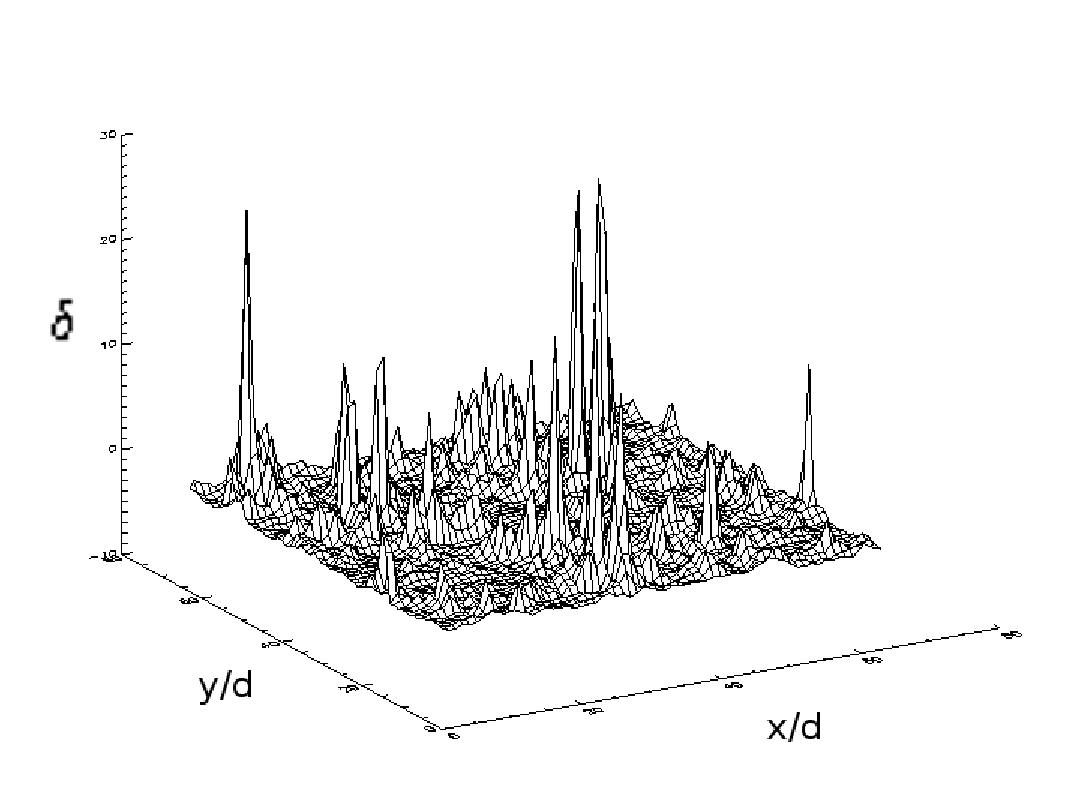
\includegraphics[width=0.49\columnwidth]{./fpa_cos/hydra/D1001-0531_dc}
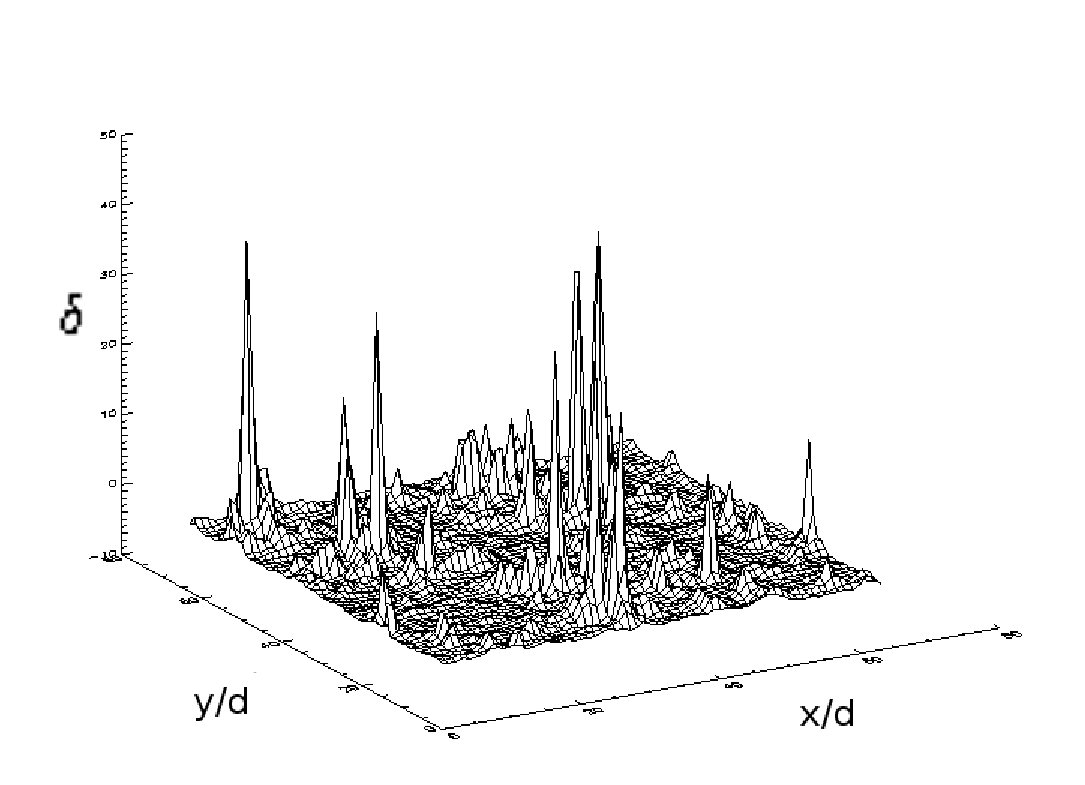
\includegraphics[width=0.49\columnwidth]{./fpa_cos/hydra/D1001-0739_dc}
\includegraphics[width=0.49\columnwidth]{./fpa_cos/hydra/D1001-0936_dc}

   \end{center}
\caption{The plots here show the evolution of density contrast from the Hydra code. The output times correspond to those in the FPA code, they are at timesteps : $t = 162, 531, 739, 936$. Note that the initial density contrast for the two codes is exactly the same hence a plot for timestep 0 ($D=1$) has been omitted from this figure.}
\label{fig.hydra3d}
\end{figure}

\begin{figure}[htb]
   \begin{center}
     %\leavevmode
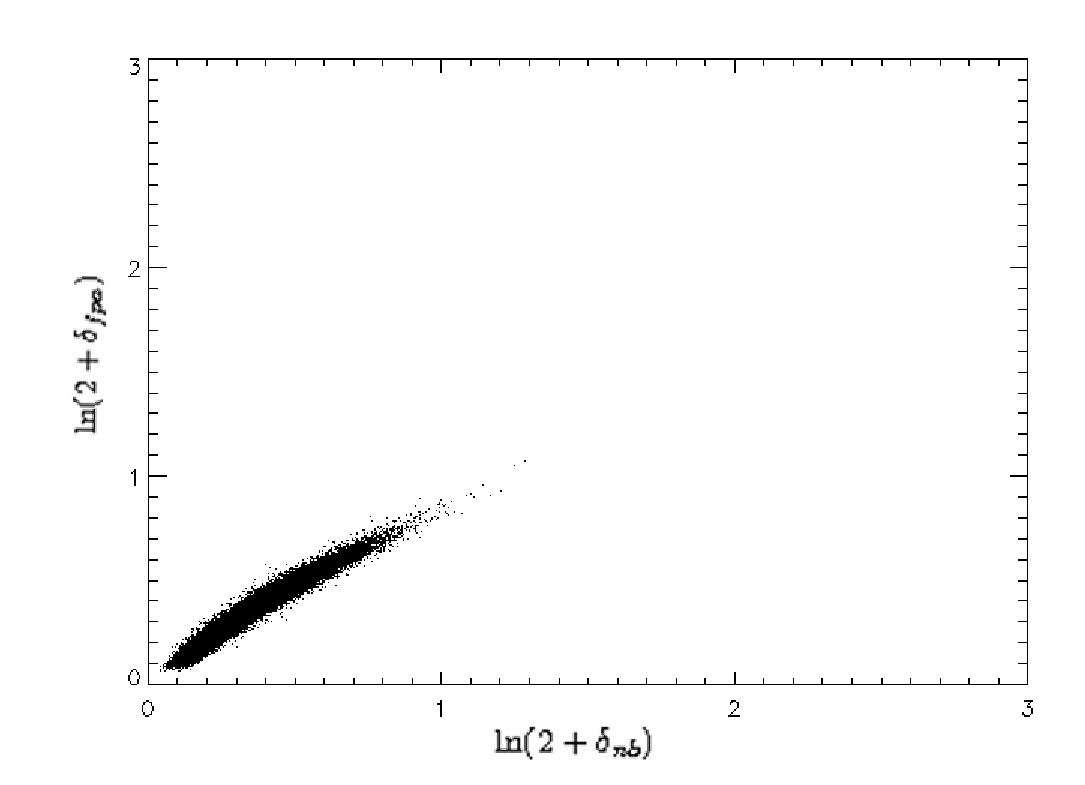
\includegraphics[width=0.49\columnwidth]{./fpa_cos/Lnd_comp_D15_0162_r0-9795}
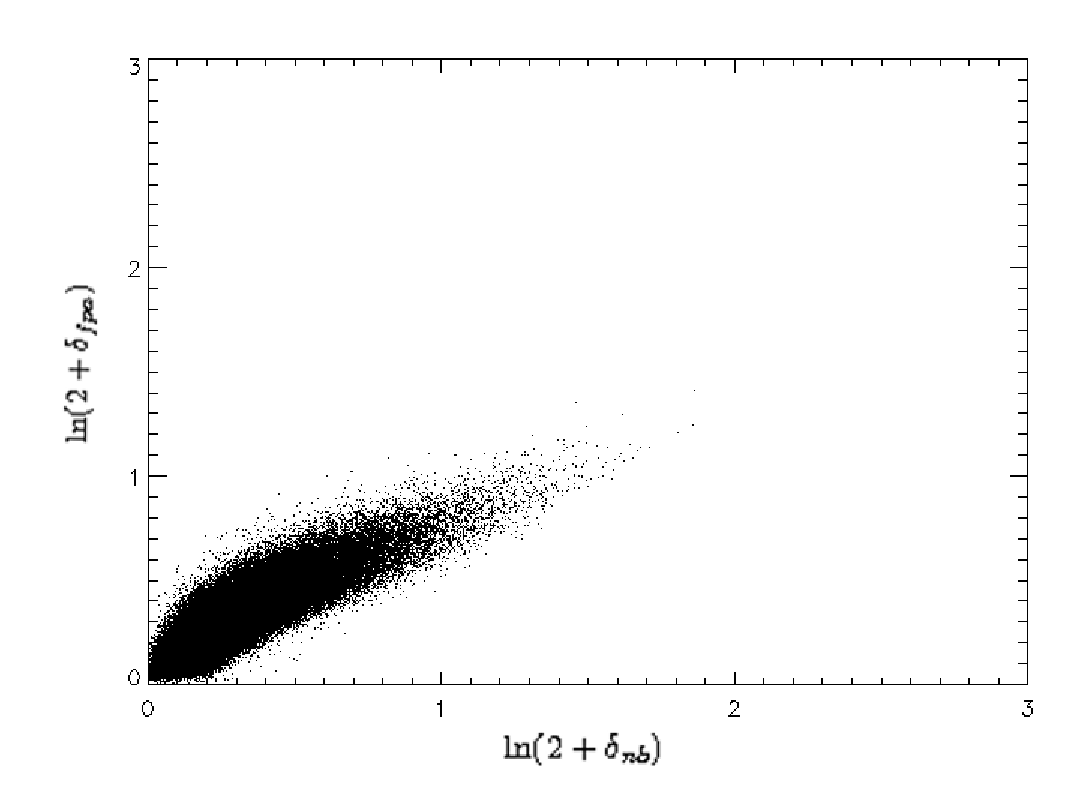
\includegraphics[width=0.49\columnwidth]{./fpa_cos/Lnd_comp_D25_0531_r0-8336}
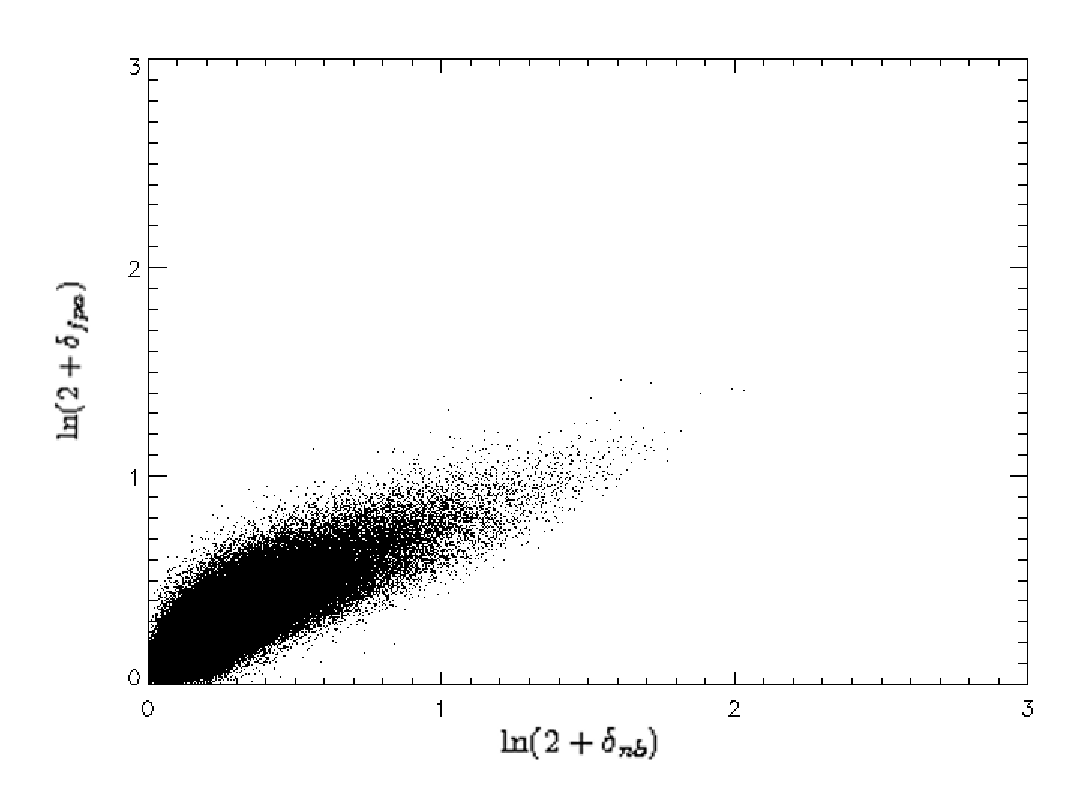
\includegraphics[width=0.49\columnwidth]{./fpa_cos/Lnd_comp_D30_0739_r0-7871}
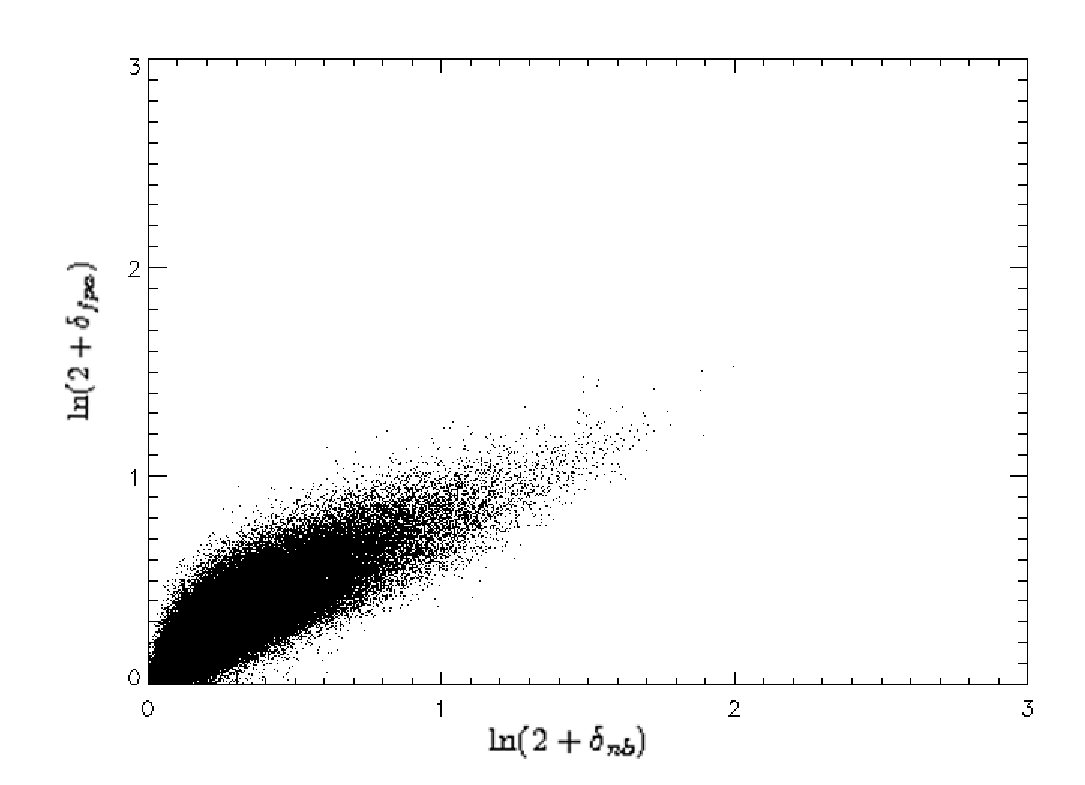
\includegraphics[width=0.49\columnwidth]{./fpa_cos/Lnd_comp_D34_0936_r0-8109}

   \end{center}
\caption{These plots show the correlation between the density contrasts of the $N$-body code (Hydra) and the 3D FPA code. There is a one-to-one correspondence of points from each code, the outputs were matched at the same redshift (that is, time). The x-axis is $\ln(2+ \delta_{nb})$ for Hydra, while the y-axis is  $\ln(2+ \delta_{FPA})$. The correlation coefficients are $r = 0.9795,0.8336, 0.7871, 0.8109$.}
\label{fig.fpacor}
\end{figure}



\subsection{Consistency checks}
As a further test of robustness, we performed a series of checks upon the initial conditions to see if they are consistent with theory. So far we treated the initial conditions generator from Hydra as a black box. We put in cosmological parameters and obtain positions and velocities of the particles (the positions are later turned into density for the FPA code); however, we can examine how well these quantities fit with theory. We expect the histogram of density (and density contrast) to obey a gaussian distribution; although I expect this to be true it is more reliable to check it than just assume it is true. After applying the TSC routine to the positions, we then created a histogram of (over) density and found as gaussian distribution as expected. This is shown in figure \ref{fig.hy_gauss}. Further evidence of this is given by a plot of $\mathcal{I}(\psi) \;{\rm vs}\; \mathcal{R}(\psi)$, as will be shown later in figure \ref{fig.psi_psi}.

We also performed a check of the velocity components which we also expect to be gaussian distributed for each component $x,y,z$. The results of this are shown in the tables below and in figure \ref{fig.hy_vel}. We created histograms for each velocity component and found them to be gaussian, each graph shows an overplot of a theoretical gaussian. The generated velocities are not perfect gaussians but close enough for our purposes. The absolute velocity is shown in the bottom right plot of this figure and it closely follows a Maxwellian distribution as expected. This last plot shows a tighter fit to the underlying theoretical distribution than each of the component velocities. In the tables that follow we tabulate the key parameters of each velocity component.

\vspace*{1cm}
\begin{center}
\begin{tabular}{|r|l|}
  \hline
  quantity & value (km/s) \\ \hline
  max($V_{x}$)  & 169.92818 \\
  min($V_{x}$)  & -184.58659  \\
  mean($V_{x}$) & $9.51\times10^{-9}$ \\
  $\sigma_{v_x}$ & 43.513917 \\
  \hline
\end{tabular}
\end{center}

\begin{center}
\begin{tabular}{|r|l|}
  \hline
  quantity & value (km/s) \\ \hline
  max($V_{y}$)  & 190.18232 \\
  min($V_{y}$)  & -181.42162 \\
  mean($V_{y}$) & $2.888\times10^{-11}$ \\
  $\sigma_{v_y}$ & 43.513917 \\
  \hline
\end{tabular}
\end{center}

\begin{center}
\begin{tabular}{|r|l|}
  \hline
  quantity & value (km/s) \\ \hline
  max($V_{z}$)  & 176.98939 \\
  min($V_{z}$)  & -179.60949 \\
  mean($V_{z}$) & $-2.71\times10^{-9}$ \\
  $\sigma_{v_z}$ & 43.513916 \\
  \hline
\end{tabular}
\end{center}
\vspace*{1cm}

While the maximum and minimum values of velocity are not exactly the same, the width of the three distributions is very similar. The difference only appears in the 6th decimal place. All of the components have mean velocities zero (within machine precision) which denotes that the particles are not experiencing a net bulk motion in some direction. The slight skewing of the distributions is a cause of some concern but the overall behaviour of the simulations are at least believable, hence we do not suspect that something is terribly wrong.

\begin{figure}[htb]
   \begin{center}
     %\leavevmode
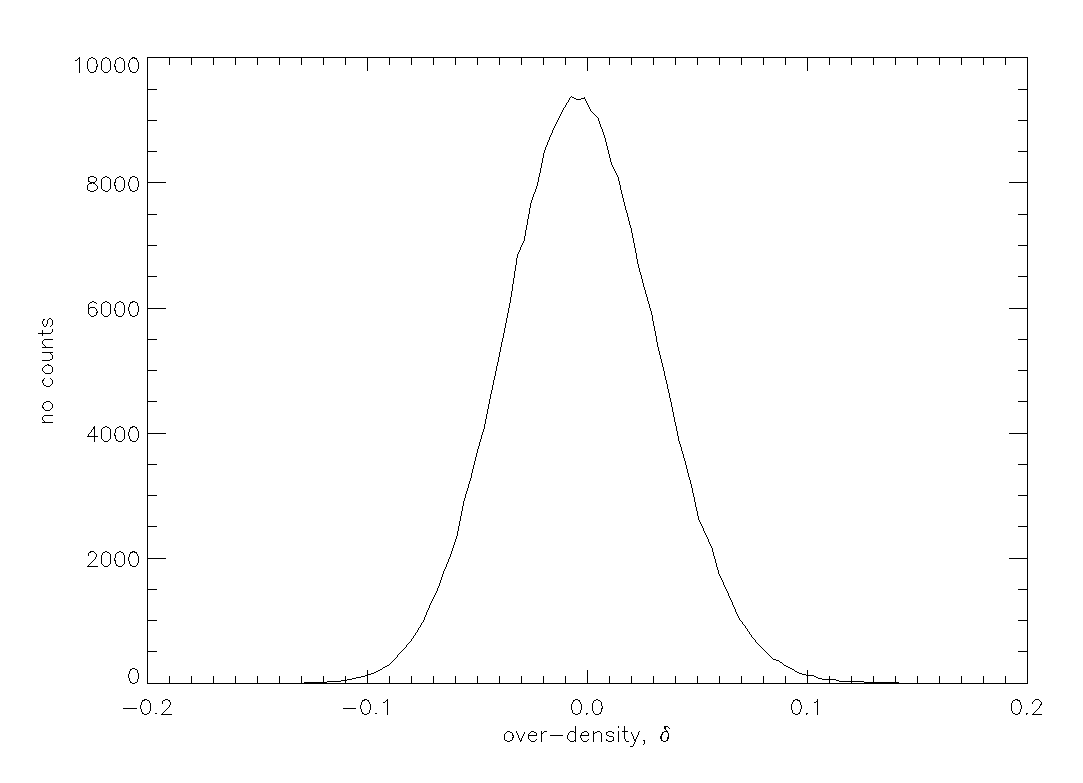
\includegraphics[width=0.49\columnwidth]{./fpa_cos/dc_hist}

   \end{center}
\caption{This plot shows a histogram of density at the start of the simulation. It fits well to a gaussian distribution as expected from theory.}
\label{fig.hy_gauss}
\end{figure}

\begin{figure}[htb]
   \begin{center}
     %\leavevmode
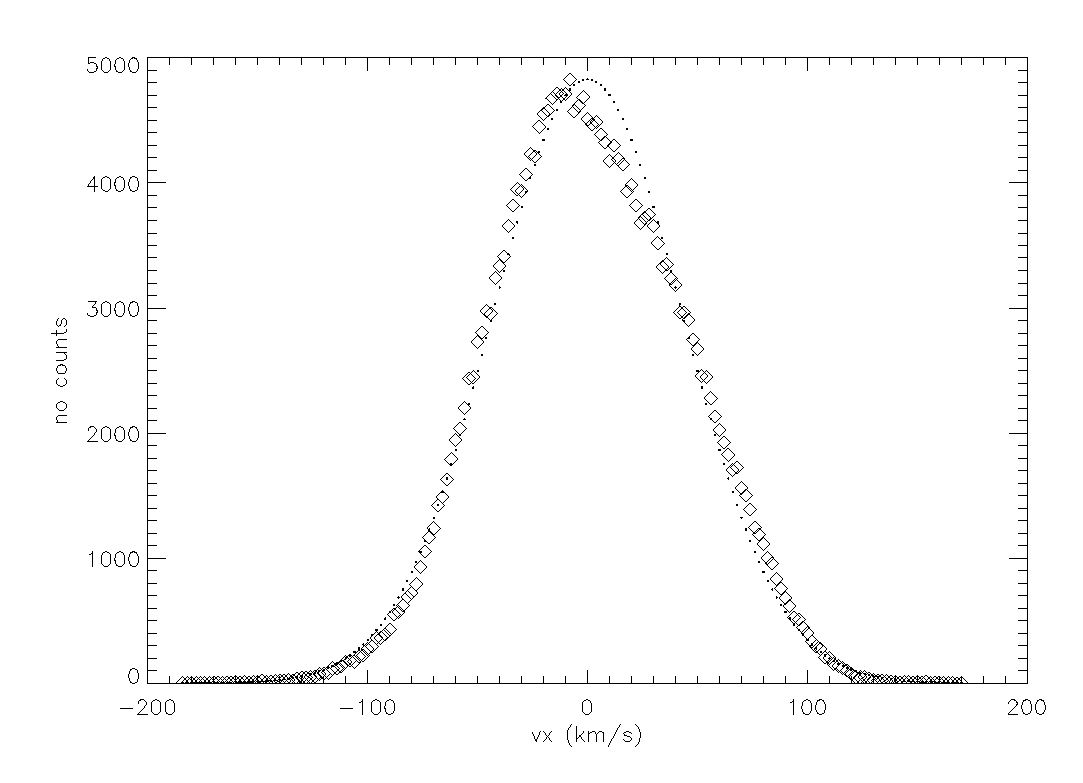
\includegraphics[width=0.49\columnwidth]{./fpa_cos/vel/vx_h_hist}
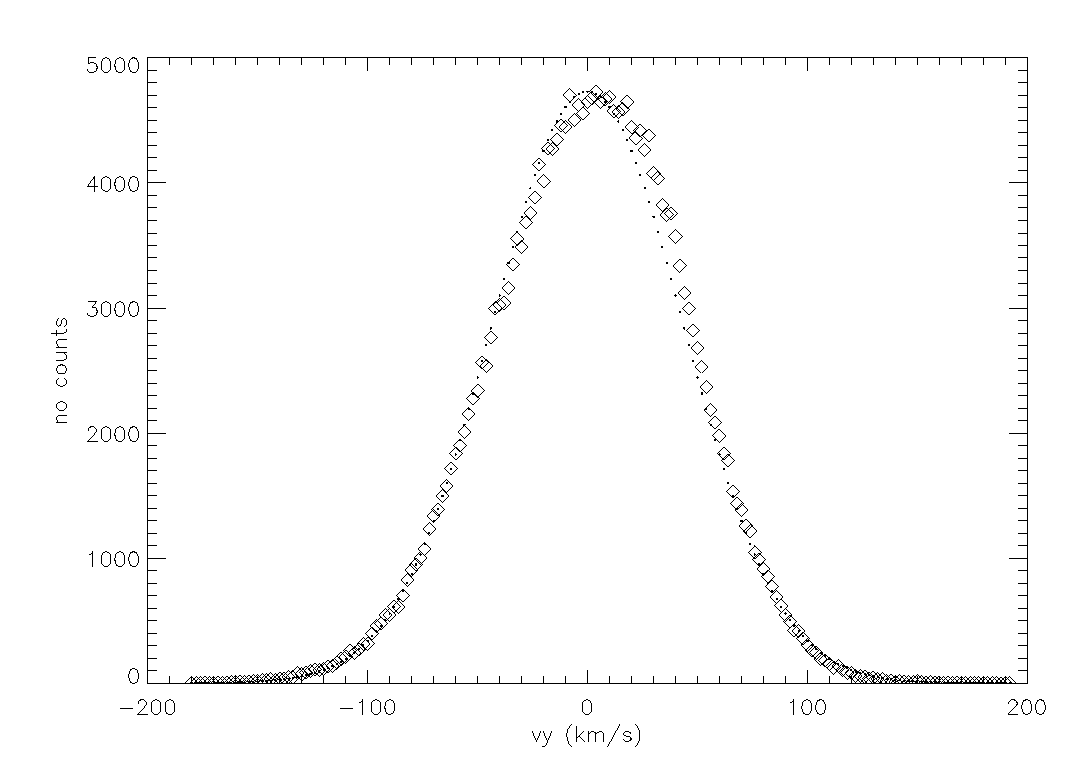
\includegraphics[width=0.49\columnwidth]{./fpa_cos/vel/vy_h_hist}
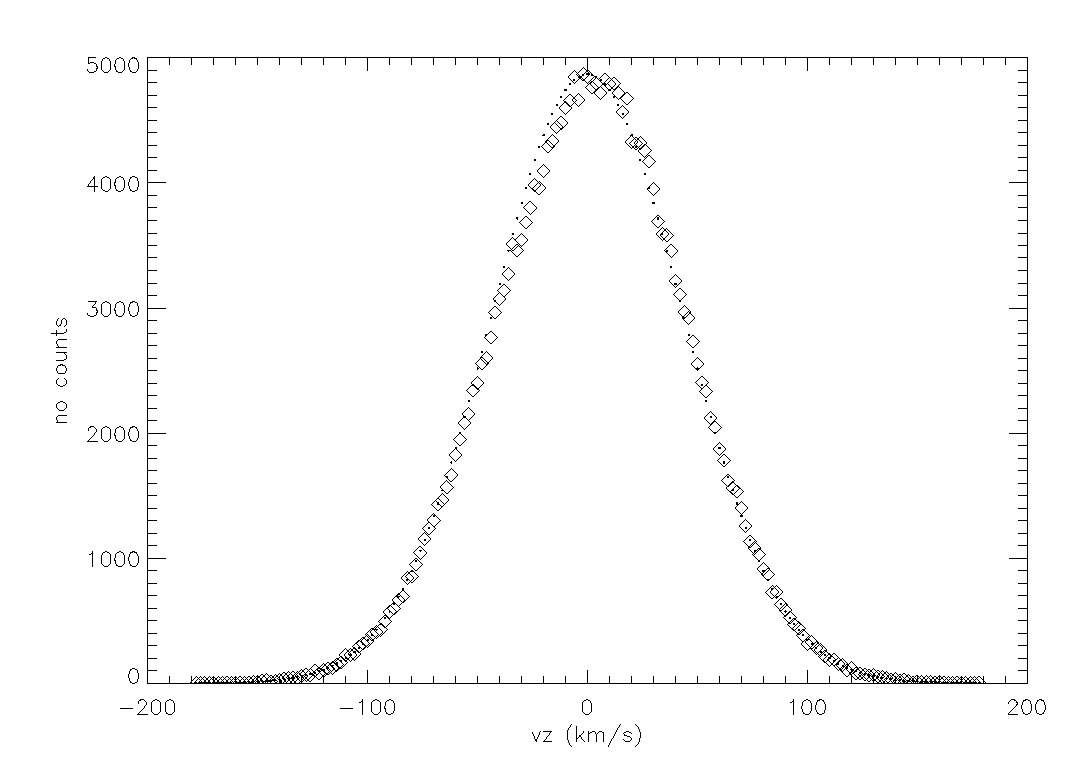
\includegraphics[width=0.49\columnwidth]{./fpa_cos/vel/vz_h_hist}
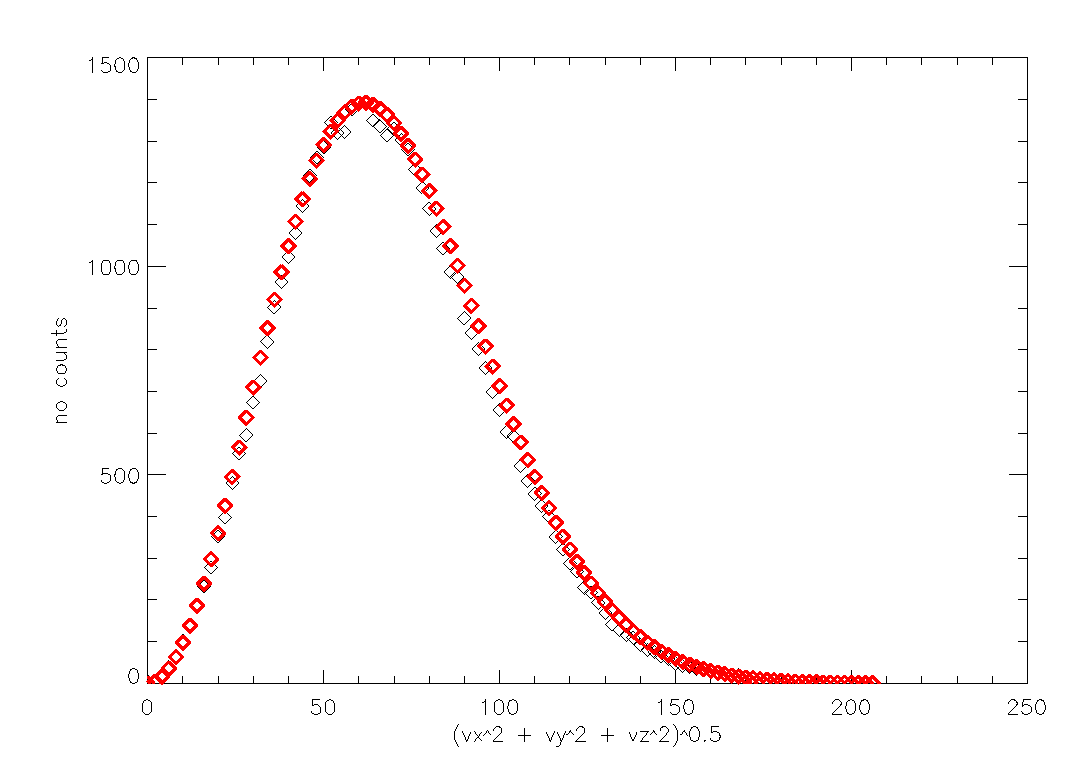
\includegraphics[width=0.49\columnwidth]{./fpa_cos/vel/abs_hist}

   \end{center}
\caption{The plots here show $v_x, v_y, v_z, (v_x^2 + v_y^2 + v_z^2)^{1/2}$ (left-right, top-bottom). The velocity components have a theoretical gaussian overplotted upon them to show how far they deviate from theory. The last plot is overplotted with a theoretical Maxwellian curve which shows a tight comparison between the generated velocity distribution and the expected distribution from theory.}
\label{fig.hy_vel}
\end{figure}

An interesting artefact of wave-mechanics is the apparent deformation of velocities when constructing the wavefunction. From the FPA code, we constructed the velocity field from the probability current (equation \ref{eqn_j}) and then plotted the output against that from the $N$-body code. Figure \ref{fig.hy_fpa_vel} shows a simple point-by-point comparison of the $v_x$ components from the two codes.

\begin{figure}[htb]
   \begin{center}
     %\leavevmode
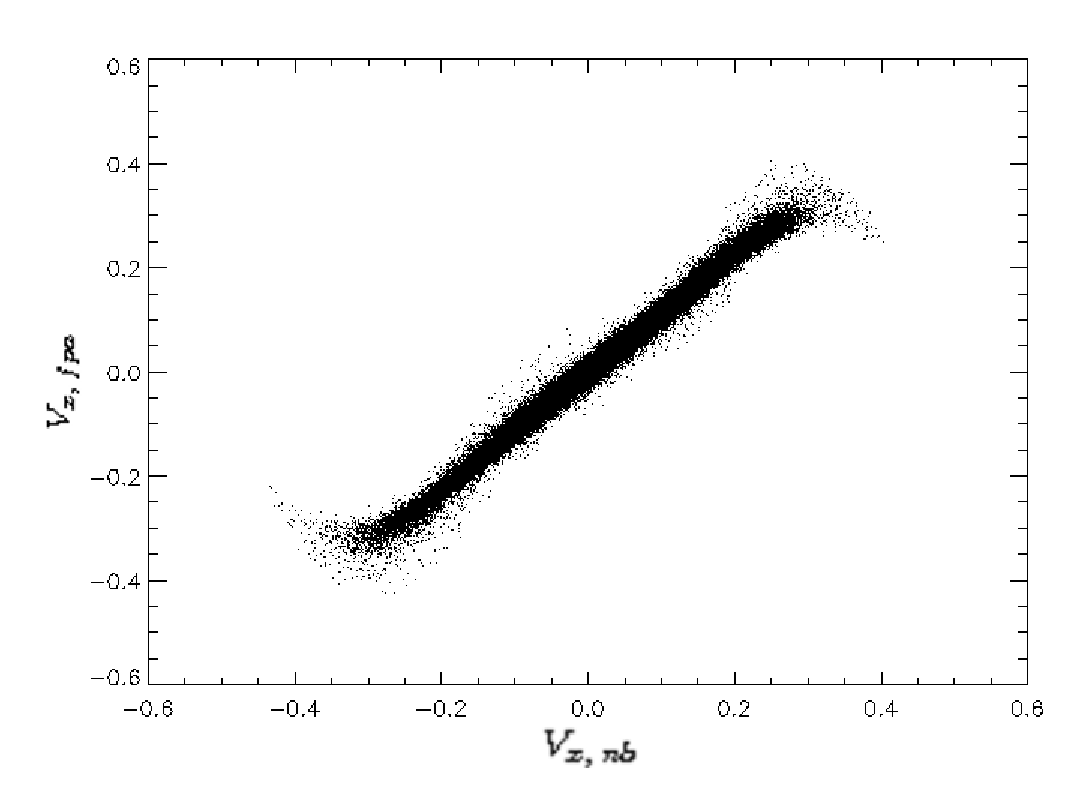
\includegraphics[width=0.49\columnwidth]{./fpa_cos/vel/Vx_comp_1}

   \end{center}
\caption{This plot shows the $v_x$ components from $N$-body along the x-axis and the FPA along the y-axis in the initial conditions. We expected a tight straight line. The turn-over at each end is unexpected and is an artefact from the construction of the wavefunction.}

\label{fig.hy_fpa_vel}
\end{figure}


\subsection{Vorticity}
\label{ch4vort}
In section \ref{vort} we mentioned the possibility of detecting vorticity in our velocity outputs. From theory we do not expect vorticity to exist, hence the presences of vortices in our results may indicate when the code has reached the end of its reliability. As previously mentioned, we expect to find the centre of a vortex at a gridpoint where the velocity is undefined. That is when $v = \nabla\phi$ no longer makes sense. This occurs most obviously when $\psi = (0,0), \;\psi\in\mathbb{C}$ which corresponds to a region of no density: that is a vortical void. Such a region is easy to find computationally. For illustrative purposes I will present graphs of $\mathcal{I}(\psi) \;{\rm vs}\; \mathcal{R}(\psi)$ at 3 different linear growth factors $D = 1, 10, 30$.

At the initial time the distribution of points of the wavefunction corroborate with the fact that the density and velocity follow a gaussian distribution. The circular ring we see has unit radius and the points appear to be even in distribution. At later times the distribution is still evenly distributed (a statement that physics is acting isotropically as required) but the points are no longer a tight ring but smeared out. Eventually the distribution has a closer resemblance to a solid circle. Only at the later times we will see a gridpoint where $\psi = (0,0)$ and hence possibly detect vorticity. From figure \ref{fig.psi_psi} we can see that at $D = 30$ there is potentially a number of gridpoints that are very close to zero.

In figure \ref{fig.vort} we can see an $x-y$ slice at some $z$ of the velocity field. This slice contains a point where the wavefunction is zero. A potential candidate for vorticity. If we look carefully we can see an anomalous velocity vector that has far greater magnitude than the rest of the field. If we zoom into to look closer at this slice then we can see the rest of the velocity vectors `circling' around the wavefunctions null-point.

\begin{figure}[htb]
   \begin{center}
     %\leavevmode
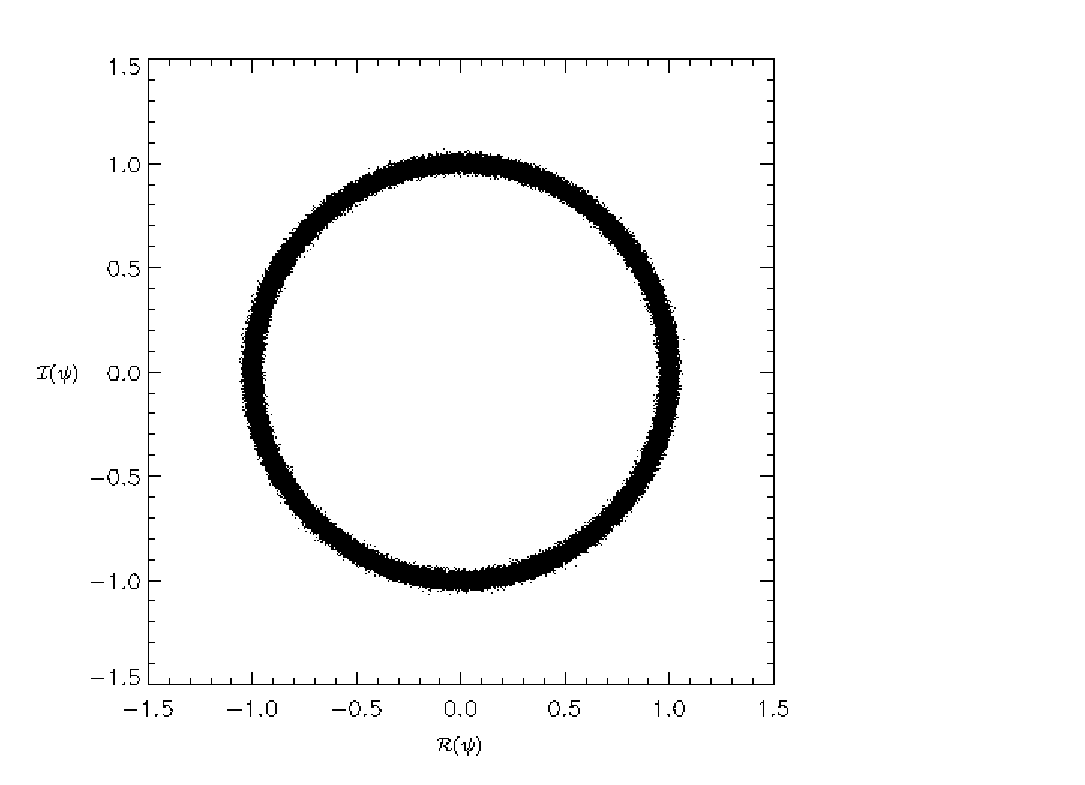
\includegraphics[width=0.49\columnwidth]{./fpa_cos/psi_D1}
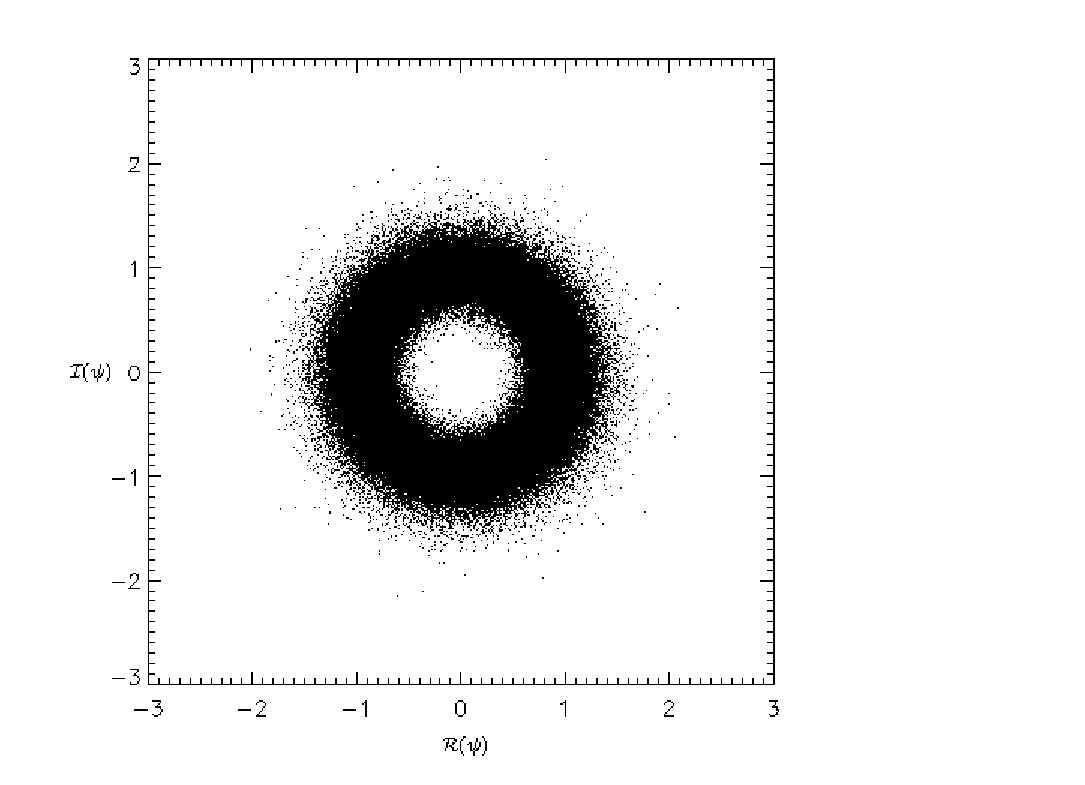
\includegraphics[width=0.49\columnwidth]{./fpa_cos/psi_D10}
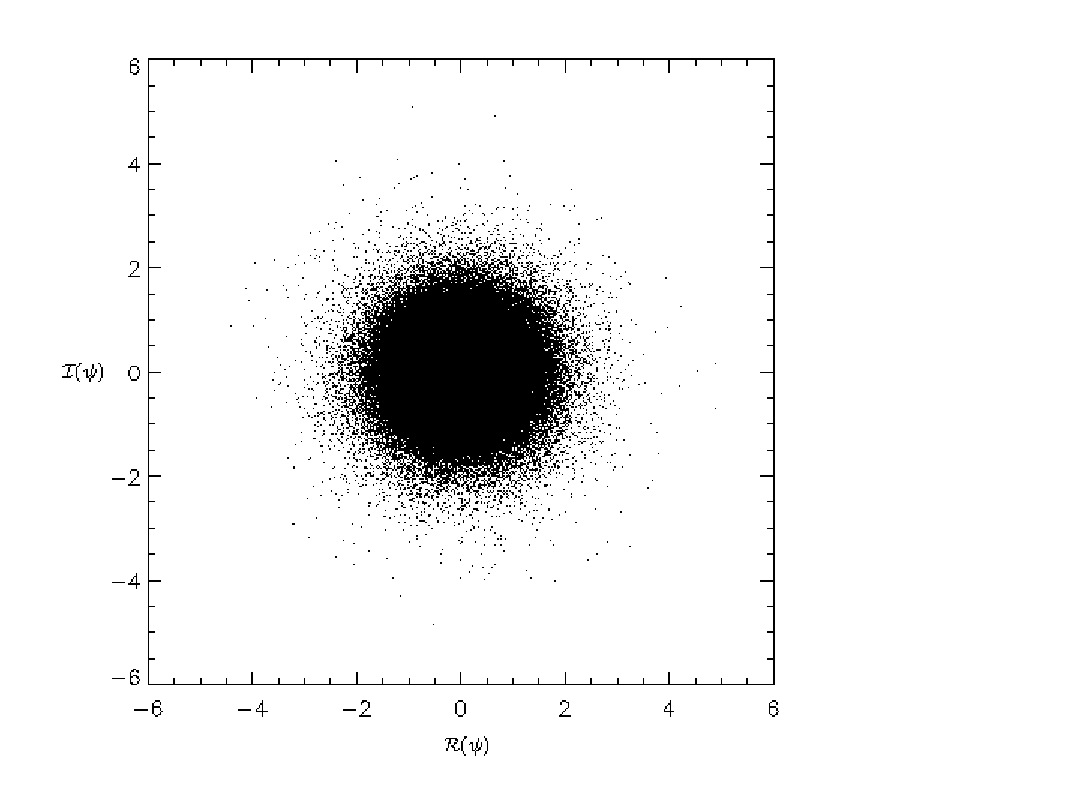
\includegraphics[width=0.49\columnwidth]{./fpa_cos/psi_D30}

   \end{center}
\caption{The plots show $\mathcal{I}(\psi) \;{\rm vs}\; \mathcal{R}(\psi)$ at growth factors $D = 1, 10, 30$. The first plot shows a ring of unit radius as expected from the initial conditions generator. The smearing out of this ring is indicative that the wavefunction is evolving and hence the over-densities are spread further from the mean.}
\label{fig.psi_psi}
\end{figure}


\begin{figure}[htb]
   \begin{center}
     %\leavevmode
\includegraphics[width=0.49\columnwidth]{./fpa_cos/vel/Vel_field}
\includegraphics[width=0.49\columnwidth]{./fpa_cos/vel/Vel_field_zoom}

   \end{center}
\caption{The left plot shows a slice of $x$ and $y$ components of the velocity at time $D = 30$ (showing array element on each axes). On the right is a plot that zooms in, and centres, upon the gridpoint where the velocity vector is largest.}
\label{fig.vort}
\end{figure}


%
%  Conclusion of FPA
%
\section{Conclusion and evaluation of FPA}
The FPA is a fast and efficient method for probing the quasi-linear regime of density perturbations, it proves to be a good match for the Zel'dovich approximation but breaks down at shell crossing as the Zel'dovich method does. The 1D and 3D toy models were a demonstration of the mathematics providing a consistent framework that is able to be coded in such way that gravity (from the Poisson equation) can be coupled to the Schr\"odinger equation.

After testing the toy models, I have confirmed that the FPA can handle `real' cosmological initial conditions and provide simulation results that are comparable to the widely available $N$-body codes (at least in the quasi-linear regime). The benefit of the FPA is that it runs much faster than all known $N$-body codes.

\subsection{From FPA to solving the full system}
To plan our subsequent work it is useful to consider the weaker points of the FPA, such as the inability of the FPA to probe far beyond the linear regime. Like the Zel'dovich approximation it breaks down at high densities. In the dense regions where shell crossing occurs, singularities in density prevent the code from being reliable after shell crossing. The evolution, essentially, becomes `stuck' and does not progress after such a time. This can be circumvented by solving the full Schr\"odinger-Poisson system which allows for multi-streaming (density peaks can pass through one another).

As an extension to the FPA, Short tried a perturbative approach as presented in Chapter 5 of his thesis. This involved adding a perturbation term to the free particle Hamiltonian. The effective potential is still set to zero, so this approach will only allow for small deviations from the kinetic energy term of the free particle Hamiltonian. This approach is still valid in the FPA frame work, hence the code can still jump to any time step. Including the potential term in the Hamiltonian is a non-perturbative approach and is consequently much slower as each intermediate time step has to be calculated. In the next Chapter I present my solution to tackling the full Schr\"odinger-Poisson system.



%
%%
%%%
%%%%
%%%%%
%%%%%%
\newpage
\chapter{Solving the full Schr\"odinger-Poisson system}
\label{ch_5}
% Cayley - unitarity
% Crank-nicolson - Goldberg paper
% Watanabe paper
% need periodicity, unitarity, symplection, expansion
% show 1D solution, extention to 3D, periodicity, gravity)
This chapter provides the main work of this thesis. We consider applying the full Schr\"odinger-Poisson system to the evolution of Large Scale Structure. Any computer code that simulates cosmic structure formation must satisfy some basic requirements in order to provide a fair representation of the Universe. These requirements are:

\begin{enumerate}
\item 3D coordinates;
\item self-consistent gravity; 
\item expanding coordinates;
\item periodic boundaries;
\item mass conserving.
\end{enumerate}

\noindent Hitherto, no published wave-mechanical code seems to meet all of these requirements. The closest publication to meet these requirements is the work of Woo \& Chiueh \citep{bib_wooc}, they seem to have 3D coordinates, self-consistent gravity and expanding coordinates but there is no mention of periodic boundaries or if their code conserves mass. In this thesis we provide full transparency of our method and show how a future researcher could implement their own version of a wave-mechanics code and compare it with our results. The five requirements above are ones that we feel are necessary for all wave-mechanical LSS codes.

In addition to the basic requirements of a generic cosmological code there are a few specific requirements of a code that solves the Schr\"odinger equation, which are unique to this formalism and do not feature in any $N$-body code. This requirements are outlined in the following section \ref{spec_requirements}; they are fundamental requirements of our equations of interest and include: consideration of non-commutative operators, the expression of a exponential of a matrix, and in our particular case we need to have a fast method for matrix inversion to solve the Cayley exponential. The problem of non-commuting operators is not present in $N$-body codes, we circumvent this problem by using splitting operators which do appear in some $N$-body codes (for example, \citet{bib_spr}).

Here I shall re-iterate the equations of interest:

\begin{equation}
\label{eqn_schroedinger2}
 i\hbar\frac{\partial}{\partial t}\psi(\underline{x},t) = \left( -\frac{\hbar^2}{2m} \nabla^2 + mV \right) \psi(\underline{x},t)
\end{equation}

\begin{equation}
\label{eqn_poi2}
\nabla^2 V(\underline{x},t) = 4\pi G \psi\psi^*
\end{equation}

\noindent The potential term $V$ of the Schr\"odinger equation is found by solving the Poisson equation \ref{eqn_poi2}, hence the equations are coupled. The wavefunction $\psi$ is a complex scalar field and the combination $\psi\psi^*$ is the density $\rho$.

The coupled Schr\"odinger-Poisson (S-P) method overcomes many limitations of the FPA but also presents new challenges. The solution to the Schr\"odinger equation is an exponential containing the Hamiltonian operator. Manipulating an exponential that contains a non-diagonal matrix requires careful consideration. Complication is further added by the non-commutativity of the operators. Any computational implementation of the equations should preserve the unitary nature of quantum mechanics and hence be symplectic. As previously mentioned there are many different methods for solving the Schr\"odinger equation and there seems to be no general consensus as to which approach is best. A non-exhaustive list of possible methods follows:

\begin{enumerate}
\item Cayley method;
\item Alternating-Direction Implicit (ADI);
\item Visscher scheme;
\item Chebyshev polynomials;
\item Density Functional Theory.
\end{enumerate}

\noindent I decided to use the same method as Widrow \& Kaiser, which is a finite difference scheme based upon using Cayley's decomposition of an exponential (colloquially called the Cayley method).

\section{Specific requirements of a Schr\"odinger solver}
\label{spec_requirements}
The first concern of solving the Schr\"odinger equation requires thought of how to deal with the exponential term. The main problems are dealing with the exponential of a matrix and the non-commutativity of the operators. I shall highlight each problem in turn.

The solution to the Schr\"odinger equation is given by:

\begin{equation}
 \psi(x, t+dt) = e^{(-iHdt)} \psi(x, t) = e^{(-i(K+V)dt)} \psi(x, t)
\end{equation}

\noindent The operators $K$ and $V$ are represented as matrices. Operating upon these matrices requires extra care. The exponential of a matrix is not the same as a matrix of exponentials. The diagonal matrix is a special case where one can simply exponentiate all the elements along the diagonal. The kinetic energy operator can be expressed as a band diagonal matrix if we use a simple centred difference differentiation method; however, the potential energy term will contain off diagonal elements.

To deal with the matrix exponential, one must use a Lie map to expand the exponential as a power series:

\begin{equation}
 e^{(M)} = \sum_{n = 0} \frac{M^n}{n!} = 1 + M + \frac{M^2}{2!} + \ldots
\end{equation}

\noindent This essentially states that the Taylor series for a matrix has the same form as that for a scalar. There are two useful theorems from Cayley that are relevant to this work. The first theorem is called the Cayley-Hamilton theorem that states that a matrix satisfies its own characteristic polynomial. This provides an expression for matrix inversion (for an $n\times n$ matrix). Matrix inversion is important because we will write the evolution of the wavefunction in such a way that we will require the inversion of the evolution matrix. The extra complication ensures unitarity at the stage of computation, while the evolution as given by a single exponential does not preserve unitarity in computer code \citep{bib_nr}.

\begin{equation}
 e^{(i\frac{1}{2}Hdt)} \psi(x, t+dt) = e^{(-i\frac{1}{2}Hdt)} \psi(x, t)
\end{equation}

\noindent hence, we need to find the evolved wavefunction by inversion as follows:

\begin{equation}
\psi(x, t+dt) =  (e^{(i\frac{1}{2}Hdt)})^{-1} e^{(-i\frac{1}{2}Hdt)} \psi(x, t)
\end{equation}

\noindent Here the power $-1$ that is attached to the first exponential denotes matrix inversion. So we will re-write the exponential using the Lie map but find a formula for invertibility from Cayley.

The second useful theorem from Cayley is that skew-symmetric matrices map to rotation matrices (known as the Cayley transform). For any orthogonal matrix, $A$, we can write:

\begin{equation}
A = (I + M)(I - M)^{-1}
\end{equation}

\noindent provided A does not have an eigenvalue of $-1$ and we require that $(I - M)$ is invertible. The matrix $M$ is a skew-symmetric matrix ($M^T = -M$), and by definition $A^T A = I$. Technically, what is shown here applies to real matrices; however, it also holds true for complex matrices when we substitute skew-symmetric by skew-Hermitian, and orthogonal by unitary. Unsurprisingly, we should note that the space for skew-Hermitian matrices forms the Lie algebra $u(n)$ of the Lie group $U(n)$.

Now we will write our evolution equation as the exponential of a matrix (to first order) using Cayley's transform:

\begin{equation}
 (e^{(-M)})^{-1} e^{(M)} = (1 + M)(1 - M)^{-1}
\end{equation}

\noindent The order of the terms on the right hand side does not matter, as the ``top'' and ``bottom'' brackets commute with each other.

%(Figure out how to put these together. Lie map to linear order looks similar to Cayley transform. Also need to note how to use Cayley transform to turn a continuous problem into a discrete one --- see paper). Approximation works for small dt - remember what tobia said about it spinors being aligned and under the approximation of small rotations (see Noether?)

It is clear that there is a deep connection between the notion of exponential matrices being generators for rotation groups as shown by Lie and the exponential of the Hamiltonian being expressed as a ``rotation'' matrix as given by the Cayley transform. We refer the reader back to Noether's
theorem (see section \ref{sec.sym}) that states that all continuous (or rotational) symmetries of a system provide laws of conservation.

\paragraph{Non-commutative operators}
The final complication comes from the fact that the operators within the exponential are non-commutative. In 1D this is not a problem but becomes a significant problem in higher dimensions. The explicit problem is due to the nature of quantum mechanics where the momentum and position operators do not commute.

\begin{equation}
 [x,p] = xp - px = i\hbar
\end{equation}

\noindent In turn, this means that the kinetic energy (function of momentum) and potential energy (function of position) operators do not commute.

\begin{equation}
e^{K}e^{V}   \ne  e^{V}e^{K} 
\end{equation}

\noindent So it would be wrong to evolve the wavefunction in such a way that two operators (say $\hat{P}$ and $\hat{X}$) were assumed to commute.

\begin{equation}
\hat{P} \hat{X} \psi \ne \hat{X} \hat{P} \psi
\end{equation}

\noindent These operators are assumed to be right associative and are multiplied using the usual matrix product. The problem arises due to the fact that the evolution of a 3D wavefunction requires each dimension to be treated independently. For example, the kinetic energy operator must deal first with the direction $x$ then the direction $y$. For a free particle then the problem of commutativity disappears as each dimension of the momentum operator commutes with itself. When a potential term is added then it is tempting to proceed with computing each dimension independently via the simple 1D Goldberg scheme:

\begin{equation}
\psi(t+dt) = [e^{(-i(K_x + V_x)dt)}  [e^{(-i(K_y + V_y)dt)}  [e^{(-i(K_z + V_z)dt)}\psi(t)]]]
\end{equation}

\noindent However, the Goldberg scheme does not solve the problem of commutativity. Hence it breaks the unitarity evolution of quantum mechanics, and so the evolution of the Schr\"odinger equation is no longer unitary and would not (exactly) conserve mass. To counter the problem of commutativity, Watanabe suggests the use of splitting operators as devised by Suzuki \citep{bib_suz}. The splitting operator technique is a fractal decomposition of exponential operators which provides a robust solution that does not break unitarity. In the main results of this thesis I show that unitarity is well preserved as the mass is conserved (see figure \ref{fig.conserve}), hence the splitting operators fulfil their required role.

\begin{equation}
 e^{(a(P + X))} = [S_m(a/n)]^n + \mathcal{O}(a^{m+1/n^m})
\end{equation}

\noindent Note: many authors call these splitting operators by different names, using any combination of Trotter-Suzuki-Lie. For this work we will stick with calling them (Suzuki) splitting operators. The simplest decomposition is first order in $a$ and is given by:
\begin{equation}
 e^{(a(P + X))} \approx f_1(P,X) = e^{aP}e^{aX}
\end{equation}

\noindent The second order decomposition is given by:
\begin{equation}
 f_2(P,X) = S(a) + \mathcal{O}(a^3) = e^{(a/2)P}e^{aX}e^{(a/2)P}
\end{equation}

\noindent The computational implementation of splitting operators is outlined later in this chapter (section \ref{split}). The problem of non-commutativity does not disappear but the use of splitting operators provide a better way of dealing with the operators. Watanabe notes that energy is no longer exactly conserved but does not appear to blow up either, it is oscillatory around its initial value. Suzuki mentioned in his paper that he aims to construct his splitting operators in such a way that the higher order terms may vanish. As there appears to be no method that can simultaneously deal with all dimensions and not break the rules of commutativity, Suzuki's suggestion is adopted as the best solution.

\section{Numerical method for solving the Schr\"odinger equation}
By now we have a clear idea of how to solve the Schr\"odinger equation; we are following the procedure as suggested by Widrow \& Kaiser. They  used a method that is given in a paper by Goldberg et al \citep{bib_gold} which uses the Cayley transform. Goldberg only considers a 1D system, while Widrow \& Kaiser explored a 2D system -- although it is not clear how they dealt with the problem of commutativity. To expand the Goldberg method to higher dimensions requires a modification via splitting operators. This idea is first presented in the work by Watanabe and Tsukada \citep{bib_wat}.

The two methods of Goldberg and Watanabe are very similar in that both use the Cayley transform. The Goldberg paper provides a clearer outline for solving the equation but some of the subtleties are omitted and the extension to higher dimensions is missing. Watanabe, however, provided a method for extending the Cayley method to higher dimensions in his original paper. \citep{bib_wat}

At the heart of the numerical solution is Cayley's unitary time transformation. Here we are approximating exponentials to first order. The time evolution of a wavefunction using the Cayley transform is:
\begin{equation}
\label{cayley_eqn}
\psi(x, t+dt) = \frac{1- \frac{1}{2} i H dt}{1+ \frac{1}{2} i H dt} \psi(x, t)
\end{equation}

\noindent Numerical Recipes points out that this method is an implicit method similar to Crank-Nicolson \citep{bib_cn}. The Crank-Nicolson method is a 2nd order finite difference scheme that is implicit and unconditionally stable. The scheme employed here is implicit but conditionally stable as it requires a small enough time step. In practice, for particular initial conditions the solver was stable for any choice of $dt$ but this does not appear to be generally true.

\subsection{One dimension}
\label{onedim}
This section outlines the prescription as given in Goldberg. It provides a numerical method for solving the Schr\"odinger equation on a discrete mesh. We wish to see how $\psi$ evolves from time step $n$ to time step $n+1$. For this derivation $\hbar = 1$ and $m = 1/2$. The evolution of the wavefunction can be written as:

\begin{equation}
(1+ \frac{1}{2} i H dt) \;\psi_{j}^{n+1} =  (1- \frac{1}{2} i H dt) \; \psi_{j}^n
\end{equation}

\noindent Or: 
\begin{equation}
\label{cayley_kv}
(1+ \frac{1}{2} i (K+V) dt) \;\psi_{j}^{n+1} =  (1- \frac{1}{2} i (K+V) dt) \; \psi_{j}^n
\end{equation}

\noindent For the kinetic energy term (K), we can write the second derivative, using the centred difference approximation, as:
\begin{equation}
\psi''_{j} = (1/\epsilon^2)(\psi_{j+1} - 2\psi_j + \psi_{j-1}) + \mathcal{O} (\epsilon^3)
\end{equation}

\noindent $\epsilon$ is the grid spacing, $dx$, and $dt$ will be replaced with $\delta$. Inserting the above form of the second derivative into equation \ref{cayley_kv} we get:

\begin{eqnarray}
LHS &=&\psi_j^{n+1} +\frac{i\delta}{2} (\frac{1}{\epsilon^2} (\psi_{j+1}^{n+1} -2\psi_j^{n+1} +\psi_{j-1}^{n+1}) +V^{n+1}\psi_j^{n+1}) \nonumber \\
RHS &=& \psi_j^{n} - \frac{i\delta}{2} ( \frac{1}{\epsilon^2} (\psi_{j+1}^{n} - 2\psi_j^{n} + \psi_{j-1}^{n})  + V^n\psi_{j}^n)
\end{eqnarray}

\noindent After some manipulation this can be written as:
\begin{eqnarray}
\label{evol_psi}
\psi_{j+1}^{n+1} &+& (i\lambda - \epsilon^2 V_{j}^{n+1} -2) \psi_{j}^{n+1} + \psi_{j-1}^{n+1} \nonumber \\
	&=& - \psi_{j+1}^n + (i\lambda + \epsilon^2 V_{j}^n +2) \psi_{j}^n - \psi_{j-1}^n
\end{eqnarray}

\noindent where $\lambda = \frac{2\epsilon^2}{\delta}$. We make an assumption which relates $\psi_{j+1}$ and $\psi_j$. This is the key assumption that enables the system to be solved. Full matrix inversion is far too expensive in terms of computational time. Note that $\psi$ is at the same time on both sides of the equation.

\begin{eqnarray}
\psi_{j+1}^{n+1} = e_j^n \psi_j^{n+1}  + f_j^n
\end{eqnarray}

\noindent where e and f are auxiliary equations. It should be noted that the potential should be given at both the original time and the advanced time in this formulation. However, the advanced potential cannot be known as the system has not evolved. This is a problem for an implicit code. However, under the auxiliary function approximation, we will use the potential at the current time ($n$). This approximation is fine provided the timestep is small enough such that the phase does not evolve too rapidly. The results become unreliable when the latter happens.

This work also differs from Goldberg as a non-static potential was used. Using the assumption given above the evolution is now written as:
\begin{equation}
e_j^n \psi_{j}^{n+1} + f_j^n + (i\lambda - \epsilon^2 V_{j}^{n} -2) \psi_{j}^{n+1} + \psi_{j-1}^{n+1} = \Omega_j^n
\end{equation}

\noindent The function $\Omega$ is introduced here, it is another auxiliary function and is set equal to one side of the evolution equation (compare with equations \ref{cayley_kv} and \ref{evol_psi}). Then we can re-write as:
\begin{equation}
\psi_{j}^{n+1} = (-i\lambda +\epsilon^2 V_{j}^{n} +2 -e^n_j)^{-1} \psi_{j-1}^{n+1} +  (-i\lambda +\epsilon^2 V_{j}^{n} +2 -e^n_j)^{-1} (f_j^n - \Omega_j^n)
\end{equation}

\noindent This provides a formula for the auxiliary functions:
\begin{eqnarray}
e_{j-1}^n &=& (-i\lambda +\epsilon^2 V_{j}^{n} +2 -e^n_j)^{-1} \nonumber \\
f_{j-1}^n &=& e_{j-1}^n (f_j^n - \Omega_j^n)
\end{eqnarray}

\noindent Hence:
\begin{eqnarray}
e_{j}^n &=& 2 -i\lambda +\epsilon^2 V_{j}^{n} - \frac{1}{e_{j-1}^n} \nonumber \\
f_{j}^n &=& \frac{f_{j-1}^n}{e_{j-1}^n} + \Omega_j^n
\end{eqnarray}

\noindent No recursion is needed for $\Omega$:
\begin{equation}
\label{g_omega}
\Omega_j^n = -\psi_{j+1}^{n} + (i\lambda + \epsilon^2 V +2)\psi_{j}^{n} -\psi_{j-1}^{n}
\end{equation}

\noindent These recursion relations are the key equations for solving this system. In Goldberg, destructive boundaries were assumed where the wavefunction disappears at the boundary: ($\psi(L,t) = \psi(0,t) = 0, \; \forall \; t$). To prevent artificial destruction of the wavefunction all simulations by Goldberg kept the wavefunction far from the edges of the system.

As $\psi(0,t) = 0$ (both real and imaginary parts) then we can also assume $e_0 = 0$. Which then gives:

\begin{eqnarray}
e_{1}^n &=& 2 -i\lambda +\epsilon^2 V_{1}^{n} \nonumber \\
f_{1}^n &=& \Omega_1^n
\end{eqnarray}

\noindent As $\psi(L,t) = 0$ then we also have:
\begin{equation}
\psi_{L-1}^{n+1} = -f_{L-1}^n/e_{L-1}^n
\end{equation}

The last formula here provides the expression needed to evaluate the wavefunction at the advanced time. This concludes the method that Goldberg used to solve the 1D Schr\"odinger equation. It is now possible to simulate a simple 1D system, such as reflection from/ and tunnelling through a barrier; these examples were performed during testing as means to checking to see if the code behaved as expected. The results are not directly relevant for a classical simulation and so are omitted for brevity.

Before confronting higher dimensions, and splitting operators, it makes sense to outline how to deal with periodic boundaries and expansion. These features are independent of the use of splitting operators.

\subsection{Periodic boundaries}
\label{per_bound}
In all cosmological simulations, periodic boundaries should be implemented. This ensures that there is no exterior force acting upon the system and hence allows for a statistical way of describing a Universe without end (isotropic and either periodic or extending to infinity). Particles are allowed to cross the boundaries and re-appear on the other side. The exact trajectory of each particle is not important in cosmology, it is more important to analyse the statistical properties (for example, amount of clustering) of the particles at the end of the simulation. Statistically, the amount of clustering in a simulation should be the same as it is in the real Universe.

Considering only 1D for now and instead of assuming $\psi(L,t) = \psi(0,t) = 0, \; \forall \; t$, we will allow the wavefunction to have a non-zero value at the boundary. There is almost no previous work devoted to solving this problem, in all the papers found it seems that only Watanabe has suggested a method for implementing periodic boundary conditions. My attempts to reproduce Watanabe's ``adhesive operators'' \citep{bib_wat} for solving periodic boundaries has been unsuccessful; however, I developed my own method that appears to work well. Unfortunately, it almost doubles the amount of processing required but mass is conserved as required.

Woo \& Chiueh \citep{bib_wooc} consider a fully 3D simulation of Large Scale Structure formation; however, it is not entirely obvious if the boundary conditions are periodic and non-zero. Goldberg \citep{bib_gold} did not consider periodic boundaries and consequently set the wavefunction equal to zero at the boundaries. Watanabe \citep{bib_wat} provides a clear method for implementing non-zero periodic boundaries but he did not apply wave-mechanics to LSS formation.

Our approach is to re-iterate the recursion relations for $e,f$ and $\psi$. From the original method we should notice that $e_0$ is arbitrarily set to zero, this result is used to seed the next value $e_1$. The rest of the function $e$ tends towards some value as it is recursively computed. As the first few values have not converged then there is a discontinuity between the left side ($\psi(x=0)$) and right side of the system ($\psi(x=L)$). Whenever dealing with a system that is far away from the boundaries in the computer then this is not a problem. In some 1D tests I observed that the shape of $e$ looked somewhat similar to that of $V$, which suggests that a discontinuity in $e$ at the boundaries will act like a potential barrier.

This was the key to implementing periodic boundaries: we need to send the wavefunction across the boundary with conserved probability density and without unnatural impedance. These clues point to the natural suggestion of iterating the $e$ function again but instead of assuming that $e_0 = 0$ on the second iteration, I assume that it takes on the value of $e_L$ from the right hand side of the system. That is to say that the function is continuous across the boundary. Doubly iterating $e$ alone isn't enough to ensure periodicity of the system as $f, \Omega$ and $\psi$ also need to be updated ``across'' the boundary.

For the first iteration I will not assume $e_0 = 0$ but rather give it the form that $e_1$ had in the Goldberg paper. This is a simple shift in the recursion relation and is not a problem given that we will re-iterate anyway.

\begin{eqnarray}
e_{0}^n &=& 2 -i\lambda +\epsilon^2 V_{0}^{n} \nonumber \\
e_{1}^n &=& 2 -i\lambda +\epsilon^2 V_{1}^{n} - \frac{1}{e_{0}^n} \nonumber \\
\ldots \nonumber \\
e_{i}^n &=& 2 -i\lambda +\epsilon^2 V_{i}^{n} - \frac{1}{e_{i-1}^n}
\end{eqnarray}

\noindent Then we perform the second $e$ recursion but use the last value of the first recursion to seed the second recursion. So $e_0$ now uses $e_L$:
\begin{eqnarray}
e_{0}^n &=& 2 -i\lambda +\epsilon^2 V_{0}^{n}- \frac{1}{e_{L}^n} \nonumber \\
e_{1}^n &=& 2 -i\lambda +\epsilon^2 V_{1}^{n} - \frac{1}{e_{0}^n} \nonumber \\
\ldots \nonumber \\
e_{i}^n &=& 2 -i\lambda +\epsilon^2 V_{i}^{n} - \frac{1}{e_{i-1}^n}
\end{eqnarray}

\noindent After calculating $e$, we perform the first of the $f$ recursions:
\begin{eqnarray}
f_{0}^n &=&  \Omega_{0}^n \nonumber \\
\ldots \nonumber \\
f_{j}^n &=&  \Omega_{j}^n +  \frac{f_{j-1}^n}{e_{j-1}^n}
\end{eqnarray}

\noindent The second $f$ recursion follows, naturally (using $f_L$ from the first iteration to seed the second iteration):
\begin{eqnarray}
f_{0}^n &=&  \Omega_{0}^n +  \frac{f_{L}^n}{e_{L}^n} \nonumber \\
\ldots \nonumber \\
f_{j}^n &=&  \Omega_{j}^n +  \frac{f_{j-1}^n}{e_{j-1}^n}
\end{eqnarray}

\noindent Lastly, we perform the recurrence relation for $\psi$, which recurs (backwards) from $L$ to $0$ rather than the other way round. The following relations are performed twice to correctly calculate $\psi$ in the same way that $e$ and $f$ are doubly recursed. The values of $\Omega$, however, do not need to be performed twice as they do not involve recursion.

\begin{eqnarray}
\psi_{L}^{n+1} &=&  (\psi_{0}^{n+1} -f_{L}^n)/e_{1}^n \nonumber \\
\ldots \nonumber \\
\psi_{L-1}^{n+1} &=& (\psi_{L}^{n+1} -f_{L-1}^n)/e_{L-1}^n
\end{eqnarray}

In practice we found that the recursion relations only have to be performed twice. The relations have converged by the second iteration so we do not require further recursion. This result will be shown explicitly in section \ref{per_bou}.

\subsection{Expansion}
The evidence for an expanding Universe is well known and is accepted as part of the standard model of cosmology. From a coding point of view, the first consideration is whether to deal with physical density or comoving density. This work follows Widrow \& Kaiser in only considering comoving densities which are, by definition, a conserved quantity. The first model of an expanding Universe that we try is the same one as presented by Widrow \& Kaiser: the Einstein de Sitter model. Then we go on to provide more general equations that can model all flat FLRW Universes.

\subsubsection{Einstein de Sitter model}
The latter part of the Widrow \& Kaiser paper deals with a particular Cosmological scenario: the Einstein de Sitter model. This model is a flat, matter only Universe (curvature parameter $k = 0$ and $\Omega = \Omega_m = 1$). Note that $\Omega$ here is the density parameter from Cosmology and not the $\Omega$ as it appears in the Goldberg method above in equation \ref{g_omega}.

We take the usual S-P system but re-write the equations using expanding coordinates:

\begin{eqnarray}
 i \hbar \frac{\partial}{\partial t} \psi &=& \left(\frac{-\hbar^2}{2 m a^2} \nabla^2 +mV\right) \psi \\
 \nabla^2 V &=&  \frac{4\pi G}{a} (\psi\psi^* - <\psi \psi^*>)
\end{eqnarray}

\noindent We perform the following transformations into dimensionless quantities:

\begin{eqnarray}
\chi &=& \psi (6 \pi G t_0^2 )^{1/2} \\
y &=& x/L \\
U &=& 3 t_0^2 a V / 2L^2
\end{eqnarray}

\noindent $L$ is the physical length of the system, in our final results we use $ L = 500$ Mpc. Here $a$ is the scale factor between the physical position $r$ to the comoving position $x$, $r = a x$. The Einstein-de-Sitter Universe has an analytic form for the expansion scale factor $a = (t/t_0)^{2/3}$. The usual condition for the present day scale factor is: $a(t_0) = 1$.

In studying the methodology of Widrow \& Kaiser we identified a significant typographical error and an apparent inconsistency in the definitions presented in their paper. In the interests of pedagogy and clarity it is instructive to explain thoroughly the logical steps that led us to this conclusion.

In the Widrow \& Kaiser paper they suggest tracking the physical density rather than the comoving density:  $<\psi \psi^*>  = \rho a^3 = \rho_{crit}$. The critical density $\rho_{crit}$ of the Universe is the density require to make the Universe have a flat geometry. We assumed this statement to be true and then implemented their suggested equations in a code but found that the density was conserved (physical density should decrease as the Universe expands). This prompted further investigation into the equations and assumptions presented in their paper. We found that from the definition of the wavefunction, and from the definition of the transforms presented, that the density must be comoving and hence a conserved quantity.

Initially we wondered if $\psi$ was physical but $\chi$ is comoving; however, we soon found that this cannot be the case. The suggested scaling relation between the two variables does not account for expansion, the proportionality between the two quantities is a fixed constant. This means that both are physical or both are comoving. In the Schr\"odinger equation the scaling factor that transforms $\psi$ to $\chi$ drops out, which means that this factor could be arbitrary. This means that the two quantities could be either physical or comoving and the Schr\"odinger equation would be the same in either case. This was unexpected as we expected a transformation from physical to comoving (or vice-versa) to affect the dynamics. Resolution to this conundrum is found in the Poisson equation; we found that there is an extra factor of $a$ left over from such a transformation.

Here we will show that the wavefunction represents a comoving density. If we start from the assumption that density is physical ($<\psi \psi^*>= \rho a^3 = \rho_{crit}$), as Widrow \& Kaiser did, then we see the following:

\begin{eqnarray}
<\psi \psi^*> &=& \rho_{com} a^3 = \rho_{crit} = \frac{3 H^2}{8\pi G} \\
	 &=& \frac{1}{6\pi G t^2} \\
<\chi \chi^*> &=& \frac{6\pi G t_0^2}{6\pi G t^2}
\end{eqnarray}

\noindent If the density is comoving then: $<\psi \psi^*>= \rho_{com} = \rho_{crit} a^3 $. This gives the following expression for $<\chi \chi^*>$:

\begin{eqnarray}
<\psi \psi^*> &=& \rho_{com} = \rho_{crit} a^3 = \frac{3 H^2 a^3}{8\pi G} \\
	 &=& \frac{a^3}{6\pi G t^2} = \frac{t^2}{6\pi G t^2 t_0^2} = \frac{1}{6\pi G t_0^2} \\
<\chi \chi^*> &=& \frac{6\pi G t_0^2}{6\pi G t_0^2} = 1
\end{eqnarray}

\noindent Here we can see that the expression for $<\chi \chi^*>$ is a fixed constant over time, hence the latter version of $<\chi \chi^*>$ represents a comoving rather than a physical density. We believe that our result is consistent with the original transformation $\chi = \psi (6 \pi G t_0^2 )^{1/2}$; hence $<\psi \psi^*> = \frac{1}{6\pi G t_0^2}$ and $<\chi \chi^*> = 1$ are comoving quantities.

Equation (17) of Widrow \& Kaiser has a typographical error, the coupled equations erroneously appear as one equation. The derivation of those equations is in Appendix \ref{app_eds}, here I provide them as they should have appeared:

\begin{eqnarray}
i \frac{4\mathcal{L}}{3} \frac{\partial}{\partial \ln a}\chi &=& -\nabla_y^2 \chi + \frac{4\mathcal{L}^2}{3} U \chi \\
\nabla_y^2 U &=& \chi\chi^* - 1
\end{eqnarray}

\noindent here $\mathcal{L} = \frac{m a^{1/2}L^2}{\hbar t_0}$.

These equations are solved in the same manner as before: we use Goldberg's method with a gravitational potential and implement periodic boundary conditions. This new version of the equations will account for the expansion. The evolution of the wavefunction is written as:

\begin{equation}
\chi(x, t+dt) = \exp(-\frac{i 3 H}{4 \mathcal{L}} d \ln a) \chi(x,t)
\end{equation}

\noindent Computationally, this exponential term will be re-expressed using Cayley's transform. The timesteps $dt$ are of equal size such that the time in the computer code is discrete and evenly spaced. The computational time steps represent real (physical) steps in the natural log of the expansion factor, that is $dt = d \ln a$. This means that the timesteps are evenly spaced in $\ln a$ but obviously not so in terms of $a$. Initial conditions for this model are discussed later.

\subsubsection{Flat models with non-zero cosmological constant}
\label{gen_exp}
In this section an algorithm is outlined that describes a flat Universe with non-zero cosmological constant. We assume that the geometry is still flat $k=0$ but the background Universe does not have to be matter dominated ($\Omega =1$ but $\Omega \ne \Omega_m$). We adopted an approach of finding a set of dimensionless variables that create a dimensionless Schr\"odinger equation as Widow \& Kaiser have done but in a way that also accounts for non-zero cosmological constant. The assumption of working with a comoving density is still true: $<\psi \psi^*>= \rho_{com} = \rho_{phys} a^3 $. The further necessary assumptions are:

\begin{eqnarray}
y &=& x/L \nonumber \\
\nabla^2 U &=& \chi \chi^* - 1 \\
\end{eqnarray}

\noindent These assumptions plus the Friedmann equation will lead to the necessary form of the Schr\"odinger equation. The Friedmann equation dictates expansion and hence provides the background cosmological model. However, a simplified form can be written by noting the relation between the density parameters $\Omega$.

\begin{eqnarray}
H^2 &=& H_0^2 [\Omega_{m_0} (1 + z)^3 + (1 - \Omega_{m_0})] \nonumber \\
\Omega_m &=& \frac{\Omega_{m_0}(1 + z)^3}{\Omega_{m_0} (1 + z)^3 + (1 - \Omega_{m_0})}
\end{eqnarray}

\noindent This leads to the simplified form of the Friedmann equation:
\begin{equation}
H^2 \Omega_m a^3 = H_0^2 \Omega_{m_0}
\end{equation}

\noindent Here $H = \dot{a}/a$ is the Hubble parameter (has units that are $1/time$, in this case we used $1/ {\rm years}$). With the two assumptions and the Friedmann relations above then it is possible find the other dimensionless quantities $\chi$ and $U$:

\begin{eqnarray}
\chi &=& \left(\frac{8\pi G}{3 H_0^2 \Omega_{m_0}}\right)^{1/2} \psi \nonumber \\
U &=& \left(\frac{2 a}{3 L^2 H_0^2 \Omega_{m_0}}\right) V
\end{eqnarray}

\noindent These relations are consistent with the desired form of the Poisson equation: $\nabla^2 U = \chi \chi^* - 1$. The corresponding Schr\"odinger equation is:

\begin{equation}
2 i \mathcal{L}\left[\Omega_{m_0} +(1-\Omega_{m_0}) a^3 \right]^{1/2} \frac{\partial\chi}{\partial \ln a} = \left[-\nabla^2 + 3\Omega_{m_0}\mathcal{L}^2 U\right] \chi 
\end{equation}

\noindent Here $\mathcal{L} = \frac{m a^{1/2}L^2 H_0}{\hbar}$. This version of the Schr\"odinger equation will reduce to the Einstein de Sitter version using the appropriate scaling relations in the case where $\Omega_{m_0} = 1$.

\subsection{Higher dimensions}
To implement a Schr\"odinger solver in more than one dimension requires solving the equation for each spatial dimension sequentially.  This is to say that we solve for the $x$ dimension first then the $y$ and $z$ dimensions, one after the other. This poses a problem if the time steps are too large: there must be enough spatial resolution to approximate the correct three dimensional trajectory.

Without the knowledge of using splitting operators it is tempting to try a simple extension to the Goldberg method:

\begin{equation}
\psi(t+dt) = [e^{(-i(K_x + \frac{1}{3}V)dt)}  [e^{(-i(K_y + \frac{1}{3}V)dt)}  [e^{(-i(K_z + \frac{1}{3}V)dt)}\psi(t)]]]
\end{equation}

\noindent The operators are right associative, so the the operator closest to the wavefunction on the right hand side is the first operator to act upon the wavefunction. The newly updated wavefunction is then acted upon by the next closest operator and so on until all three dimensions are done. So far there appears to be no way to combine all three spatial dimensions in one operation. Commutation relations must be observed and unitarity must be preserved in order to ensure energy and mass conservation. Under this method there is a clear problem with energy conservation as $P$ and $V$ do not commute.

\subsubsection{Splitting Operators}
\label{split}
The naive approach of extending the Goldberg method to higher dimensions is not as robust as Watanabe's suggestion to use splitting operators. Here I will present the approach that I adopted, it is one that uses Suzuki's method of operator splitting.

\begin{equation}
\psi(x, t+dt) = e^{-i (K+V) dt} \psi(x, t) = e^{-i K dt/2} e^{-i V dt} e^{-i K dt/2} \psi(x, t)
\end{equation}

\noindent In higher dimensions it is possible to make use of the following commutation relation: $[P_x, P_y] = 0$. Here $P_x$ and $P_y$ are the momentum in the $x$ and $y$ directions. Only considering the kinetic energy would give:

\begin{eqnarray}
 e^{-i(K_x + K_y + K_z)dt} &=& e^{-i K_x dt} e^{-i K_y dt} e^{-i K_z dt} \nonumber \\
\psi(x, t+dt) &=& \frac{1- i\frac{dt}{2} K_x}{1+ i\frac{dt}{2} K_x} \frac{1-i\frac{dt}{2} K_y}{1+i\frac{dt}{2} K_y}\frac{1-i\frac{dt}{2} K_z}{1+i\frac{dt}{2} K_z} \psi(x, t)
\end{eqnarray}

\noindent Updating the wavefunction in this way allows for a modular code. Kinetic energy and potential energy operators can be switched on or off as desired: that is to say that we can easily run our code with the potential energy routine turned `off' by using a simple check flag in our initial conditions. This should allow the code to run quicker than just setting Newton's gravitational constant $G$ to zero.

As a consequence of re-writing our code in such a modular way, the form of $e$ will change as it does not contain the potential term $V$ (confer: equations in section \ref{onedim}). Now it will have a form resembling:
\begin{equation}
e = 2 - i\lambda
\end{equation}

\noindent Here $\lambda = 4\epsilon^2/\delta$. The form for $f$ remains unchanged while the $\Omega$ now has no $V$ term. Updating the wavefunction for the potential is straight forward:

\begin{equation}
e^{-i V dt} \psi(x, t) = (1 -\frac{i\delta}{2}V)(1 +\frac{i\delta}{2}V)^{-1} \psi(x, t)
\end{equation}


% ----------------- End of Schroedinger solving ------------------
\section{Solving the Poisson equation}
\label{sol_poi}
The final piece of coding needed is a method for computing the potential. This term is the `interaction' term in the Schr\"odinger equation, it provides the gravitational interaction between the otherwise free particles. As previously mentioned it is not an interaction term as is used in the quantum mechanics literature. There is no scattering or creation/annihilation: two dense regions of matter will attract towards each other and then pass straight through each other. The Poisson equation for the gravitational potential is equivalent to Newton's equation of gravitational force (a two-point function). The potential field is continuous; however, this method forces softening at scales smaller than the cell length which truncates the gravitational force.

The equation relating potential to density is:
\begin{equation}
 \nabla^2 V =  4\pi G \psi\psi^*
\end{equation}

\noindent To solve for $V$, this can be re-written as:
\begin{equation}
 V =  \int 4\pi G \psi\psi^* dV
\end{equation}

\noindent A possible method for solving this equation would be to replace the nabla operator with an equivalent expression in Fourier space. The $k$ subscripts denotes the Fourier space equivalent version of the variable.
\begin{eqnarray}
k^2 V_k &=&  4\pi G \psi_k \psi_k^* \nonumber \\
V_k &=&  \frac{4\pi G \psi_k \psi_k^*}{k^2}
\end{eqnarray}

\noindent This requires solving the equation in Fourier space. As noted in Numerical Recipes \citep{bib_nr}, when dealing with a finite number of Fourier modes it is possible to improve upon the simple method proposed above of dividing by $k^2$ using cosines:
\begin{eqnarray}
 V_k &=&  \frac{4\pi G \psi_k \psi_k^*}{ 2 \kappa - 3} \nonumber\\
 \kappa &=& (\cos(2 \pi n/L) + \cos(2 \pi m/L) + \cos(2 \pi o/L))
\end{eqnarray}

\noindent $m,n,o$ are indices that enumerate the grid points, they run from 0 to $L-1$.

\section{Computational algorithm}
In this section I will bring together all of the previous ideas in order to outline the flow of computation in my wave-mechanics code.
This algorithm satisfies the five requirements (3D, self-consistent gravity, expansion, periodic boundaries, mass conserving) presented at the start of this chapter. The results section (\ref{ch5_results}) of this chapter will validate this claim.

\begin{enumerate}
\item Construct initial wavefunction
\item Start time loop
\item Perform first split-operator of kinetic energy
\begin{enumerate}
\item calculate auxiliary function $e$
\item calculate $\Omega$
\item calculate auxiliary function $f$
\item update wavefunction
\end{enumerate}
\item Perform potential energy operation
\begin{enumerate}
\item gravitational potential calculated using standard Fourier technique
\item update wavefunction
\end{enumerate}
\item Perform second split-operator of kinetic energy (as before)
\item End time loop
\end{enumerate}


\section{Initial Conditions}
Through out the code testing process the main initial condition used was that of a gaussian density profile. This manifests itself as a gaussian envelope: the real part of the wavefunction.  In some cases it was appropriate to add a velocity component to the wavefunction, an initial `kick', which appears as a carrier wave of the wavefunction. This allowed the code to be tested for a free particle with and without an initial velocity. They were applied in the testing phase of the code in all dimensions (1 to 3). The initial 1D wavefunction is:

\begin{equation}
\psi_i = \frac{1}{(2\pi w^2)^{1/2}} \;  e^ {\left( -\frac{(x_i-x_0)^2}{4 w^2} + i p_0 x_i \right)}
\end{equation}

\noindent Here $p_0$ is the initial momentum, $x_0$ is the offset of the peak from the origin, $x_i$ is the gridpoint at which the function is being evaluated, $w$ is the standard deviation of the gaussian. The pre-factor before the exponential is the usual normalization factor.

In further testing, two or more gaussian density profiles were combined to see the effect of waves passing through each other (both as free waves and as gravitationally interacting waves). The initial wavefunction for two waves starting at points $x_0, x_1$ with initial momenta $p_0, p_1$ and widths $w_0, w_1$ is:

\begin{equation}
\psi_i =  e^{\left( -\frac{(x_i-x_0)^2}{4 w_0^2} + i p_0 x_i + \frac{(x_i-x_1)^2}{4 w_1^2} + i p_1 x_i \right) }
\end{equation}

\noindent the normalization factor has been dropped, it is not necessary to include this as it merely normalizes the total of the wavefunction to 1. This total can be any number that one desires so long as the total is constant for the duration of the simulation.

Another common and useful test of any cosmological code is a tophat collapse. The name of this test takes its name from the shape of the (1D) density profile it has. If we take a Universe which has uniform density everywhere and then create an area of increased density about the origin in a spherically symmetric manner. This should produce a step function in density at the boundary between the uniform density of the Universe and the central area which has an increased amount of density. In one dimension this produces a tophat shape in the density profile (that is, a step at the boundaries on either side of the origin. This is a test that typically uses periodic boundary conditions which ensures that only the central density will collapse while the rest of the Universe (the background) remains static. This is a direct test of Birkhoff's theorem (which is also described in \ref{on_spacetime}).

I performed this test in 3D in order to understand how different choices of parameters affect the system. There are many parameters to consider so searching this parameter space is daunting. Running the tophat tests mainly helped to guide the choice of the $\nu$ parameter to pick when running the code for proper cosmological initial conditions. The results of tophat testing can be found in section \ref{tophat}.

\subsection{Cosmological Initial Conditions}
The main test of my cosmological wave-mechanics code is to compare it with an $N$-body code. The choice of $N$-body code is GADGET-2 \citep{bib_spr}, it is perhaps the most popular code in use today. The $N$-body simulations were performed by Sabiu of UCL. The prescription of comparing these results with my wave-mechanics code will follow the methodology suggested by Short as seen in Chapter \ref{ch_4}. The underlying theory of cosmological initial conditions is provided in Chapter \ref{ch_3}.

The number of mesh points will determine the density (or mass) resolution available, $128^3$ gridpoints is roughly equivalent to $128^3$ super-particles in an $N$-body code. As previously mentioned, the amount of mass per particle in $N$-body code is fixed but in our case the amount of mass per fluid element can change (although the total of the entire box is fixed). In the initial conditions, the mass per fluid element or mass per mesh in our Wave-mechanics code is the same as the mass per particle of an $N$-body code.  It also sets the spatial resolution as we will take some length for our box (say 100 Mpc on the side) and divide it up into $32, 64, 128$ gridpoints (or mesh points) as we require. In this way, the number of mesh points in a Wave-mechanics code sets the density resolution as it sets both spatial and mass resolutions.

Here I will briefly recapitulate the method used in Chapter \ref{ch_4}: we generated a smooth density field from the particle positions in the initial conditions file. Then we constructed the wavefunction from this density field. Finally, we evolved the wave-mechanics code and compared the outputs with those from the Gadget code. The latter code always outputs particles positions which were smoothed to give a density field. The results from the cosmological simulations are presented in section \ref{cos_sim}.

\section{Results}
\label{ch5_results}
In all of the wave-mechanics literature hitherto the codes are presented as mature and fully developed but few details are presented of how such codes were constructed. As this thesis has highlighted, there are many barriers to creating a successful wave-mechanics code. It is not obvious that previous codes overcame such difficulties. Consequently, as a wave-mechanics code requires many components working together then it is necessary to show the pieces working individually in simple scenarios before presenting the full 3D results.

At the heart of the wave-mechanics code presented in this thesis is an extension of the algorithm as presented by Goldberg et al \citep{bib_gold}. Naturally, the first step was to create a one dimensional code that reproduced the results from this publication. For expediency, I do not reproduce these results in this thesis. Their results illustrated a one dimensional wave-packet incident upon different energy barriers. I believe that the results that do appear in this thesis section corroborate with the results of Goldberg. That is to say that the Schr\"odinger equation works as expected.

Presented in this thesis are tests of the periodic boundaries, a three dimensional two-body gravitational interaction and a three dimensional tophat collapse. The first two do not seem to appear in previous literature. Our method for implementing periodic boundaries is entirely new and previously unpublished. Lastly, I will present my results from a full cosmological simulation.

\subsection{Periodic Boundaries}
\label{per_bou}
My first attempt to create periodic boundaries mimicked the work presented in Watanabe \citep{bib_wat}. In that work the method used is called the `adhesive operator' (not to be confused with the Zel'dovich adhesion approximation). Mild success came from adopting this approach, periodicity worked in the simplest tests but mass was not conserved. Hence, the adoption of Watanabe's solution is temporarily rejected on grounds of mass not being conserved. It is a possible direction of future work. It is worth reiterating that the method used by Watanabe is very similar to that of Goldberg. Both methods avoid explicit matrix inversion and make use Cayley's of decomposition of exponentials.

The intrinsic problem of using the Goldberg method is that it requires the wavefunction to be kept far away from the boundaries. The wavefunction is not defined at the boundaries and the method for updating the evolution at every timestep requires the wavefunction to be zero at the boundaries. Simply allowing the wavefunction to be non-zero at the boundaries is not enough. The functions that evolve our system must update across the boundary: that is to say that the left and right side of the system must connect to one another smoothly (without a discontinuity). 

As discussed in section \ref{per_bound}, the evolution functions $e,f,$ and $\Omega$ must smoothly connect across the boundary. We can see from the form of $e$ that it is a recursion relation which converges to some value. We notice that $e_0$ is arbitrarily set to zero and that this result is used to seed the next value $e_1$. This function then tends towards some value for the rest of the gridpoints.

As I will show in figure \ref{fig.test_e}, the function $e$ takes on some of the shape of the potential $V$. This was the crucial breakthrough in understanding why the recursion relations are at the heart of the periodic boundary problem. In the simple 1D tests I noticed that once $e$ has fully converged it resembles the exact shape $V$; however, as the first few values have not converged then there is a discontinuity between the left side ($\psi(x=0)$) and right side of the system ($\psi(x=L)$). This discontinuity will act like a potential barrier.

It was natural to guess that the $e$ function would be free from discontinuities if we iterate through the recursion relation for a second time. In the second iteration, I use the value of $e_L$ from the right hand side of the system to seed the new value for $e_0$ on the left hand side of the system. In practice I found that I also had to doubly iterate the equations for $f, \Omega$ and $\psi$ (to ensure mass conservation).

Figure \ref{fig.test_e} also shows that it is unnecessary to perform a third iteration as the second and third iteration are exactly the same. If the relations had not completely converged by the second iteration then the system would not conserve mass. Furthermore, I provide the caveat that while the graphs for all three iterations look similar there is enough of a difference that the first iteration of $e$ does not allow for complete mass conservation when the wavefunction approaches the edge of the system.

From Watanabe's paper it is not apparent if his solution to periodic boundaries overcomes this problem of recursion; however, the solution he offered is admittedly more elegant if it can be made to work.

\begin{figure}[htb]
   \begin{center}
     %\leavevmode

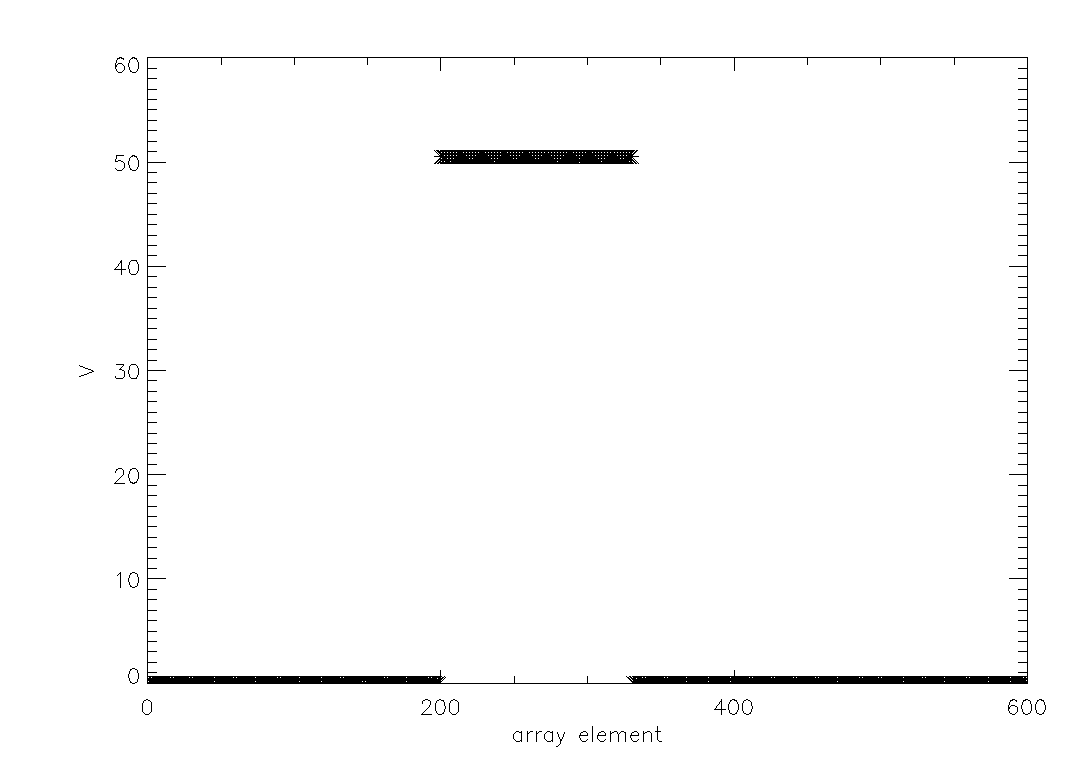
\includegraphics[width=0.49\columnwidth]{./full/test/V}
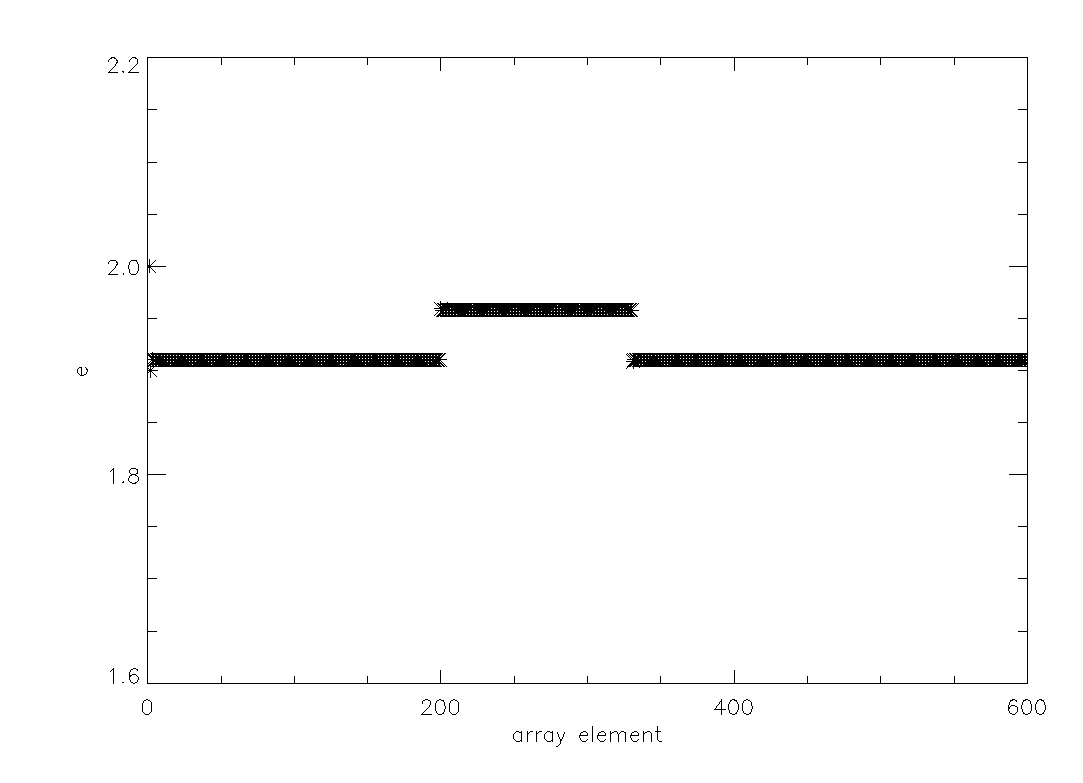
\includegraphics[width=0.49\columnwidth]{./full/test/e}
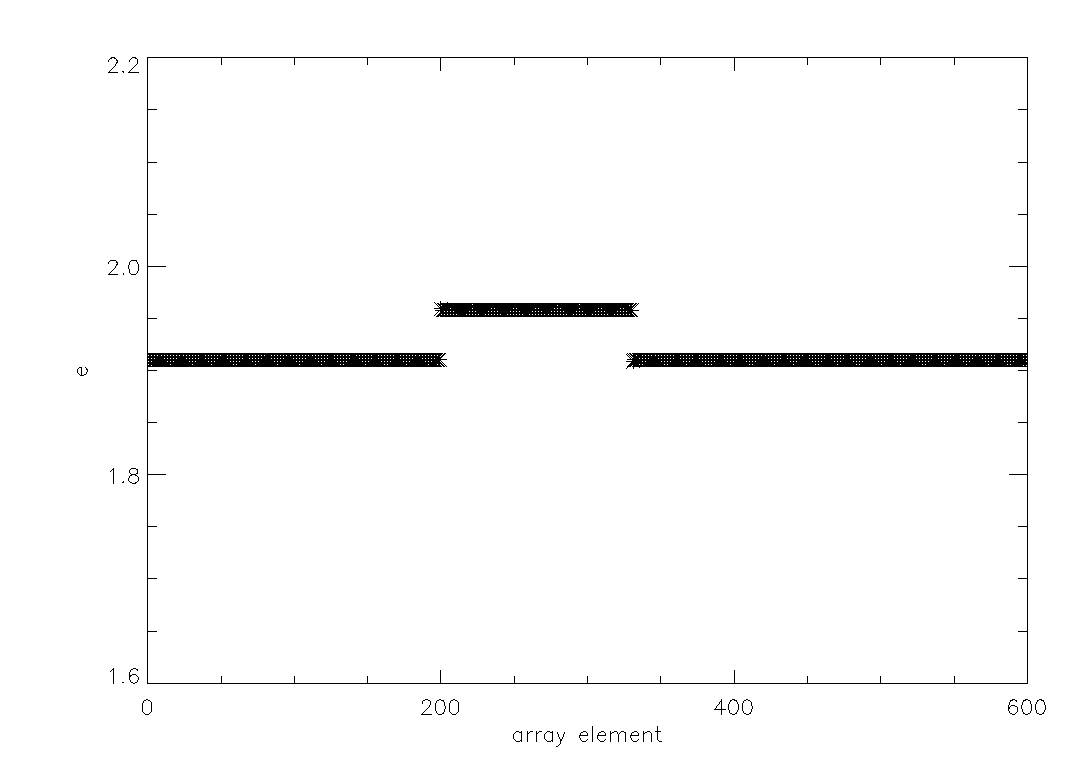
\includegraphics[width=0.49\columnwidth]{./full/test/e2}
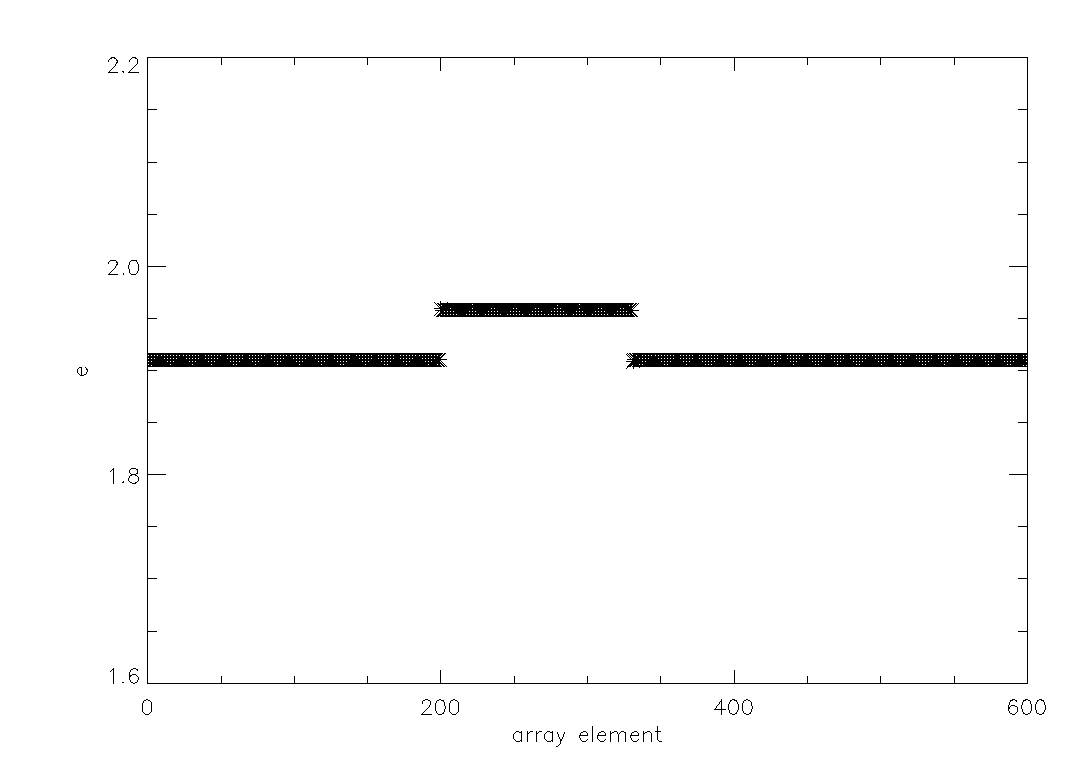
\includegraphics[width=0.49\columnwidth]{./full/test/e3}

   \end{center}
\caption{The plots here show recursion of the $e$ function over first, second and third iteration (top-right, bottom-left, bottom-right). The top-left graph is potential $V$ and is here to show the resemblance between its shape and that of $e$. On the first $e$ iteration we note that there is a `blip' (the start of the recursion relation). The last graph (bottom-right) is a third iteration and shows the same result as the second iteration. Number of gridpoints: $N_g= 600$.}
\label{fig.test_e}
\end{figure}

As corroborative evidence I present the outputs from a 3D simulation; figure \ref{fig.test_bound} shows a 2D slice where the wave-packet (shown as $\psi^*\psi$) passes through all 4 boundaries in the plane. There is no underlying potential well so the wave-packet behaved as a free particle and shows dispersion over time.

\begin{figure}[htb]
   \begin{center}
     %\leavevmode
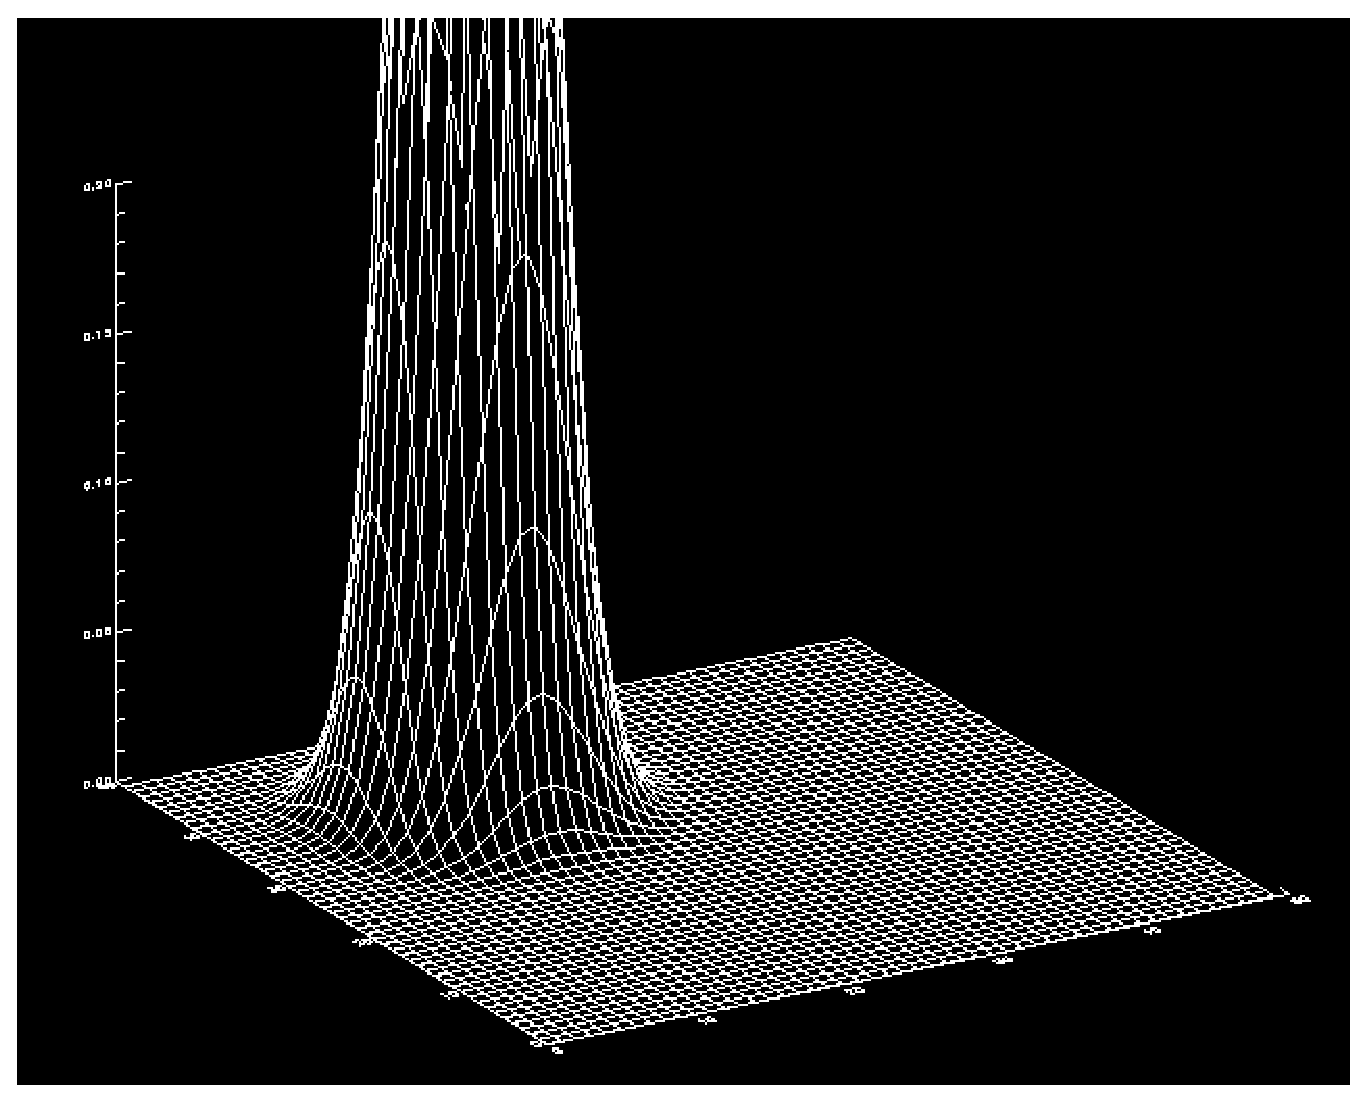
\includegraphics[width=0.49\columnwidth]{./full/test/deltas_00}
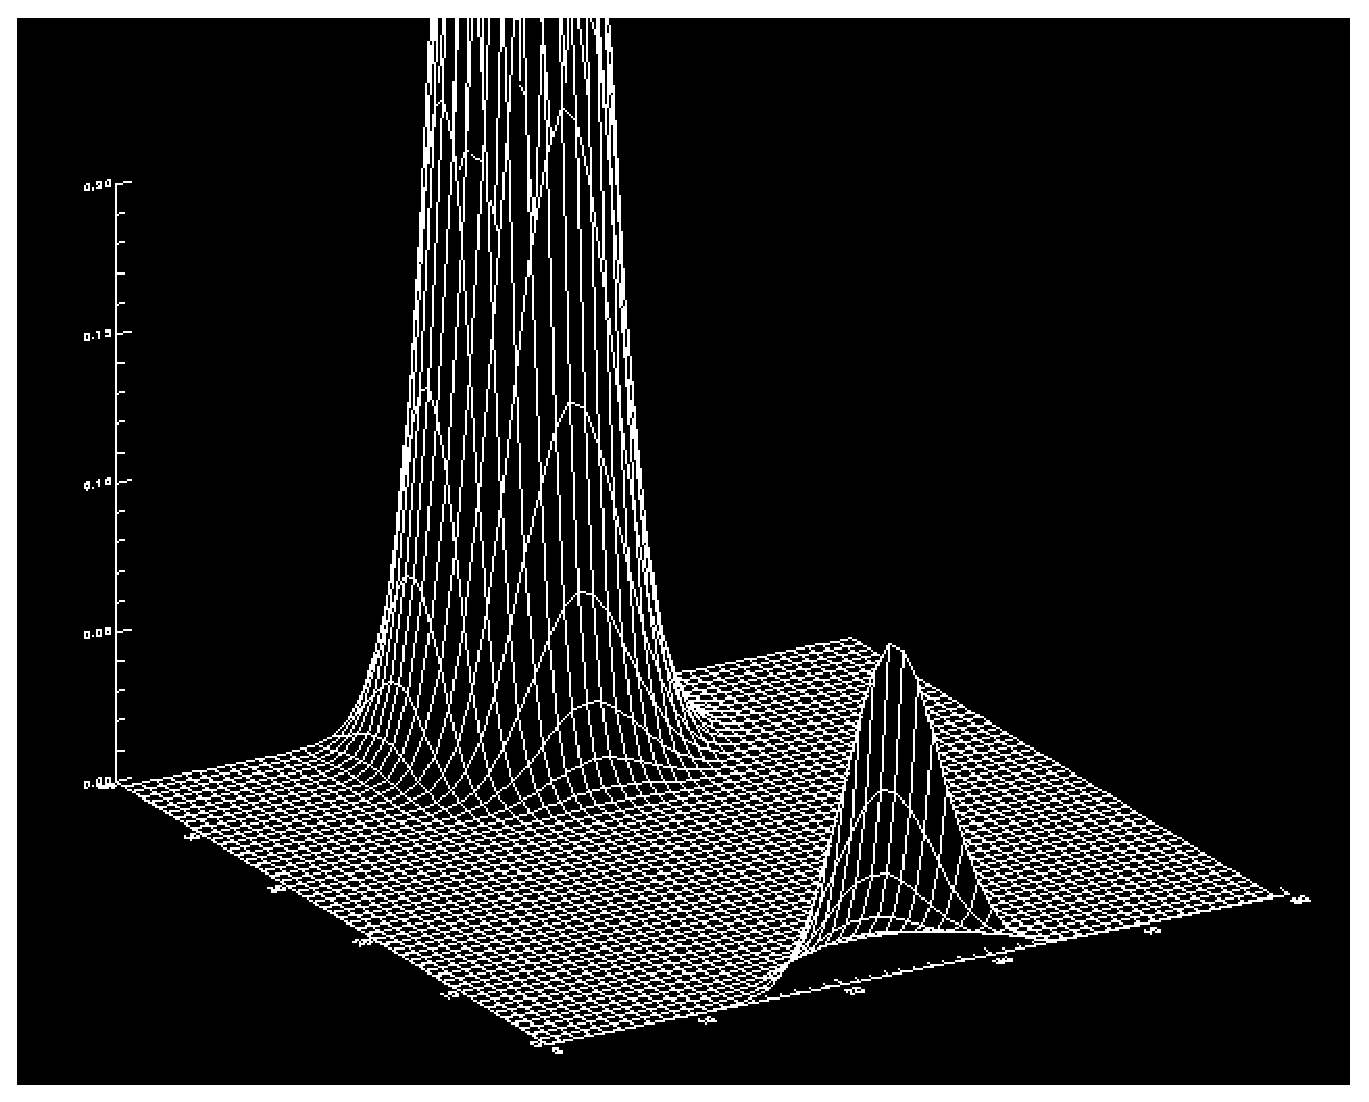
\includegraphics[width=0.49\columnwidth]{./full/test/deltas_10}
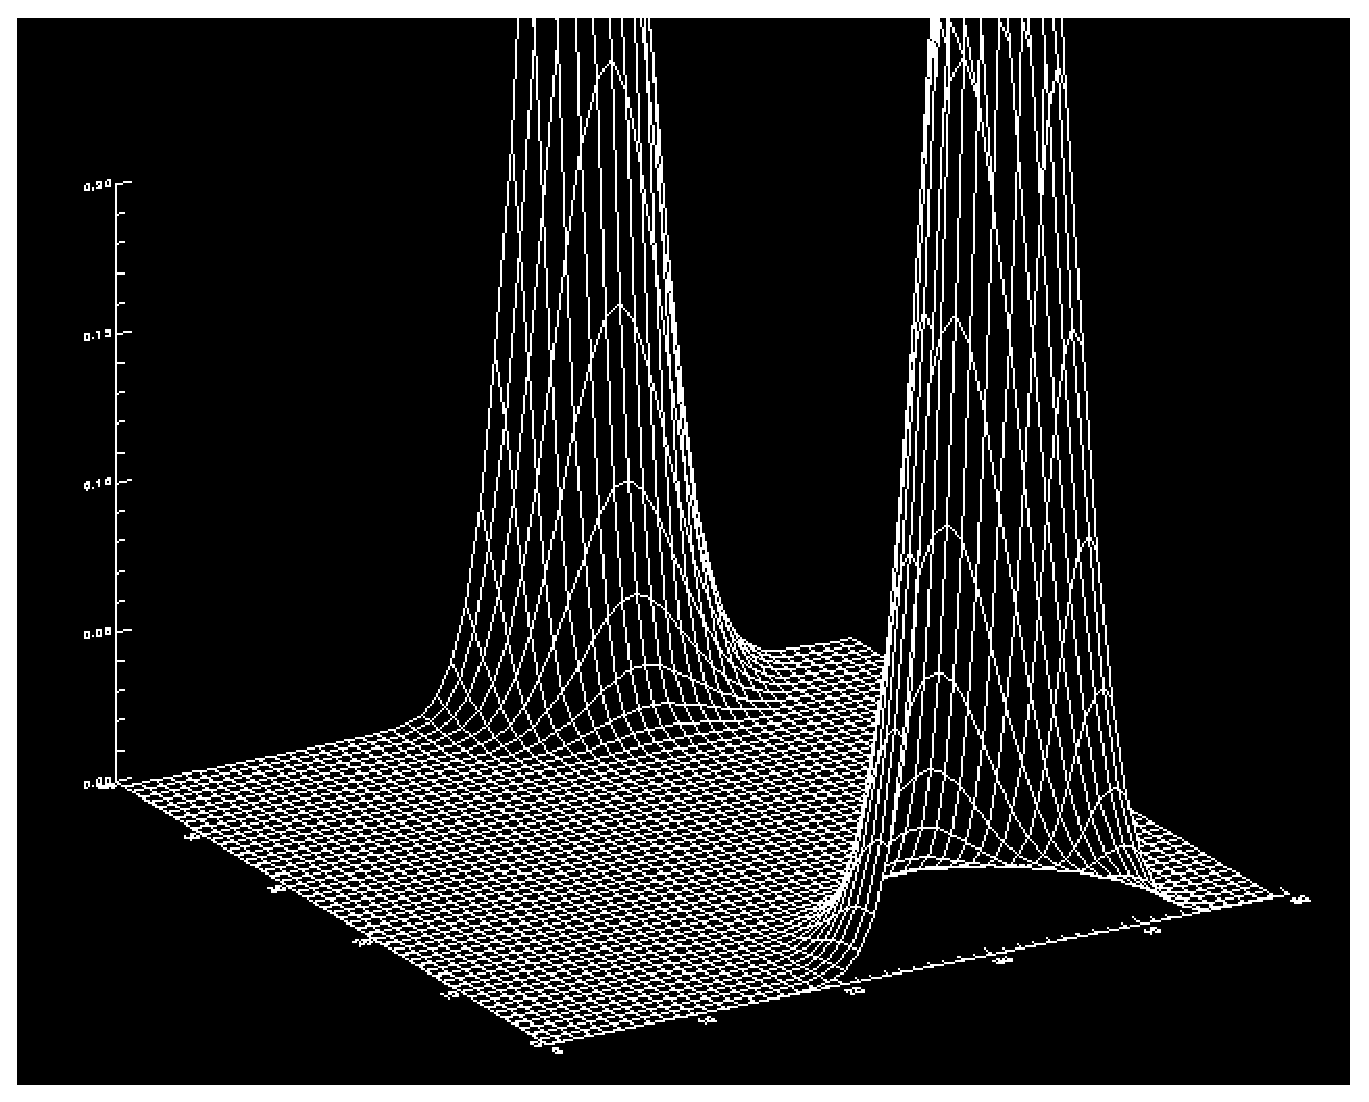
\includegraphics[width=0.49\columnwidth]{./full/test/deltas_20}
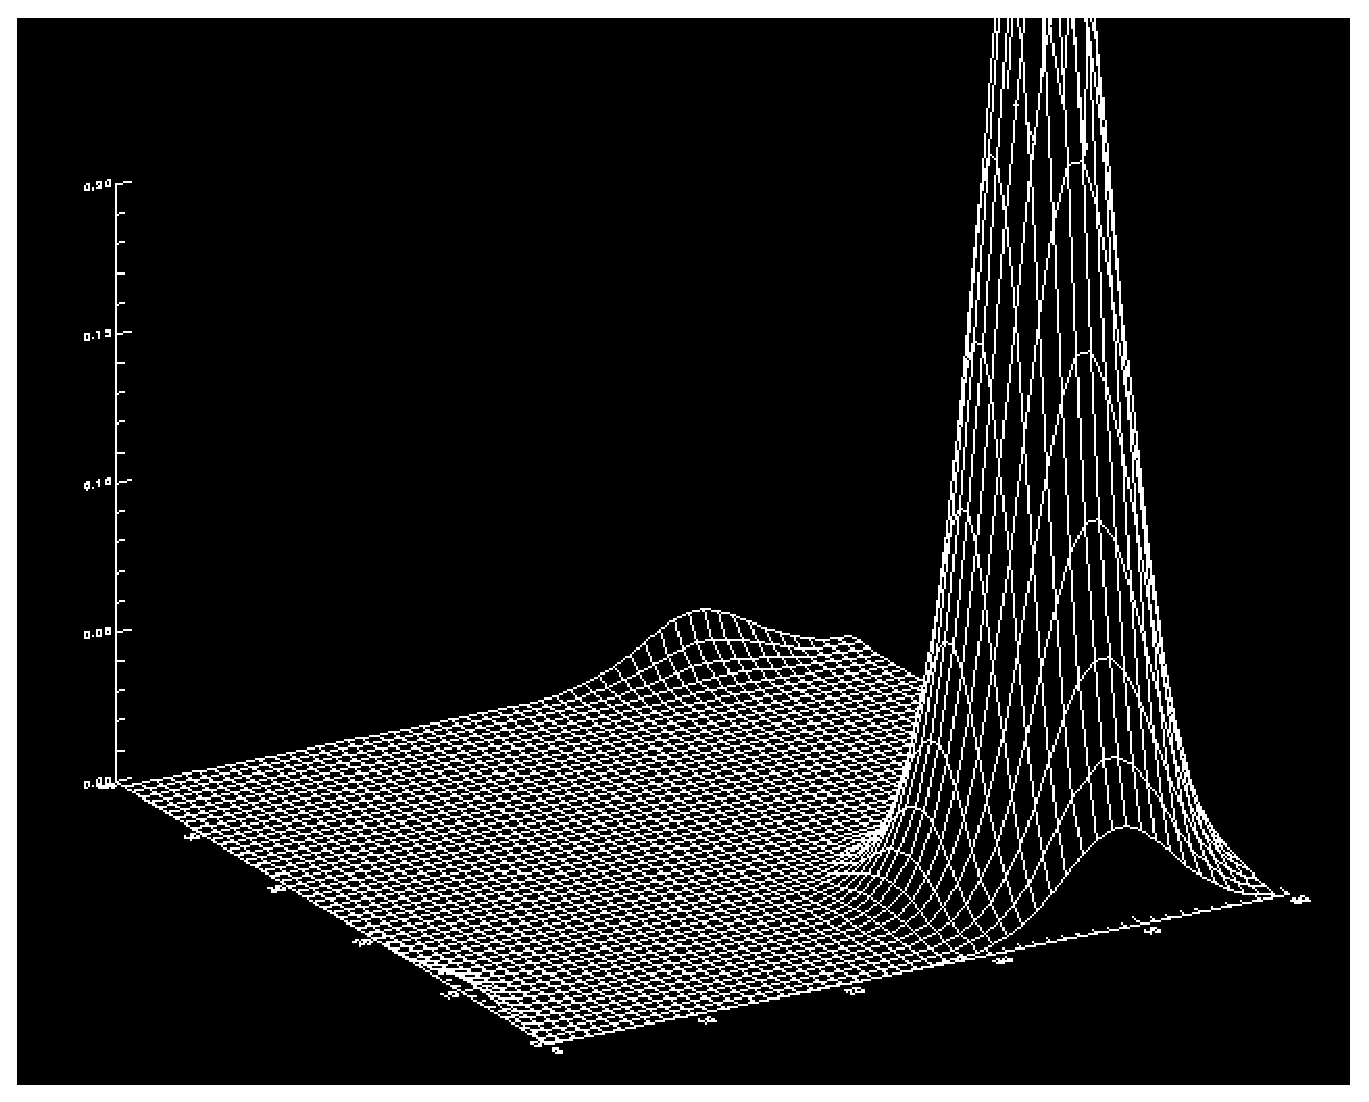
\includegraphics[width=0.49\columnwidth]{./full/test/deltas_30}
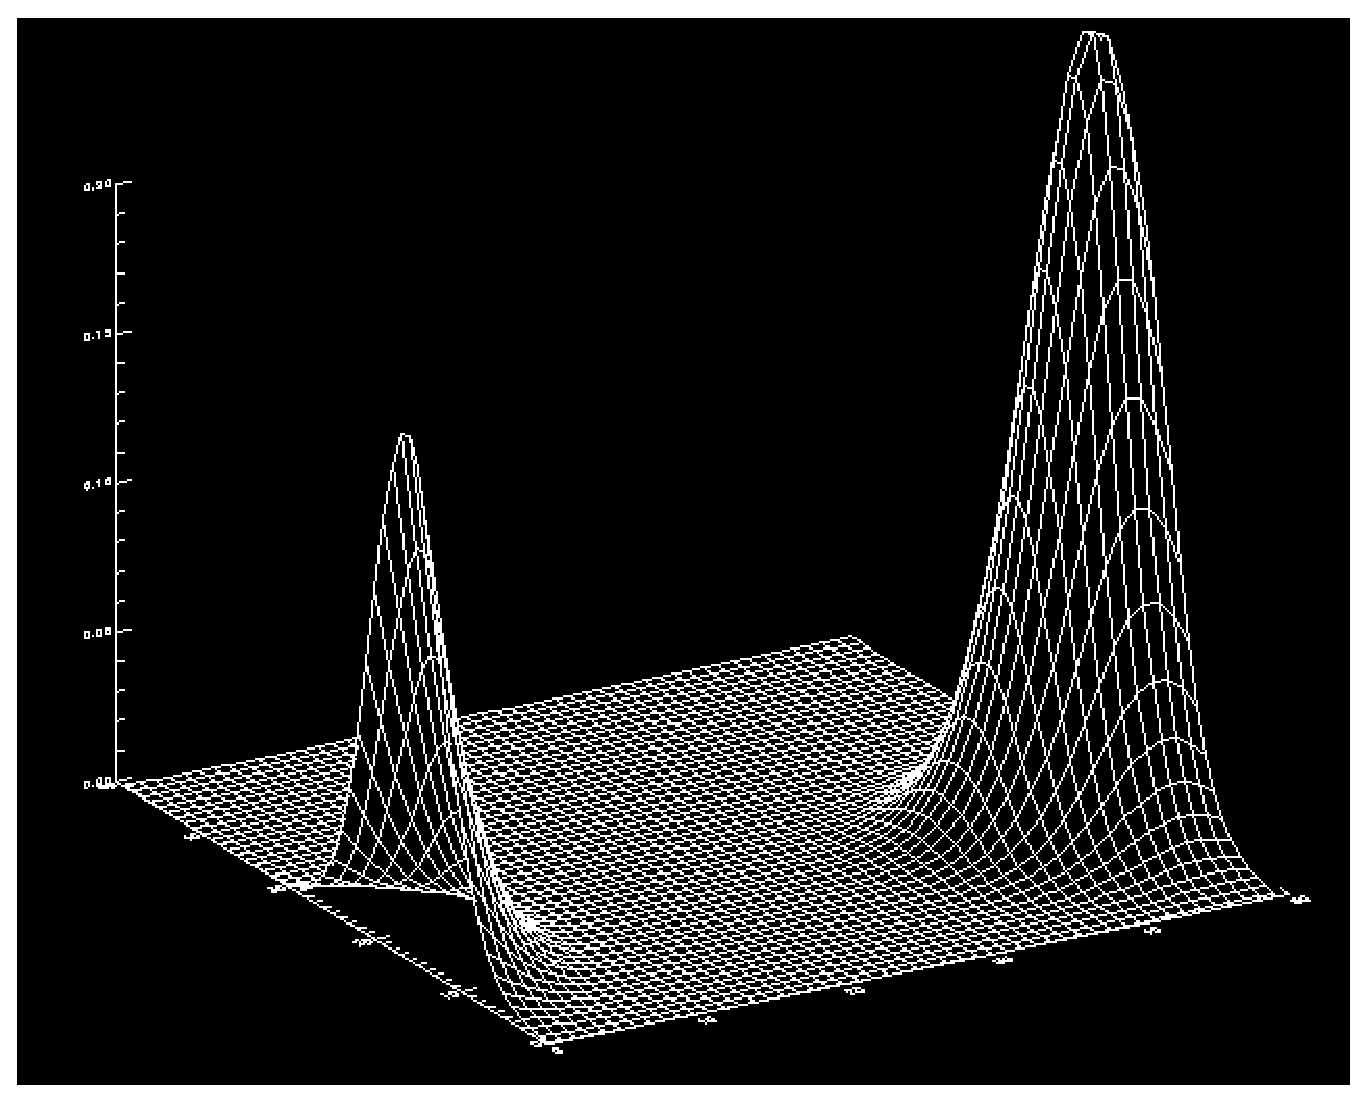
\includegraphics[width=0.49\columnwidth]{./full/test/deltas_40}
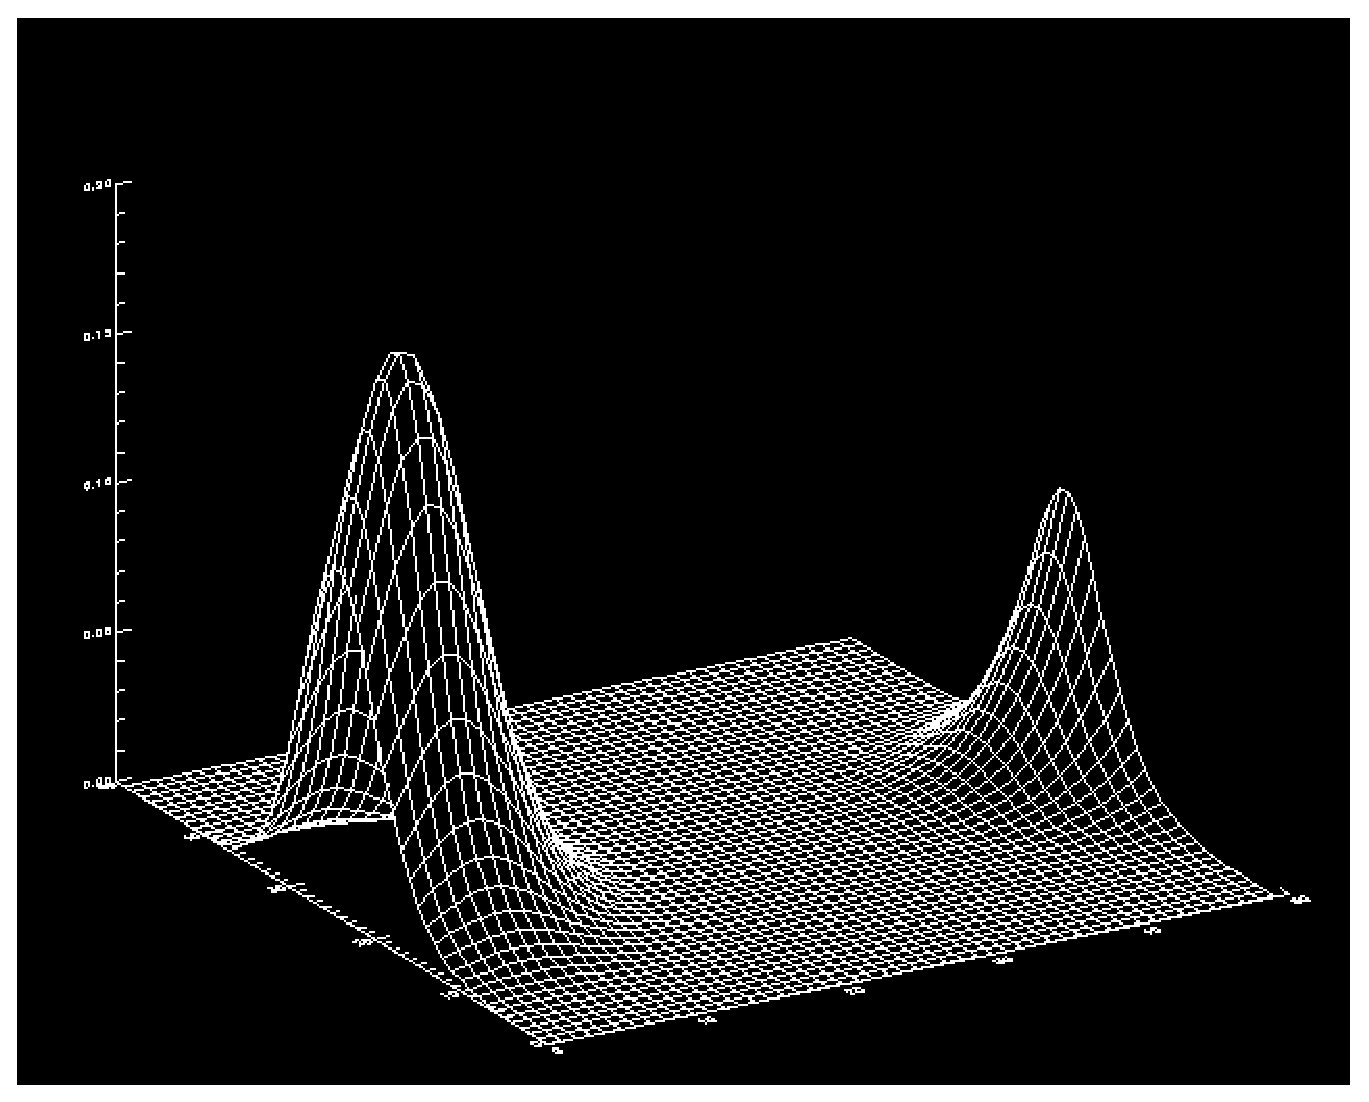
\includegraphics[width=0.49\columnwidth]{./full/test/deltas_50}
   \end{center}
\caption{The plots here show a wave-packet (or the `envelope of the wavefunction', which is the density $\psi^*\psi$) passing through all four boundaries of a 2D plane, the results were generated from a 3D code.}
\label{fig.test_bound}
\end{figure}

In testing, we explored what would happen to a wavefunction near the boundary when using a simple Goldberg algorithm -- that is, without the re-iteration of the auxiliary functions $e$ and $f$. As the edges of the system are not defined then the wavefunction appears to hit a hidden boundary. This effect was seen as a type of feedback (the wavefunction spikes up as if compressed by a potential barrier). This also resulted in a loss of mass at the boundaries whenever the wavefunction `escapes' out of the system. The feedback is obviously a numerical problem as the edge of the system should not be a barrier. With a smooth transition across the edge of the system then there should be no feedback.

An interesting result from running a wave-mechanics code is that of a stationary gaussian wave that is allowed to freely disperse without an underlying potential. If the code includes periodic boundaries then it is possible for the edges of the gaussian wavefunction to disperse across the boundary and eventually come back to interfere with itself.

The result is something that is akin to beat phenomena, where two frequencies compete with each other. The gaussian wavepacket is the envelope ($\psi \psi^*$) with a certain characteristic length but the wavefunction also has a (higher) carrier frequency. When the wave interferes with itself (or a neighbouring piece of the Universe, adopting the cosmology analogy where a simulation is quasi-infinite) under periodic boundaries the envelope acquires an additional frequency on top of the underlying gaussian envelope.

A brief look at this effect is presented in figure \ref{fig.interfere}. The results were generated using a 1D code that implements periodic boundary conditions, the outputs are at timesteps $0, 2000, 3000, 4000$. The effect of interference is minorly apparent in the second-last output but becomes a dominant feature in the last output where it is assumed that the wavefunction has passed through the boundary on both sides wrapped back in upon itself.

\begin{figure}[htb]
   \begin{center}
     %\leavevmode

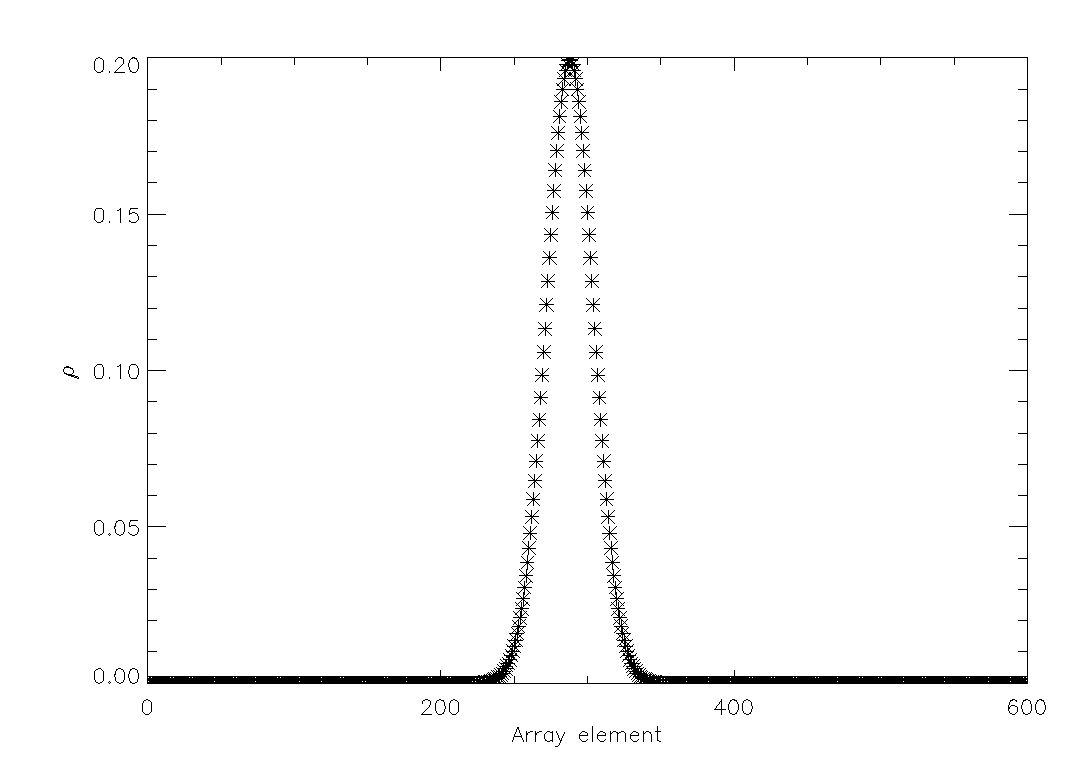
\includegraphics[width=0.49\columnwidth]{./full/periodic/rho.eps}
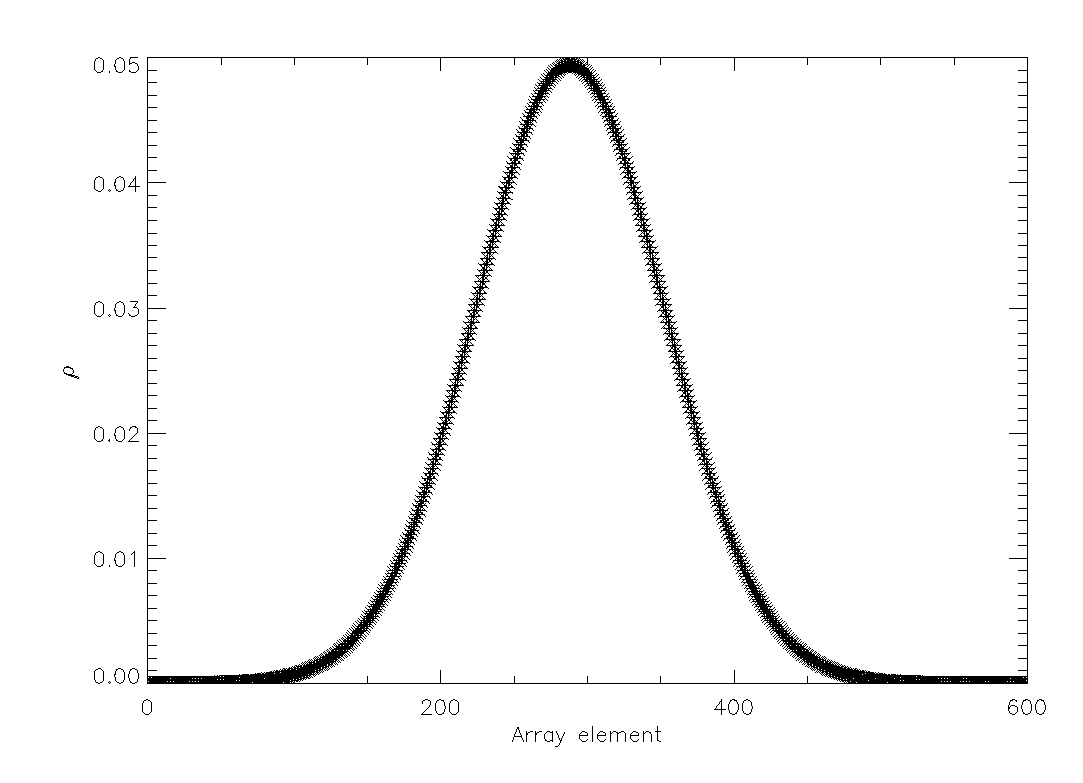
\includegraphics[width=0.49\columnwidth]{./full/periodic/rho_ev_2000.eps}
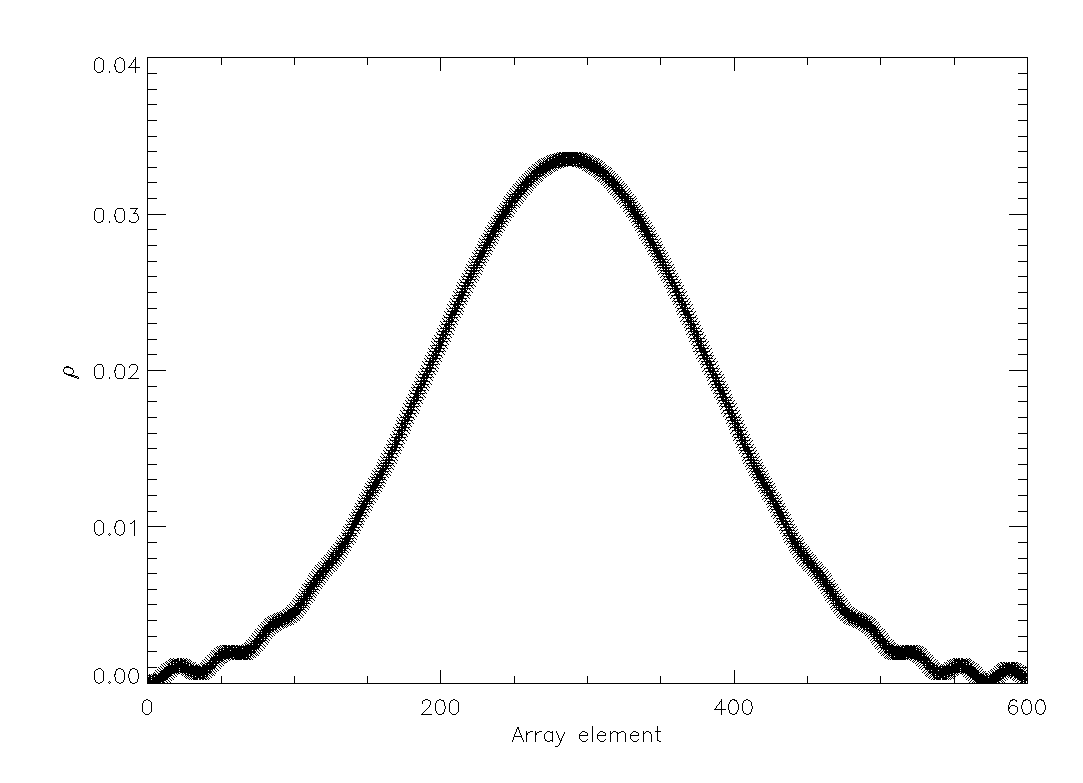
\includegraphics[width=0.49\columnwidth]{./full/periodic/rho_ev_3000.eps}
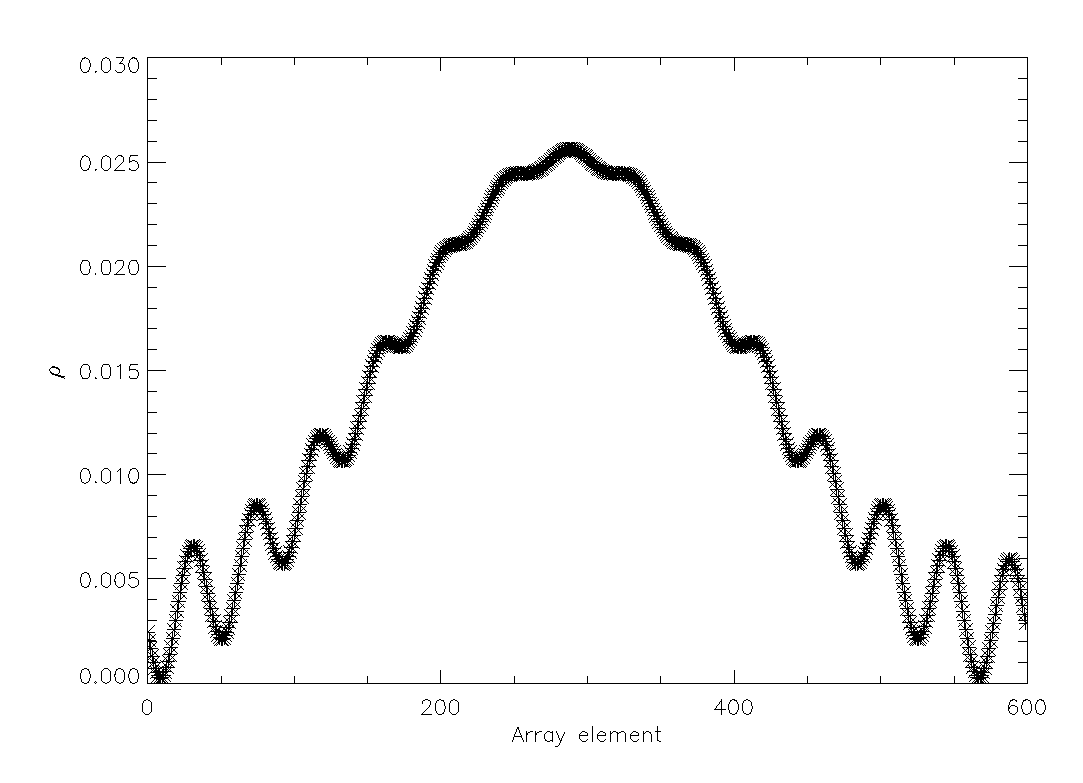
\includegraphics[width=0.49\columnwidth]{./full/periodic/rho_ev_4000.eps}

   \end{center}
\caption{The outputs at timesteps of $t = 0, 2000, 3000, 4000$. The initial gaussian wave-packet $\psi^*\psi$ is thin and centred within the box. Periodic boundaries were implemented. The wave-packet disperses and self-interferes once the wavefunction has crossed significantly pass the boundary.}
\label{fig.interfere}
\end{figure}

Such a result is important when considering the full cosmological simulations later. We need to ask ourselves what do we expect when the wavefunction crosses over the boundary and how far must it travel in order to create this (feedback) interference effect.

The results from the cosmological simulations in a later subsection (\ref{cos_sim}) have greater variation in the range of densities than first expected. In this later subsection I show a comparison with the `industry standard' code Gadget which is providing our benchmark and hence provides what we expect from a cosmological code. The variation shown in the density outputs from wave-mechanics is far greater than that of Gadget. At first we considered that this variation was due to feedback this is now thought to be unlikely. From the wave-mechanics results it is clear that the waves (in general) have not crossed the entire length of the box, it even appears unlikely that any wave has travelled half of one box length.

In our study of feedback in this section the wavefunction must have dispersed a minimum of one box length and hence it gives a self-interaction pattern (shown in figure \ref{fig.interfere}). Here the wave-packet $\psi^*\psi$ (the density) has dispersed and is free of an internal or external potential. As is clear from the figure, the central density decreases in height as the width increases.

We performed several tests of the codes in all dimensions, with one of the tests being to see how fast a wavefunction will disperse. We found that the dispersion and subsequent feedback effect is dependent on the choice of $\nu$. Large values of $\nu$ will allow for faster dispersion and hence feedback will be seen earlier. However, such an effect requires the waves to pass far across each boundary which is further than should be typically allowed in a cosmological simulation. The typical $\nu$ values used in the cosmological simulations are quite small -- for example, $10^{-7}$; during our tests such a small value showed only a small degree of dispersion and hence the time required to see feedback is far longer than the simulation time.

We modified this test to include a second gaussian peak in the box. The peaks are situated in such a way that the system is symmetric about the midpoint of the $x$-axis. We performed three such tests and kept the initial conditions the same (except for an additional kinetic boost in the second test). In the first case we had no gravity; the second test involved an initial kick in velocity but no gravity while the third test had no initial kick in velocity but the peaks were subjected to gravitational interaction.

In the first test (see figure \ref{fig.twodisp}) we wished to see what happened when the two peaks are allowed to freely disperse with no initial kinetic energy and are not subject to the force of gravity. As expected the two peaks disperse and eventually overlap each other. The pattern of the overlap is what we expect from a wave-mechanics code. We see interference effects when the wavefunctions over lap; ideally, we would not see this in a classical code which raises a point of contention when using a wave-mechanics code. Such effects should be minimized when simulating a classical system.


\begin{figure}[htb]
   \begin{center}
     %\leavevmode

\includegraphics[width=0.49\columnwidth]{./full/BB/delta.eps}

\includegraphics[width=0.49\columnwidth]{./full/BB/delta_ev60.eps}

\includegraphics[width=0.49\columnwidth]{./full/BB/delta_ev100.eps}

\includegraphics[width=0.49\columnwidth]{./full/BB/delta_ev120.eps}

\includegraphics[width=0.49\columnwidth]{./full/BB/delta_ev140.eps}

\includegraphics[width=0.49\columnwidth]{./full/BB/delta_ev180.eps}

   \end{center}
\caption{This figure shows the dispersion of gaussian peaks in a box.  The output times are at timesteps of $0, 60, 100, 120, 140, 180$.}
\label{fig.twodisp}
\end{figure}

Another test of our code is to provide two gaussian peaks with some initial kinetic energy, rather than let them freely disperse. We also omitted gravity from this test. The results are shown in figure \ref{fig.twokin}; we plot normalized density, $\rho$, against a normalized length, $x$. This simulation used 512 grid elements. The two peaks have met by timestep 40 and are almost apart in the last plot at timestep 100. The speed of dispersion is set by the parameter $\nu = \hbar/m$.

\begin{figure}[htb]
   \begin{center}
     %\leavevmode

\includegraphics[width=0.49\columnwidth]{./full/CC/delta.eps}

\includegraphics[width=0.49\columnwidth]{./full/CC/delta_ev20.eps}

\includegraphics[width=0.49\columnwidth]{./full/CC/delta_ev40.eps}

\includegraphics[width=0.49\columnwidth]{./full/CC/delta_ev60.eps}

\includegraphics[width=0.49\columnwidth]{./full/CC/delta_ev80.eps}

\includegraphics[width=0.49\columnwidth]{./full/CC/delta_ev100.eps}

   \end{center}
\caption{In this figure two gaussian peaks with some initial kinetic energy pass through each other and their evolution is observed. The peaks move with a constant velocity. The outputs are at timesteps of $0, 20, 40, 60, 80, 100$.}
\label{fig.twokin}
\end{figure}

One of the most important tests in one dimension is that of two peaks passing through each other under the influence of gravity. In this test the peaks had no initial kinetic energy. The results of this test are shown in figure \ref{fig.twograv}. The peaks appear to move slowly at first then accelerate through each other; the initial timesteps show little happening as the attraction towards each other is slow. The maximum peak achieved is when the two peaks fully meet in the middle (shown at timestep 160) but soon appear as two separate peaks not long after (timestep 200).

One of the most interesting features of this third test is that gravity appears to suppress the interference effects observed in the previous two tests. It does not, however, appear to be completely free of interference effects. This is expected as the two peaks are actually part of the same wavefunction, that is to say that they are coherent. This also explains why interference effects are seen in the previous tests. Such interference patterns, as mentioned, as not classical in nature hence should not be present in the simulation of a classical system.

\begin{figure}[htb]
   \begin{center}
     %\leavevmode

\includegraphics[width=0.49\columnwidth]{./full/AA/delta.eps}
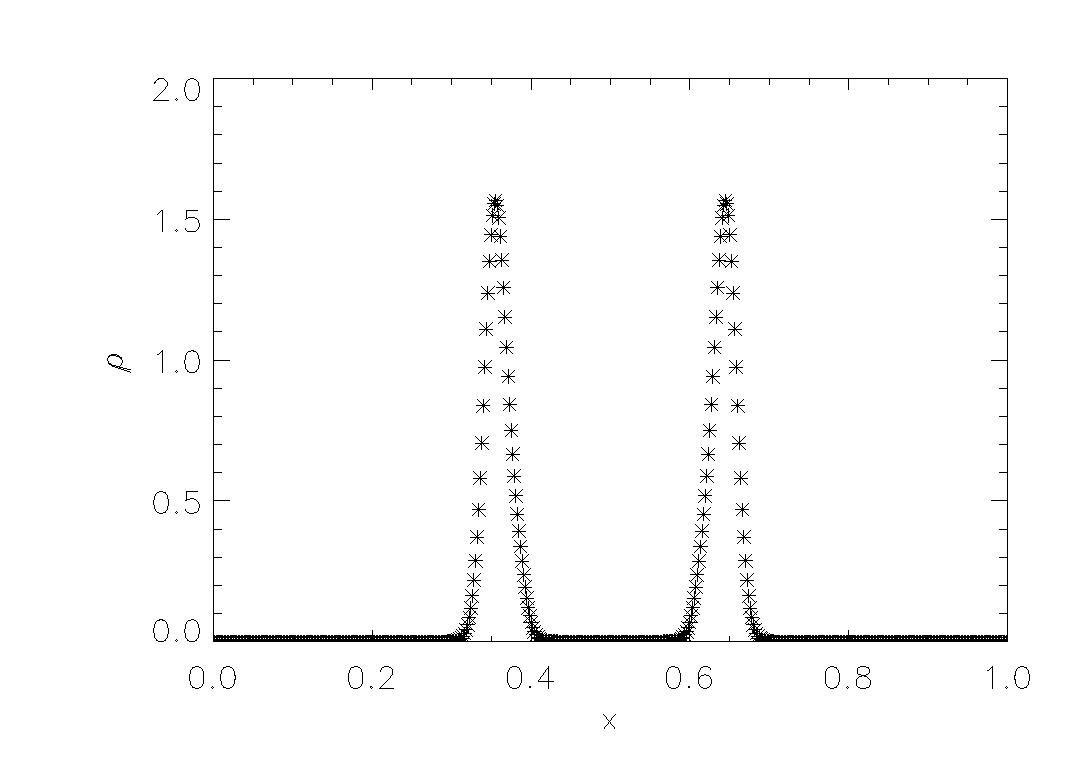
\includegraphics[width=0.49\columnwidth]{./full/AA/delta_ev40.eps}
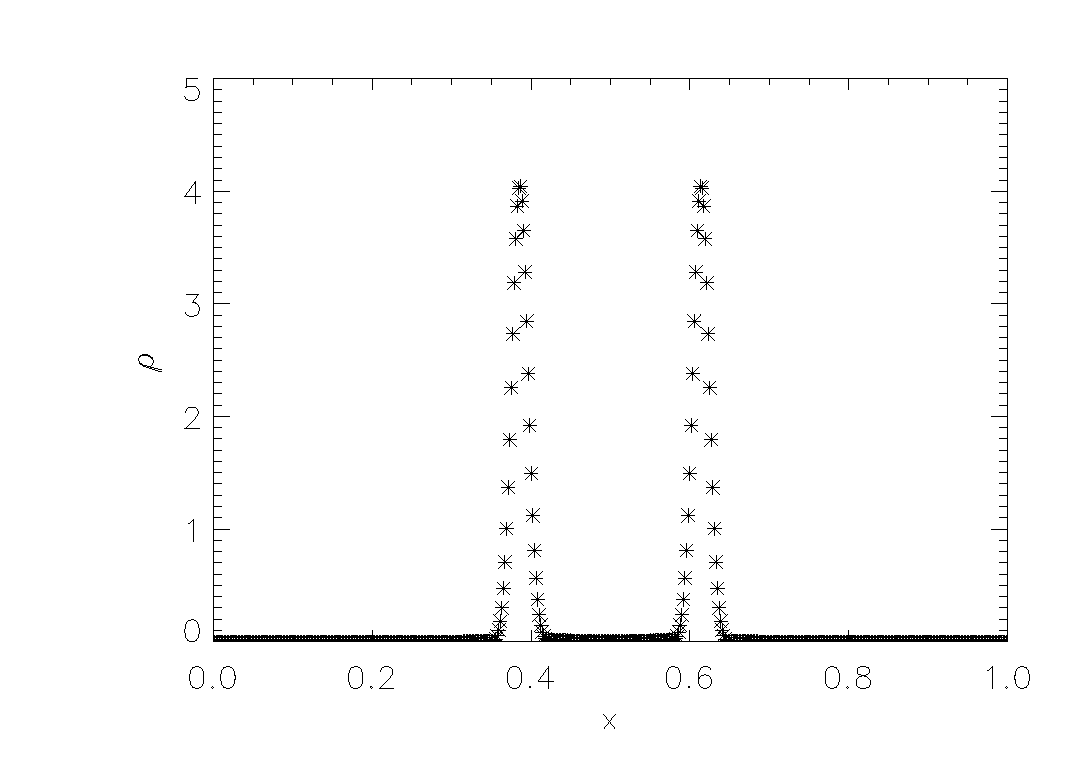
\includegraphics[width=0.49\columnwidth]{./full/AA/delta_ev80.eps}
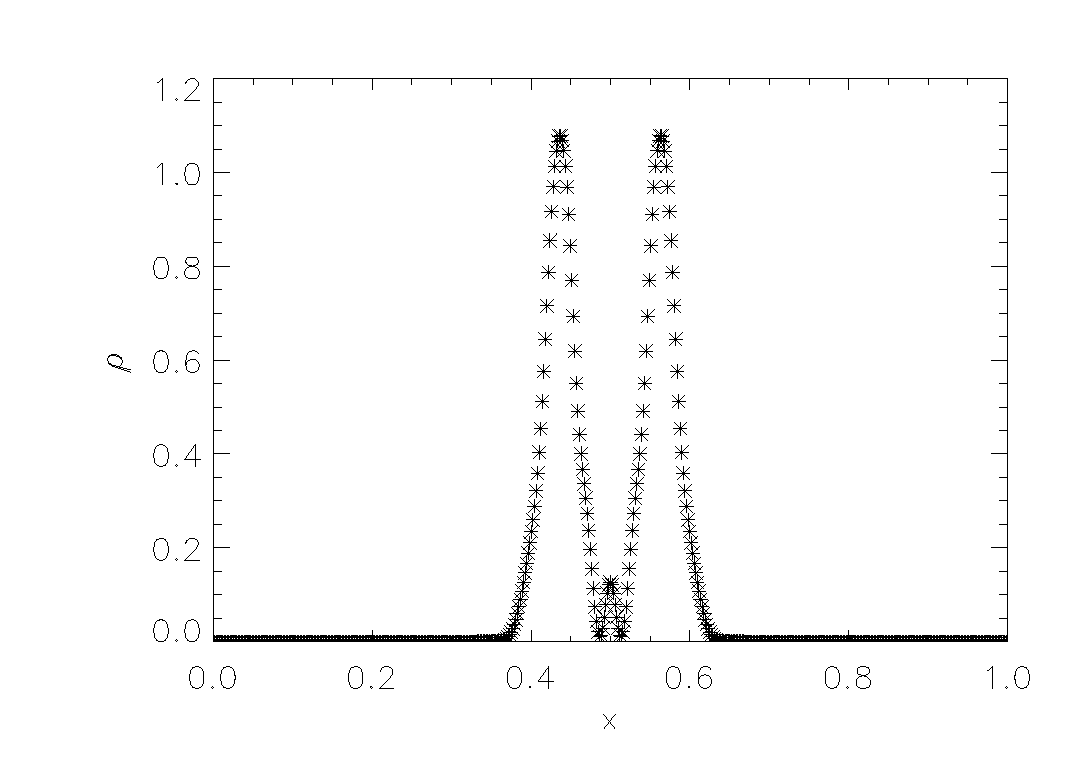
\includegraphics[width=0.49\columnwidth]{./full/AA/delta_ev120.eps}
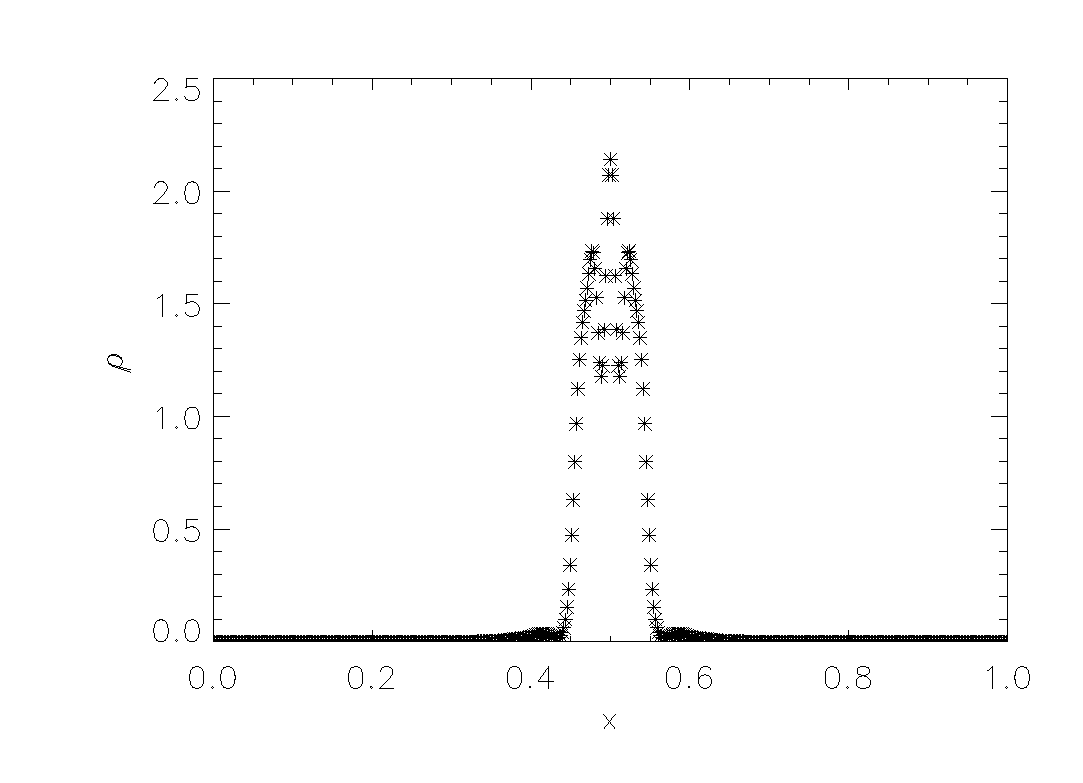
\includegraphics[width=0.49\columnwidth]{./full/AA/delta_ev160.eps}
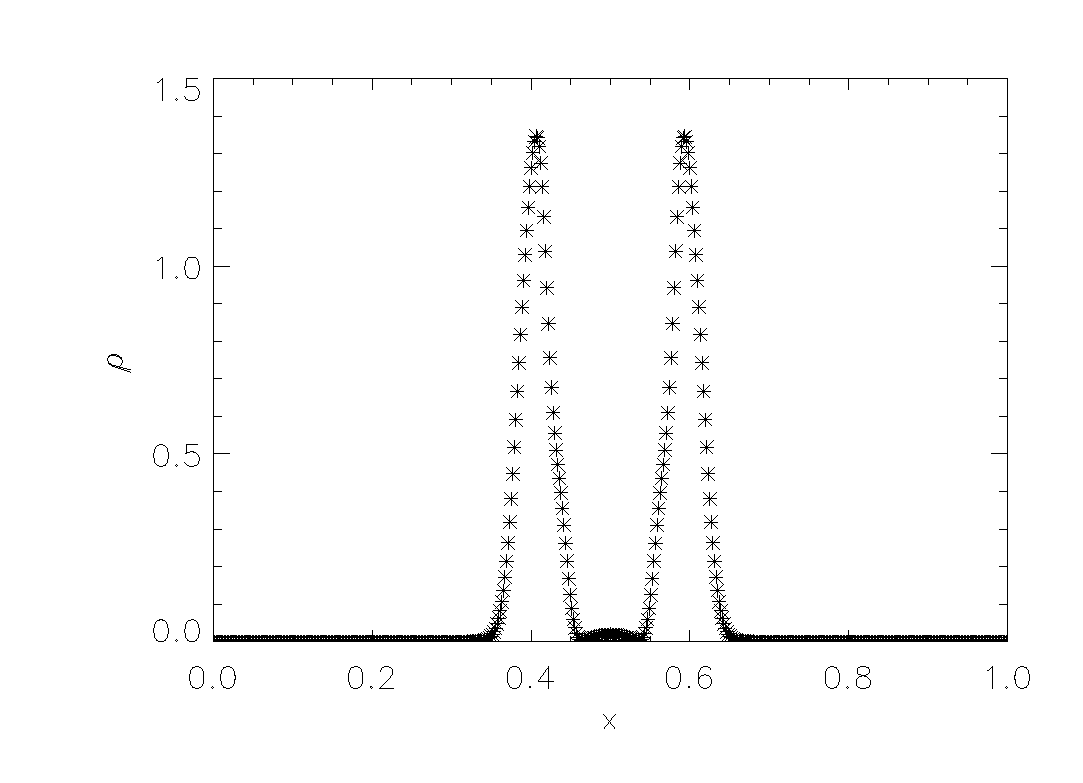
\includegraphics[width=0.49\columnwidth]{./full/AA/delta_ev200.eps}

   \end{center}
\caption{This figure shows the evolution of two gaussian peaks under the influence of gravity. The peaks move slowly at first as they attracted towards each other. The peaks speed up as they meet in the middle of the box and eventually pass through each other. The output times are at timesteps of $0, 40, 80, 120, 160, 200$.}
\label{fig.twograv}
\end{figure}


\subsection{2D Two-body gravitational interaction}
\label{twobody}
The first test of gravity in the 3D wave-mechanics code was that of a two-body gravitational interaction. In a traditional $N$-body code this test would involve two point particles interacting under the force of gravity (note: it is possible to give these particles an effect length via the softening length as mentioned in Chapter \ref{ch_2}). In wave-mechanics the particles are replaced by two gaussian wave-packets. As these two wave-packets are no longer point-like then there is no concern about two-body relaxation -- a problem that was highlighted earlier in section \ref{sec.dir_nb}.

The outputs of this test are shown in the series of plots \ref{fig.twobody}, \ref{fig.twobody2}, \ref{fig.twobody3}. The full test shows the two gaussians being attracted towards one another (during timesteps, t = [0, 30]). As the two peaks move towards each other they are observed to squeeze themselves under gravity: the peaks to become taller and thinner (as seen in the plot for time 10). Interestingly, they appear to relax and then repeat the process as they move towards the system's centre of mass where the two peaks pass through one another.

The next series of plots (\ref{fig.twobody2}) shows the two peaks passing through each other. At the mid-point when the peaks overlap they display a spiky pattern akin to the interference pattern of the double slit experiment (during timesteps, t = [35, 50]). After the pass through the two peaks move apart and journey to the starting point of the opposite peak. In the plot for timestep 65 we can see that some of the mass has been left in the middle after the interaction, this eventually disappears before the next collapse but it indicates that the masses have already passed through each other. This could be a potential way of tracing astrophysical objects that resemble this simple toy model (perhaps the Bullet Cluster -- where two distinct distributions of mass have passed through one another). A residual mass should follow the interaction but eventually this mass could be attracted towards their parent peaks.

By timestep 100 we can see that the two peaks have hit their turn-around radius. The residual mass has disappeared however the two peaks sit at these positions and re-arrange themselves under internal gravitational and presumably tidal forces. Then they begin their collapse again and are attracted towards each other. This time appears to be slightly different that the first pass through, as seen in the plot of timestep 125, there is a build up of mass at the centre before the two main peaks have interacted. By timestep 140 we can see the two peaks are starting to overlap and then have passed through each other by timestep 150.

\begin{figure}[htb]
   \begin{center}
     %\leavevmode
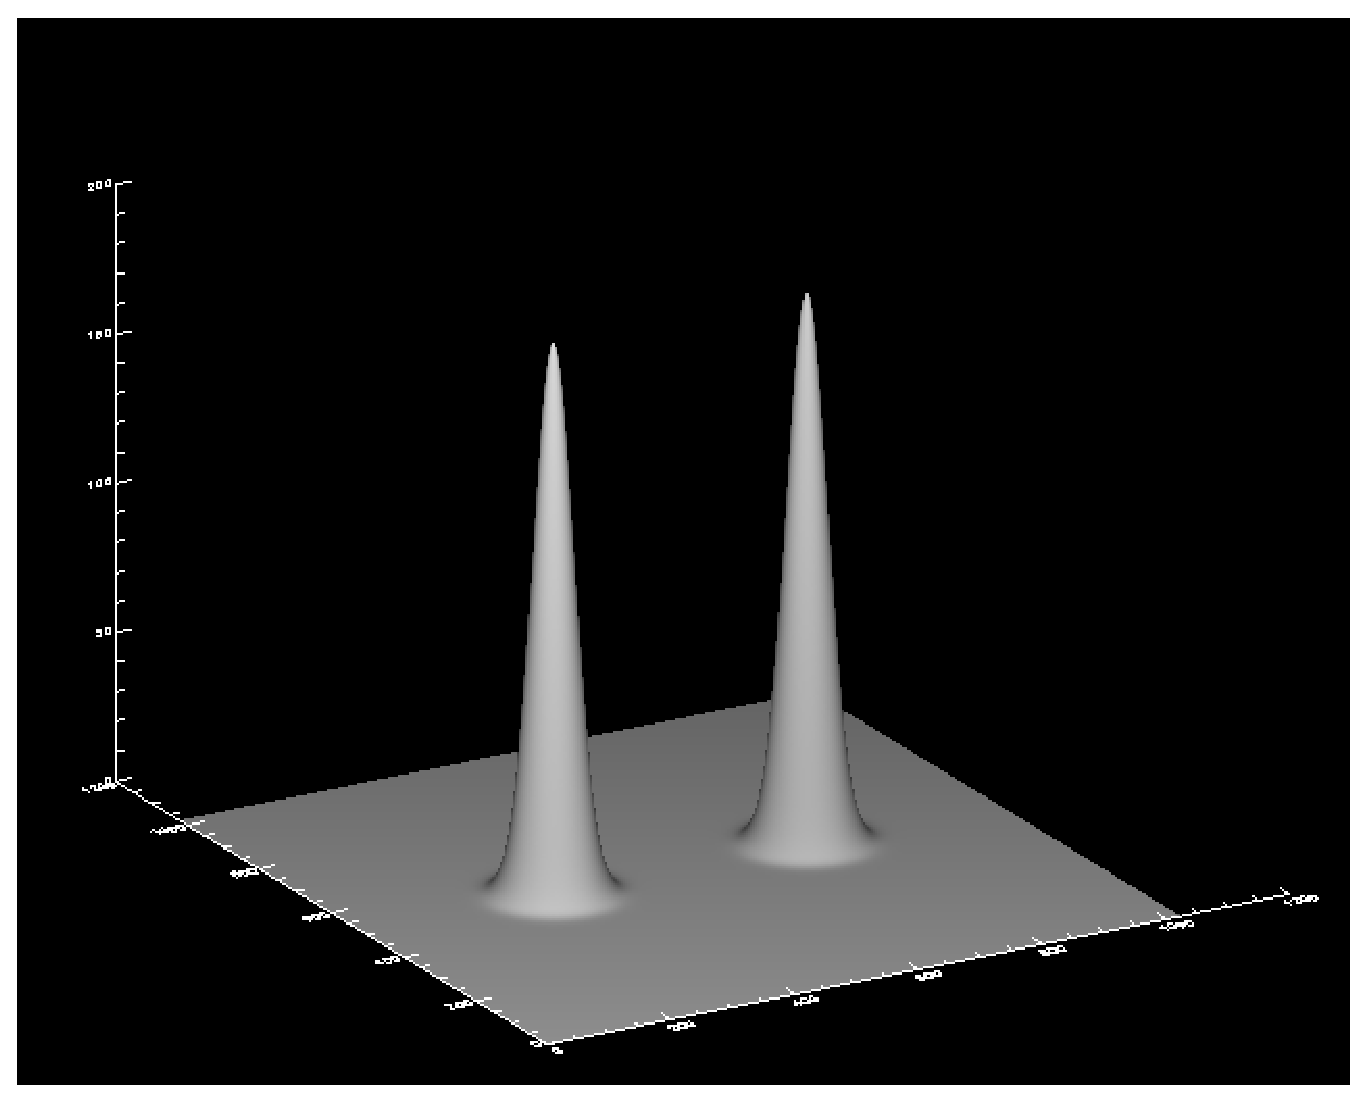
\includegraphics[width=0.49\columnwidth]{./full/twobody/deltas_000}
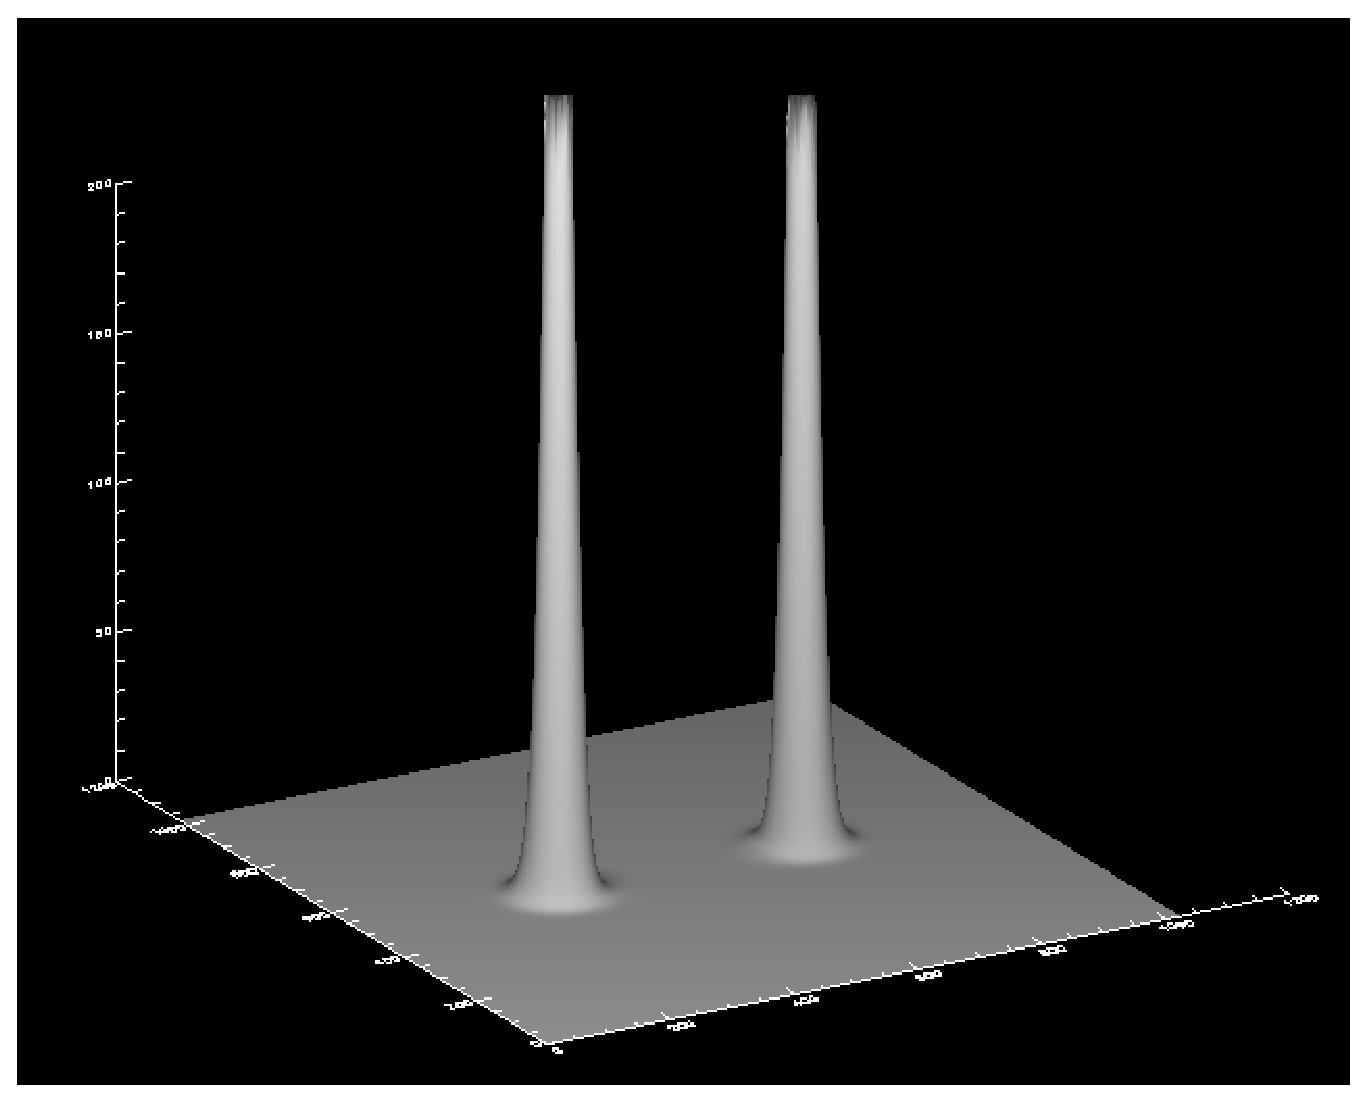
\includegraphics[width=0.49\columnwidth]{./full/twobody/deltas_010}
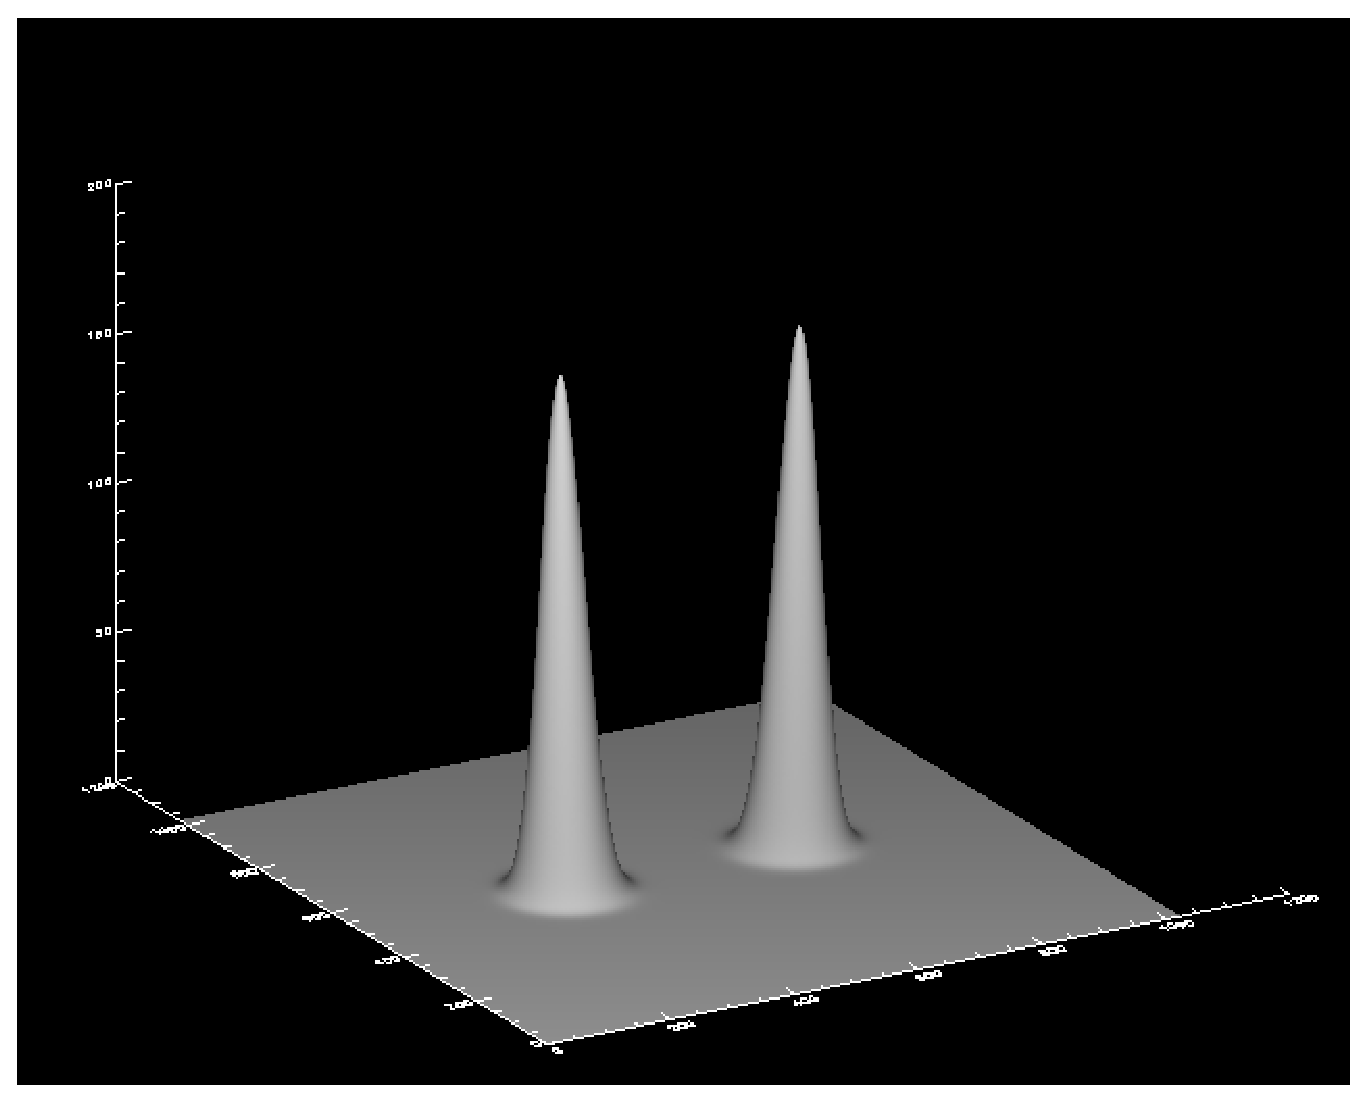
\includegraphics[width=0.49\columnwidth]{./full/twobody/deltas_015}
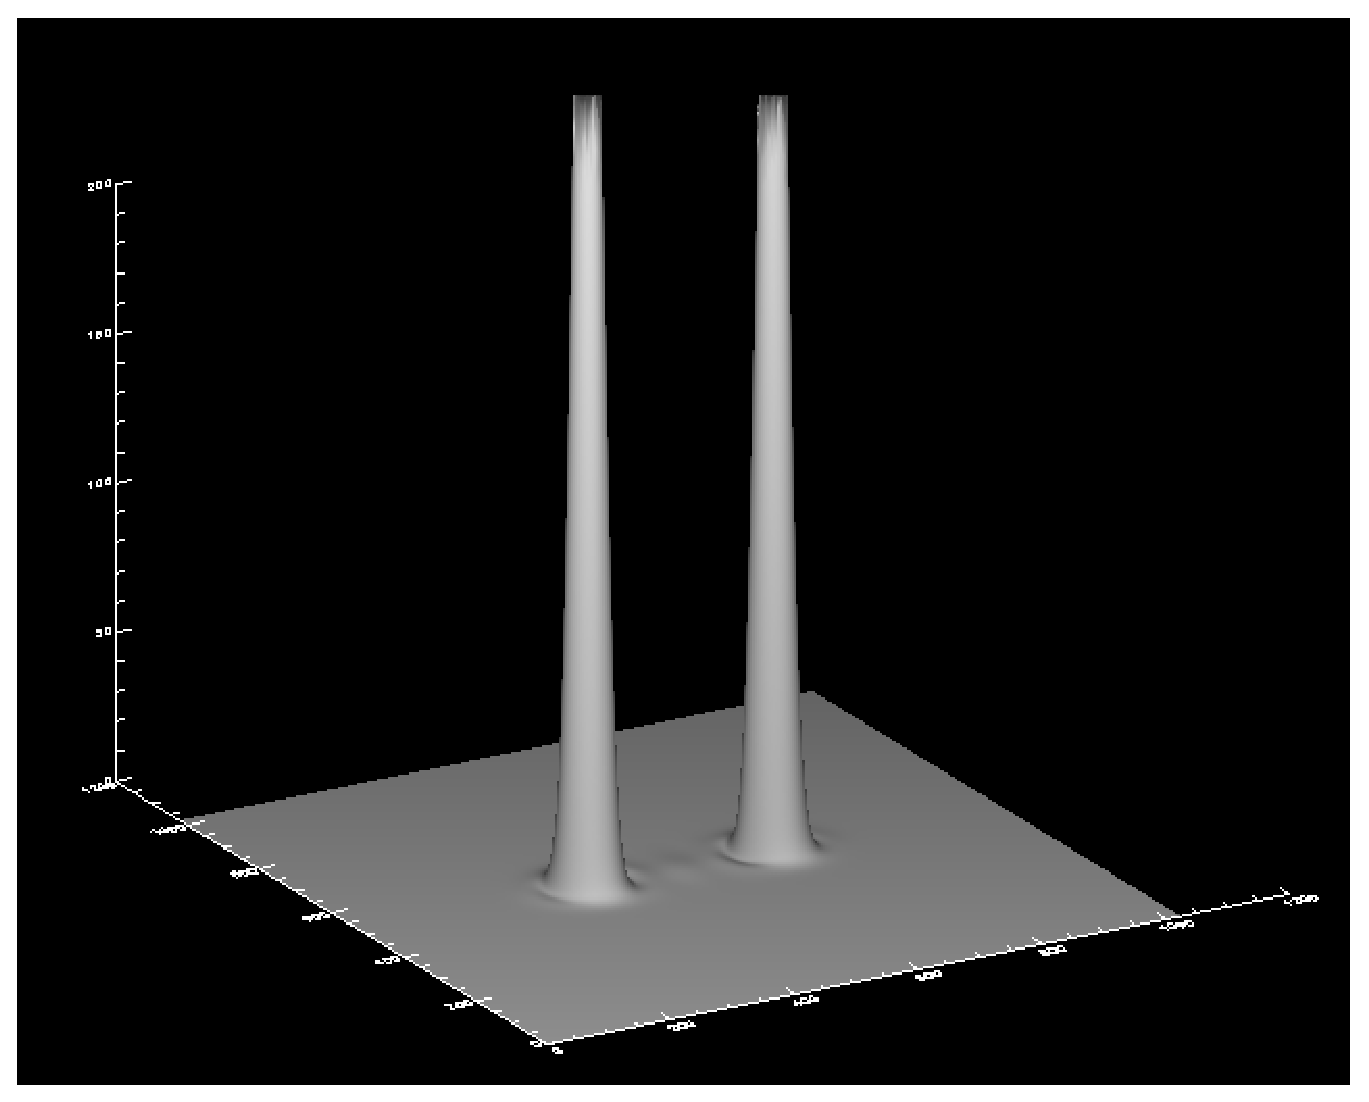
\includegraphics[width=0.49\columnwidth]{./full/twobody/deltas_025}
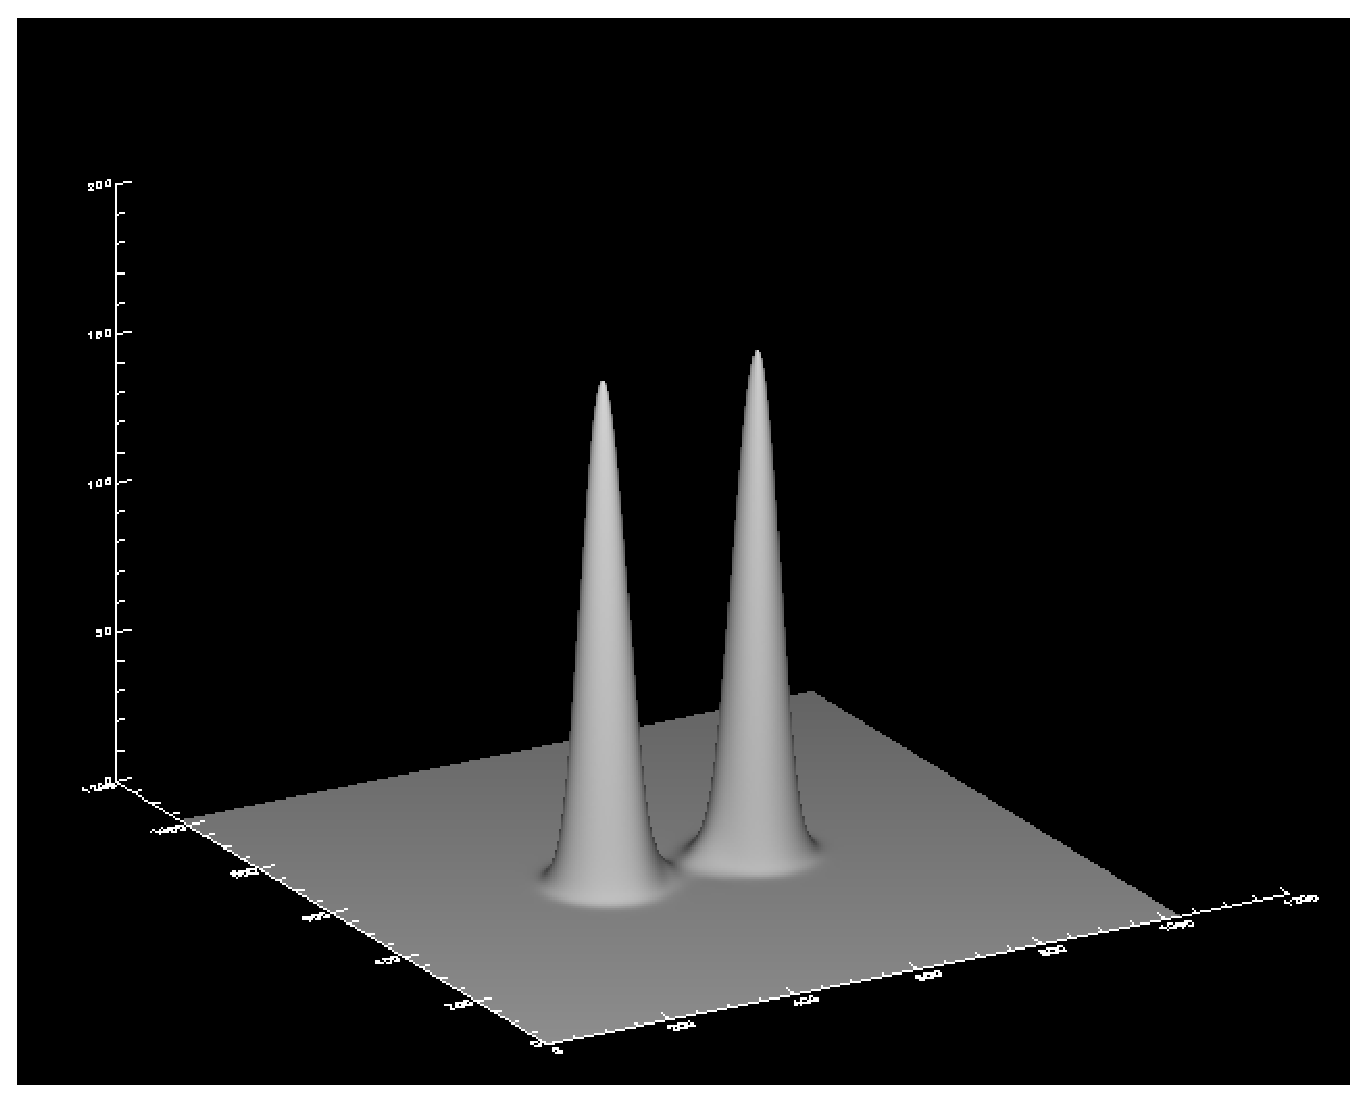
\includegraphics[width=0.49\columnwidth]{./full/twobody/deltas_030}
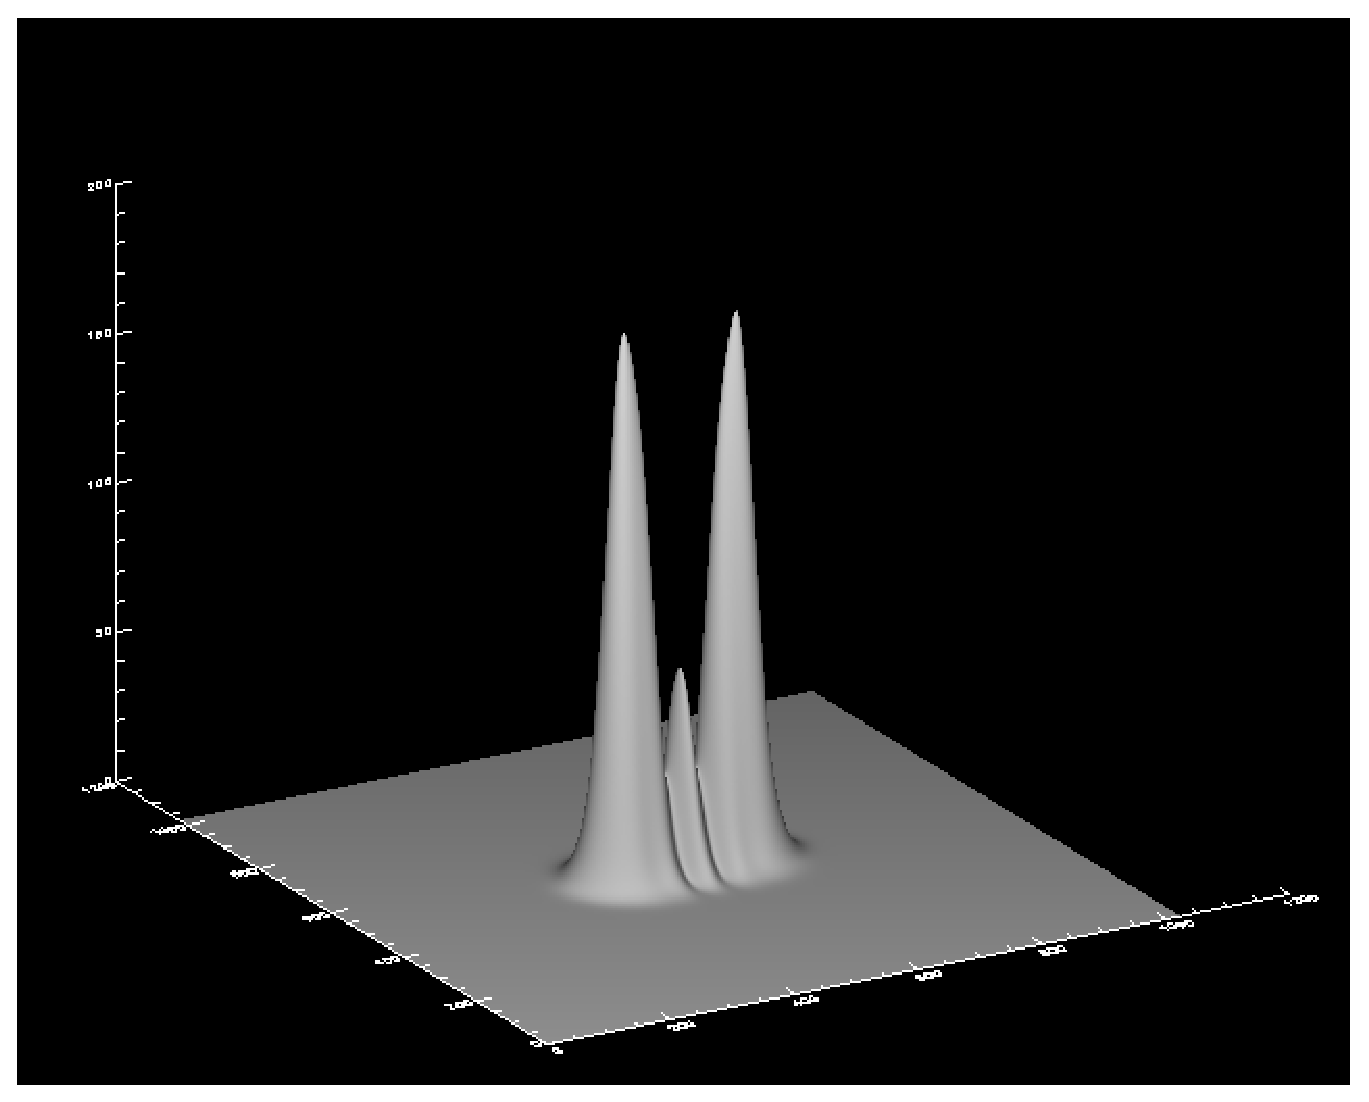
\includegraphics[width=0.49\columnwidth]{./full/twobody/deltas_035}

   \end{center}
\caption{The plots here show two gaussian wave-packets ($\psi^* \psi$, which is density) interacting under gravity. The output times are $0, 10, 15, 25, 30, 35$, they show the start of the simulation where the two peaks are attracted towards each other.}
\label{fig.twobody}
\end{figure}

\begin{figure}[htb]
   \begin{center}
     %\leavevmode
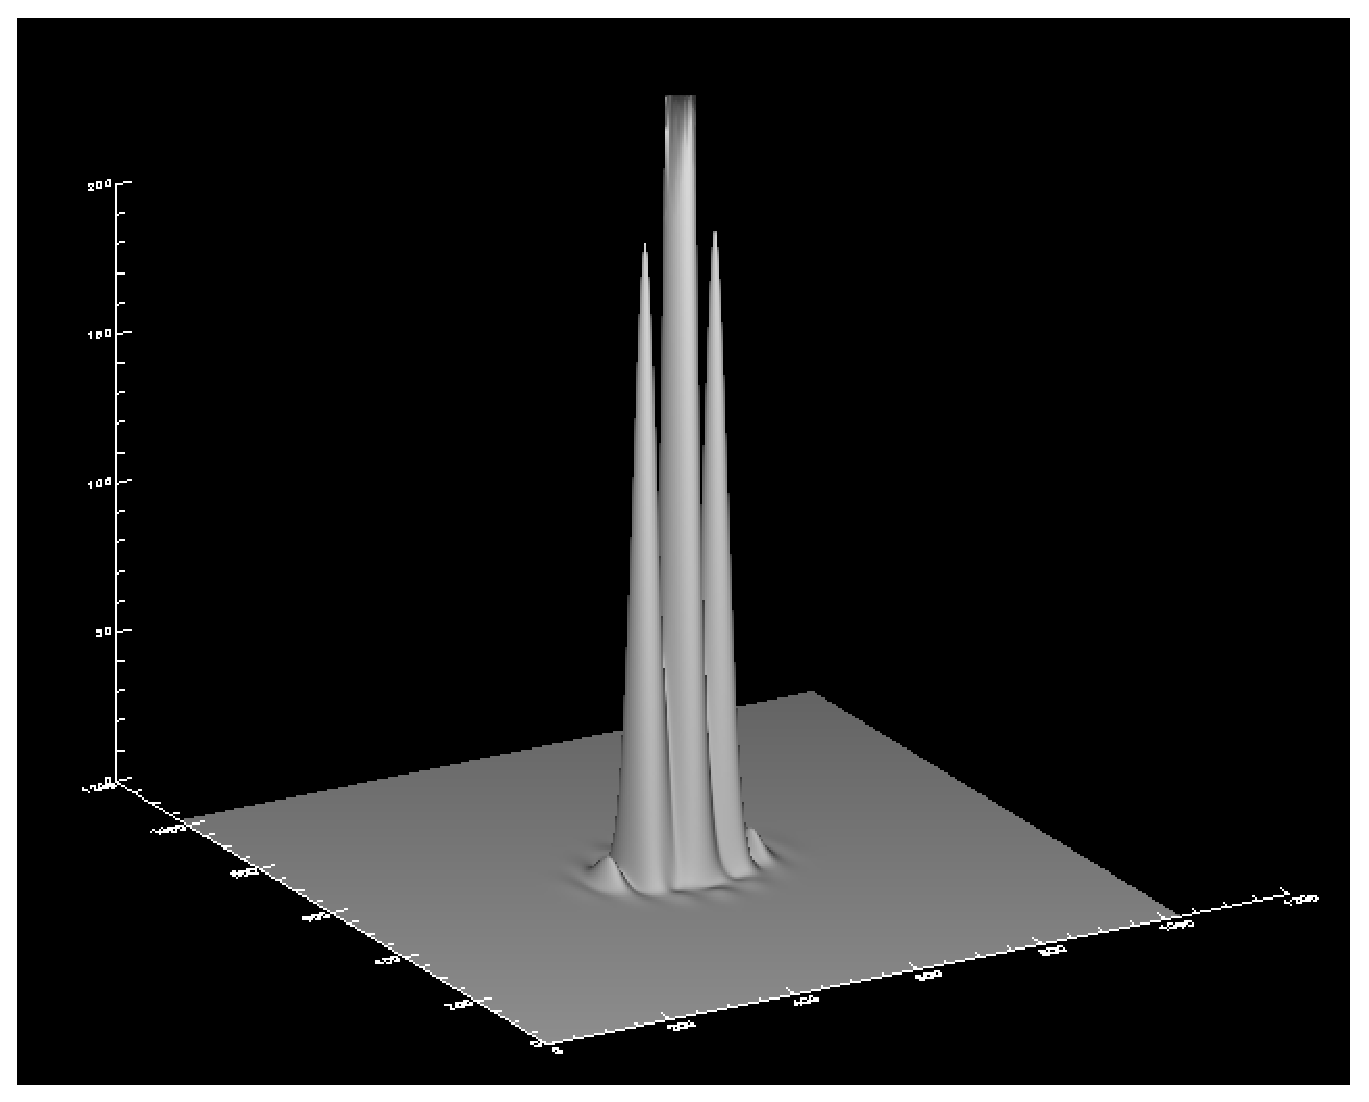
\includegraphics[width=0.49\columnwidth]{./full/twobody/deltas_040}
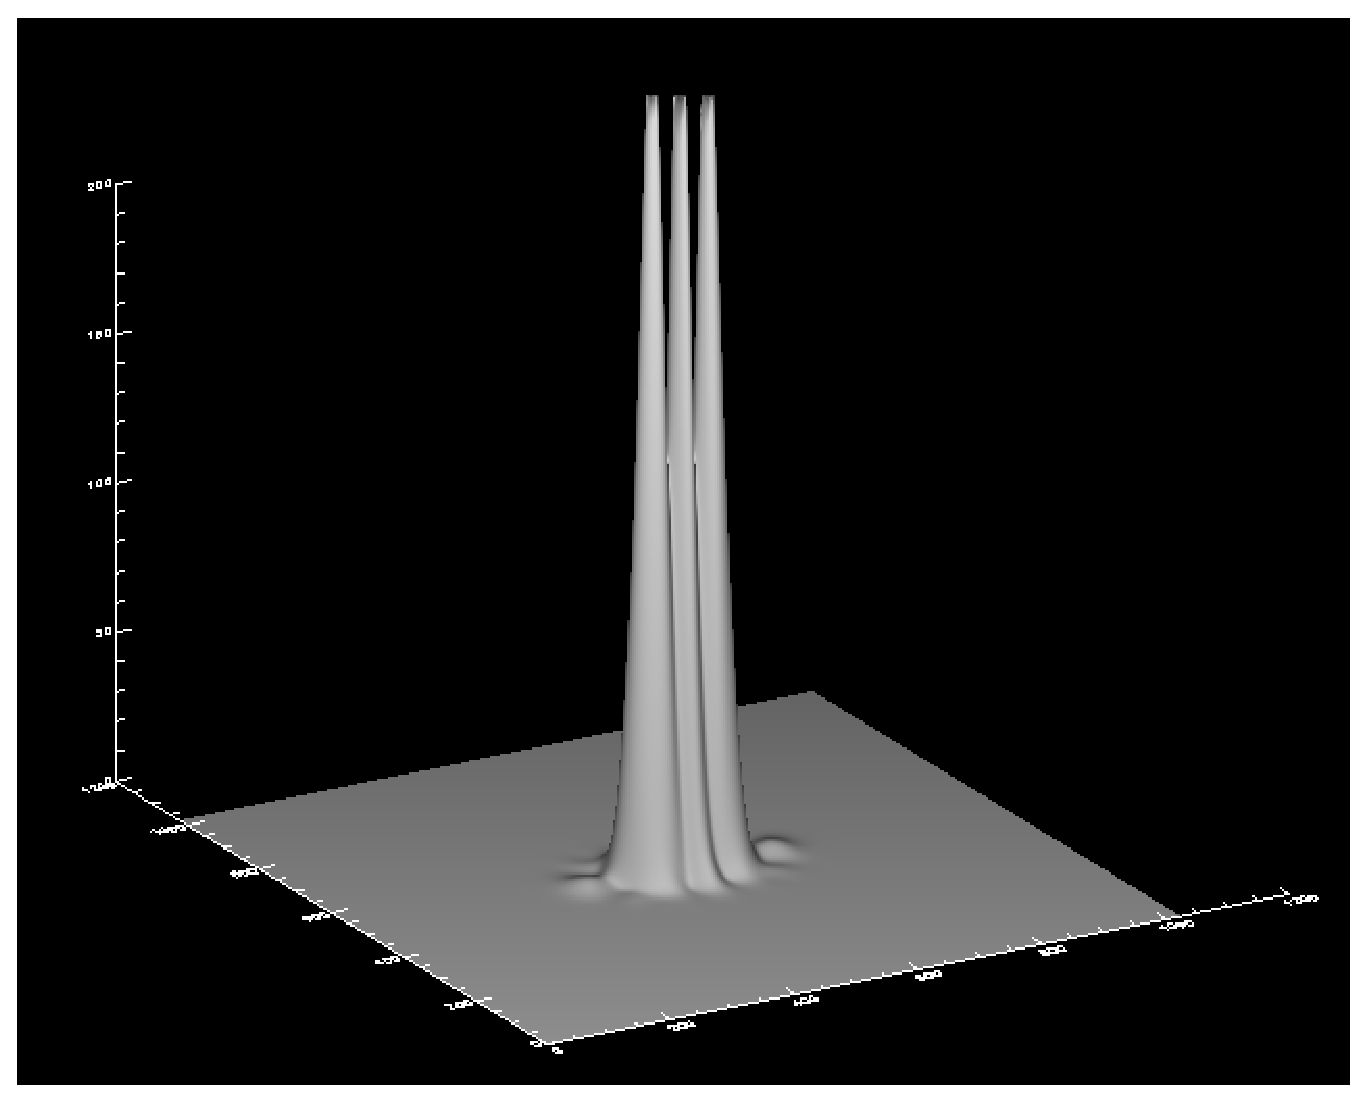
\includegraphics[width=0.49\columnwidth]{./full/twobody/deltas_045}
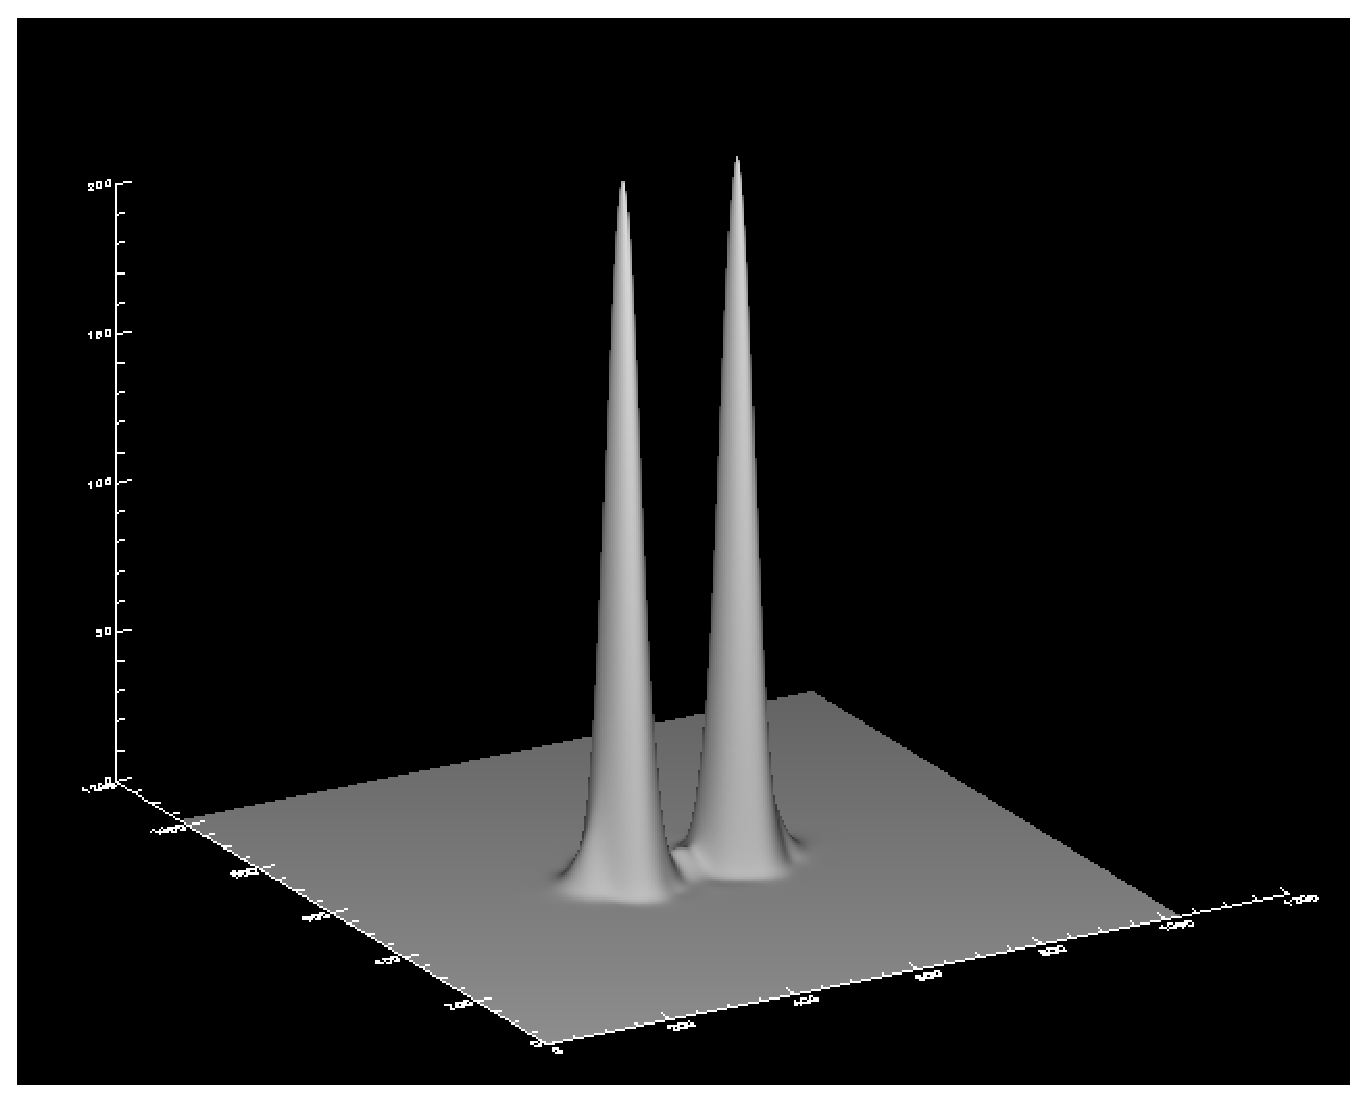
\includegraphics[width=0.49\columnwidth]{./full/twobody/deltas_050}
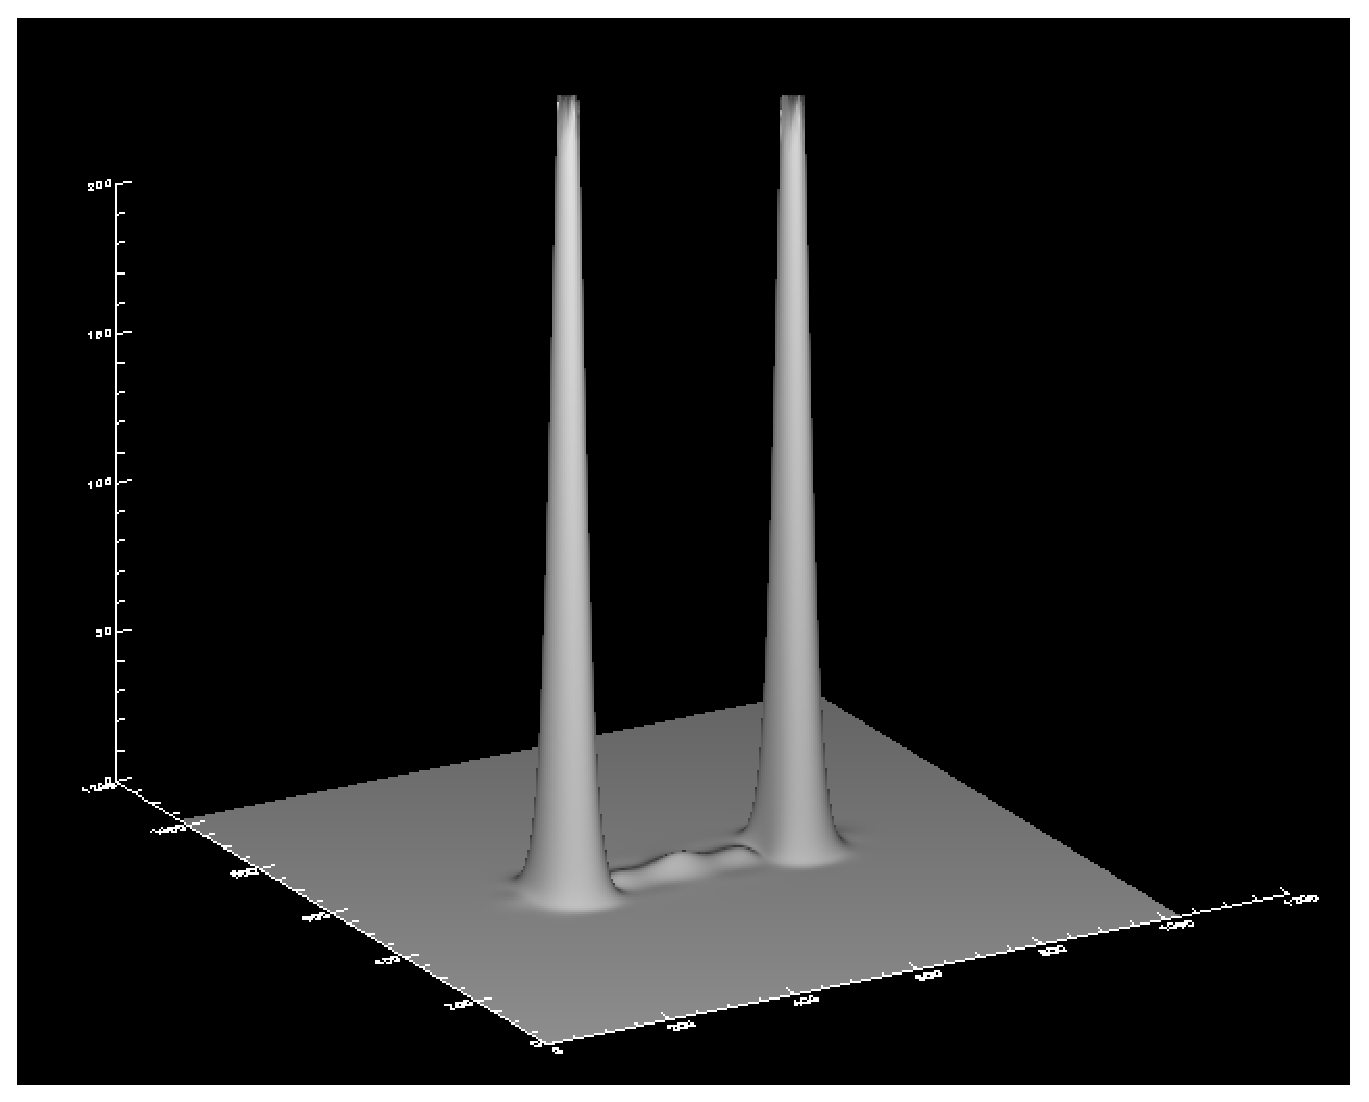
\includegraphics[width=0.49\columnwidth]{./full/twobody/deltas_065}
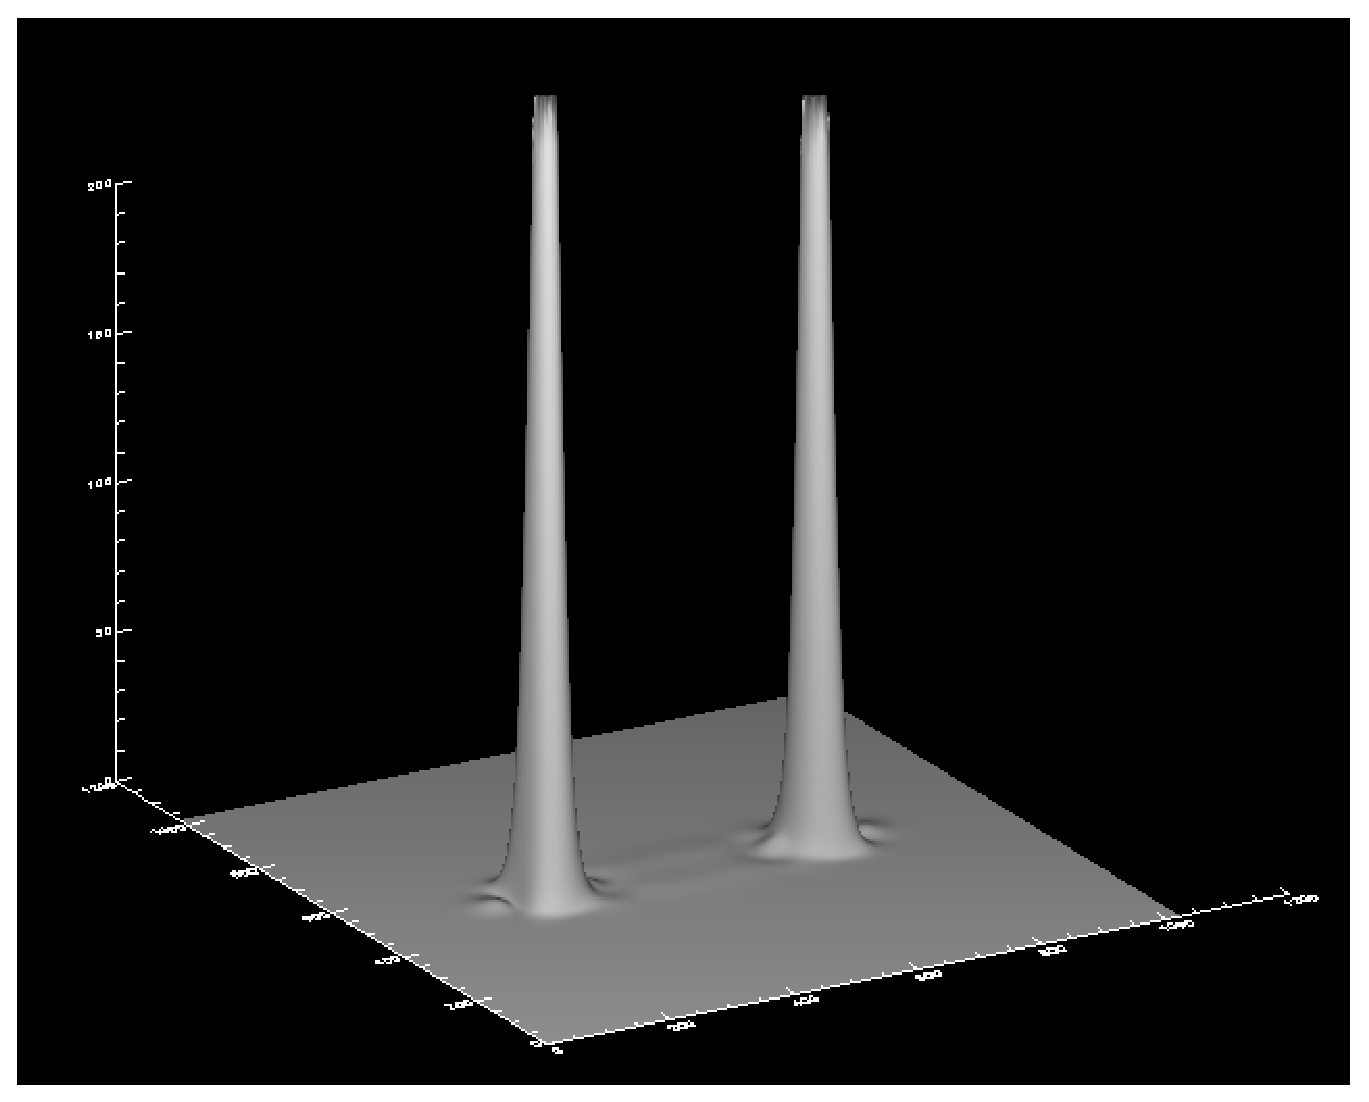
\includegraphics[width=0.49\columnwidth]{./full/twobody/deltas_080}
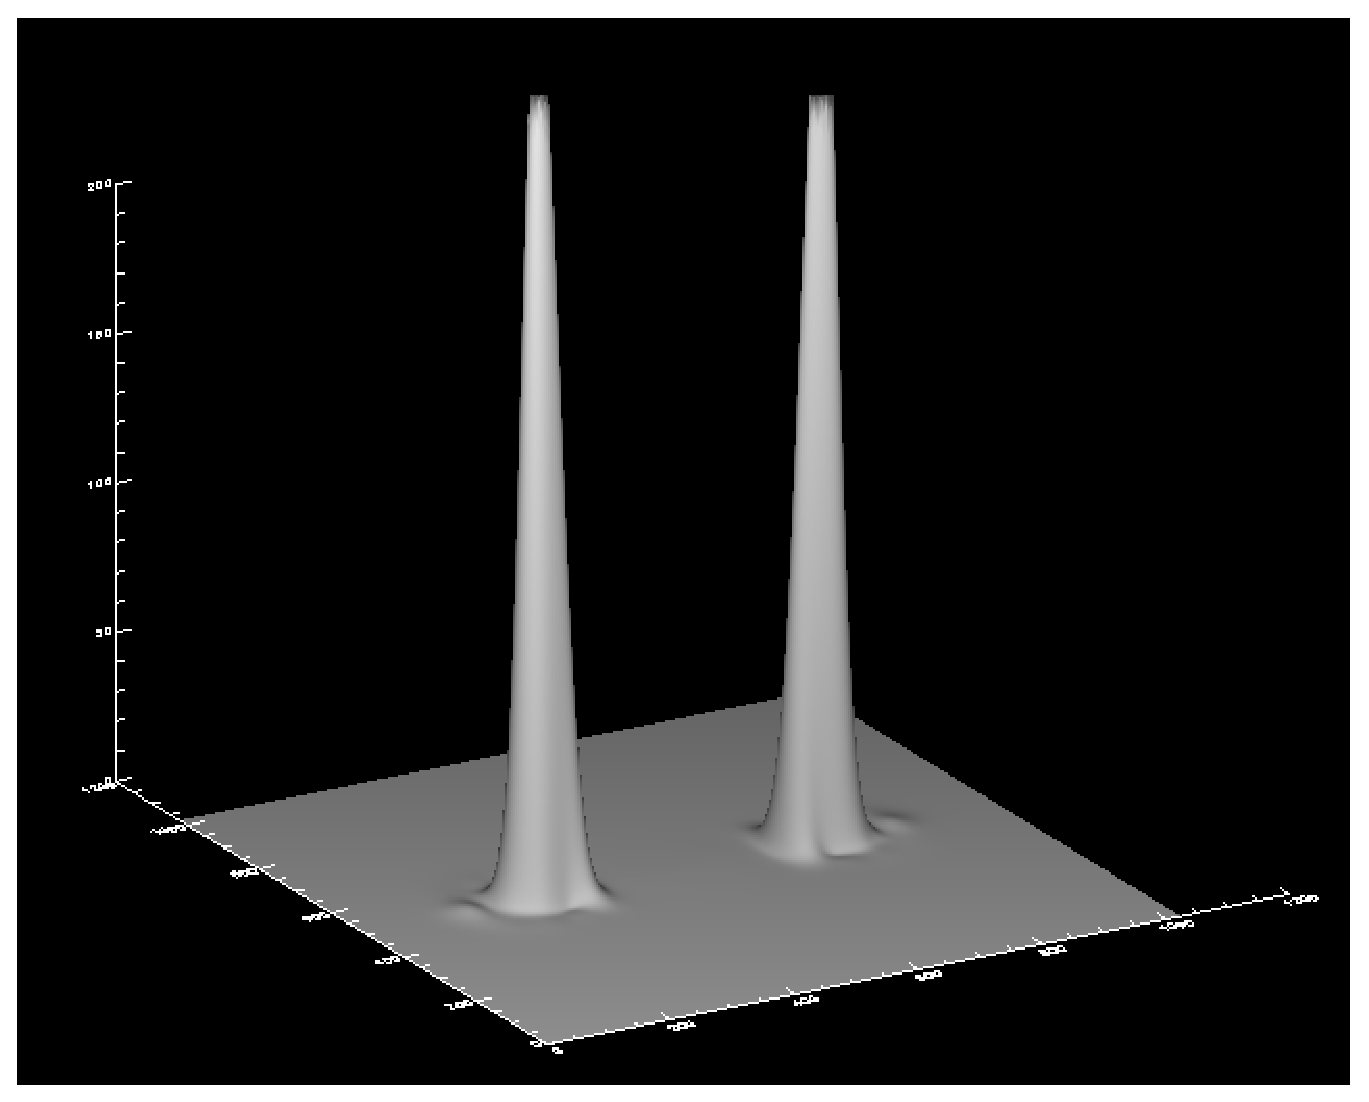
\includegraphics[width=0.49\columnwidth]{./full/twobody/deltas_100}

   \end{center}
\caption{In these plots we can see the two waves pass through each other. The waves collide in the first plot and are then shown to have fully passed through each other in the last plot. The output times are at timesteps of $40, 45, 50, 65, 80, 100$.}
\label{fig.twobody2}
\end{figure}

\begin{figure}[htb]
   \begin{center}
     %\leavevmode
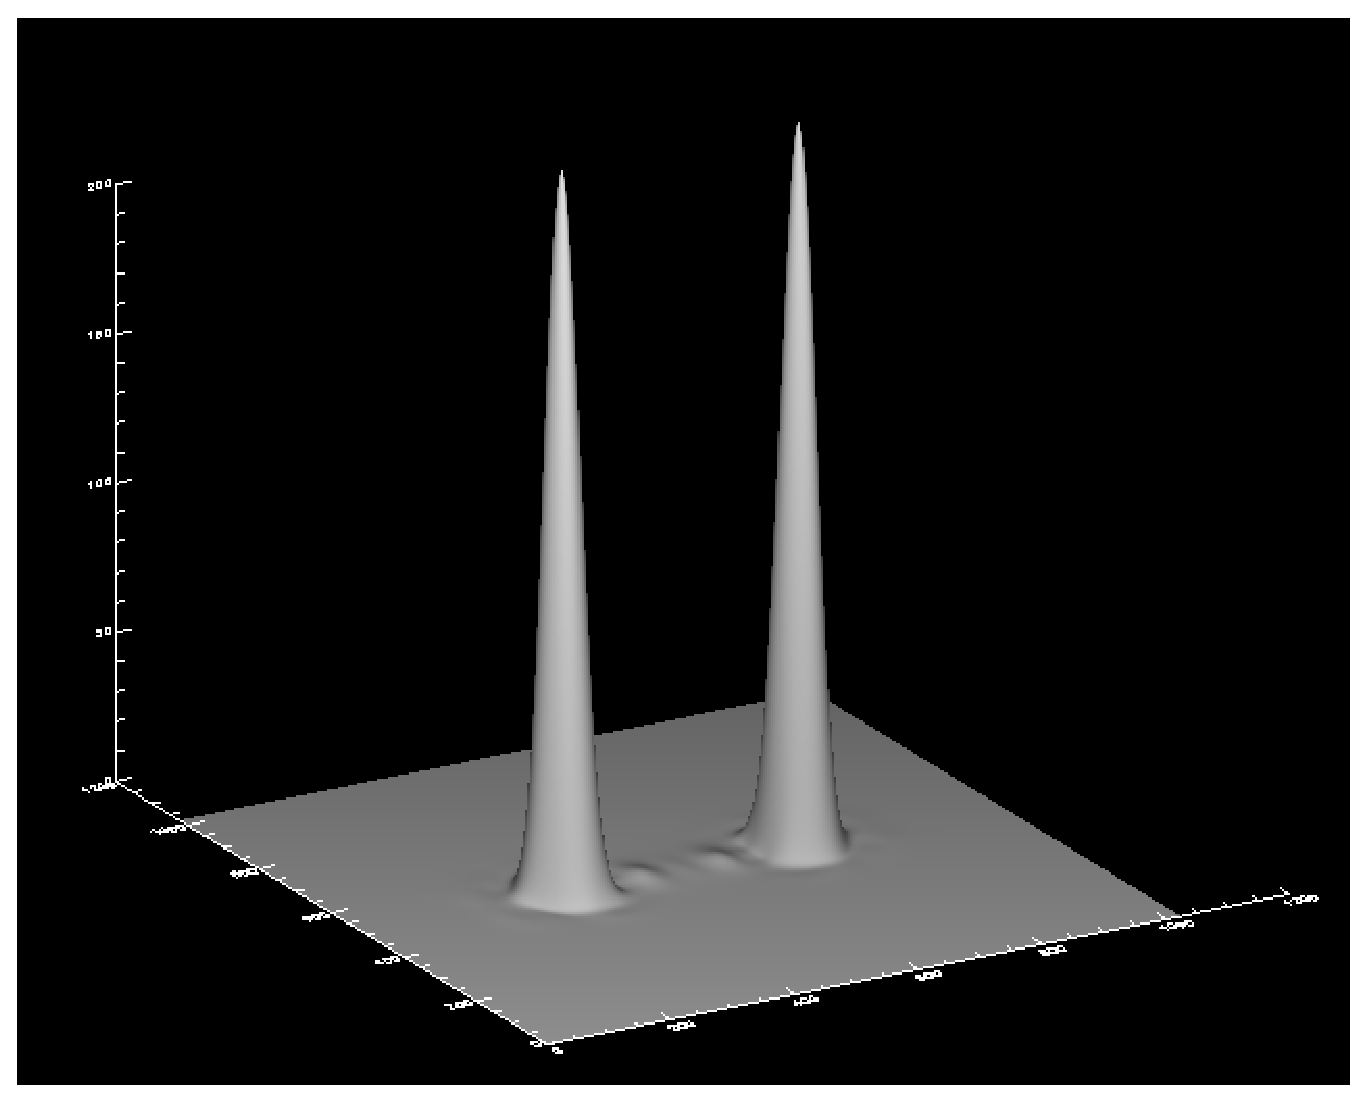
\includegraphics[width=0.45\columnwidth]{./full/twobody/deltas_120}
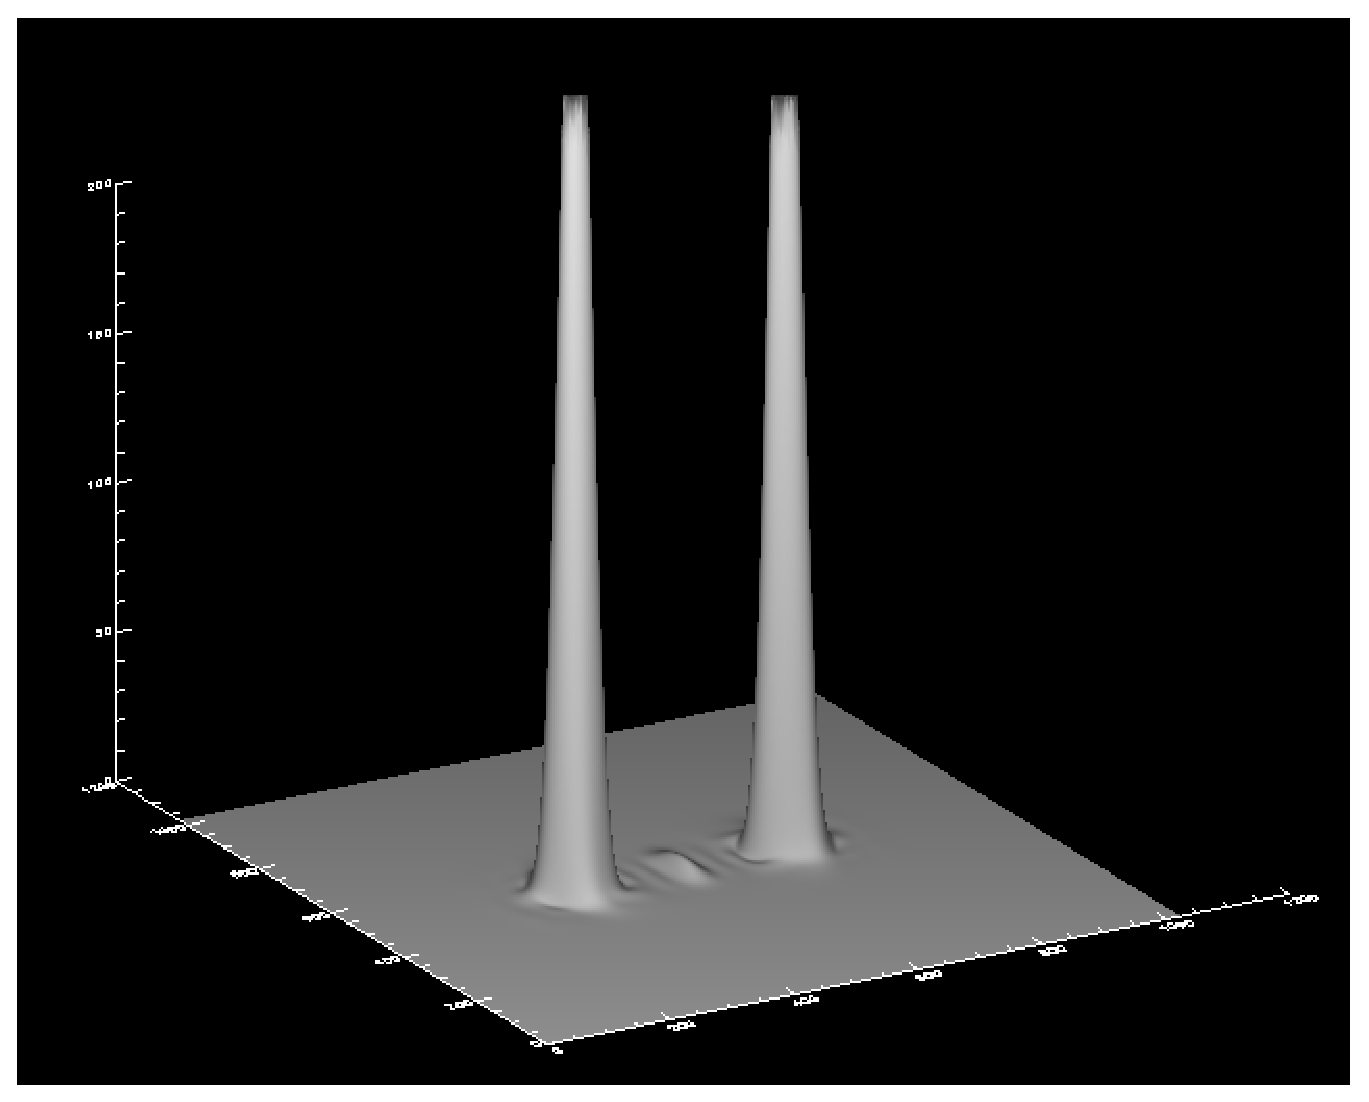
\includegraphics[width=0.45\columnwidth]{./full/twobody/deltas_125}
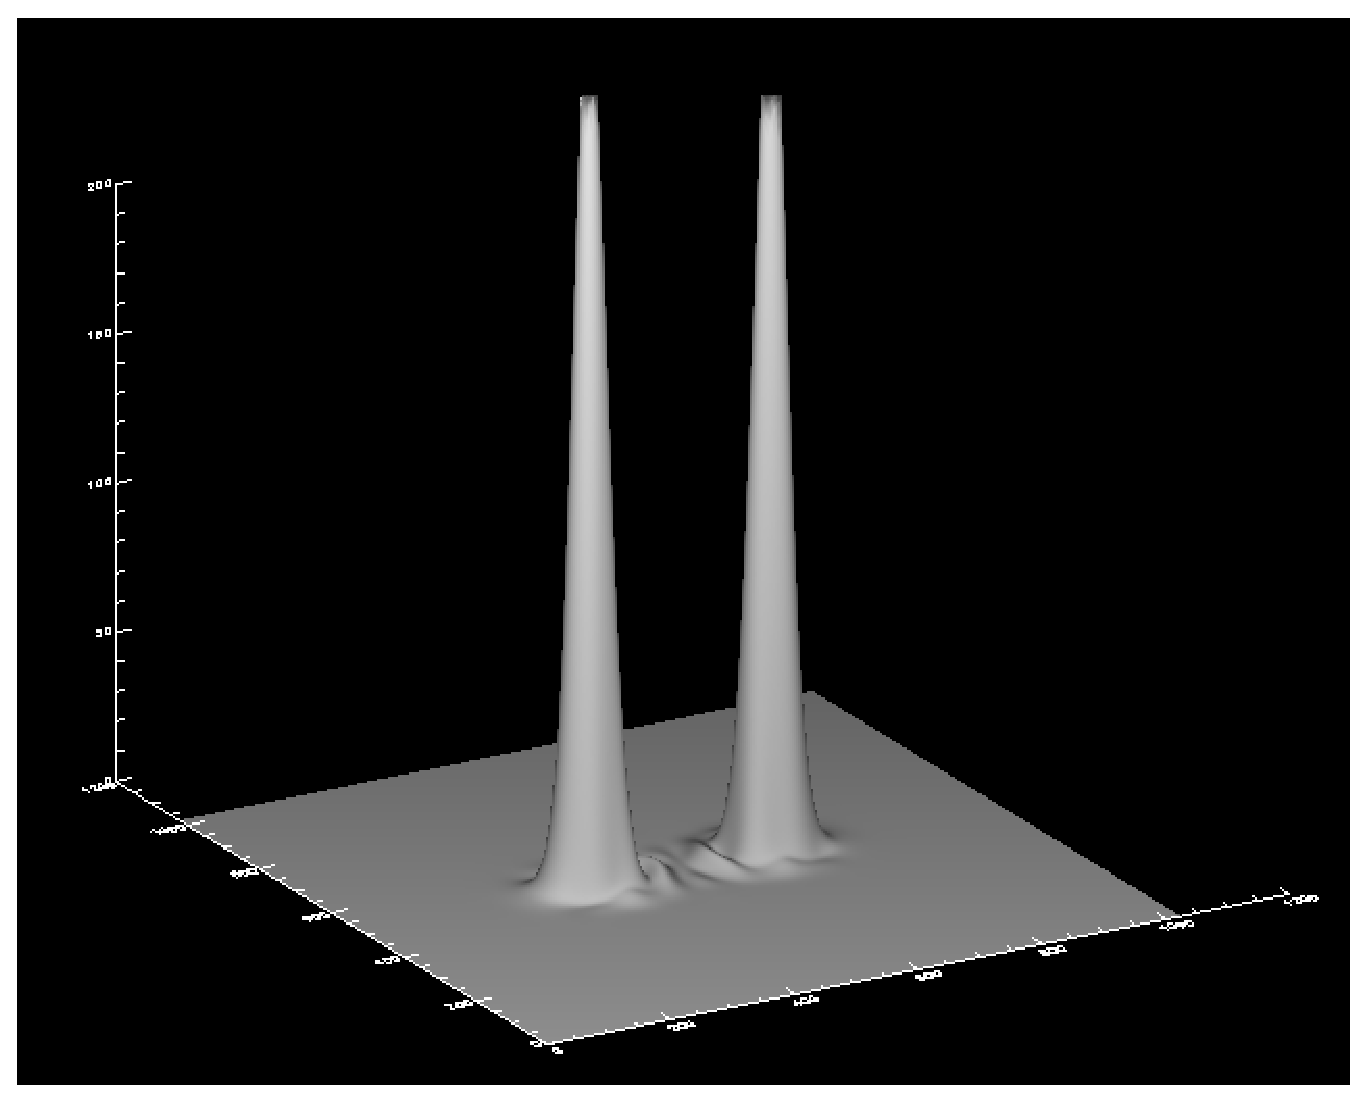
\includegraphics[width=0.45\columnwidth]{./full/twobody/deltas_130}
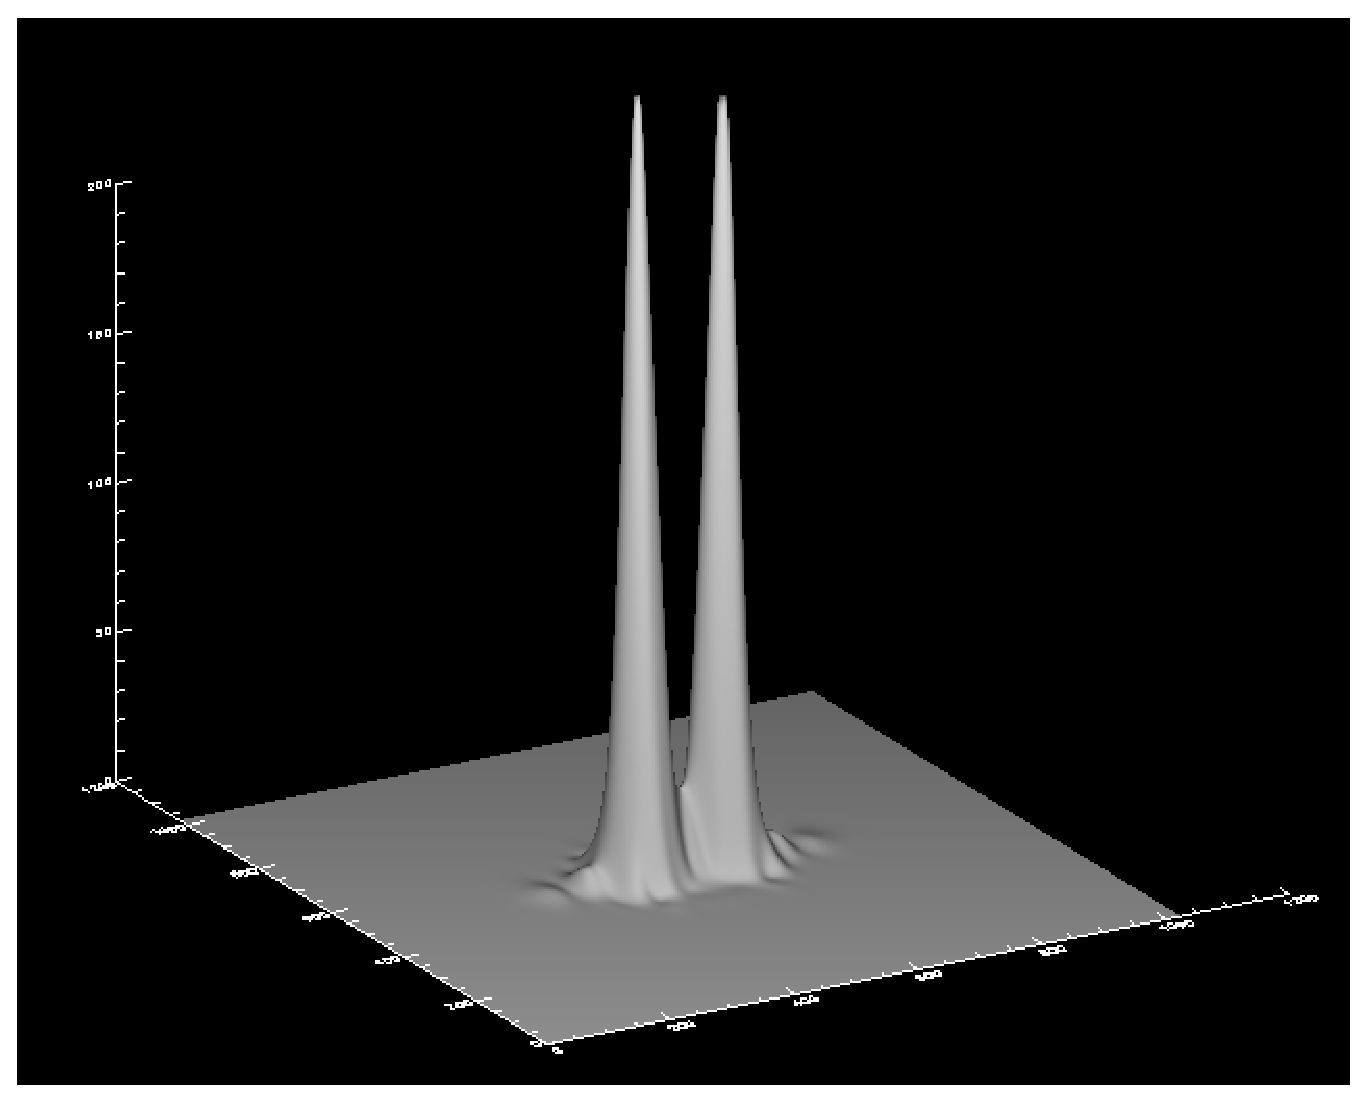
\includegraphics[width=0.45\columnwidth]{./full/twobody/deltas_140}
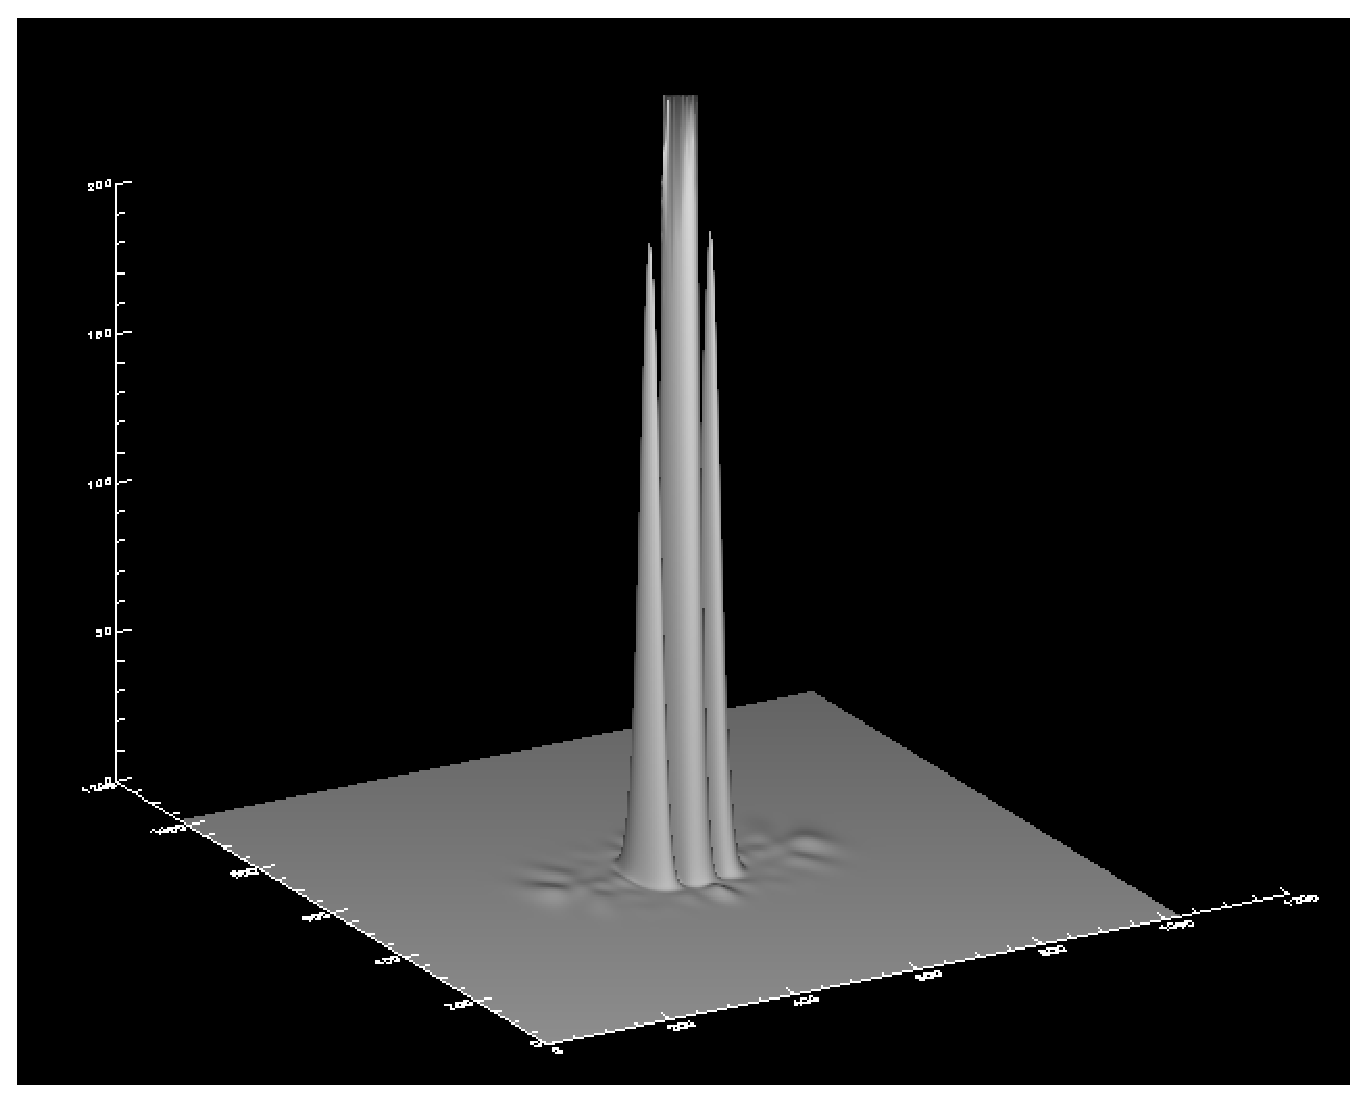
\includegraphics[width=0.45\columnwidth]{./full/twobody/deltas_145}
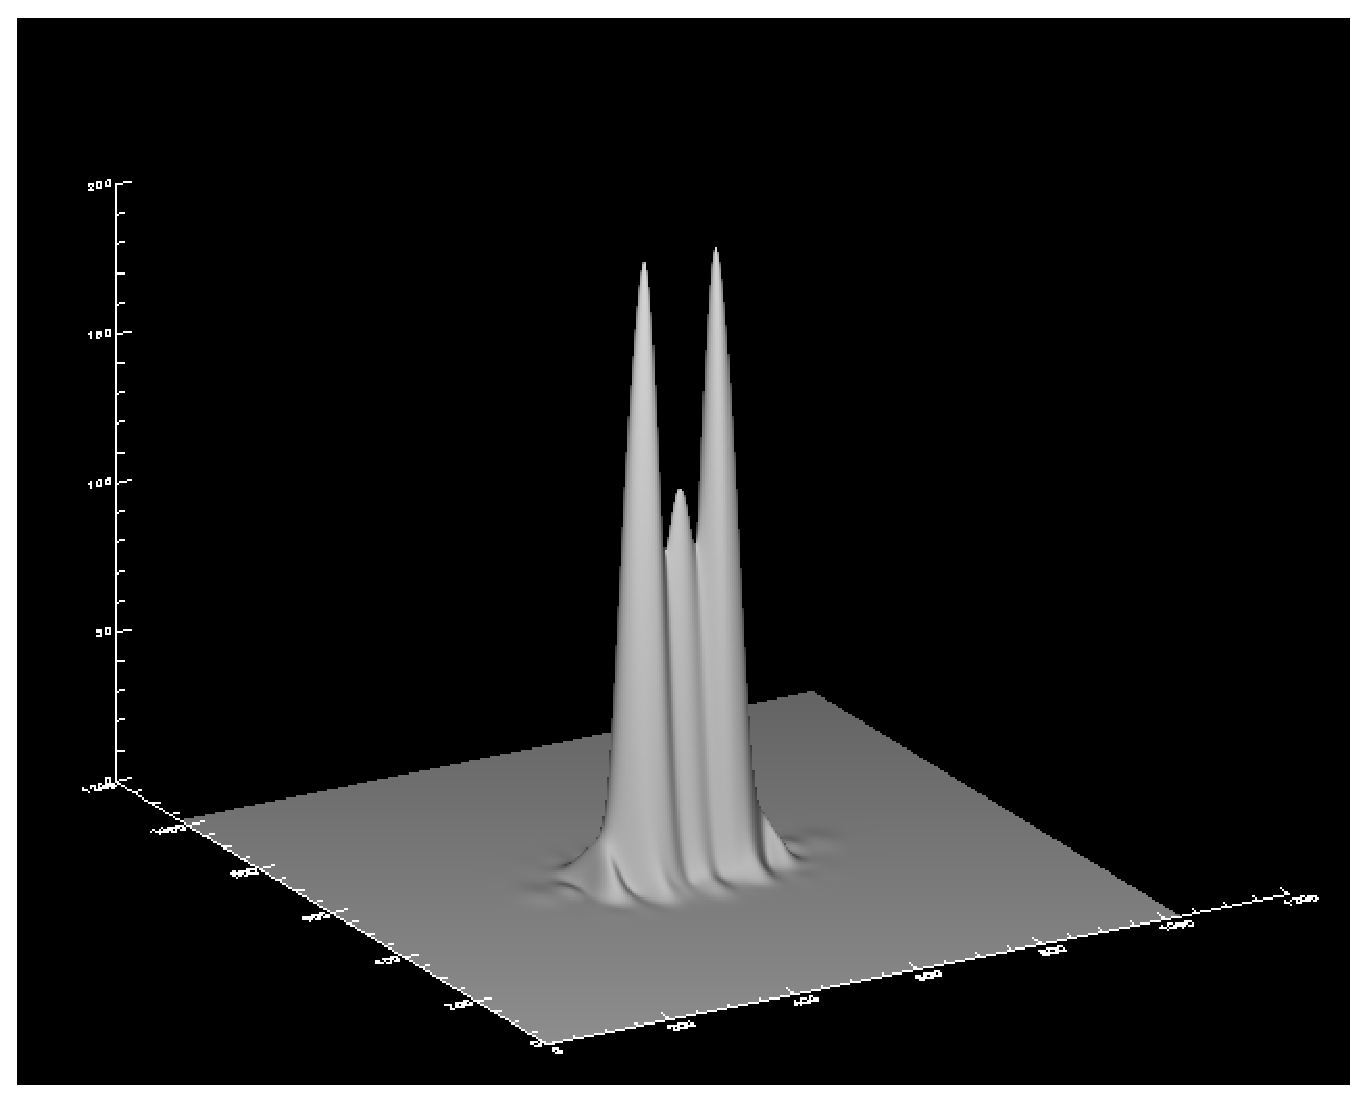
\includegraphics[width=0.45\columnwidth]{./full/twobody/deltas_150}

   \end{center}
\caption{These plots show that after the peaks have passed through each other they will turn around and collapse again. The pattern is similar to before but with some slight differences as noted in results section. The output times are $120, 125, 130, 140, 145, 150$.}
\label{fig.twobody3}
\end{figure}



\subsection{Tophat collapse}
\label{tophat}
The two-body interaction was a test of the gravitational routine, while the test of the tophat collapse will test gravity as well as expansion. Implicitly assumed so far, as in all 3D tests, is the use of splitting operators for implementing wave-mechanics in more than one spatial dimension. The code used here is one that will be used to conduct the full cosmological simulations; hence it is 3D, has periodic boundary conditions, includes self-consistent gravity and cosmological expansion.

The tophat collapse is a classic test of $N$-body codes. Due to the high symmetry of the problem then it is one of the simplest models for analysing non-linear evolution (Coles, \citep{bib_pcoles}). As Coles notes, the tophat is ``not directly relevant to interesting cosmological models because the real fluctuations are expected to be highly irregular and random."

In an $N$-body code then the dynamics will be determined by the cosmological parameters chosen as well as the distribution of the mass. In wave-mechanics there is, as always, one more parameter to consider: the $\nu$ parameter that determines the speed of dispersion as outlined before (section \ref{hydro}). When the mass distribution of the tophat is tall (relative to background density) and thin then collapse will happen more quickly. For a distribution that is short and flat then collapse is suppressed.

The parameters used in this test were: $H_0 = 72, a_i = 0.04, \Omega = 1, \Omega_{m,0} = 0.3, L = 100 {\rm Mpc/h}, \nu = 10^{-8}$. The resolution used is $64^3$ gridpoints where a central over-density that is 8 pixels in diameter and is at a level of $\delta = 2$. See figure \ref{fig.tophat} for the resultant plots.

The results show that the over-density collapses to a nearly singular point by timestep 1800 ($\delta = 6.67$) , the over-density grows until a maximum peak of $\delta = 8.33 $ at timestep 2200. From there it stays at that peak until the end of the simulation (timestep 3200) in an apparently static state.

As point of comparison, we will provide an alternative set of plots (figure \ref{fig.tophat2}) that use a larger value of $\nu$ ($10^{-7}$). This alternative set of plots shows that collapse happens faster, as is expected from using a higher value of $\nu$. The parameters were otherwise held constant, that is to say that we used the same initial conditions. Collapse to the same peak ($\delta = 8.33 $) has now occurred by timestep 800; however, the peak soon drops in height and fattens until the end of the simulation. The over-density is still centralized but it appears that gravity is not strong enough to hold the region as a quasi-singular point of density. In tests where $\nu$ is much larger the over-density expands so fast that the wavefunction crosses over the boundaries. This provides feedback into the system where different frequencies within the wavefunction can cause an interference pattern. The result is an unsmooth wavefunction with rapid variability.


\begin{figure}[htb]
   \begin{center}
     %\leavevmode

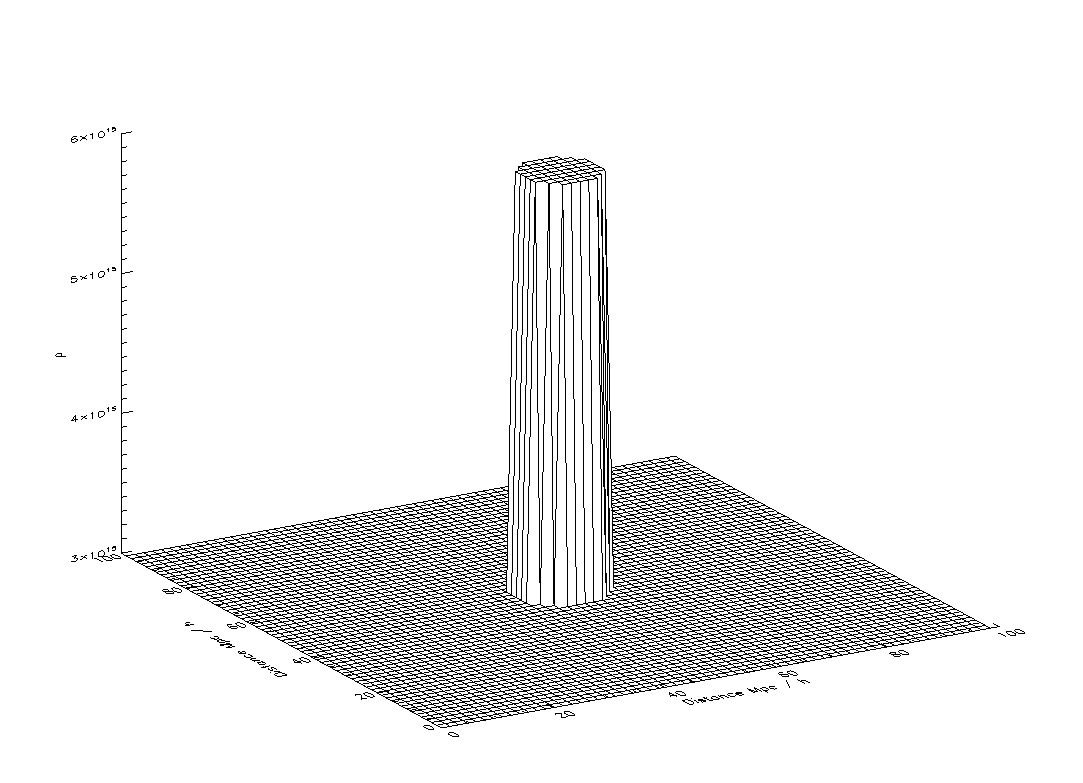
\includegraphics[width=0.49\columnwidth]{./full/tophat/nu_-8--5/tophat.eps}
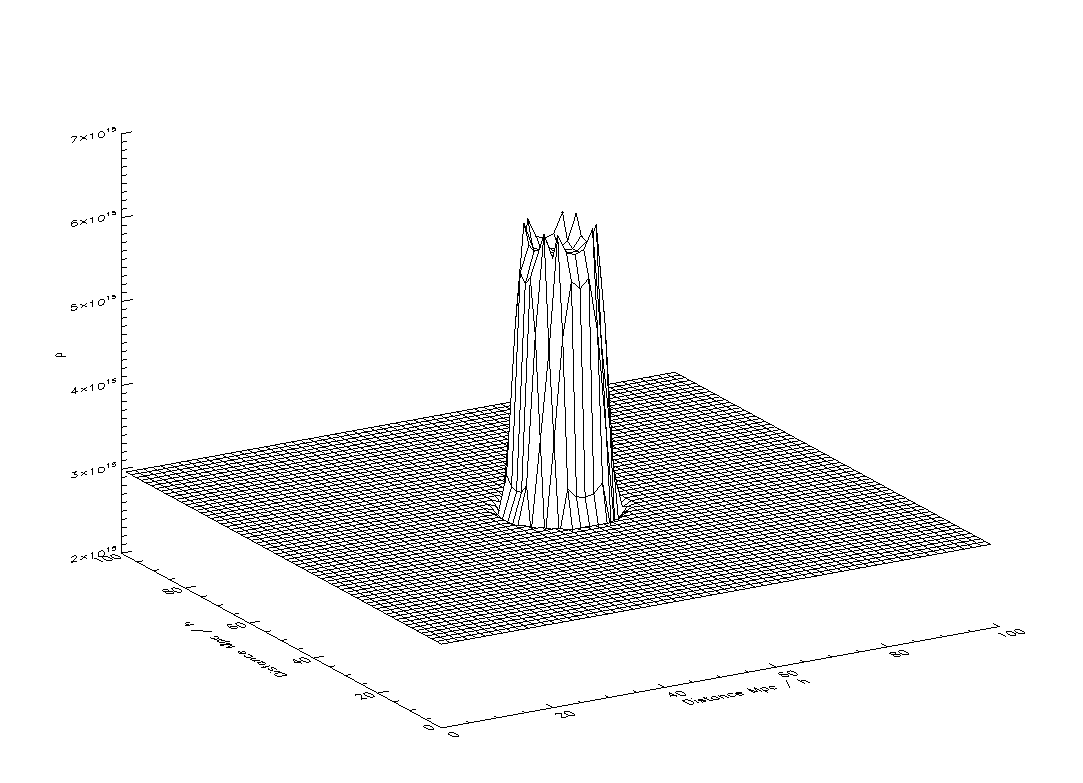
\includegraphics[width=0.49\columnwidth]{./full/tophat/nu_-8--5/rho_evs_00200.eps}

\includegraphics[width=0.49\columnwidth]{./full/tophat/nu_-8--5/rho_evs_00600.eps}

\includegraphics[width=0.49\columnwidth]{./full/tophat/nu_-8--5/rho_evs_1000.eps}

\includegraphics[width=0.49\columnwidth]{./full/tophat/nu_-8--5/rho_evs_2000.eps}

\includegraphics[width=0.49\columnwidth]{./full/tophat/nu_-8--5/rho_evs_3000.eps}
   \end{center}
\caption{The (comoving) plots here show a $2D$ slice of a $3D$ tophat collapse. The top left plot shows the initial condition ($a = 0.04, \delta = 0.1, \nu = 10^{-8}$). The plots (left to right) are $t = 0, 200, 600,$ $1000, 2000, 3000$ ($a= 0.04, 0.05,$ $0.07, 0.1, 0.3, 0.8$).}
\label{fig.tophat}
\end{figure}

\begin{figure}[htb]
   \begin{center}
     %\leavevmode

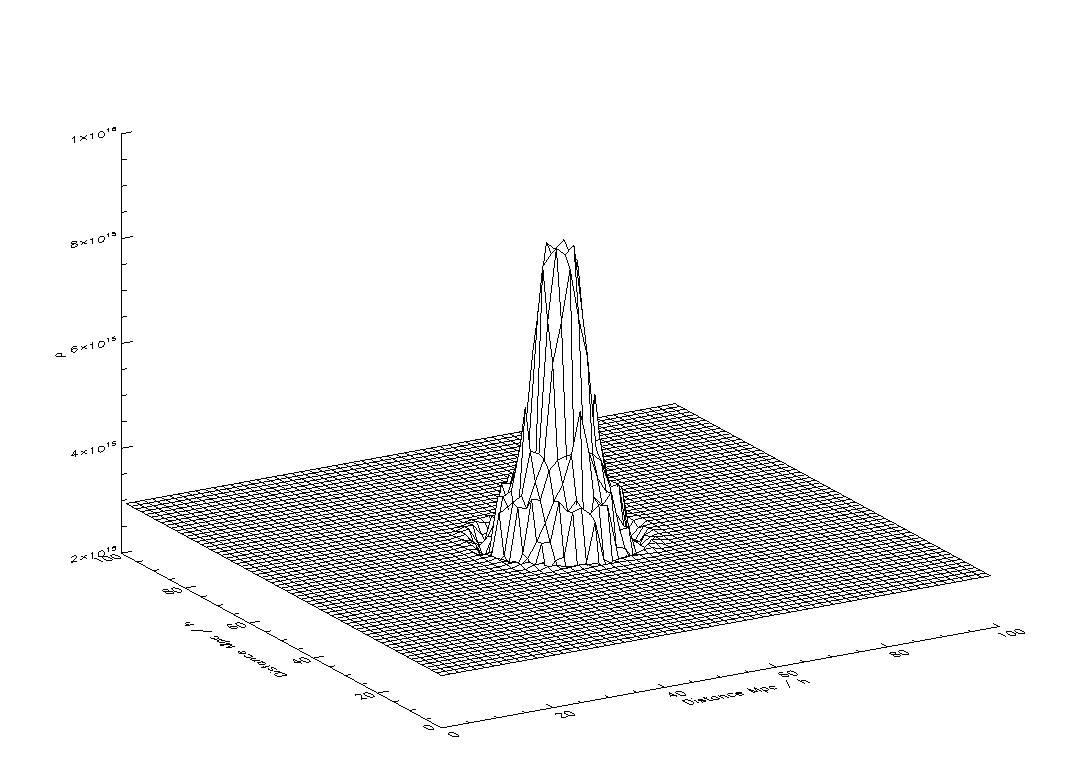
\includegraphics[width=0.49\columnwidth]{./full/tophat/nu_-7/rho_evs_00600.eps}
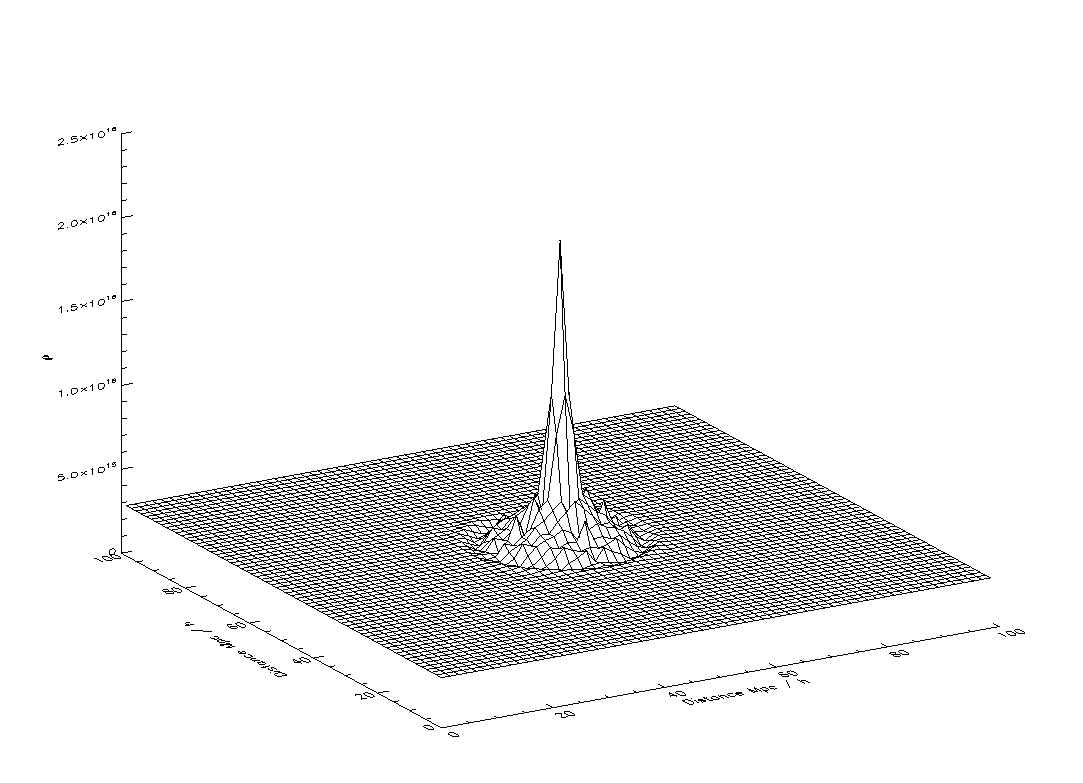
\includegraphics[width=0.49\columnwidth]{./full/tophat/nu_-7/rho_evs_00800.eps}
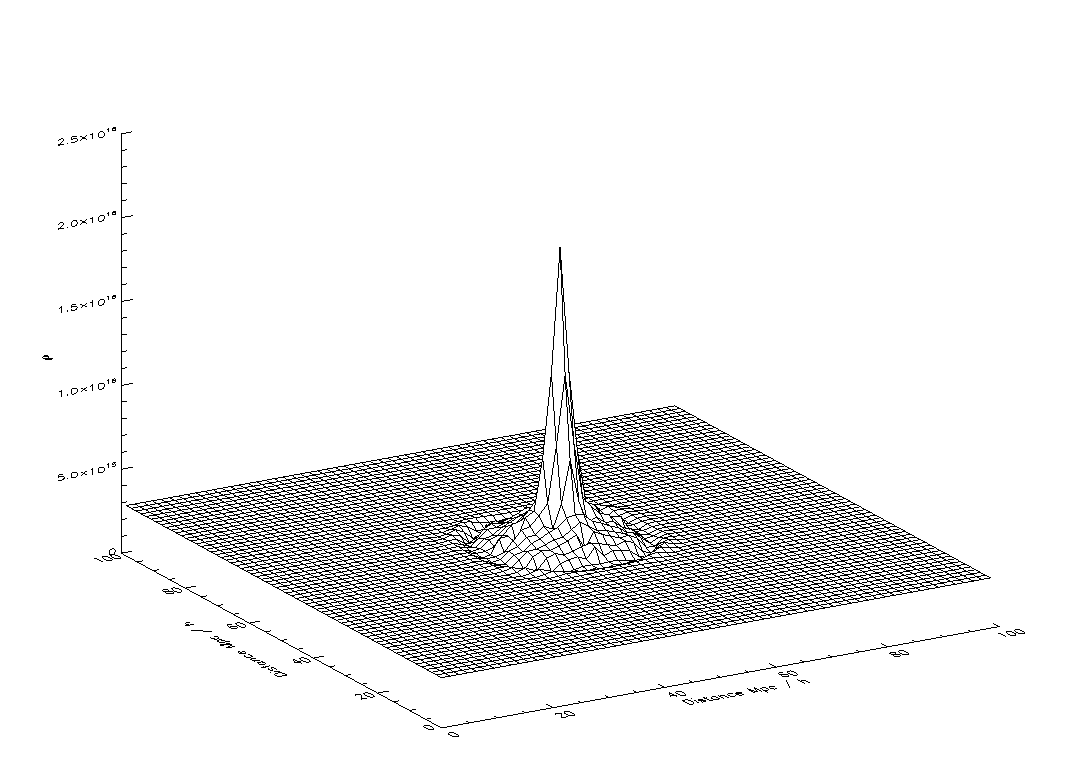
\includegraphics[width=0.49\columnwidth]{./full/tophat/nu_-7/rho_evs_1000.eps}
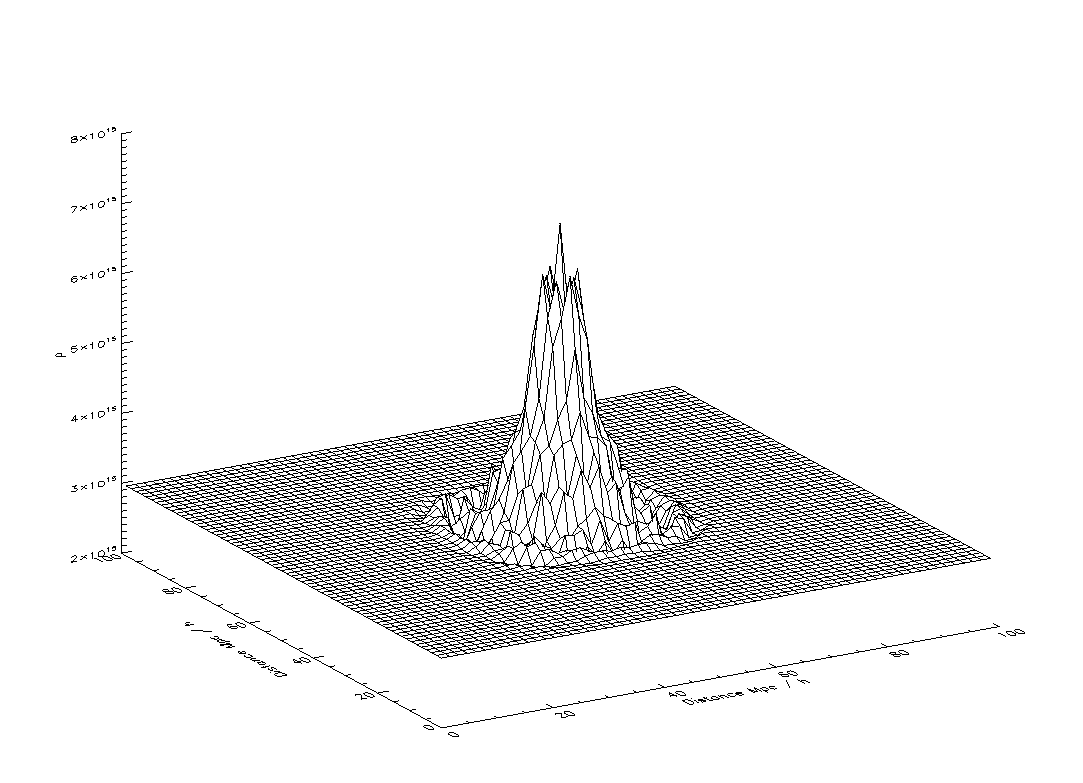
\includegraphics[width=0.49\columnwidth]{./full/tophat/nu_-7/rho_evs_1600.eps}
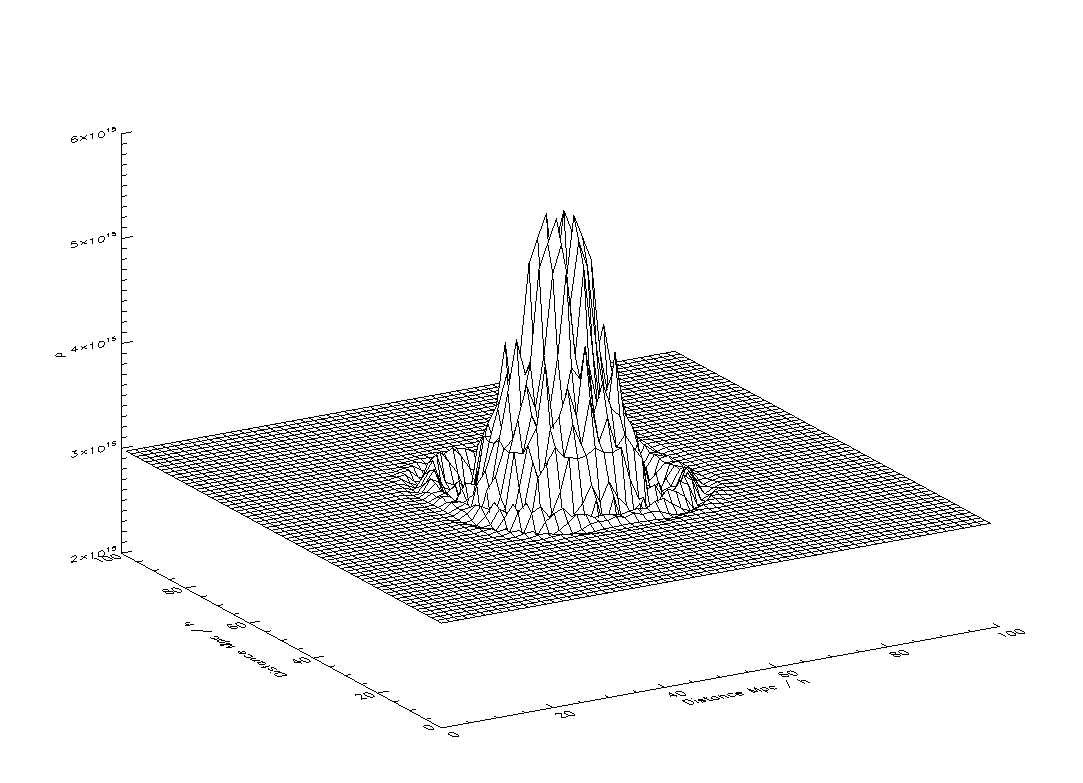
\includegraphics[width=0.49\columnwidth]{./full/tophat/nu_-7/rho_evs_2000.eps}
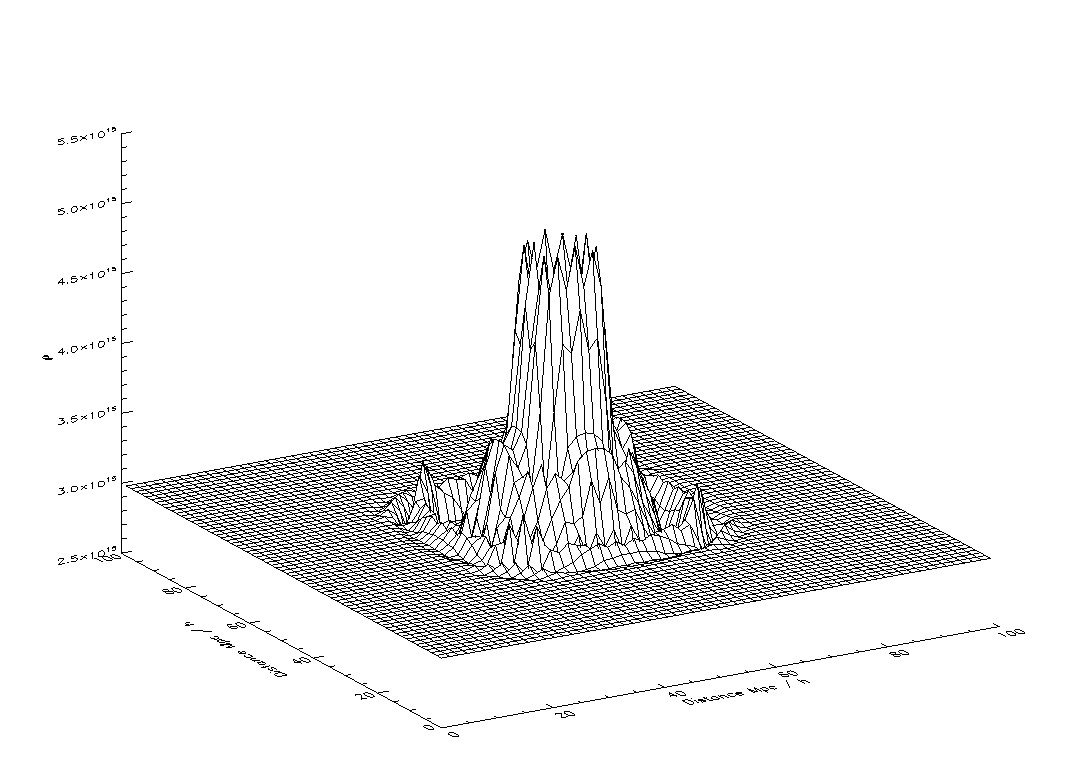
\includegraphics[width=0.49\columnwidth]{./full/tophat/nu_-7/rho_evs_3000.eps}
   \end{center}
\caption{Here is an alternative set of plots of a $3D$ tophat collapse. The top two plots show the initial condition ($a = 0.04, \delta = 0.1, \nu = 10^{-7}$) and the associated gravitational potential. The outputs are at times of $t = 600, 800, 1000, 1600, 2000, 3000$ ($a= 0.07, 0.09, 0.1, 0.19, 0.3, 0.8$).}
\label{fig.tophat2}
\end{figure}


\subsection{Cosmological simulation}
\label{cos_sim}
The key results of this thesis focus upon the application of the 3D code for one set of cosmological parameters, for various mass resolutions ($32^3 - 128^3$). The parameters are appropriate to a flat FLRW Universe and were chosen by Sabiu for his own purposes. Sabiu ran some $N$-body simulations and has donated his initial conditions files (at resolutions of $64^3$ and $128^3$ plus end time outputs for comparison with my wave-mechanics code. He generated initial conditions that were suitable for use with the code GADGET-2. These files include all the key cosmological parameters as well as the positions and velocities of all particles. The details of generating the initial conditions was presented in section \ref{cos_init}.

The process of generating initial conditions appropriate for a wave-mechanics code involves turning the particle positions into a continuous density field. To do this I used the Triangular Shaped Cloud (TSC) routine as provided by the Hydra $N$-body code, this code takes particle positions and outputs the number density. It constructs the density by performing a number count in each cell. This is then multiplied by the critical density of the Universe in order to construct a proper cosmological density field. From the density, a gravitational potential can be calculated using standard Fourier techniques (see \ref{sol_poi}) which is then used to create the initial wavefunction $\psi$. This seems like the fairest way to make a comparison with the industry standard, $N$-body, codes. It is not, however, the only way to create initial conditions.

Woo \& Chiueh \citep{bib_woo, bib_wooc} constructed their initial conditions by assuming the following form: $\psi = 1 + R + I$, where $R, I << 1$. The $R$ and $I$ are the real and imaginary perturbations about the mean value ($ = 1$) of the wavefunction. These perturbations are supposed to form a gaussian random field as required by cosmological structure theory. Such a method is attractive as if it can be done in a manner that faithfully represents a ``cosmological wavefunction" then it would avoid the necessity of smoothing particle positions. Performing this smoothing operation will inherently introduce error into the system as the particles positions were originally populated within an underlying smooth density field. Simply smoothing the positions will not give a completely faithful representation of the original field. An alternative possibility and perhaps the simplest approach would be to take the initially continuous density field from an initial condition generator (before one populates it with particles) and use that to construct the wavefunction.

Sabiu generated his initial conditions using the following parameters: $a = 0.03125,$ $\Omega_{m,0} = 0.279, \Omega_{\Lambda,0} = 0.721, \Omega_{b,0} = 0.04554, H_0 = 70.1, {\rm Box \; size} = 500 {\rm Mpc \; h^{-1}}$. Box size is the side length of the box in physical units. This corresponds to a system of physical units where one computational unit of length is $3.08568\times 10^{24}$ cm, one unit of mass is $1.98892\times 10^{43}$ g and the unit of velocity is $100000$ cm / s.

After running the TSC routine to compute density for the initial conditions, a further calculation was performed to construct the over-density field. This was done for all subsequent outputs too. The maximum and minimum over-density in the initial condition were $|\delta| \sim 0.3 $. The simulations at resolutions of $32^3$ and $64^3$ prove to be unsatisfactory as the magnitude of $\delta$ appears to be too high (this could be a problem of conversion from the discrete particle distribution, a simple yet crude solution is to smooth the data). The simulations are unreliable because the maximum value of $\delta$ grows too quickly: from a value of $\sim 0.3$ to $\sim 6$ after only a few hundred timesteps (compare this to an end time of 3500 timesteps $\sim a = 1$).

Figure \ref{fig.dc_problem} shows this problem from the results of a $64^3$ simulation. Manipulating the value of $\nu$ is not sufficient to give reliable results, collapse either comes too fast or not at all.

\begin{figure}[htb]
   \begin{center}
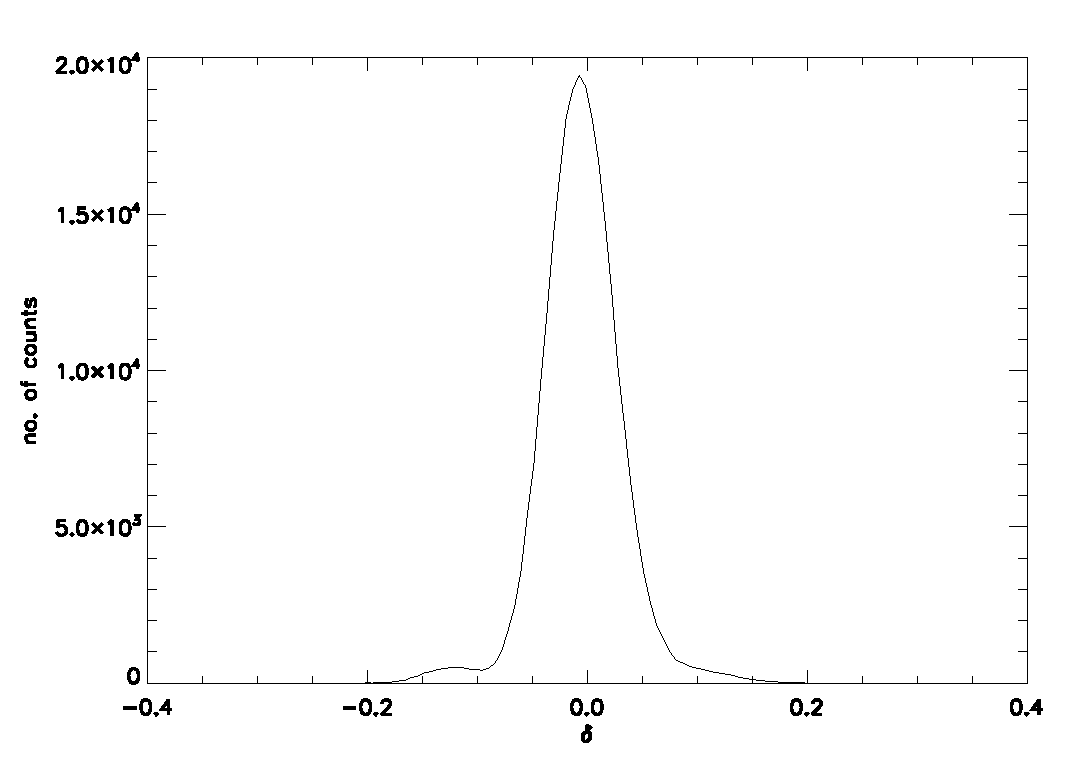
\includegraphics[width=0.49\columnwidth]{./full/wm64/hist/old/psi_r0_hist_dc}
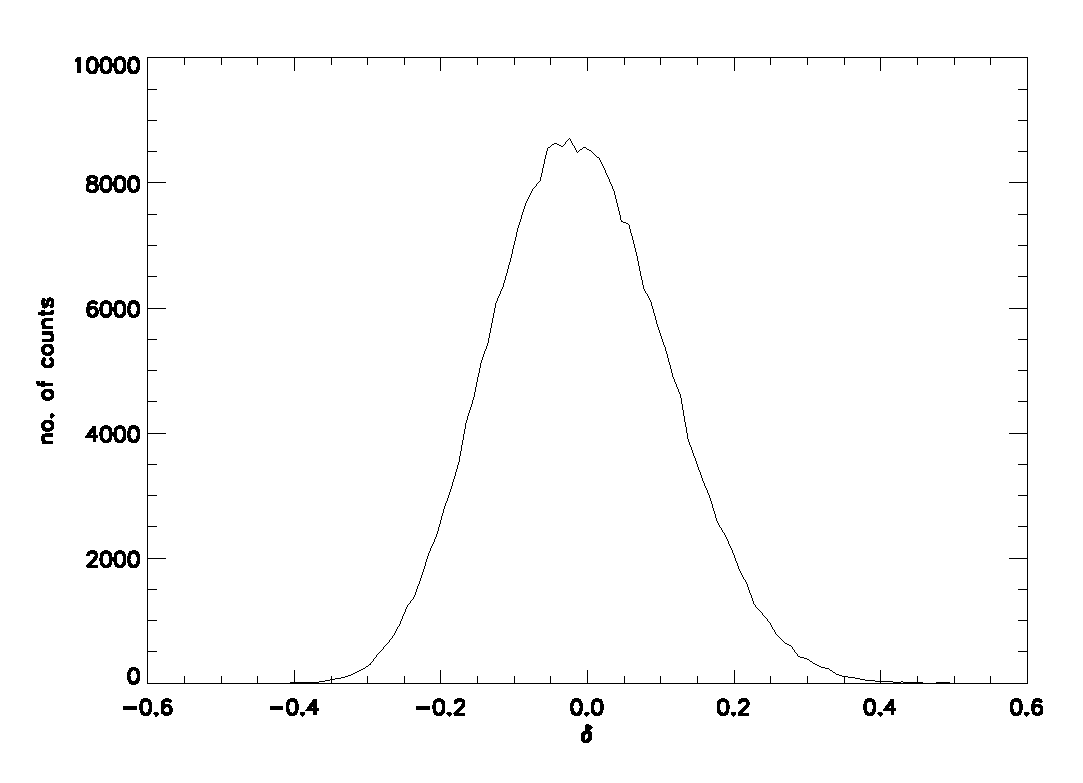
\includegraphics[width=0.49\columnwidth]{./full/wm64/hist/old/psi_r10_hist_dc}
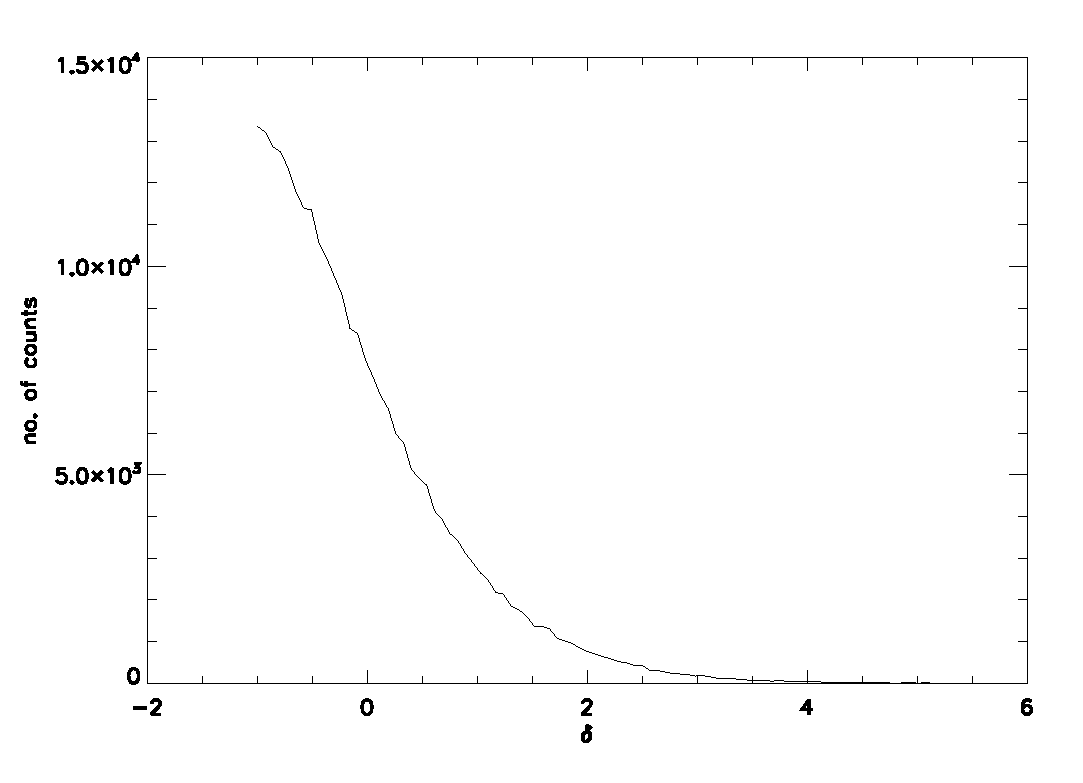
\includegraphics[width=0.49\columnwidth]{./full/wm64/hist/old/psi_r100_hist_dc}
   \end{center}
\caption{These plots show histograms of over-density as generated from the wave-mechanics code. The outputs are for timesteps = 0, 10, 100. This corresponds to $a = 0.03125, 0.0315, 0.0345$. The maximum over-density in the final plot $\delta \sim 6$ is much higher than is expected from present structure formation theory.}
\label{fig.dc_problem}
\end{figure}

Simulations of higher resolution (such as $128^3$) do not seem to suffer from the same problem: the increase in $\delta_{max}$ is more gradual. This suggests that resolutions of $64^3$ and below are just too rough for our implementation of wave-mechanics; however, we believe this problem can be resolved. We suspect the problem is to do with the initial density field generated by the TSC routine. If we take an initial field and decrease the initial magnitude of $\delta$ such that the new field is $\delta' = \delta / 10$ then the increase in the over-density is more gradual (as expected).

Before running the wave-mechanics simulation we checked the Gadget files (initial and late times) to see if they were what we expected (that is, the results produce the behaviour we expected). One such test is to create histograms of the density ($\rho$) and the over-density ($\delta$) fields. The histogram of density should be gaussian in shape and show an increase in width over time. The highest density reached in each output is higher than the previous output, indicating that dense regions are accreting more material and collapsing under the force of gravity. The under dense regions are losing more mass over time (the material is attracted away from these regions in the higher density regions), hence the troughs of the density are lower with each output. The histogram at later times are also gaussian. They are plotted in figure \ref{fig.gadhist} and come from a $64^3$ simulation.

The behaviour of the over-density fields (from Gadget) corroborates with the behaviour of the density field. The histogram of over-density is initially gaussian but tends towards a log-normal in later outputs as seen in figure \ref{fig.gadhistdc}. The initial density field is smooth where deviations from the mean density are small, as indicated by the tight distribution in the first histogram of over-density (a standard deviation of about 0.02). The over-density field is skewed as the minimum value (by definition) is -1 while the maximum can increase (almost) without bound.

\begin{figure}[htb]
   \begin{center}
     %\leavevmode..

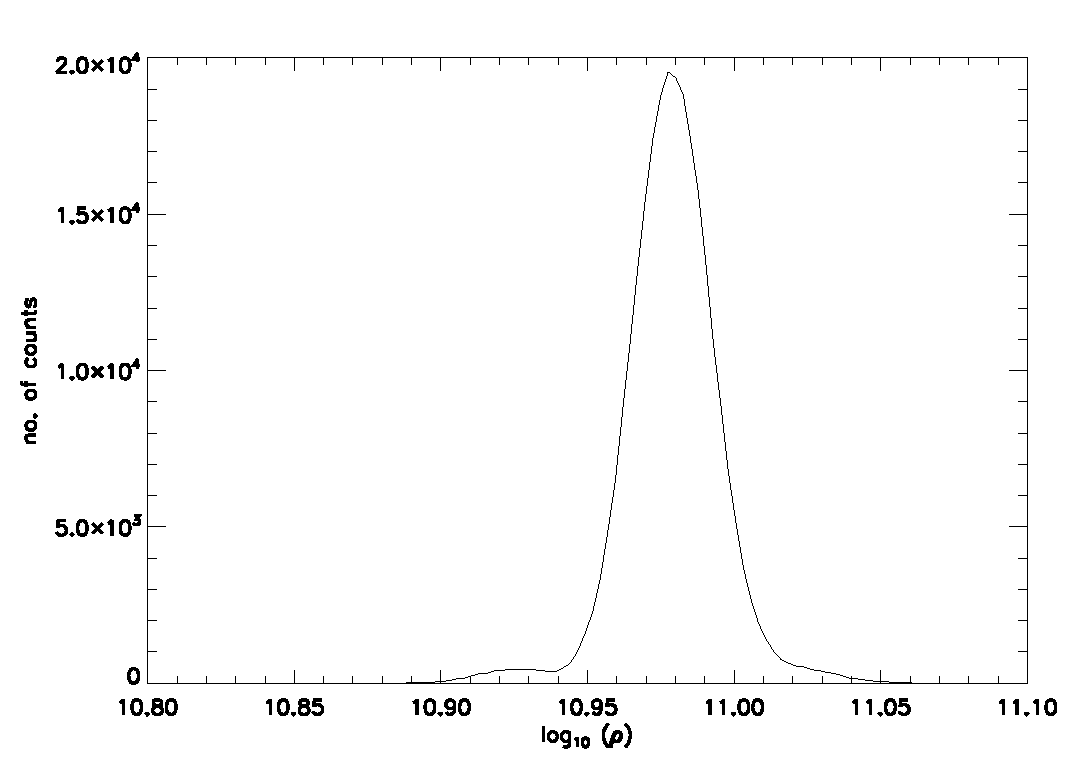
\includegraphics[width=0.49\columnwidth]{./full/gadget/hist_0000}
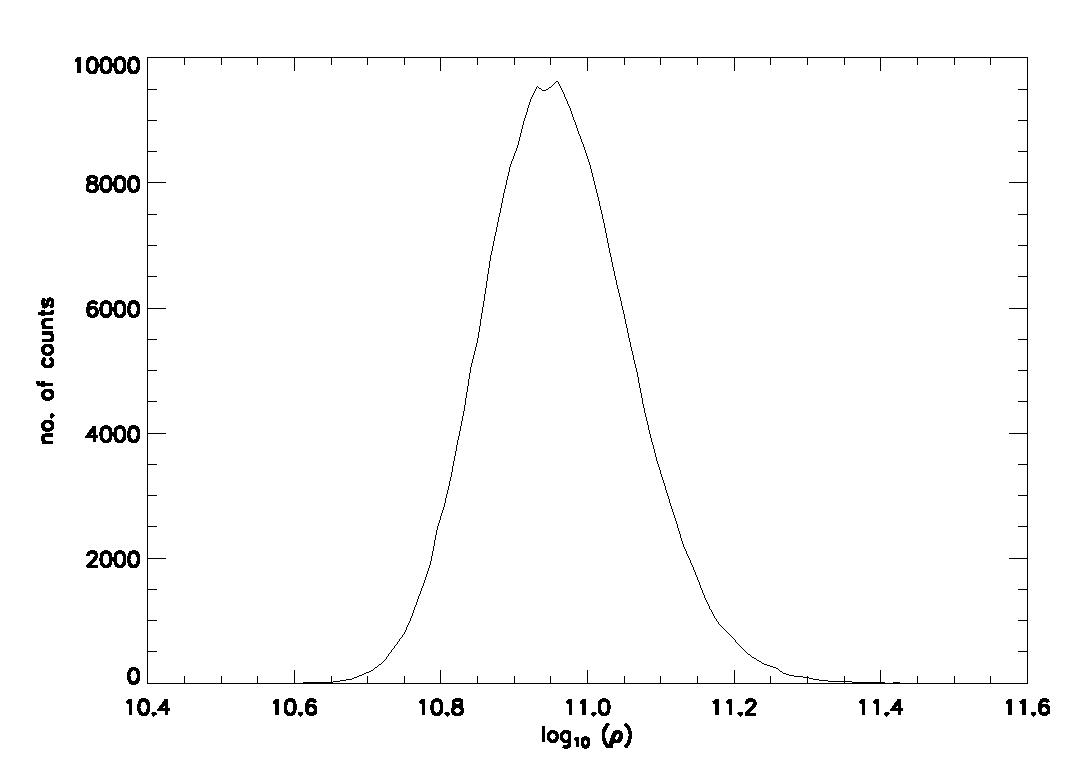
\includegraphics[width=0.49\columnwidth]{./full/gadget/hist_000}
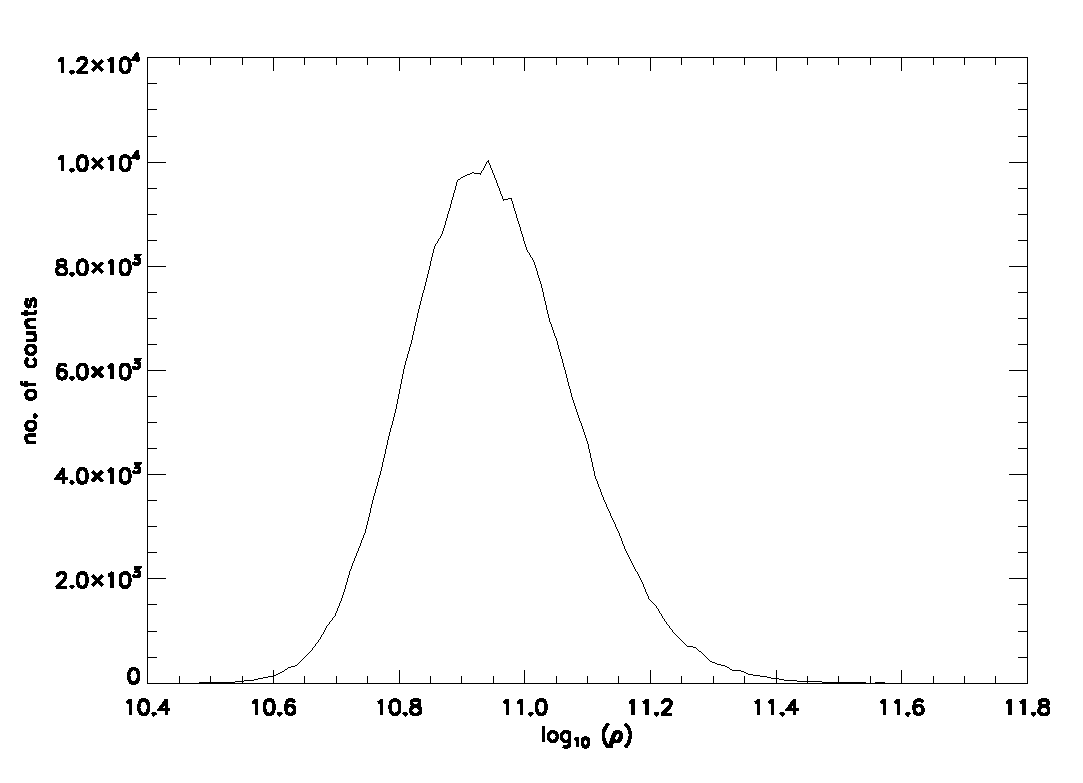
\includegraphics[width=0.49\columnwidth]{./full/gadget/hist_001}
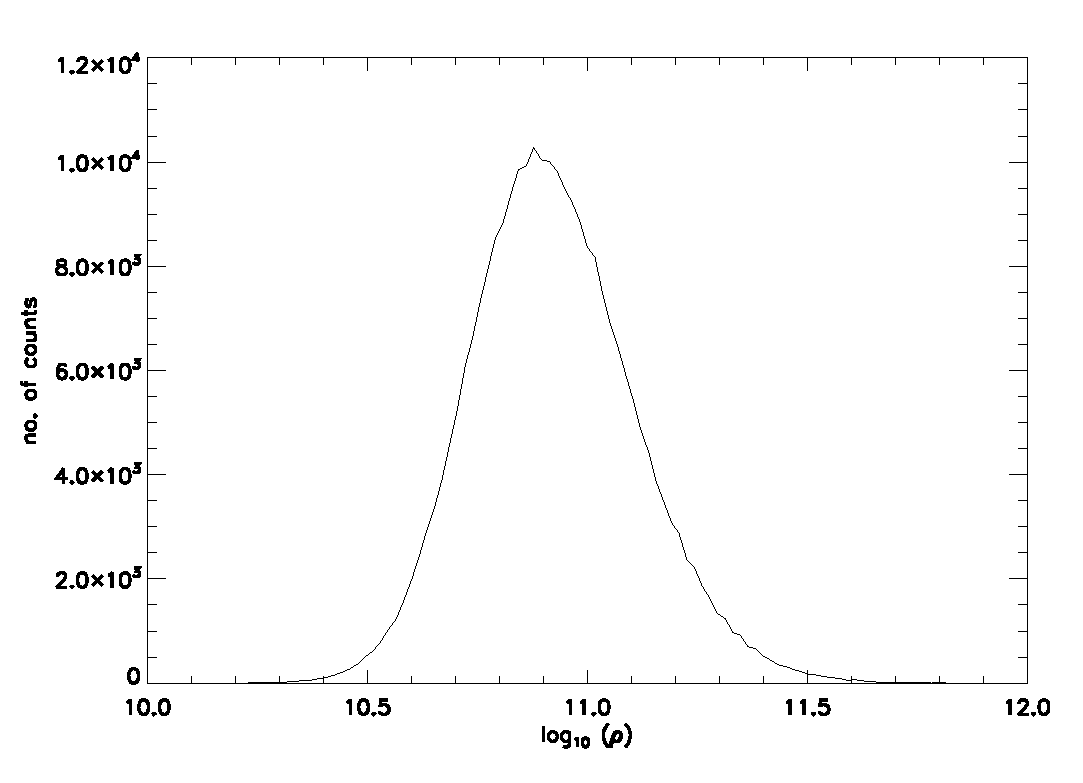
\includegraphics[width=0.49\columnwidth]{./full/gadget/hist_002}
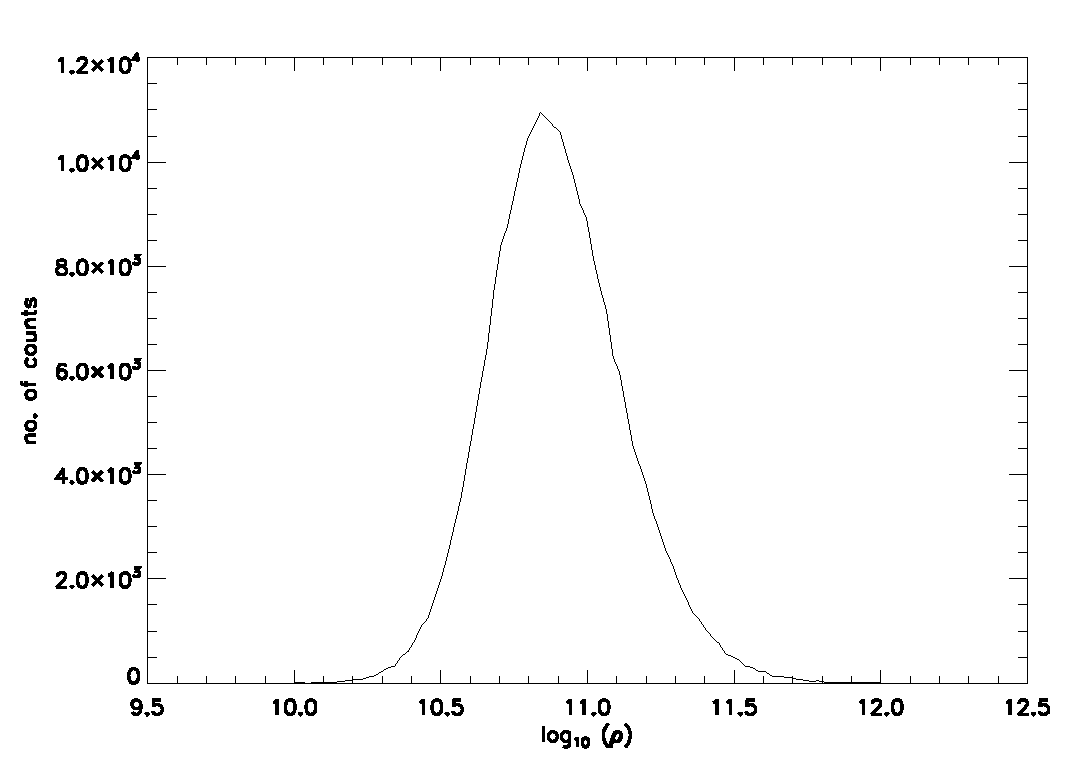
\includegraphics[width=0.49\columnwidth]{./full/gadget/hist_003}
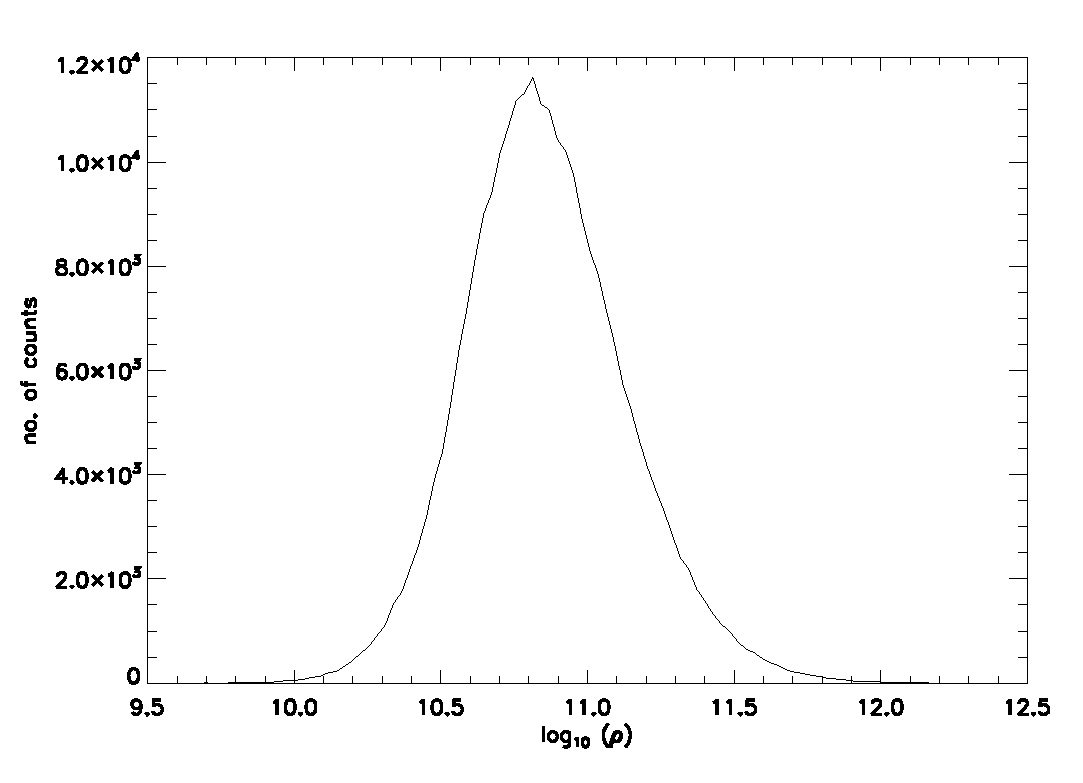
\includegraphics[width=0.49\columnwidth]{./full/gadget/hist_004}

   \end{center}
\caption{These plots show histograms of density as generated from the Gadget outputs. They have a distinctly gaussian shape and widen over time. The outputs are for $z = 32, 3, 2, 1, 0.5, 0.05.$}
\label{fig.gadhist}
\end{figure}

\begin{figure}[htb]
   \begin{center}
    % \leavevmode

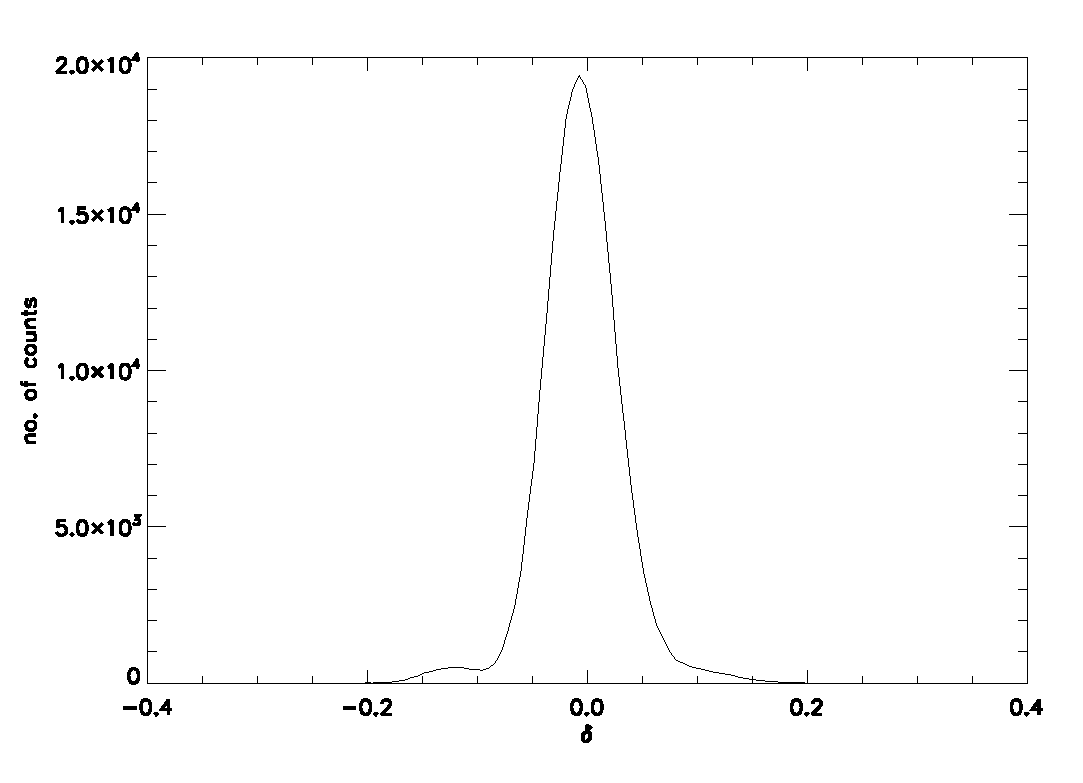
\includegraphics[width=0.49\columnwidth]{./full/gadget/hist_delta_0000}
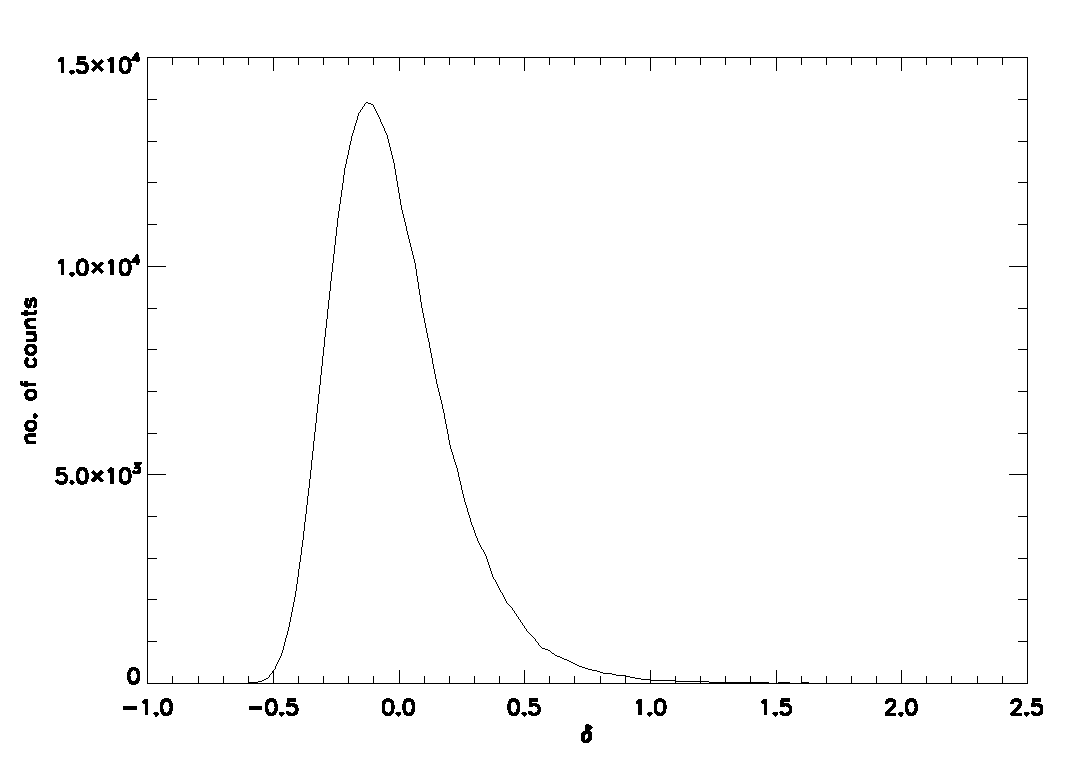
\includegraphics[width=0.49\columnwidth]{./full/gadget/hist_delta_000}
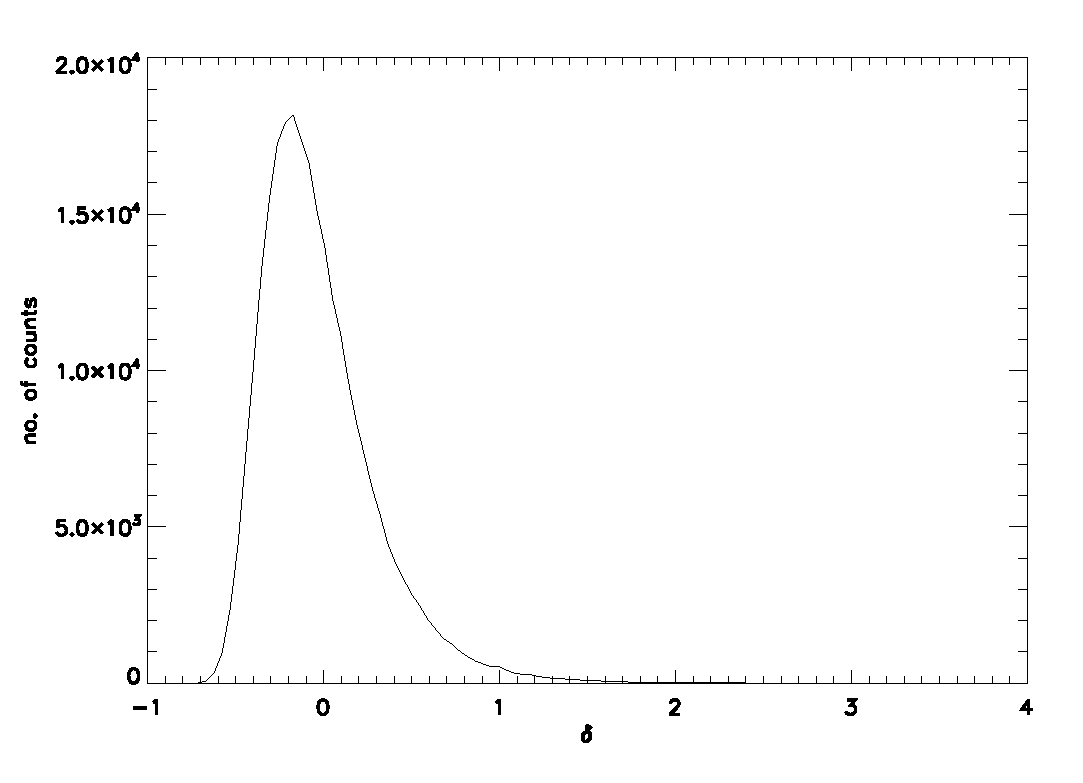
\includegraphics[width=0.49\columnwidth]{./full/gadget/hist_delta_001}
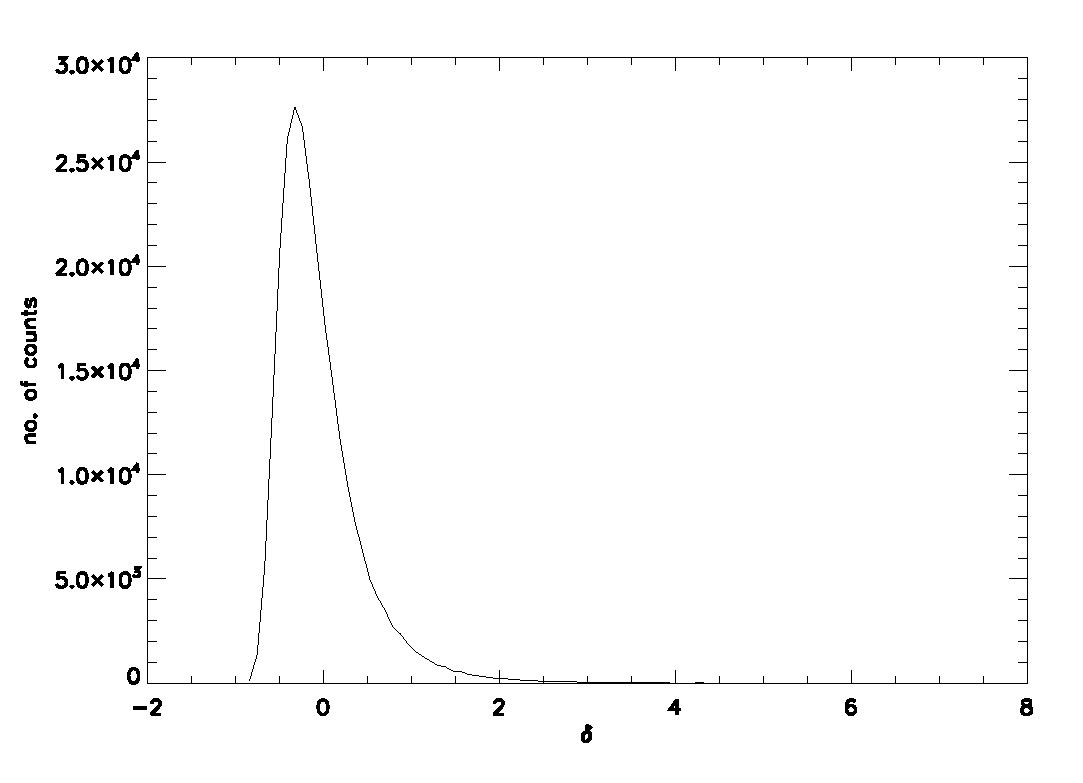
\includegraphics[width=0.49\columnwidth]{./full/gadget/hist_delta_002}
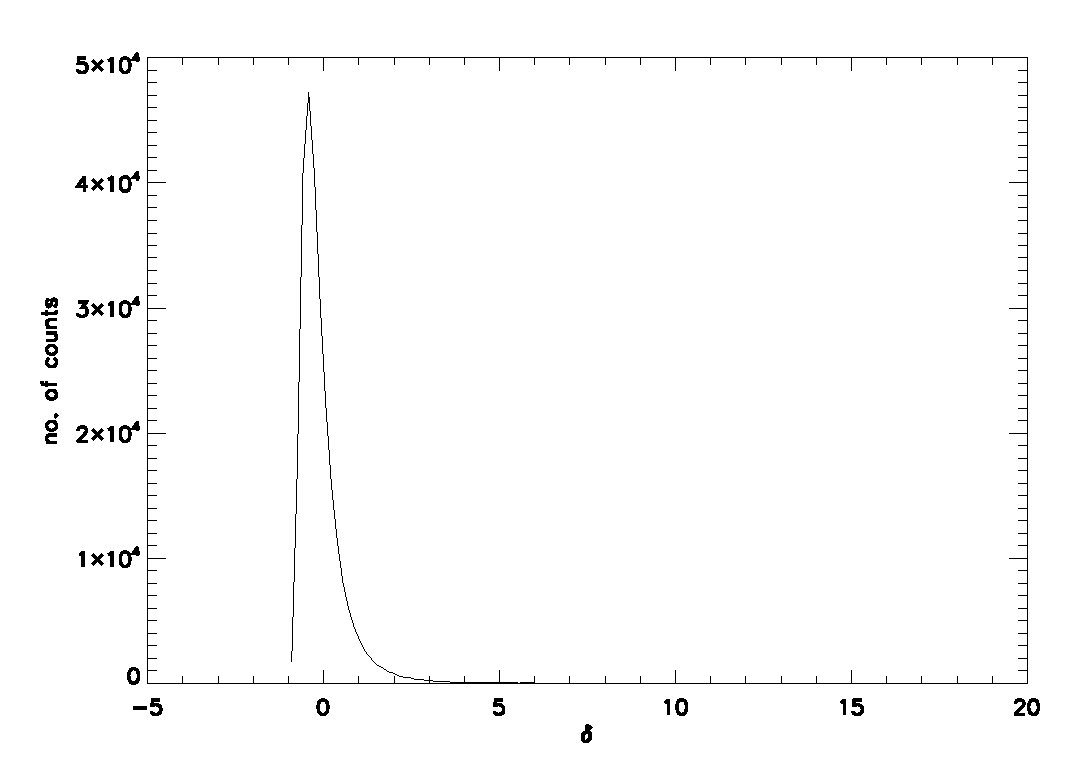
\includegraphics[width=0.49\columnwidth]{./full/gadget/hist_delta_003}
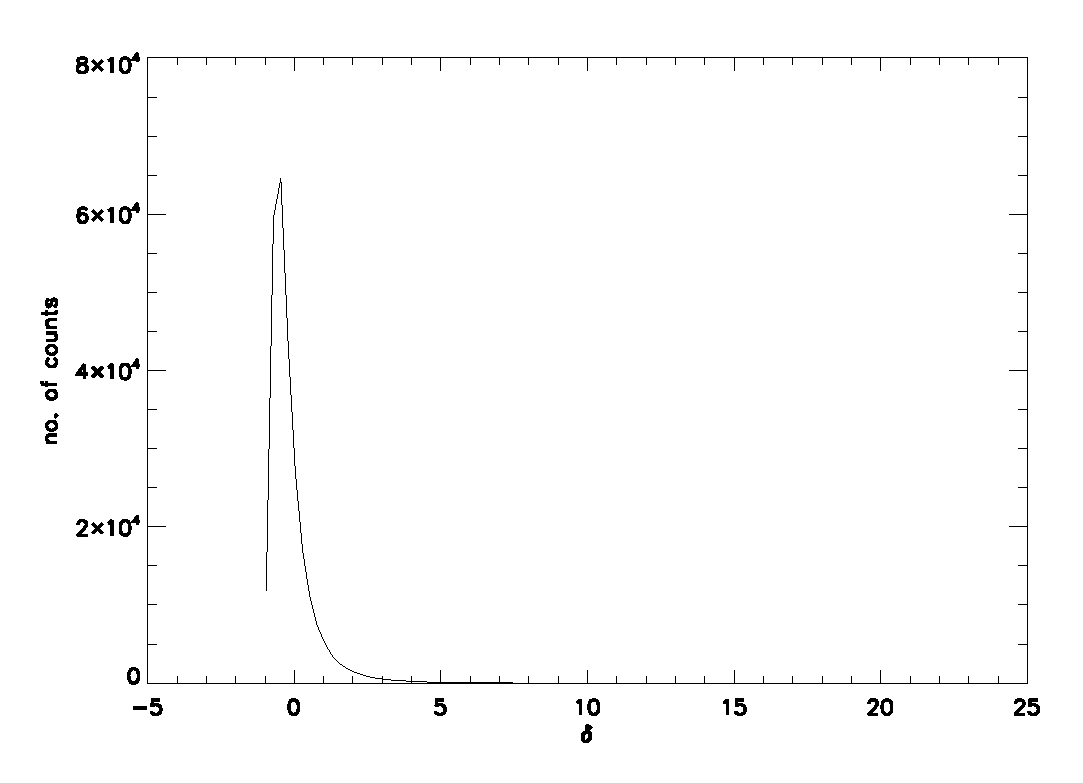
\includegraphics[width=0.49\columnwidth]{./full/gadget/hist_delta_004}

   \end{center}
\caption{These plots show histograms of over-density as generated from the Gadget outputs. The outputs are for $z = 32, 3, 2, 1, 0.5, 0.05.$}
\label{fig.gadhistdc}
\end{figure}

% check velocities are maxwellian?
The evolution of density and over-density from the wave-mechanics code is similar to that of Gadget but not the same. The initial conditions are the same, as required. However, in the wave-mechanics outputs (see figure \ref{fig.wmhist}), the gaussian shape of the density field skews over time with the peak leaning towards the higher mass end. It also develops a long tail, to balance the skewing towards the top end, as the under-dense regions evacuate. The highest peak of density (and over-density) never goes as high as it does in the Gadget outputs. However, the lowest trough of density is far lower than that of Gadget: $\rho_{min} \sim 10^6$ for wave-mechanics while Gadget only goes as low as $\rho_{min} \sim 10^{9.5}$. The under-dense regions are evacuated faster in wave-mechanics, hence the over-density histogram (figure \ref{fig.wmhistdc}) approaches a log-normal shape more rapidly than it does for Gadget. This was not expected but seems to be an inevitable result of wave-mechanics. All resolutions and choice of $\nu$ tested seem to produce similar behaviour, the results shown in figure \ref{fig.wmhistdc} are typical plots.

A further unexpected outcome of wave-mechanics is the rapid variability in the height of density ($\rho$) from gridpoint to gridpoint (see figure \ref{fig.wmrho}). Naturally, the Gadget outputs can be expected to be smoother as they density field is not continuous but rather is calculated from the discrete distribution of particles. The wave-mechanics code gives more lows and more highs (by number count) than Gadget, while the lowest trough and highest peak are lower than that of Gadget. Again, this appears to be true regardless of resolution.

The plots in figure \ref{fig.wmrho} have a resolution of $64^3$ with $\nu = 10^{-7}$ and $|\delta|_{\rm initial} \sim 0.03$, otherwise all initial conditions are the same as for the Gadget simulation. In figure \ref{fig.dc_problem}, we noted there was a problem with the maximum value of $\delta$ being too large. There, $\delta_{max} = 6$ after 100 timesteps when $|\delta|_{\rm initial} \sim 0.3$. In the latest run where $|\delta|_{\rm initial} \sim 0.03$, the $\delta_{max}$ from this simulation after 100 timesteps run was $\delta_{max} = 0.7$. This is of a more acceptable magnitude.

In addition to the histograms (\ref{fig.wmhist}, \ref{fig.wmhistdc}) and the surface plots of density (\ref{fig.wmrho}), I provide a contour plot of over-density (figure \ref{fig.delta_contour}) which has levels at $\delta =  -1, 0, 1, 2, 5$. From the surface plots (\ref{fig.wmrho}) it is hard, at first, to tell if the structure is random as it appears to rapidly change from timestep to timestep. The data is messier than from Gadget, so the conclusion is not as immediately obvious. The contour plots give the clearest picture of how the structure is fragmentary but not completely random. Implicitly, the data has been smoothed to hide the finest structure.

A possible source of such messiness is due to the fact that the whole simulation uses a single coherent wavefunction. As shown in the results of section \ref{per_bou}, a single wavefunction can lead to interference effects. Although we hope to limit this effect by using a small $\nu$ we may not have completely suppressed these effects. That is despite the fact gravity also acts to suppress such interference effects.

In contrast to the Gadget density, the plots of wave-mechanics show more structure. For comparison we can look at the contour plots generated for Gadget (figure \ref{fig.gadget_contour}). These latter plots are far smoother than that of wave-mechanics. It seems also impossible to tell that the results of wave-mechanics and Gadget come from the same initial conditions. It should be noted that the highest value of $\delta$ for Gadget was $\delta \sim 23$, which is far higher than that of wave-mechanics $\delta \sim 9 \rightarrow 14$ (depending on parameter choice: such as varying $\nu$).


All of the following outputs are shown for timesteps: $0, 200, 1000, 2000, 3000, 3500$, or $a = 0.03125,0.038,0.085,0.23, 0.63, 1.03$. The slices through the data were all taken at the some point on the z-axis: $L/2$.


\begin{figure}[htb]
   \begin{center}
     %\leavevmode

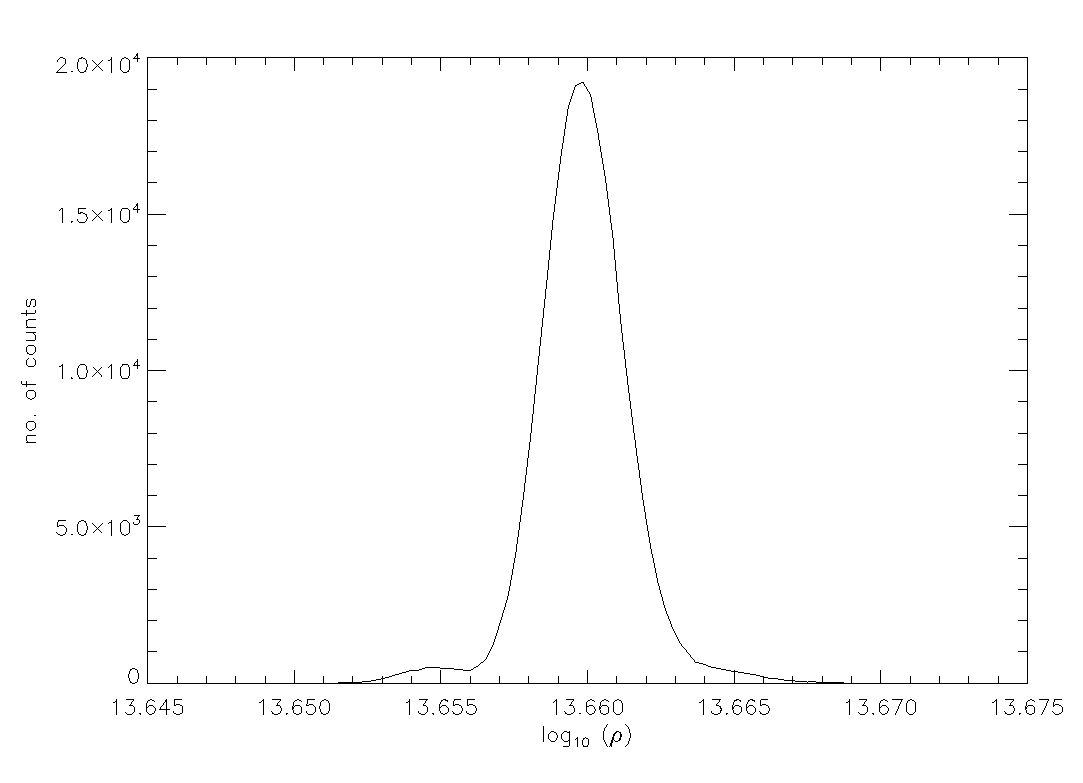
\includegraphics[width=0.49\columnwidth]{./full/wm64/hist/r00000_hist}
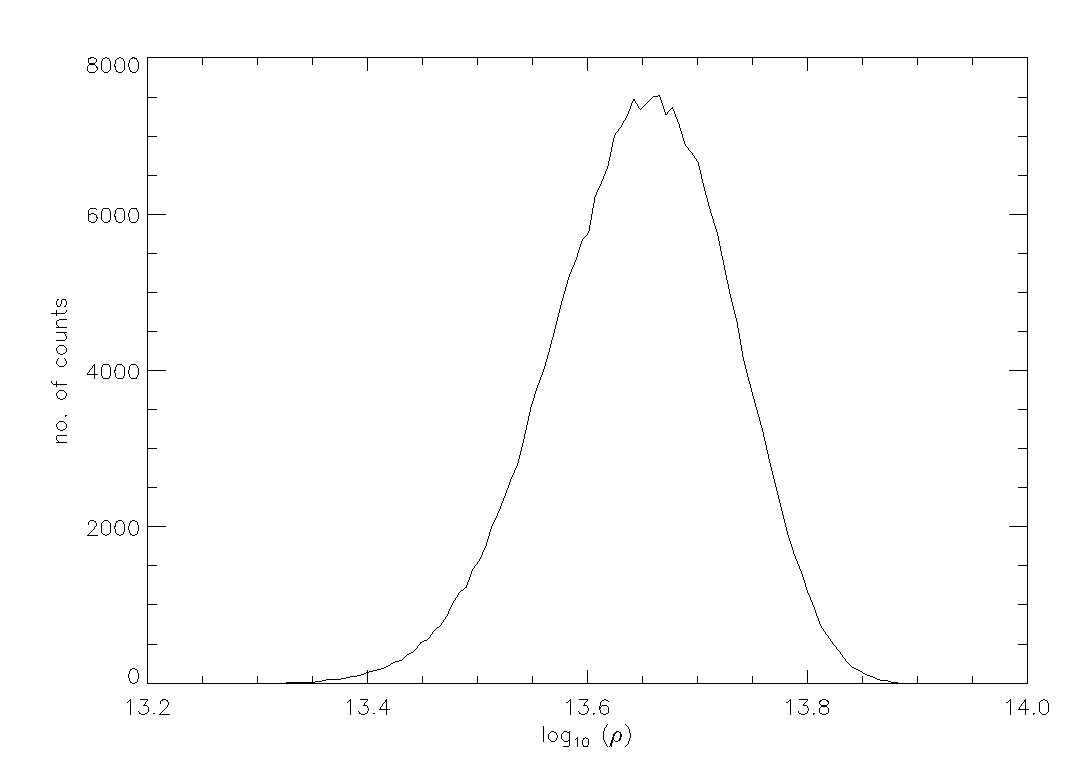
\includegraphics[width=0.49\columnwidth]{./full/wm64/hist/r00200_hist}
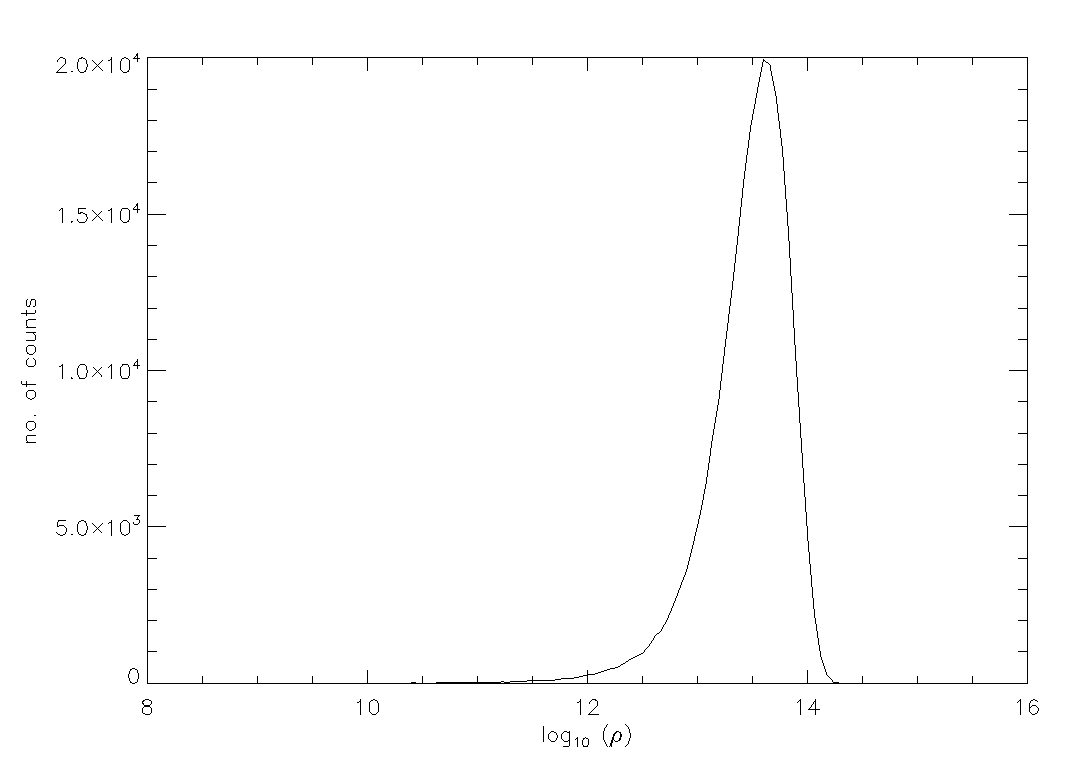
\includegraphics[width=0.49\columnwidth]{./full/wm64/hist/r01000_hist}
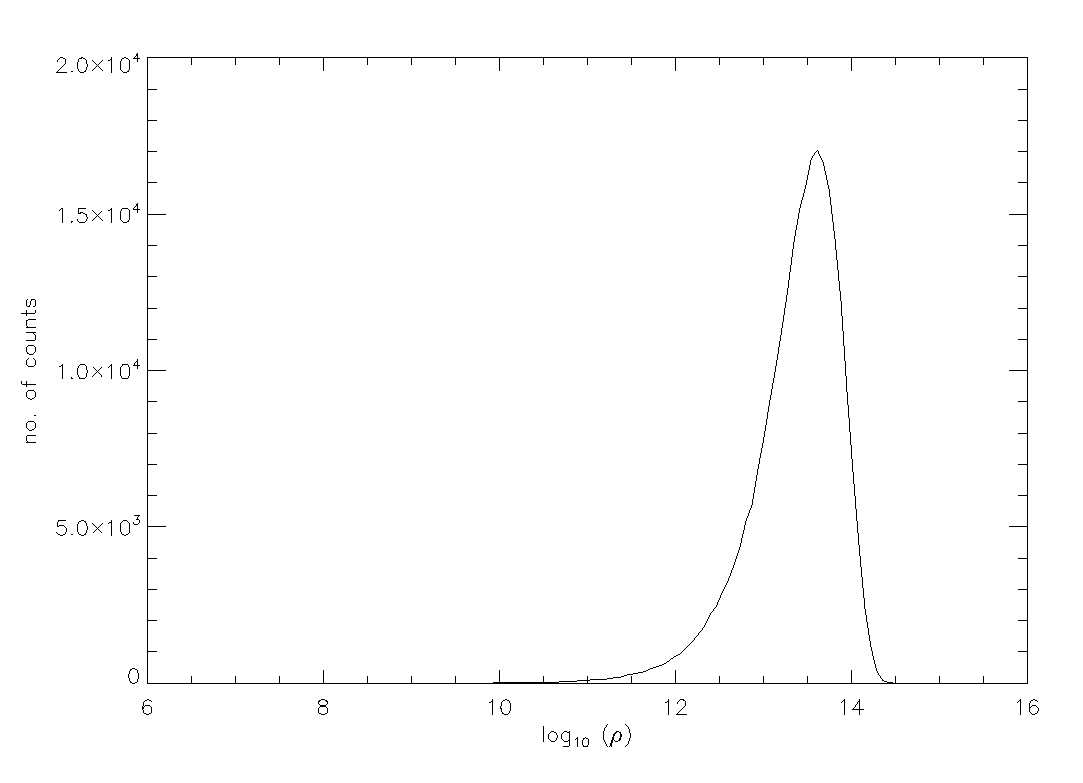
\includegraphics[width=0.49\columnwidth]{./full/wm64/hist/r02000_hist}
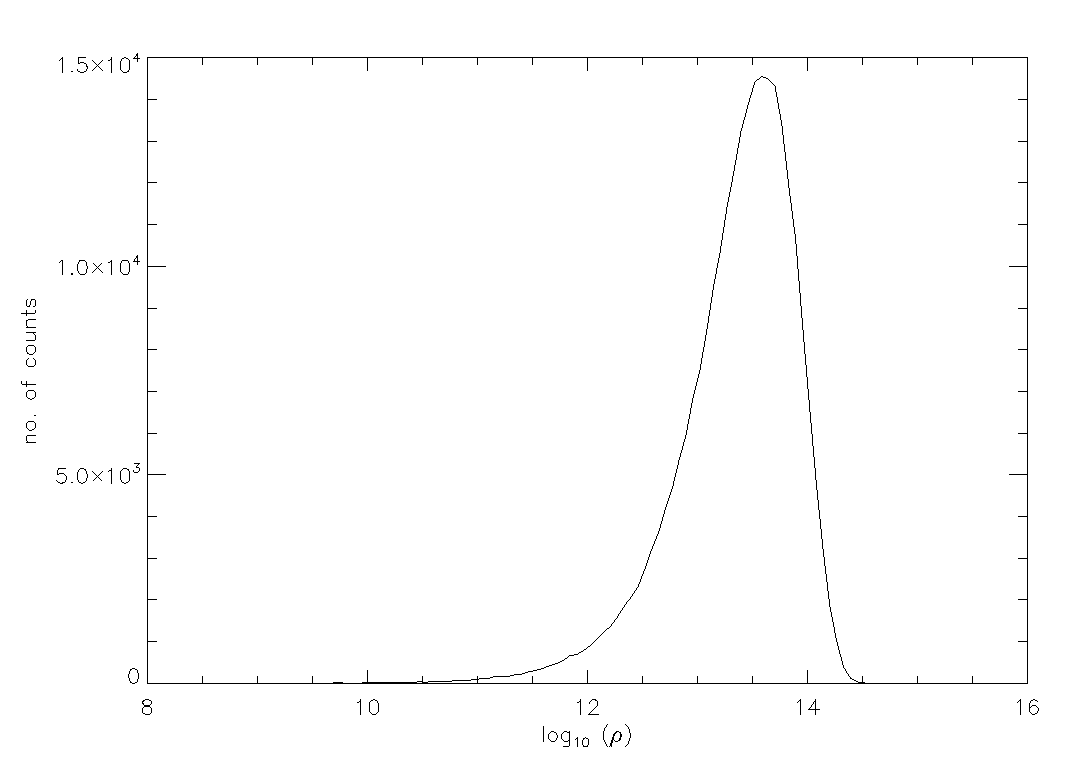
\includegraphics[width=0.49\columnwidth]{./full/wm64/hist/r03000_hist}
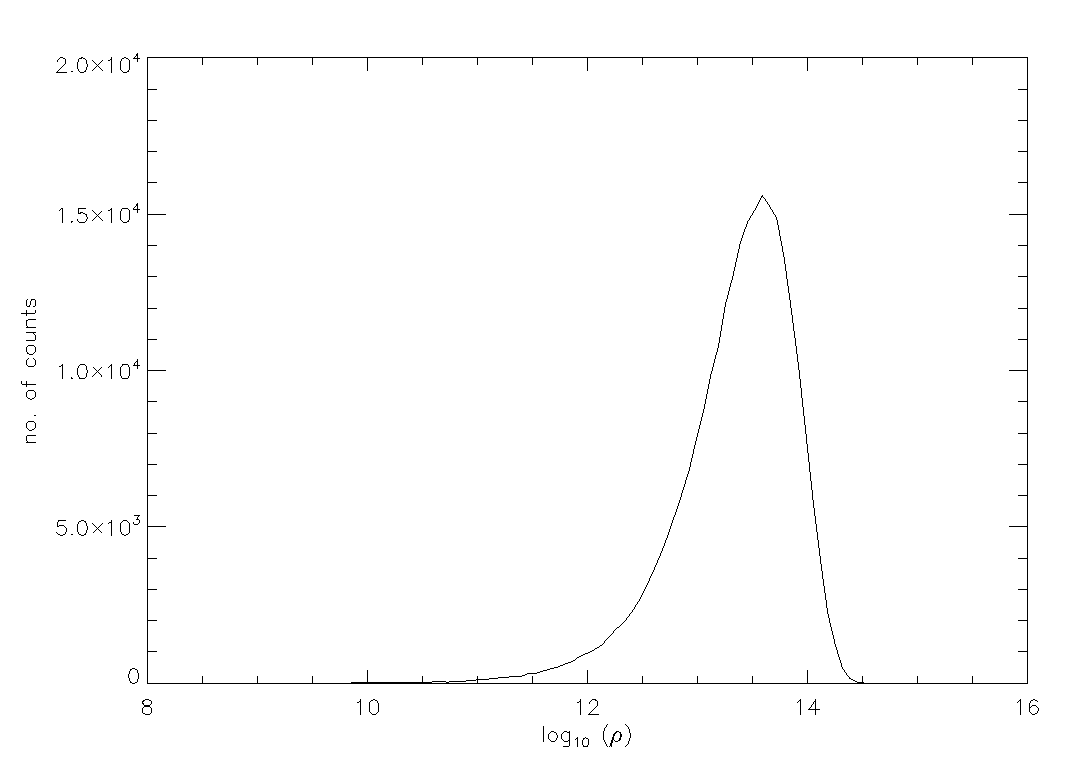
\includegraphics[width=0.49\columnwidth]{./full/wm64/hist/r03500_hist}

   \end{center}
\caption{These plots show histograms of density ($\rho$) as generated from the wave-mechanics code. They have a distinctly gaussian shape but widen and skew over time. The outputs at $t = 0, 200, 1000,$ $2000, 3000, 3500$ ($a = 0.03125,0.038,$ $0.085,0.23, 0.63, 1.03$).}
\label{fig.wmhist}
\end{figure}

\begin{figure}[htb]
   \begin{center}
     %\leavevmode

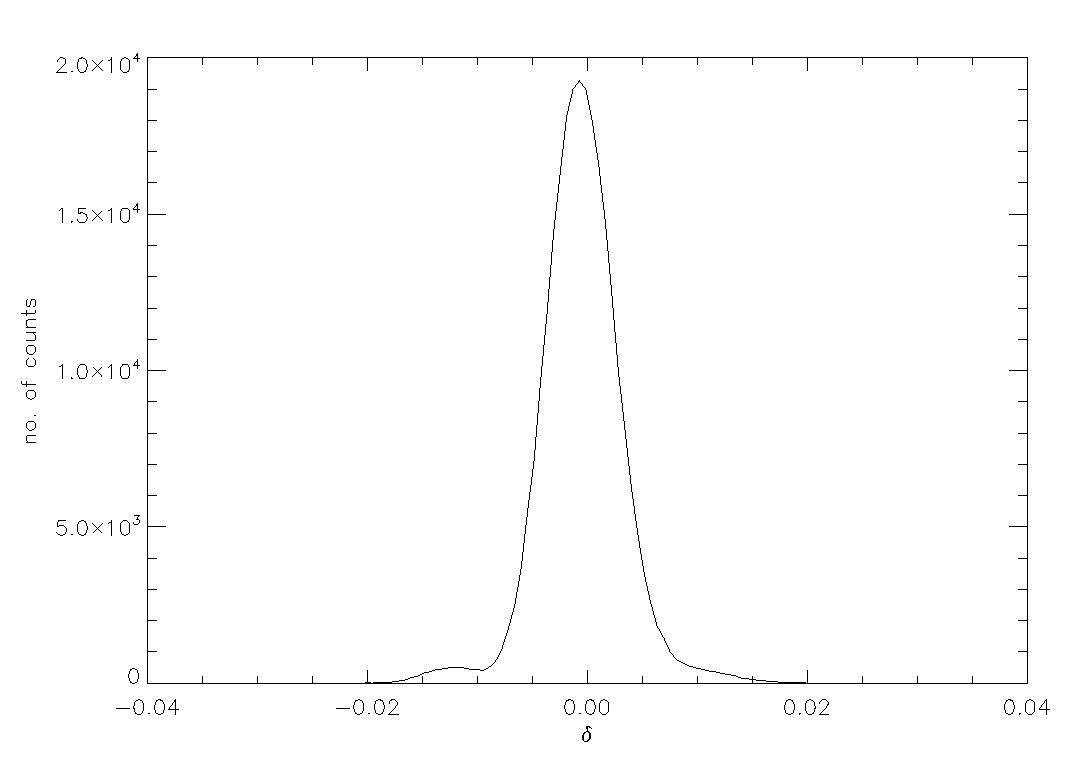
\includegraphics[width=0.49\columnwidth]{./full/wm64/hist/r00000_hist_dc}
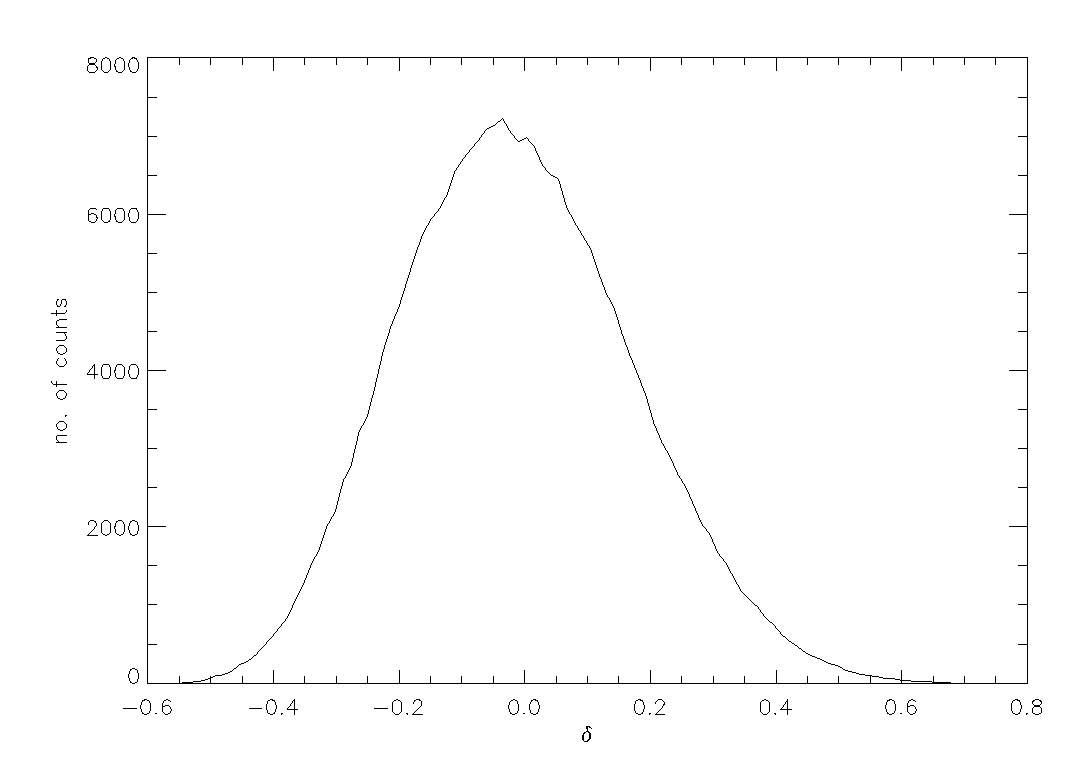
\includegraphics[width=0.49\columnwidth]{./full/wm64/hist/r00200_hist_dc}
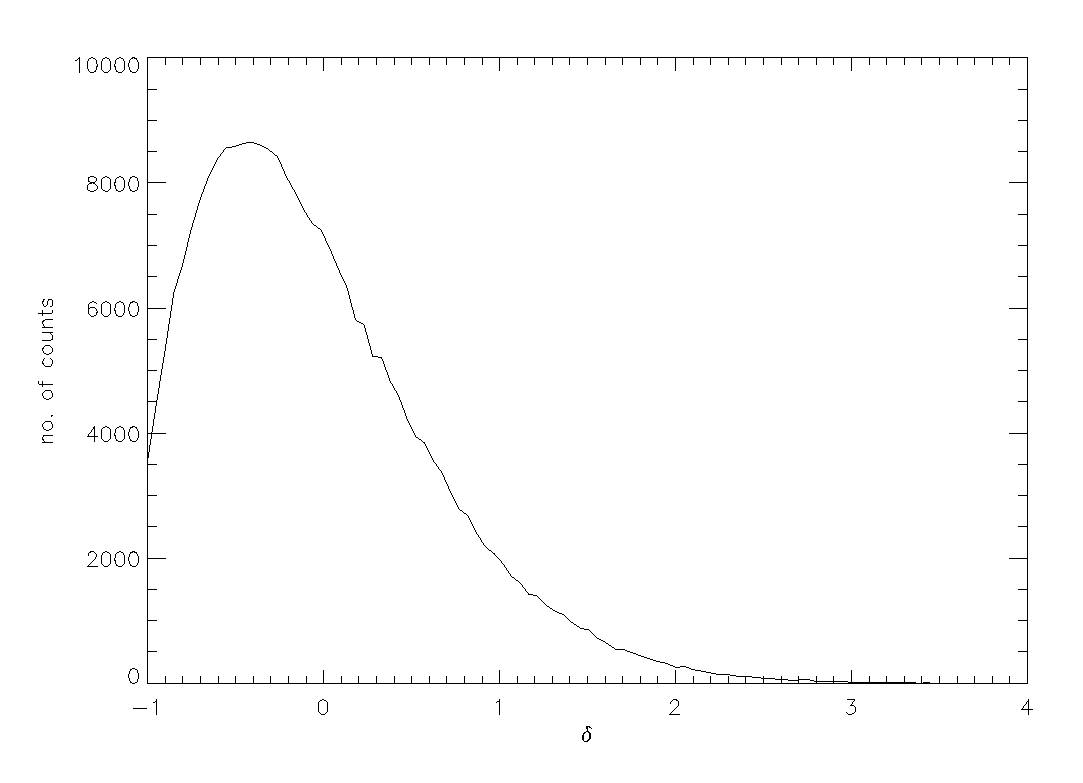
\includegraphics[width=0.49\columnwidth]{./full/wm64/hist/r01000_hist_dc}
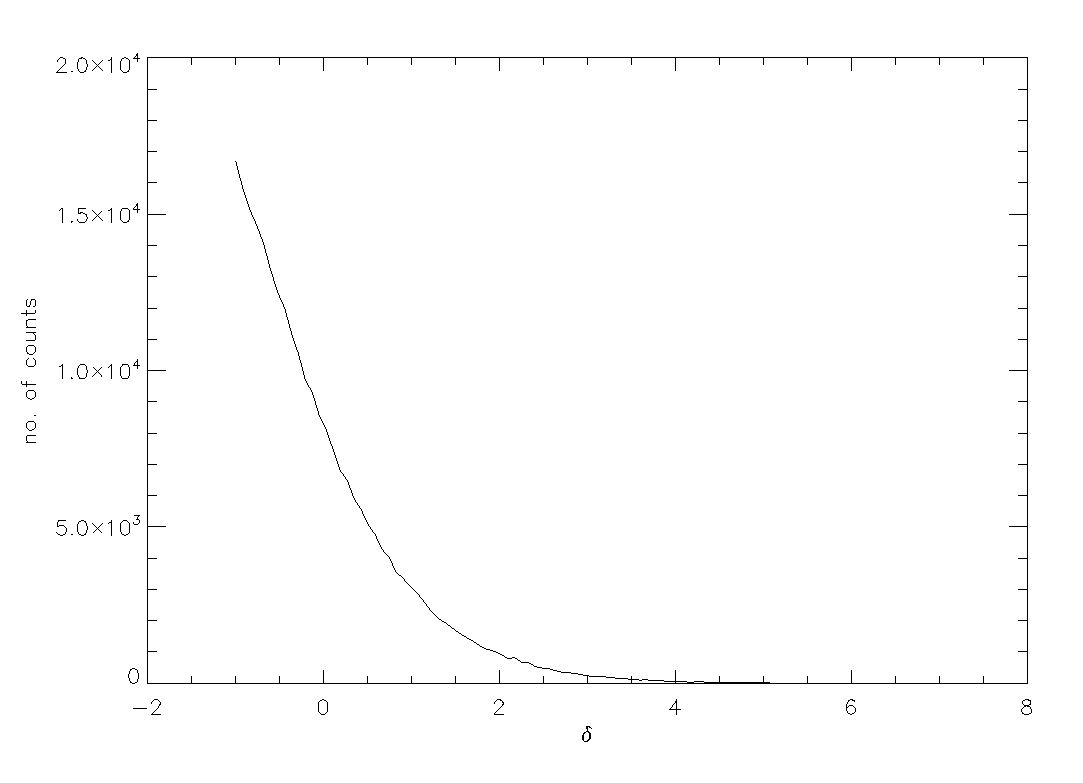
\includegraphics[width=0.49\columnwidth]{./full/wm64/hist/r02000_hist_dc}
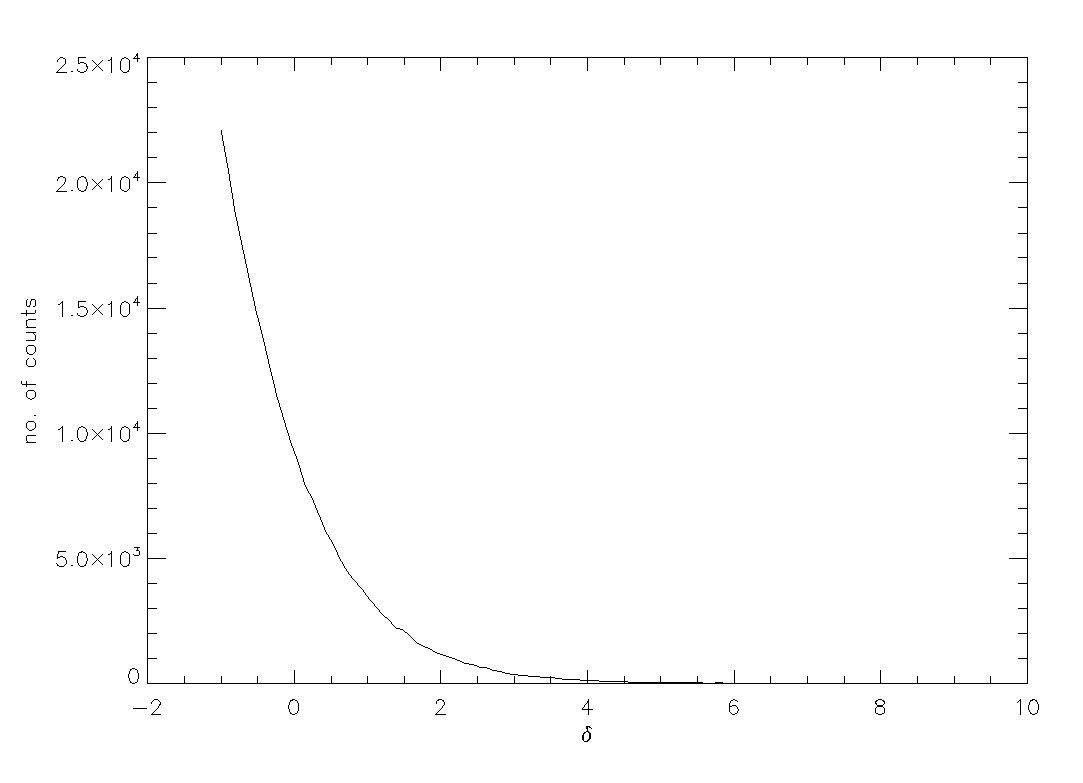
\includegraphics[width=0.49\columnwidth]{./full/wm64/hist/r03000_hist_dc}
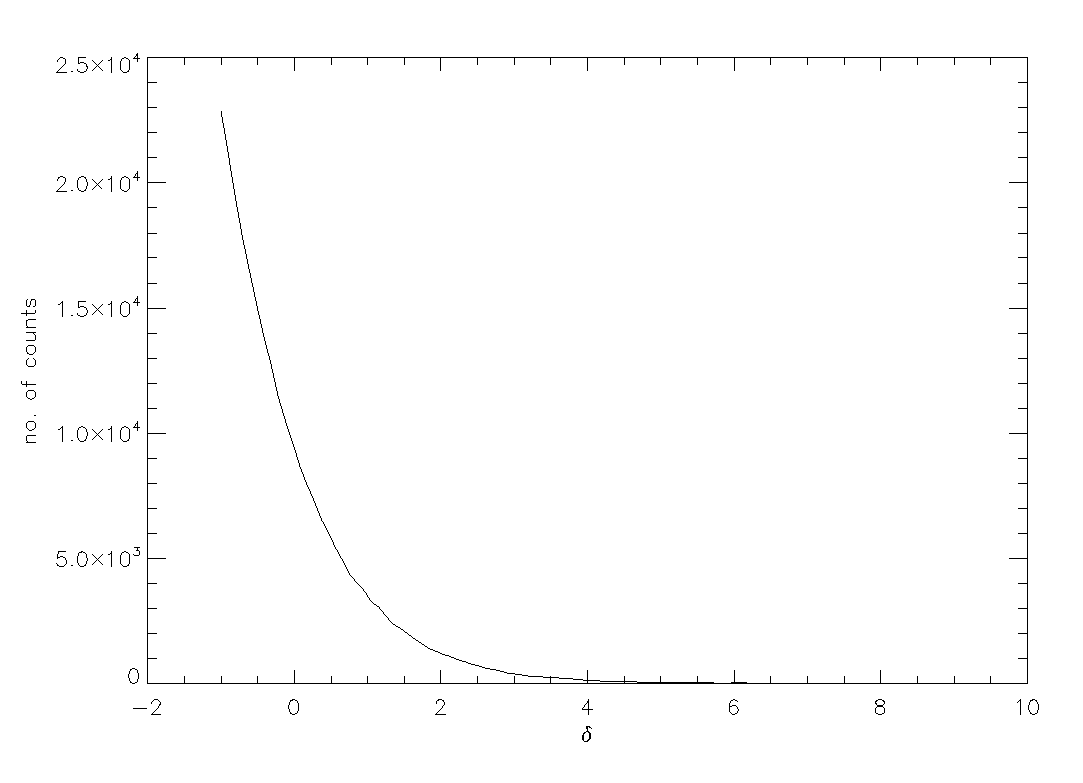
\includegraphics[width=0.49\columnwidth]{./full/wm64/hist/r03500_hist_dc}

   \end{center}
\caption{These plots show histograms of density contrast ($\delta$) as generated from the wave-mechanics code. Outputs at $t = 0, 200, 1000, 2000, 3000, 3500$.}
\label{fig.wmhistdc}
\end{figure}

\begin{figure}[htb]
   \begin{center}
     %\leavevmode

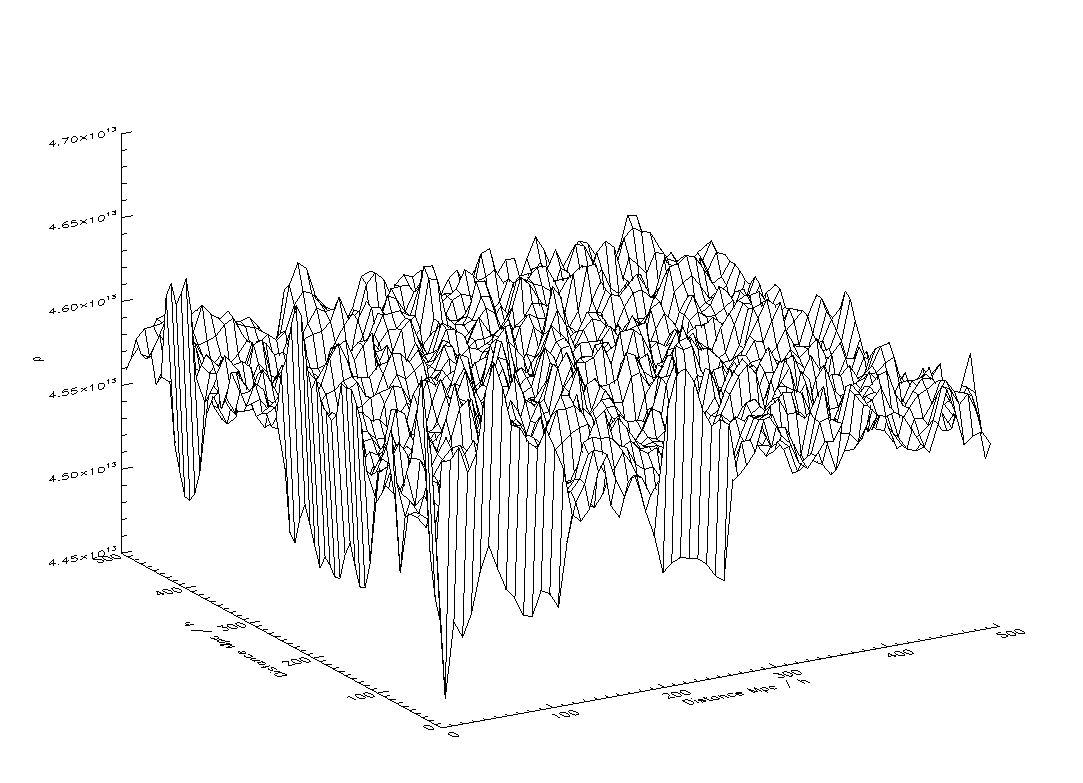
\includegraphics[width=0.49\columnwidth]{./full/wm64/rho/r00000}
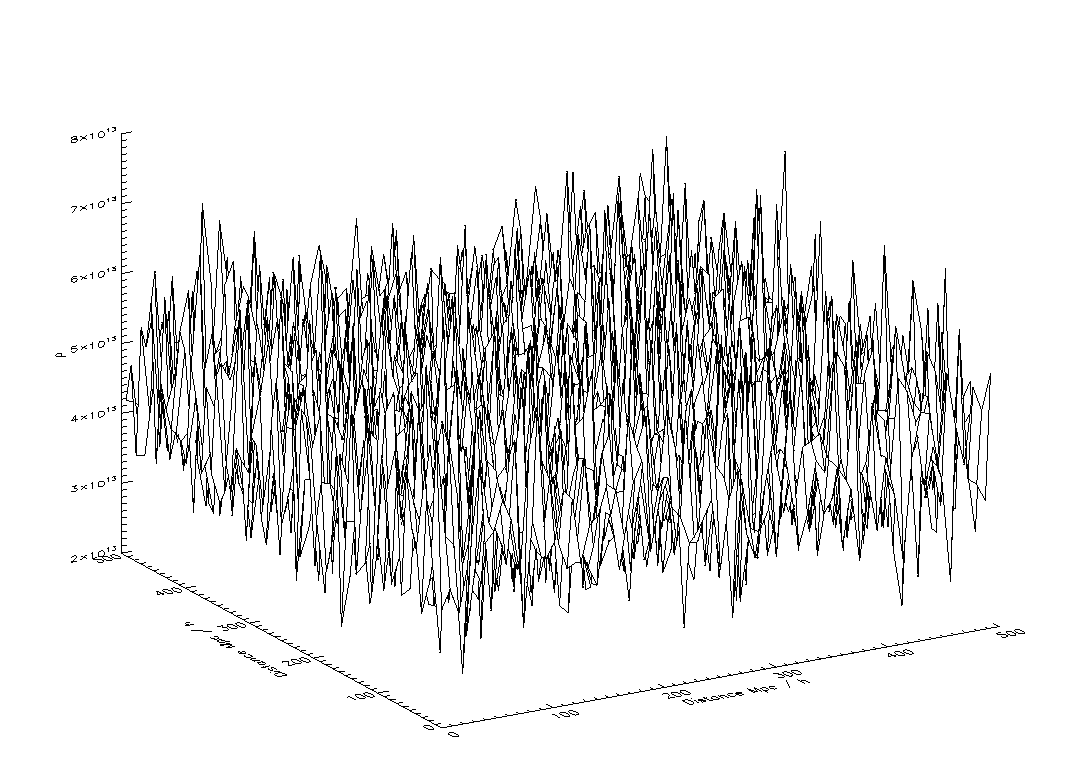
\includegraphics[width=0.49\columnwidth]{./full/wm64/rho/r00200}
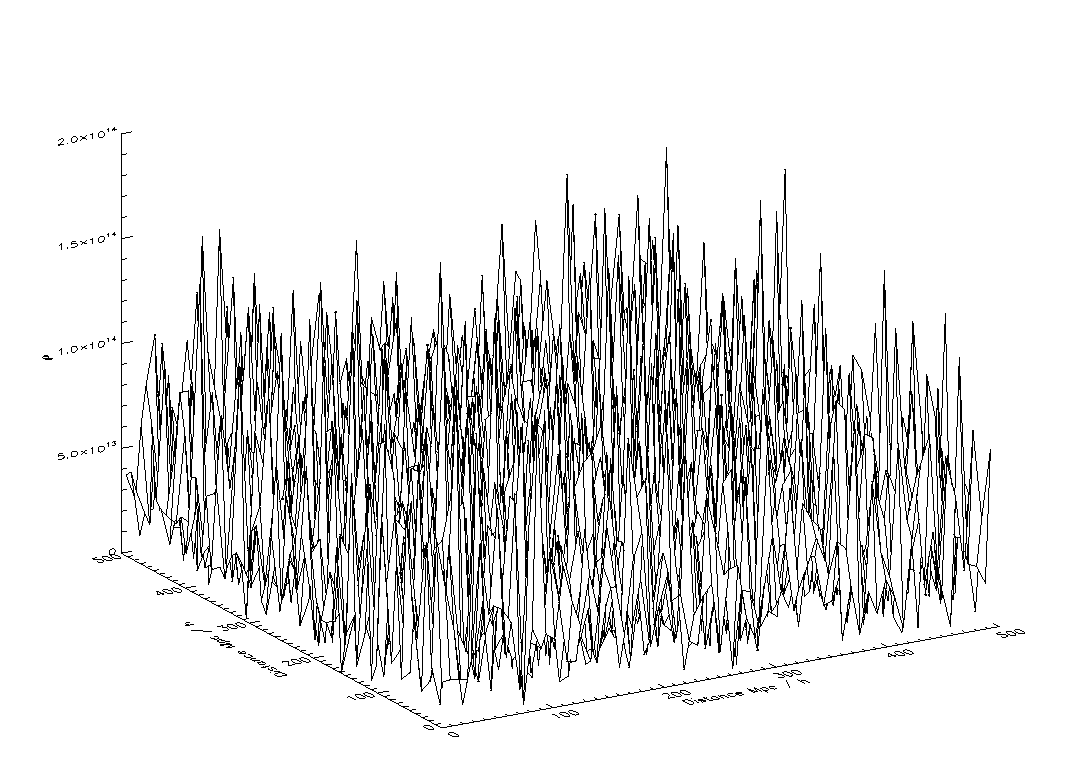
\includegraphics[width=0.49\columnwidth]{./full/wm64/rho/r01000}
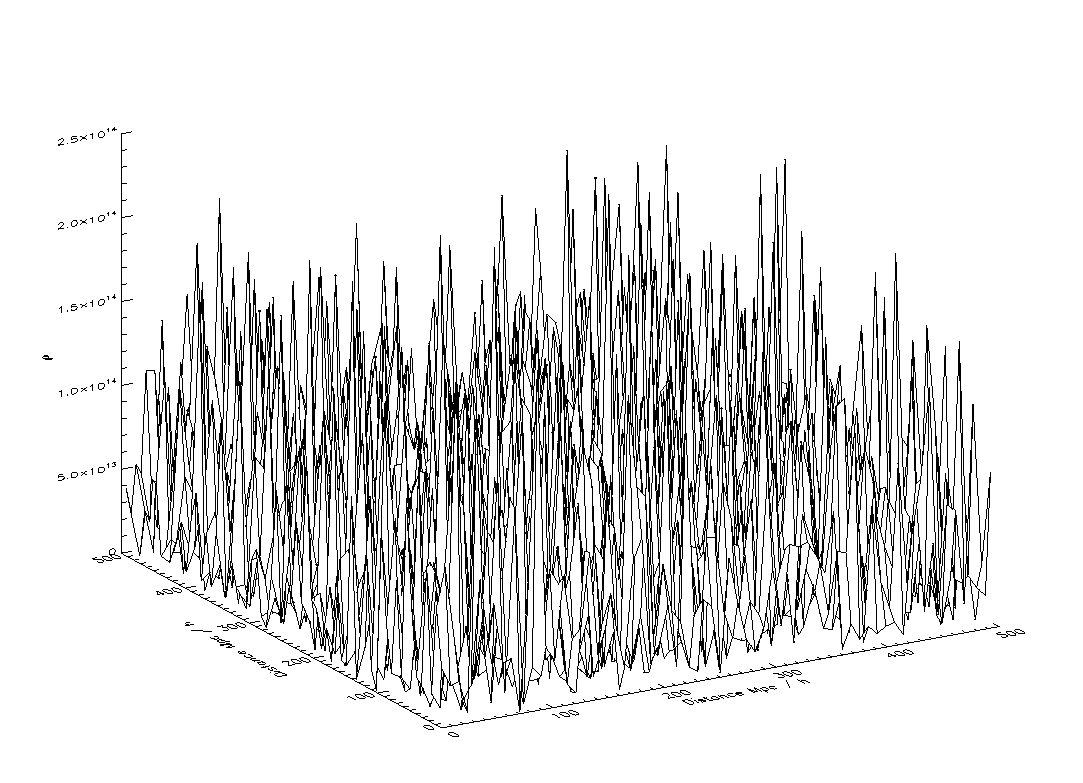
\includegraphics[width=0.49\columnwidth]{./full/wm64/rho/r02000}
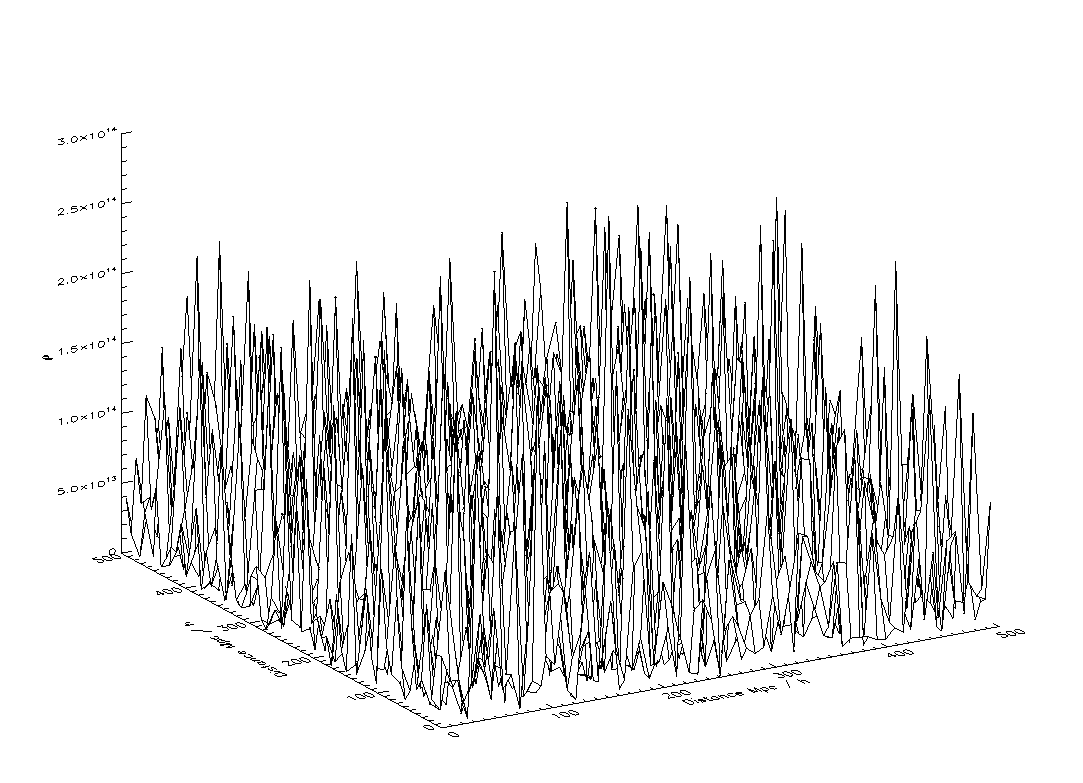
\includegraphics[width=0.49\columnwidth]{./full/wm64/rho/r03000}
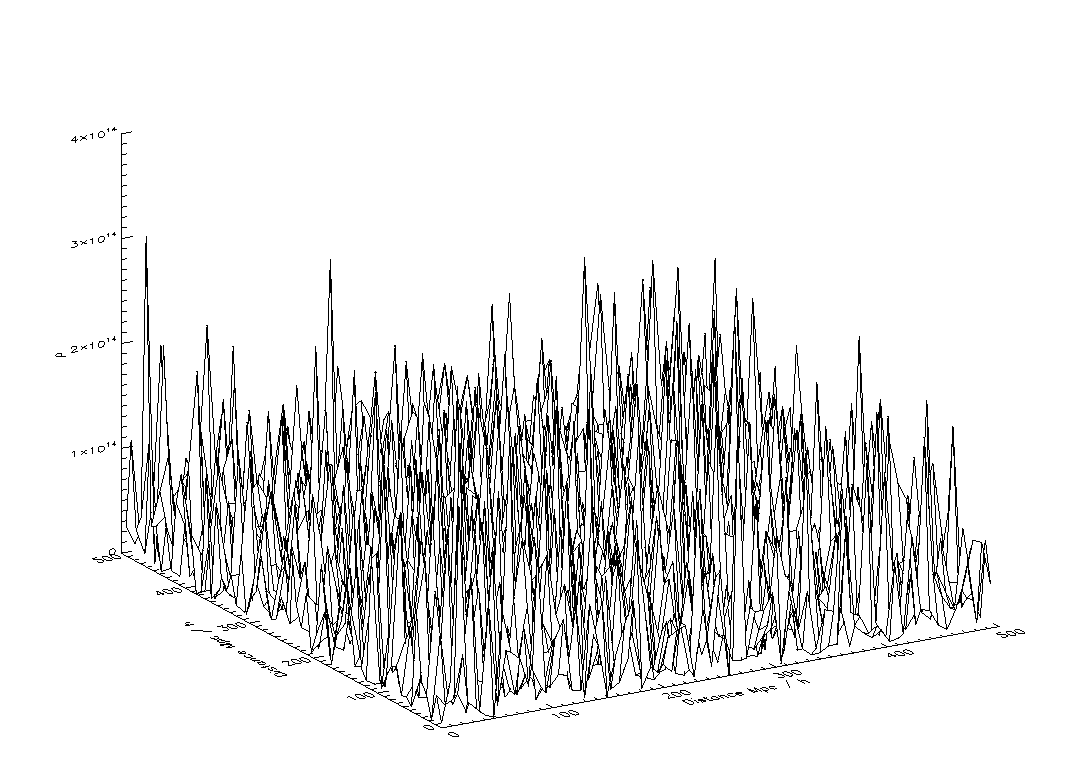
\includegraphics[width=0.49\columnwidth]{./full/wm64/rho/r03500}

   \end{center}
\caption{These plots show a surface plot of density $\rho$ from the wave-mechanics code. The outputs are for timesteps $0, 200, 1000, 2000, 3000, 3500$.}
\label{fig.wmrho}
\end{figure}

\begin{figure}[htb]
   \begin{center}
     %\leavevmode

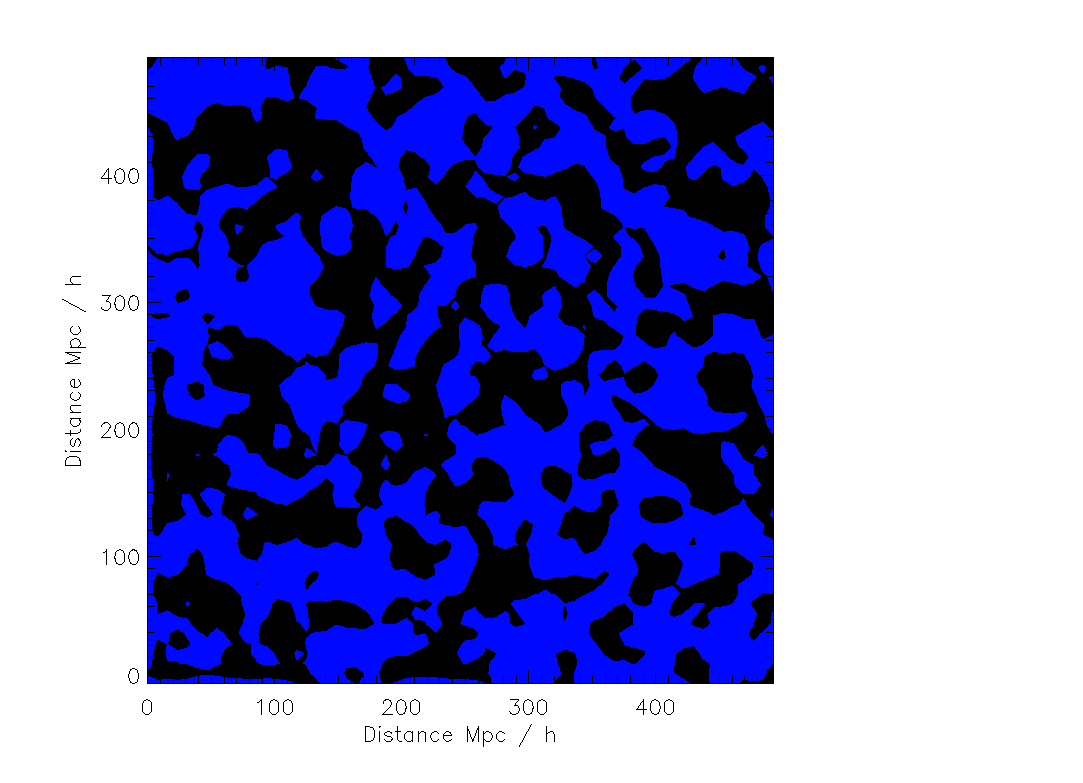
\includegraphics[width=0.49\columnwidth]{./full/wm64/rho_con/r00000_del_contour}
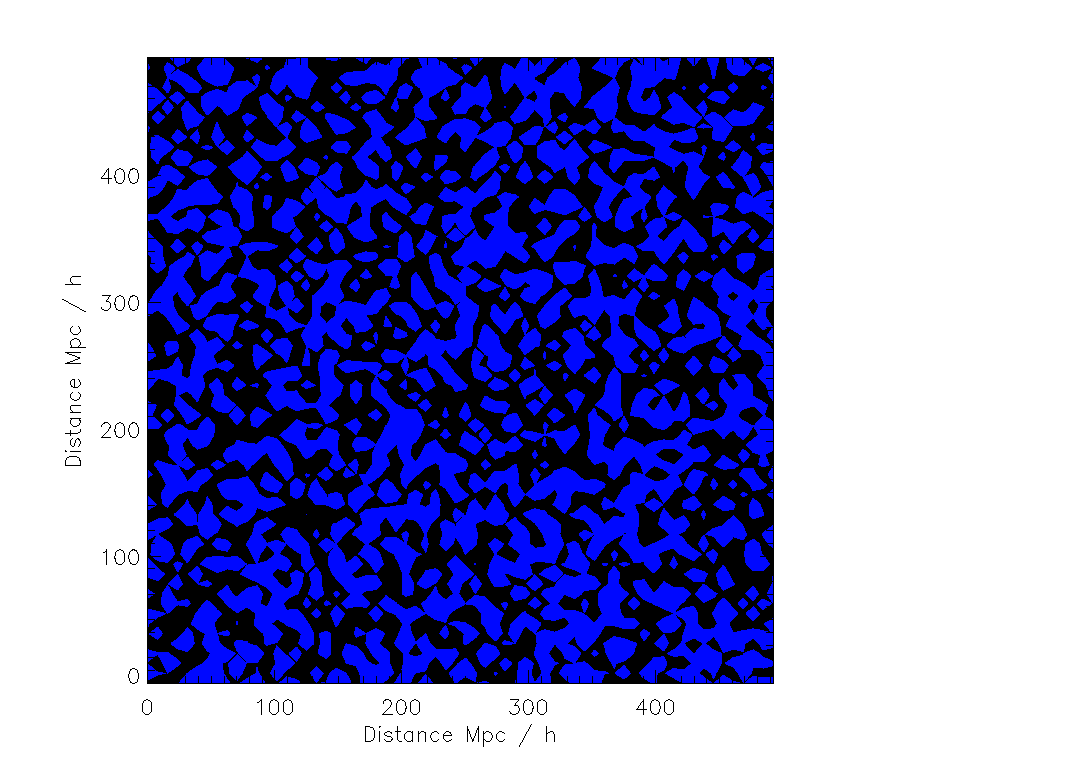
\includegraphics[width=0.49\columnwidth]{./full/wm64/rho_con/r00200_del_contour}
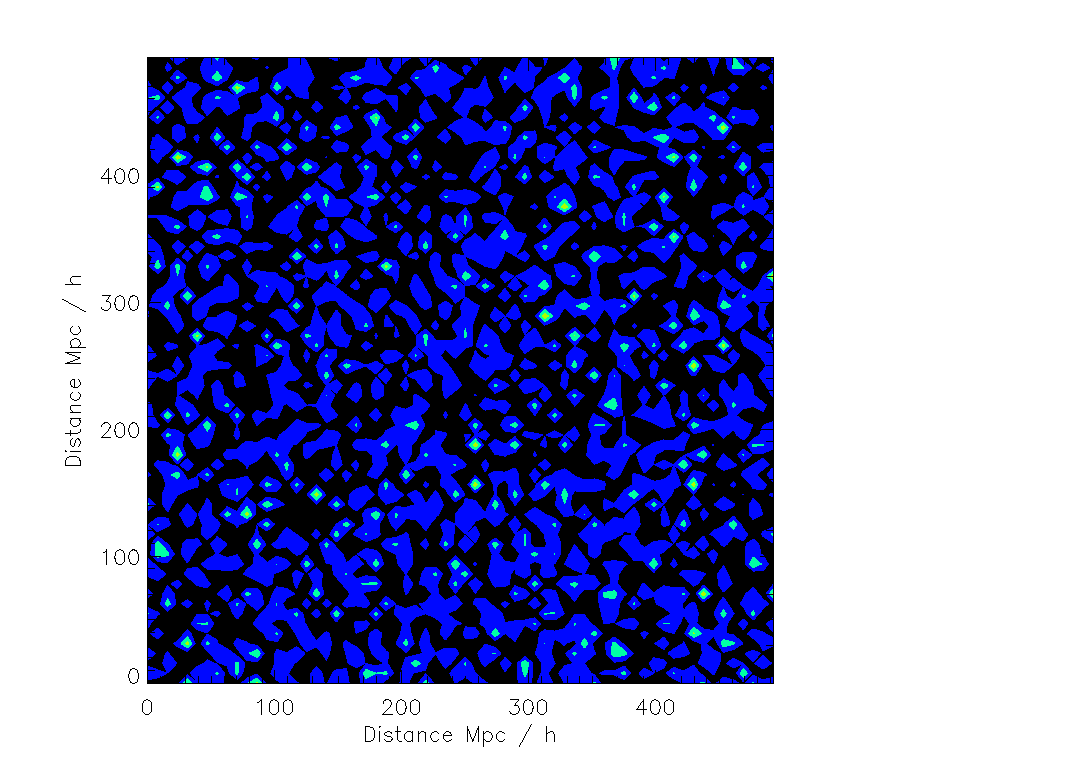
\includegraphics[width=0.49\columnwidth]{./full/wm64/rho_con/r01000_del_contour}
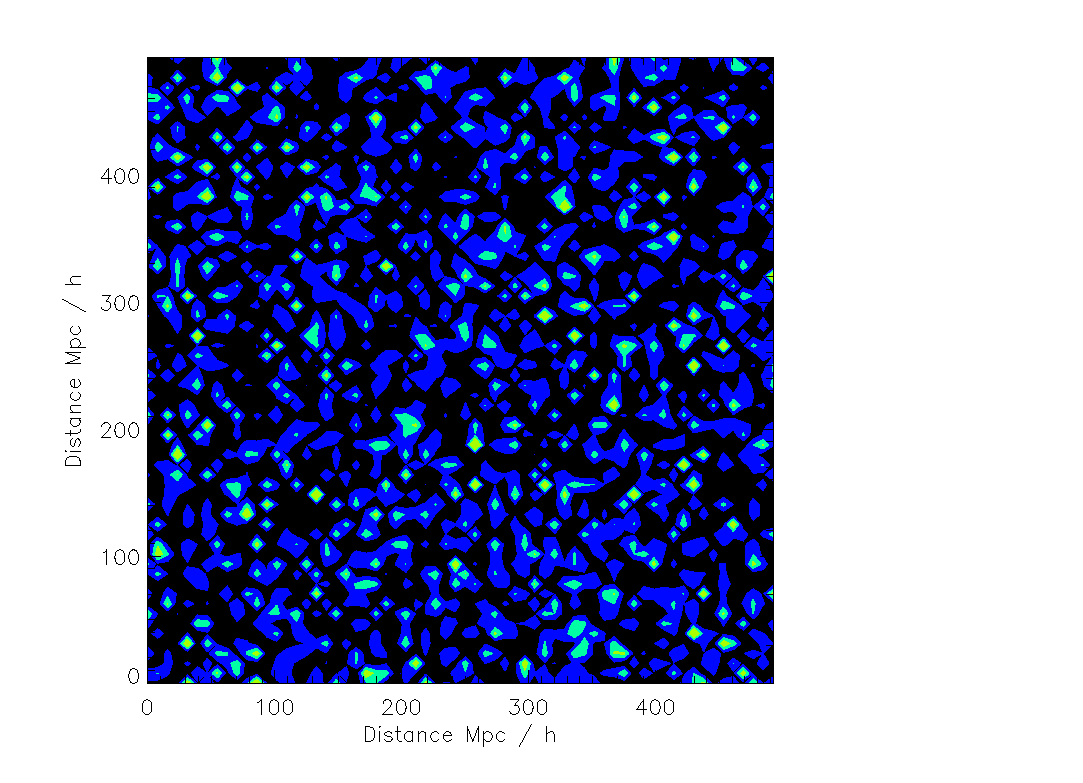
\includegraphics[width=0.49\columnwidth]{./full/wm64/rho_con/r02000_del_contour}
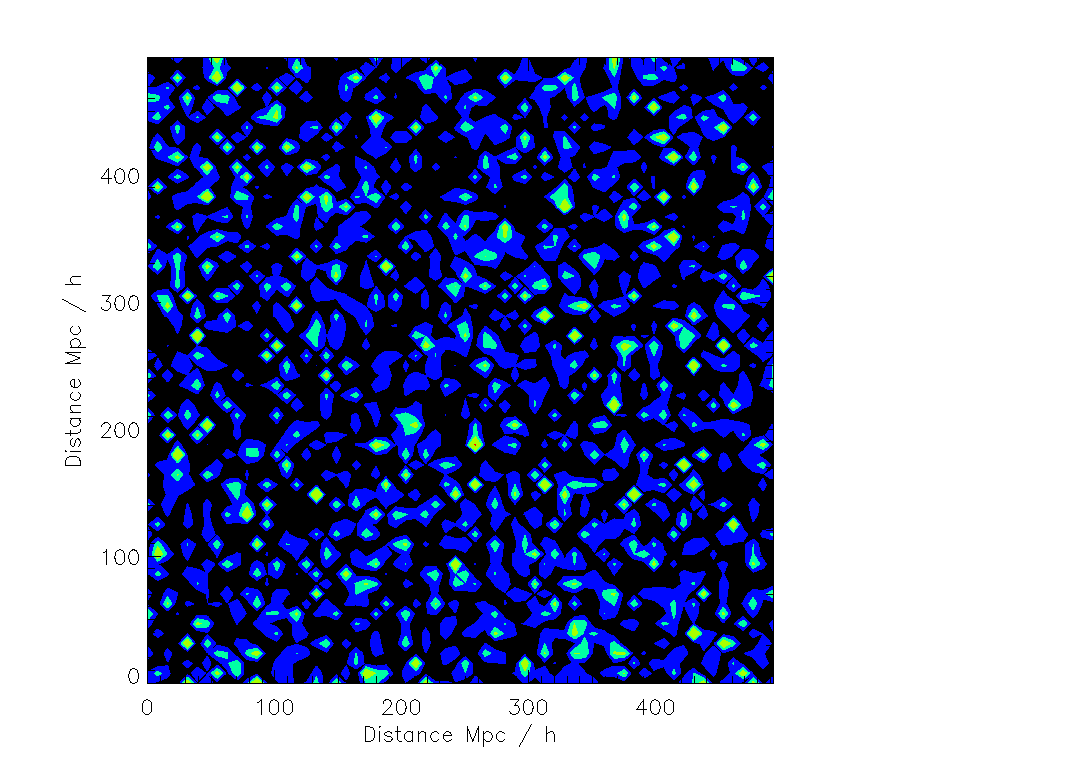
\includegraphics[width=0.49\columnwidth]{./full/wm64/rho_con/r03000_del_contour}
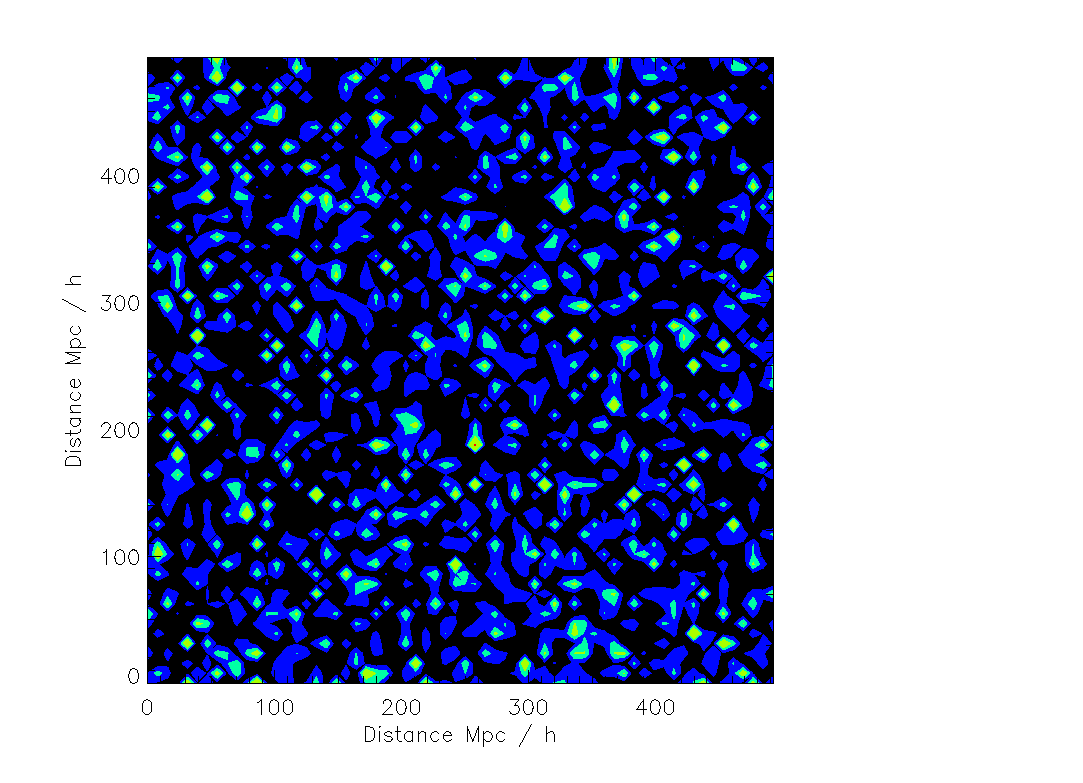
\includegraphics[width=0.49\columnwidth]{./full/wm64/rho_con/r03500_del_contour}

   \end{center}
\caption{These plots show a contour plot of density contrast ($\delta$) from the wave-mechanics simulation. The box length is $L = 500 \; {\rm Mpc / h}$ on each side. The contour levels are $\delta = -1, 0, 1, 2, 5$. The outputs are for timesteps $0, 200, 1000, 2000, 3000, 3500$.}
\label{fig.delta_contour}
\end{figure}

\begin{figure}[htb]
   \begin{center}
     %\leavevmode

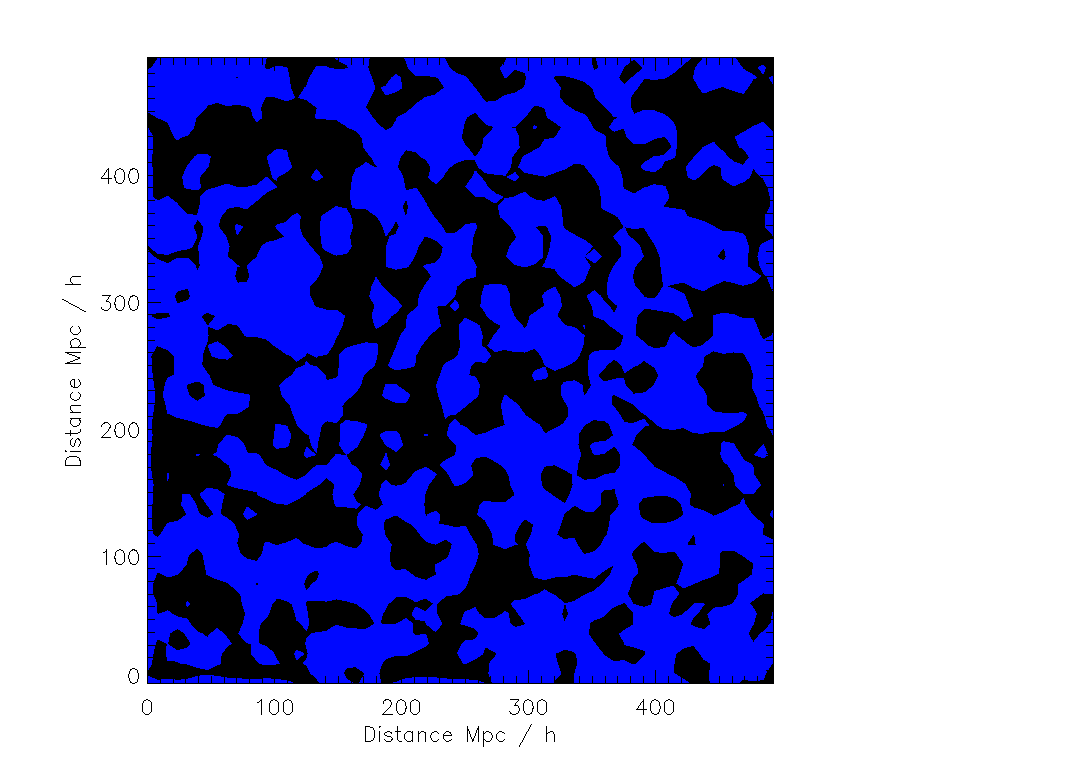
\includegraphics[width=0.49\columnwidth]{./full/gadget/contour/del_contour0000}
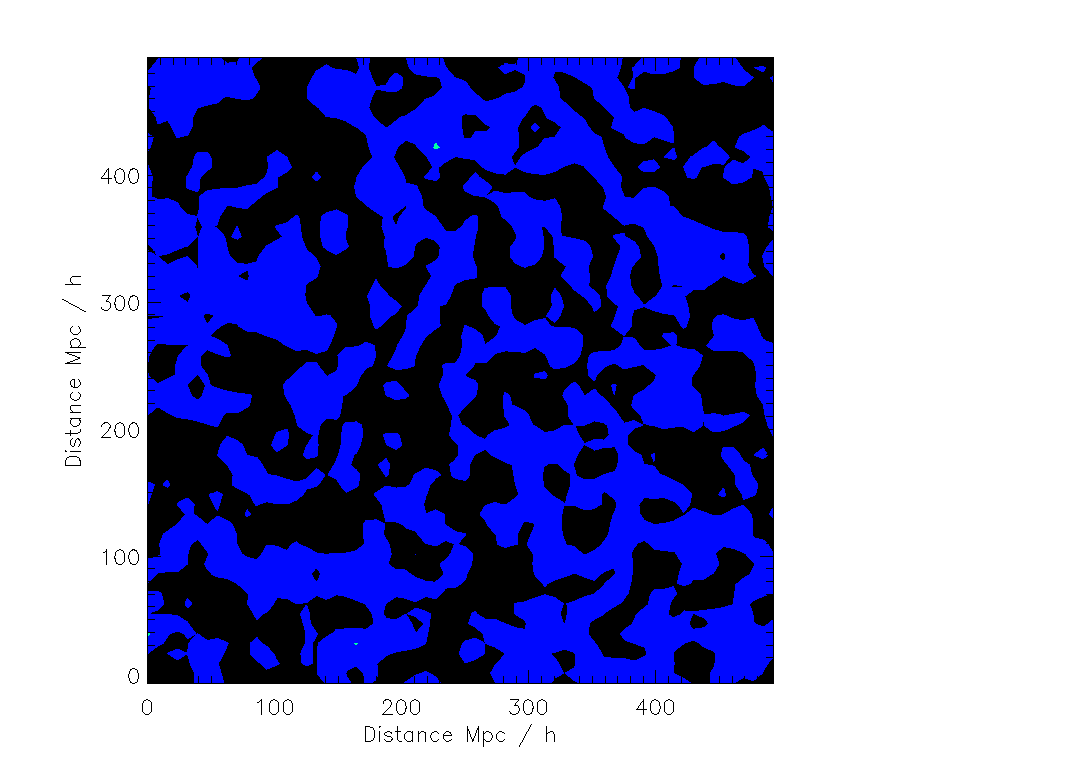
\includegraphics[width=0.49\columnwidth]{./full/gadget/contour/del_contour000}
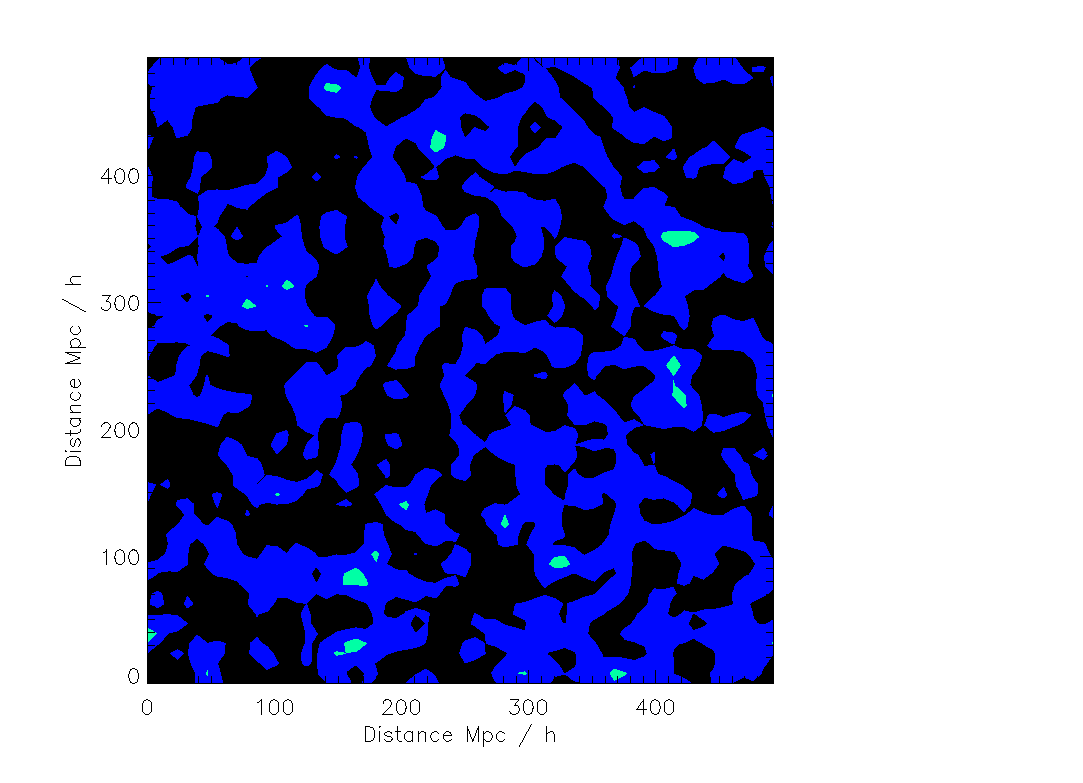
\includegraphics[width=0.49\columnwidth]{./full/gadget/contour/del_contour001}
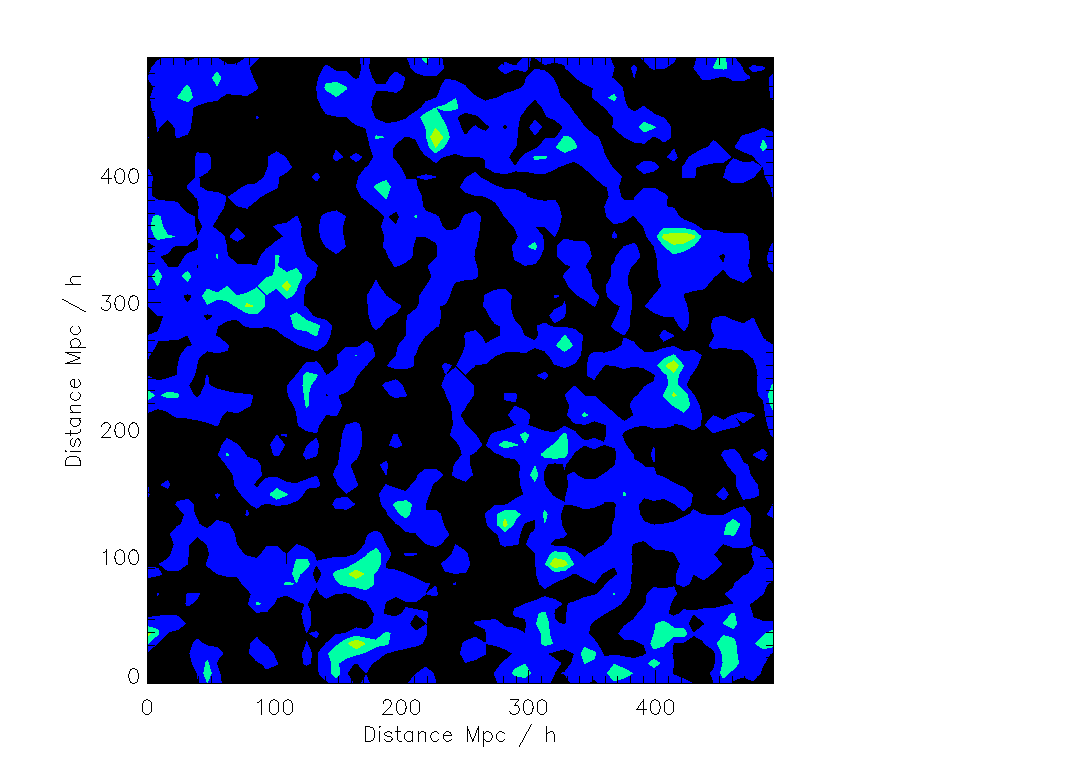
\includegraphics[width=0.49\columnwidth]{./full/gadget/contour/del_contour002}
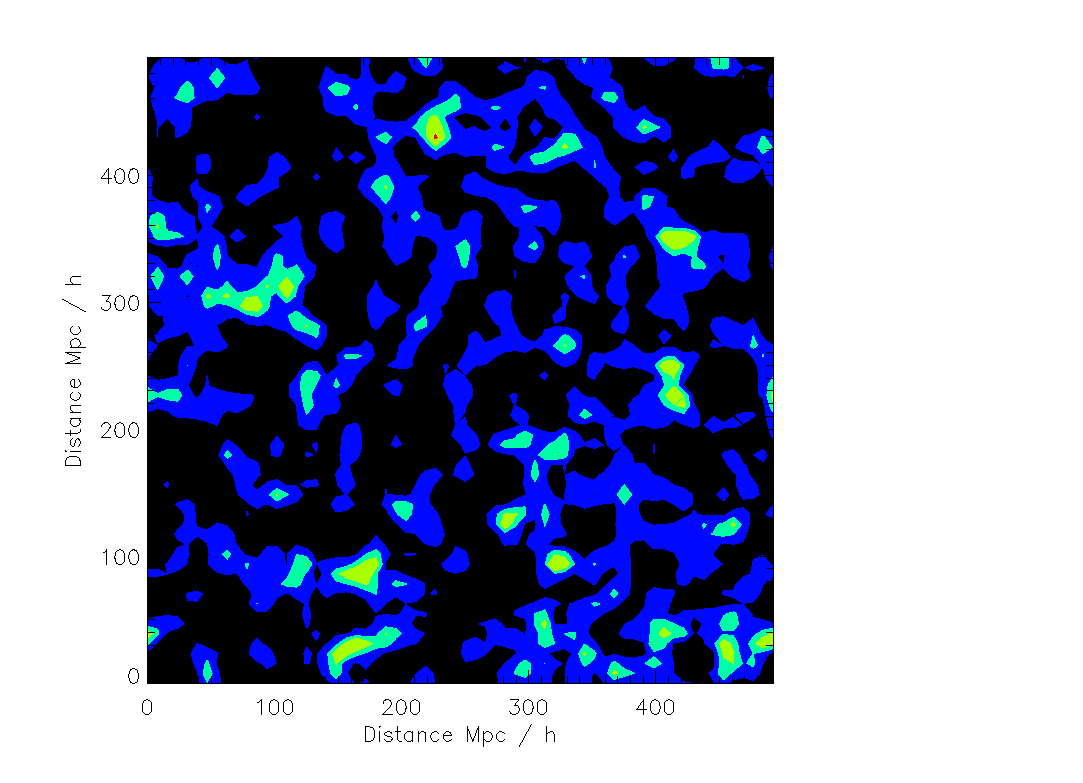
\includegraphics[width=0.49\columnwidth]{./full/gadget/contour/del_contour003}
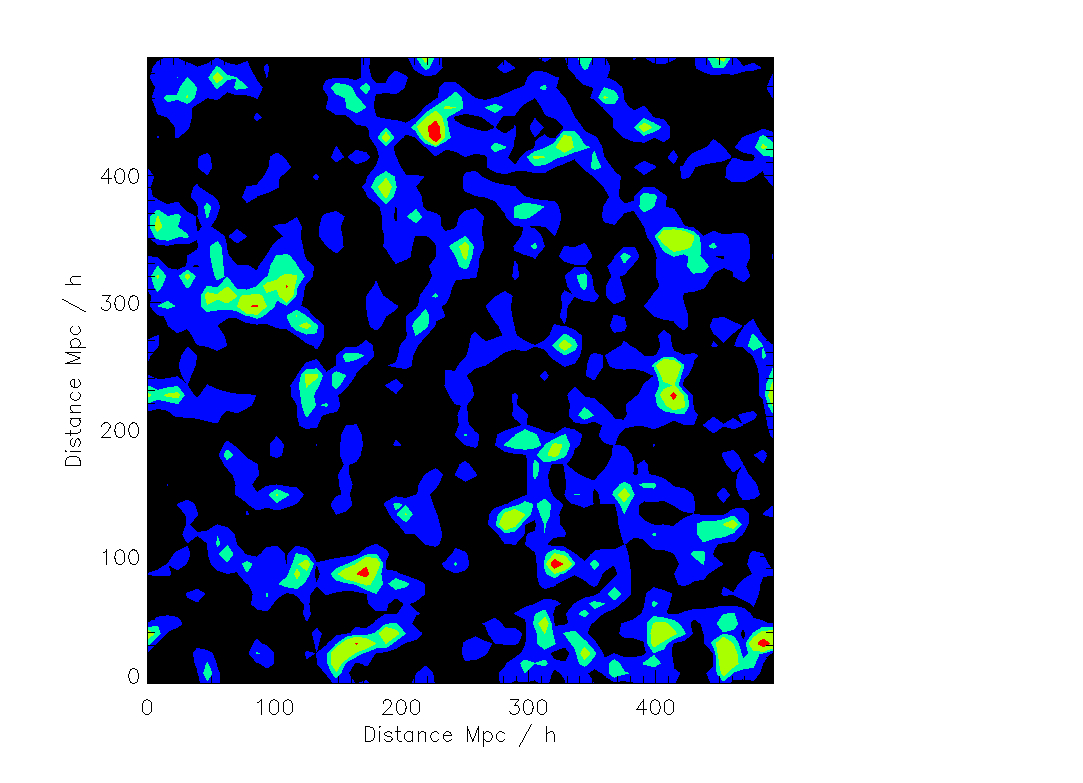
\includegraphics[width=0.49\columnwidth]{./full/gadget/contour/del_contour004}

   \end{center}
\caption{These plots come from the Gadget simulation and show a contour plot of density contrast ($\delta$). The box is $500 \; {\rm Mpc / h}$ on each side. The contour levels are $\delta = -1, 0, 1, 2, 5$.}
\label{fig.gadget_contour}
\end{figure}


\subsubsection{Gaussian smoothing}
Given the magnitude of the over-densities in the initial condition $|\delta|_{\rm initial} \sim 0.3$ we previously suppressed this value by dividing the values across the whole field by 10. This was an arbitrary choice, however in cosmology there is a an accepted standard for smoothing that advocates smoothing the data with a gaussian window with a standard deviation of  $\sigma = 8$ Mpc. It is an accepted standard because, statistically, all structures larger than 8 Mpc are roughly linear.

This method of smoothing was chosen and applied to both the initial density field and to the output density fields. The smoothed initial density field was supplied to the wave-mechanics code for another run of the simulation to be performed.

The smoothing operation is defined in the following way:
\begin{equation}
\rho_{gauss} = \frac{1}{W} \sum_{-\sigma_z}^{\sigma_z} \sum_{-\sigma_y}^{\sigma_y} \sum_{-\sigma_x}^{\sigma_x} \rho_{TSC}\; e^{\left(\frac{-(r-r')^2}{2 \sigma^2} \right)}
\end{equation}

\noindent here $\rho_{gauss}$ is new smooth field and $\rho_{TSC}$ is the density field as generated by the TSC smoothing routine in case of the Gadget outputs. Recall that the TSC routine smooths particle positions onto a uniform grid and hence gives a continuous density field. The weight, $W$, is defined as:
\begin{equation}
W = \sum_{-\sigma_z}^{\sigma_z} \sum_{-\sigma_y}^{\sigma_y} \sum_{-\sigma_x}^{\sigma_x} e^{\left(\frac{-(r-r')^2}{2 \sigma^2} \right)}
\end{equation}

\noindent where it is already assumed that we will truncate the gaussian to a certain precision, in this case 3 standard deviations ($\sigma$). In the simulation performed, a physical length of $500$ Mpc was chosen, and the resolution was $64^3$. This means that one pixel has a length of $7.8$ Mpc hence 3 pixels roughly corresponds to 3 standard deviations.

Figures \ref{fig.gadgauss} \& \ref{fig.wmgauss} show contour plots of over-density, $\delta$, from Gadget and wave-mechanics respectively. The peaks have been well smoothed out by roughly a factor of 6. The contour levels are black for $\delta < 0$ and blue for $\delta \geq 0$. The results for Gadget look almost static over the full run of the simulation but there is some movement within the structure.

The results for wave-mechanics look less random at later times, there are definite structures in the smoothed density fields at late times ($a \sim 1$). In the previous unsmoothed outputs (such as figure \ref{fig.wmhistdc}) long-term structure was not as distinguishable as in these newer results.

The problem seems to have been due to the initial density peaks being too high for our chosen resolution. The maximum over-density peak was $\delta \sim 0.3$ in the original initial conditions, here in the smoothed initial condition it is $\sim 0.05$. The growth of the maximum value of $\delta$ is also much slower and reaches a maximum of $\delta = 9.1$ in the final output. This is comparable to the unsmoothed initial density field of wave-mechanics in the previous section. The big improvement now is that the outputs from wave-mechanics look closer to those from Gadget (after gaussian smoothing).

Like previous results we can see regions of multi-streaming which resemble an interference pattern. The outputs from wave-mechanics are noticeably less clean but this isn't a surprise given the added complexity inherent in wave-mechanics and the fact that we are now dealing with a continuous density field.


\begin{figure}[htb]
   \begin{center}
     %\leavevmode
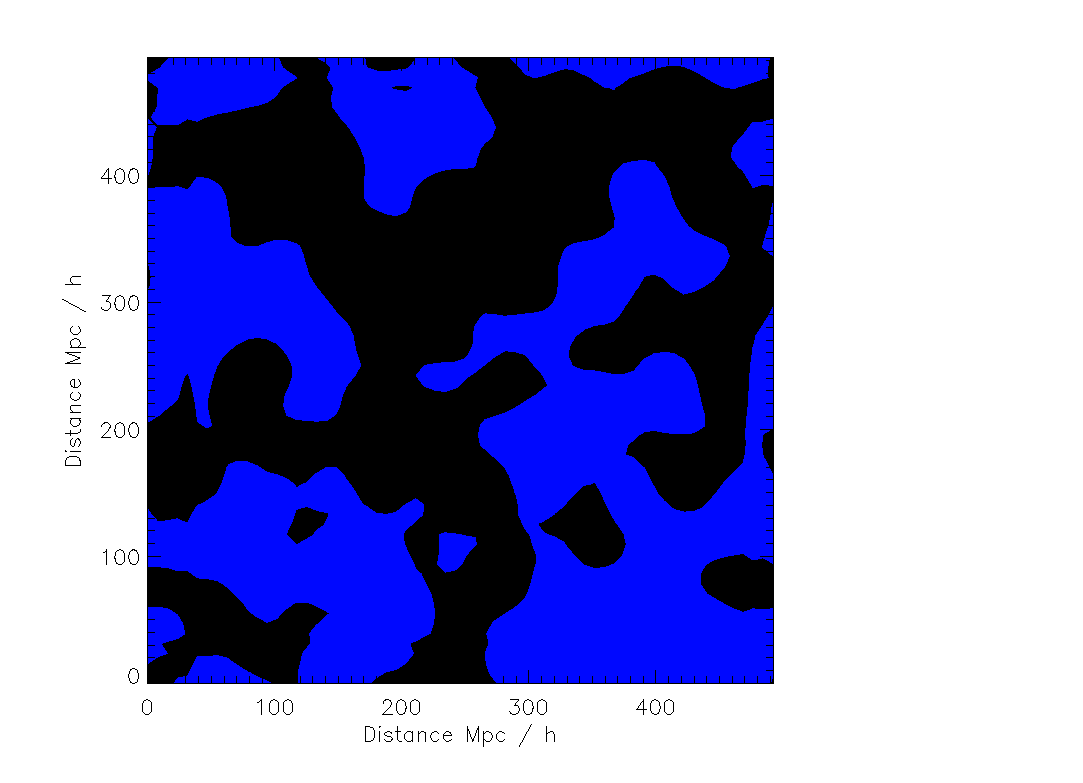
\includegraphics[width=0.45\columnwidth]{./full/gadget/gaussian/0000_del_contour}
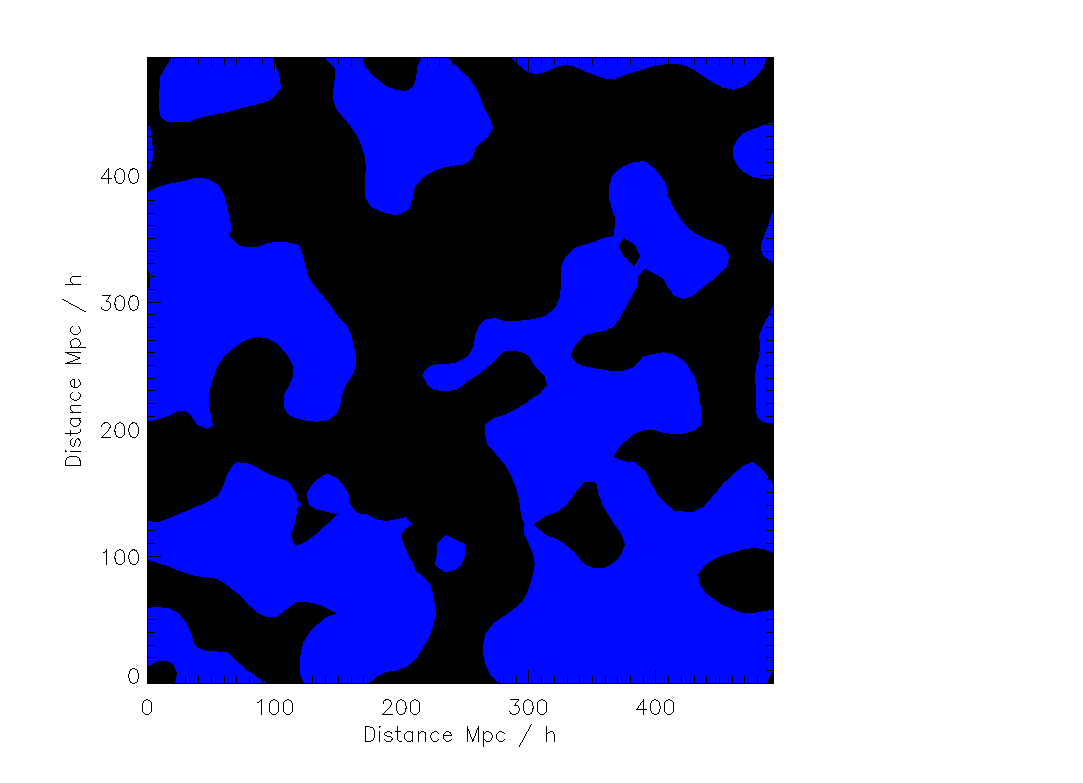
\includegraphics[width=0.45\columnwidth]{./full/gadget/gaussian/000_del_contour.eps}
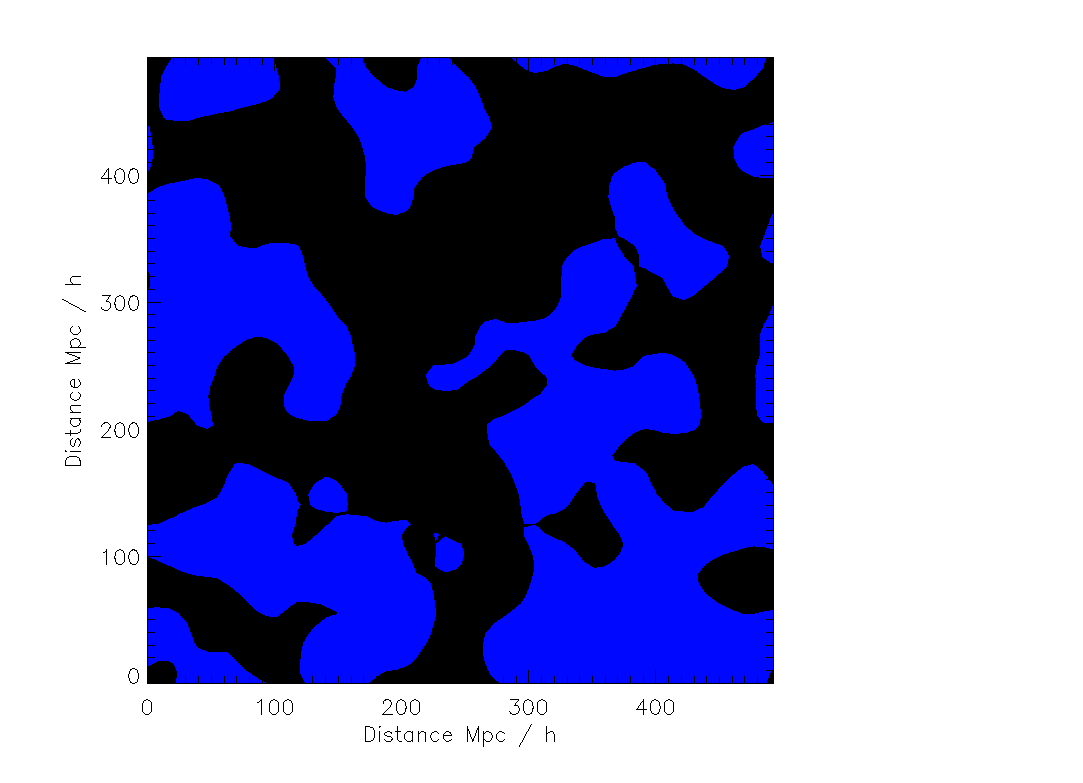
\includegraphics[width=0.45\columnwidth]{./full/gadget/gaussian/001_del_contour.eps}
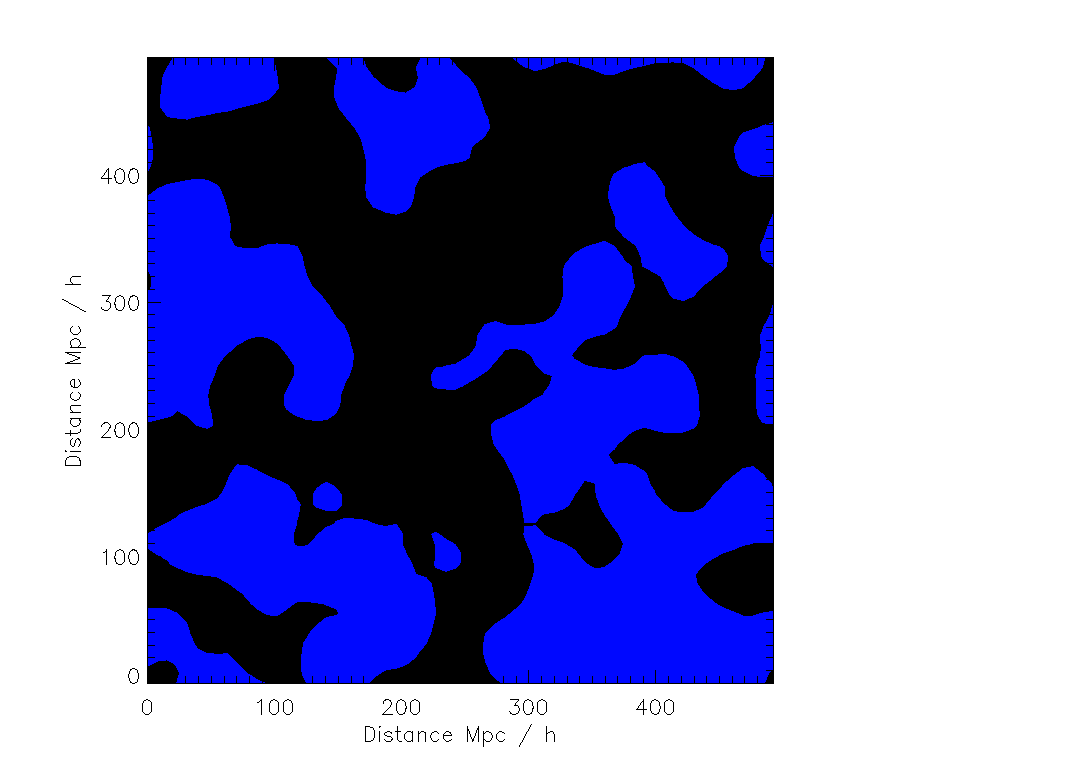
\includegraphics[width=0.45\columnwidth]{./full/gadget/gaussian/002_del_contour.eps}
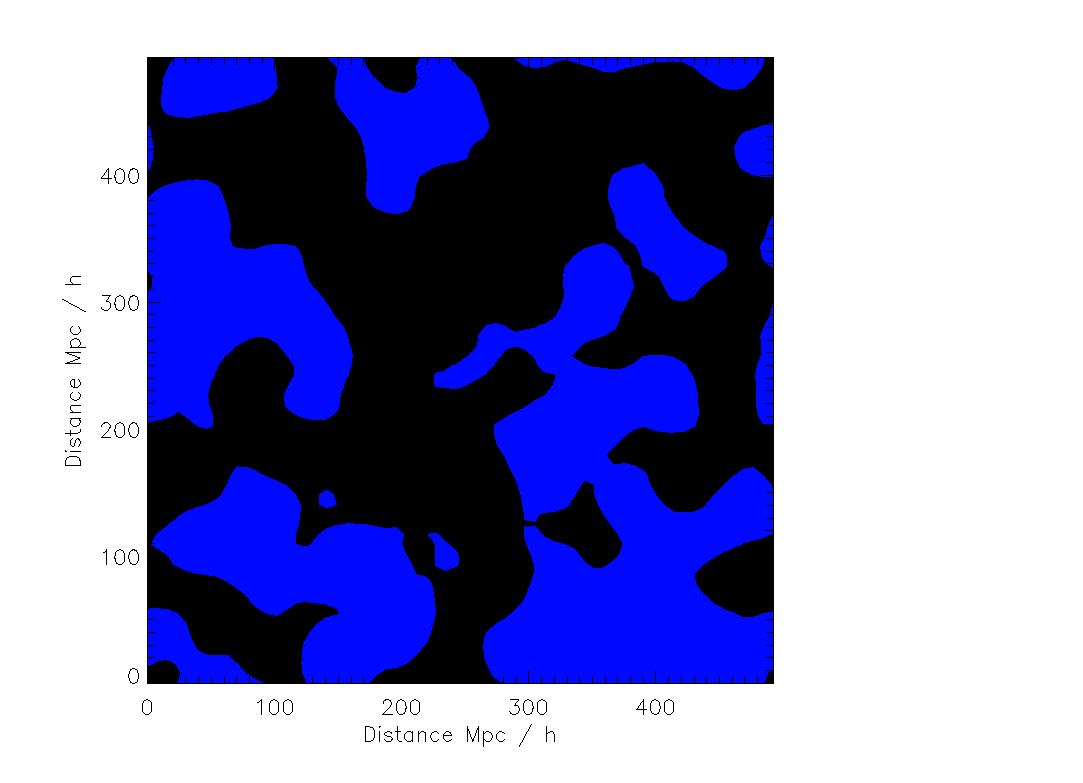
\includegraphics[width=0.45\columnwidth]{./full/gadget/gaussian/003_del_contour.eps}
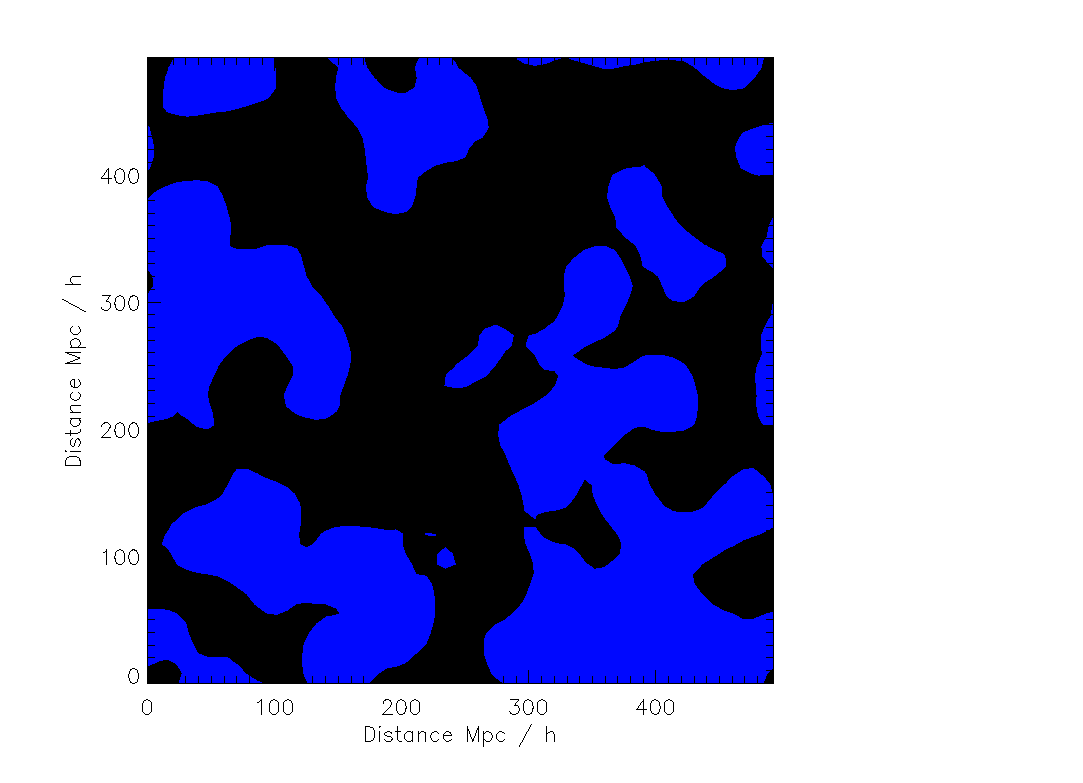
\includegraphics[width=0.45\columnwidth]{./full/gadget/gaussian/004_del_contour.eps}

   \end{center}
\caption{This series of contour plots shows the previously seen Gadget outputs for over-density ($\delta$) after gaussian smoothing has been applied. $z = 32, 3, 2, 1, 0.5, 0.05$. The contour levels are black for $\delta < 0$ and blue for $\delta \geq 0$.}
\label{fig.gadgauss}
\end{figure}


\begin{figure}[htb]
   \begin{center}
     %\leavevmode
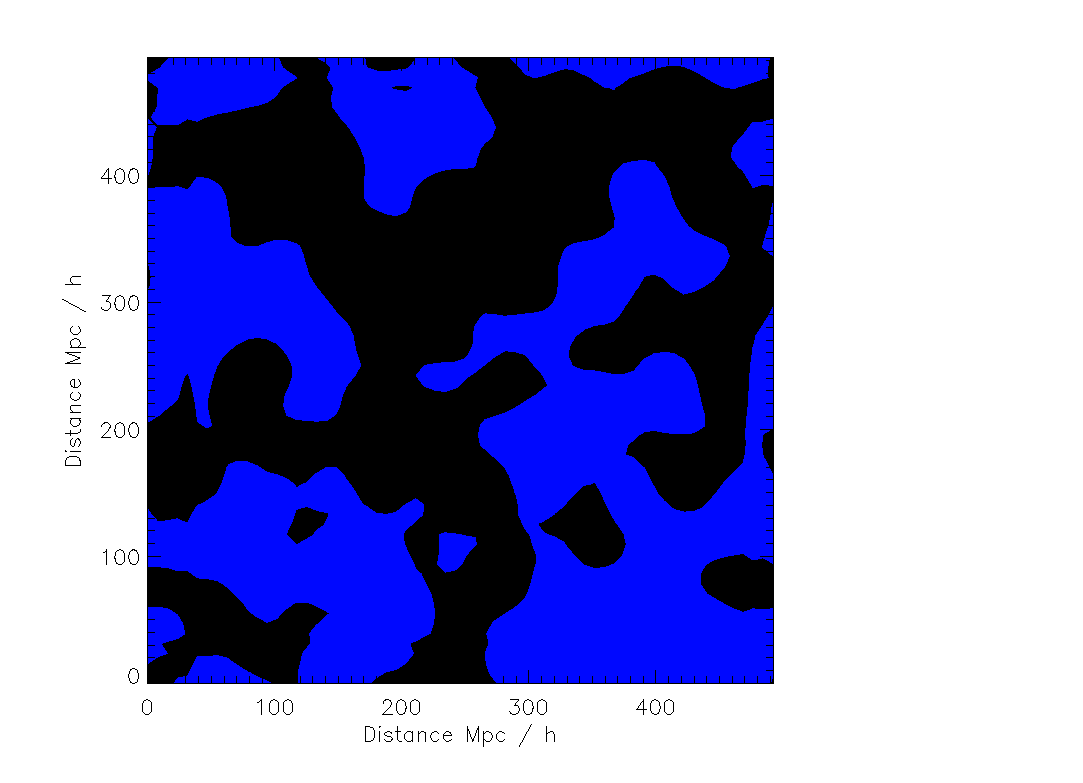
\includegraphics[width=0.45\columnwidth]{./full/wm64/rho_gauss/00000_del_contour}
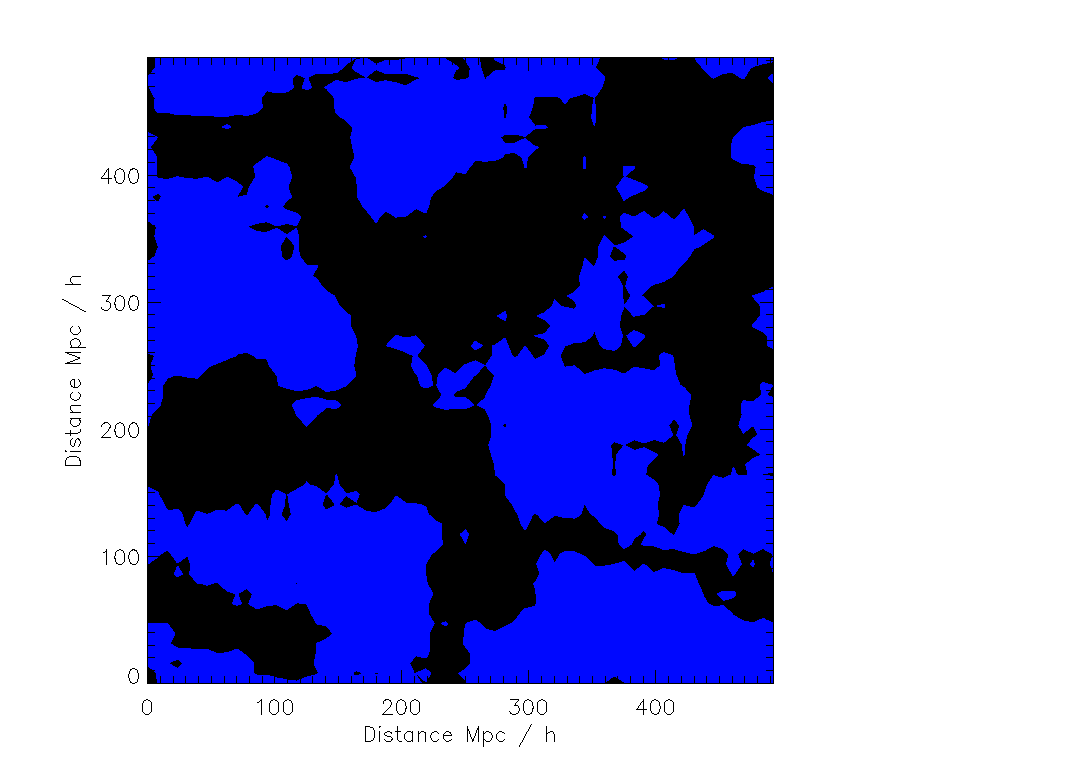
\includegraphics[width=0.45\columnwidth]{./full/wm64/rho_gauss/00200_del_contour}
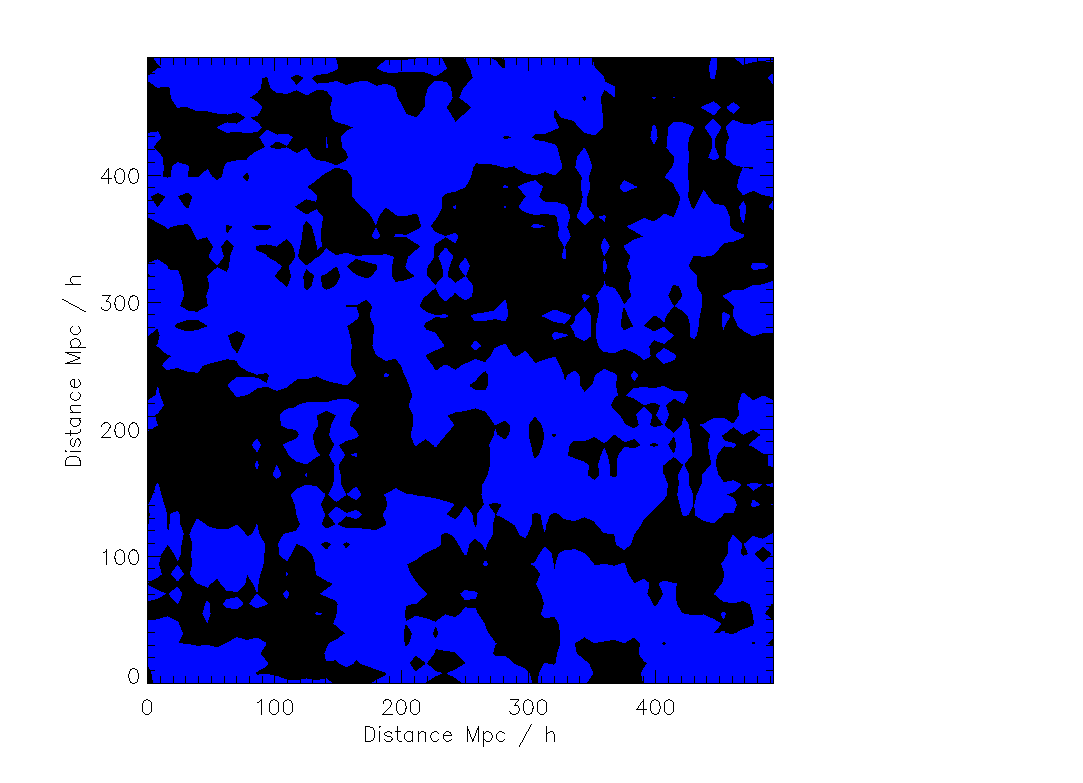
\includegraphics[width=0.45\columnwidth]{./full/wm64/rho_gauss/01000_del_contour}
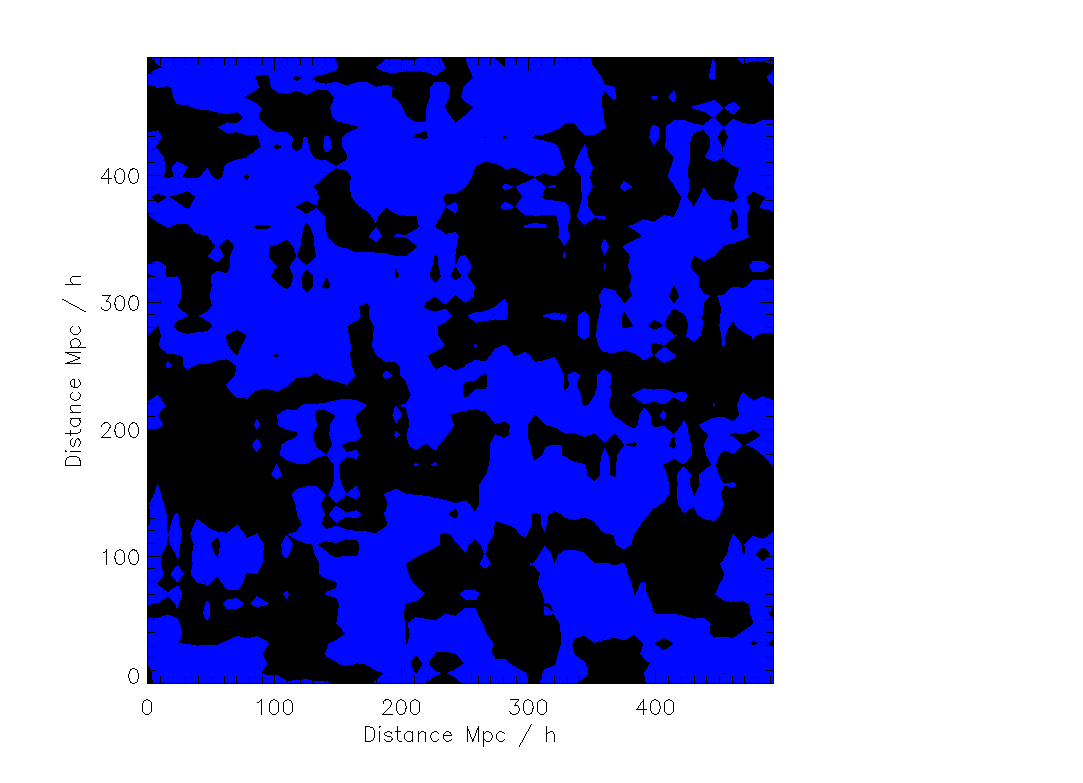
\includegraphics[width=0.45\columnwidth]{./full/wm64/rho_gauss/02000_del_contour}
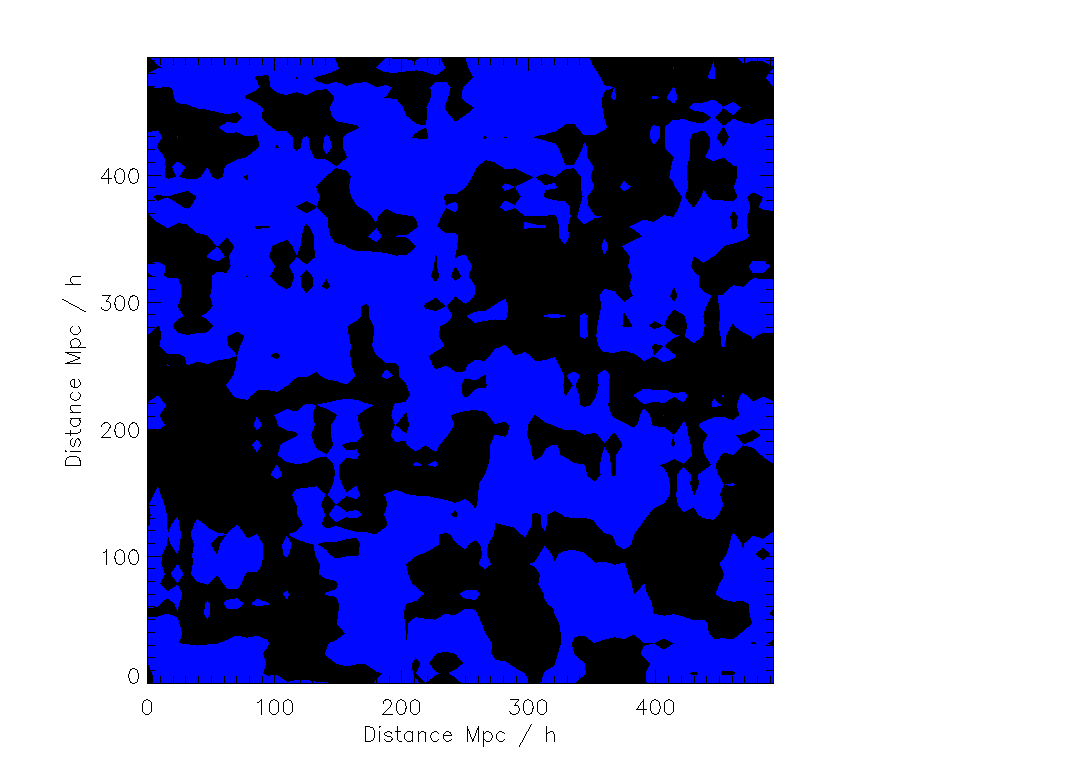
\includegraphics[width=0.45\columnwidth]{./full/wm64/rho_gauss/03000_del_contour}
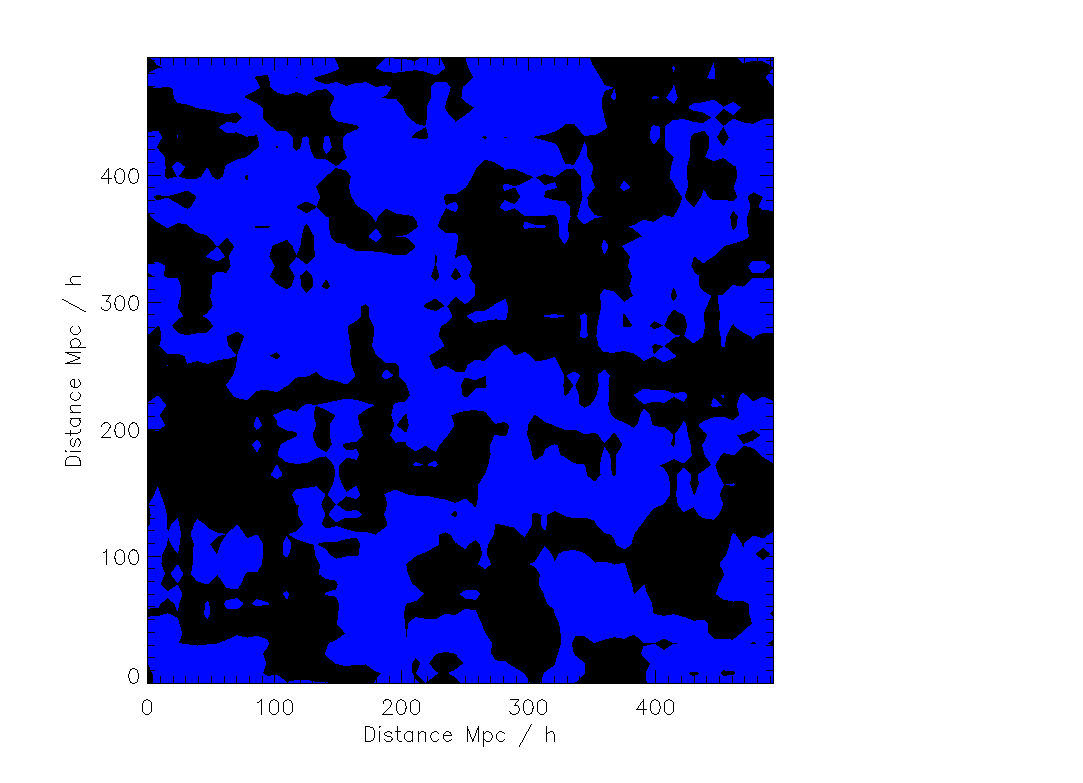
\includegraphics[width=0.45\columnwidth]{./full/wm64/rho_gauss/03500_del_contour}

   \end{center}
\caption{This series of contour plots shows the previously seen wave-mechanics outputs for over-density ($\delta$) after gaussian smoothing has been applied. The outputs at $t = 0, 200, 1000,$ $2000, 3000, 3500$ ($a = 0.03125,0.038,$ $0.085,0.23, 0.63, 1.03$). The contour levels are black for $\delta < 0$ and blue for $\delta \geq 0$. }
\label{fig.wmgauss}
\end{figure}


\subsubsection{Robustness of results --- conserved quantities}
\label{ch_5_robust}
Given the high variability of density peaks spatially, it is not apparent that the code is well-behaved. Hence it is worth performing consistency checks, such as plotting histograms but as mentioned through out this thesis we are ideally concerned with conserved physical quantities. The stability and robustness of the wave-mechanics code is verified by the conservation of mass and momentum. Over the whole simulation from the initial conditions until redshift $z = 0$ (3500 timesteps), the variation of mass is less than 7 significant figures. While momentum conservation (denoted by $P$) is only slightly worse but an unnoticeable effect in the simulation. Together these two conserved quantities dictate that energy must also be conserved, as is required from a symplectic integration scheme. Figure \ref{fig.conserve} shows how these quantities vary over the course of the simulation.

The quantities were calculated as follows:

\begin{eqnarray}
M_{\rm total} &=& \int^V \psi \psi^* \; dx^3 \\
P_{\rm total} &=& \int^V |\psi^* \nabla \psi|^2 \; dx^3
\end{eqnarray}

Naturally, these quantities have regimes where they are not conserved and the code is has huge errors. The regimes of stability are dictated by the resolutions lengths $dx$ and $dt$ as with any finite difference (or finite element) code. However, there is an additional parameter that dictates stability: $\nu$. When $\nu$ is relatively large (as dictated by choice of $n_g$, the number of gridpoints per side) then the dispersion of the wavefunction is higher but if this value is too large then the wavefunction allows for matter to move too quickly. When this happens, mass and momentum are no longer conserved.


\begin{figure}[htb]%[tp]%[htb]
   \begin{center}
    % \leavevmode
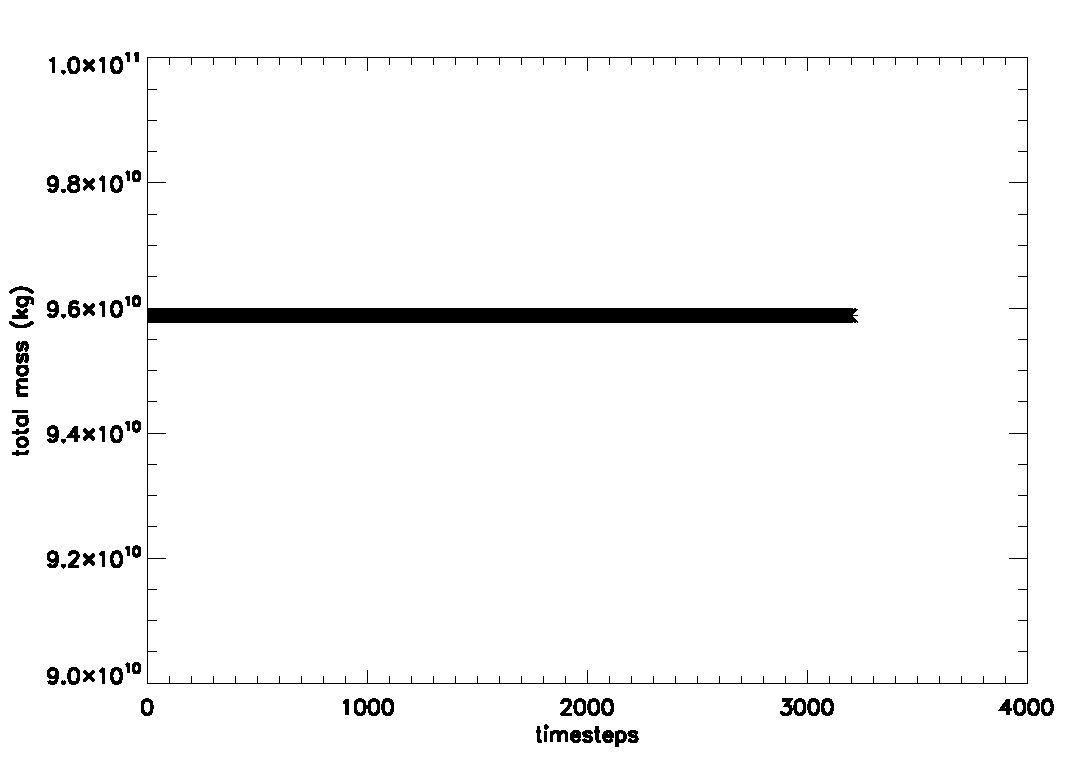
\includegraphics[width=0.49\columnwidth]{./full/wm64/tot_mass3200}
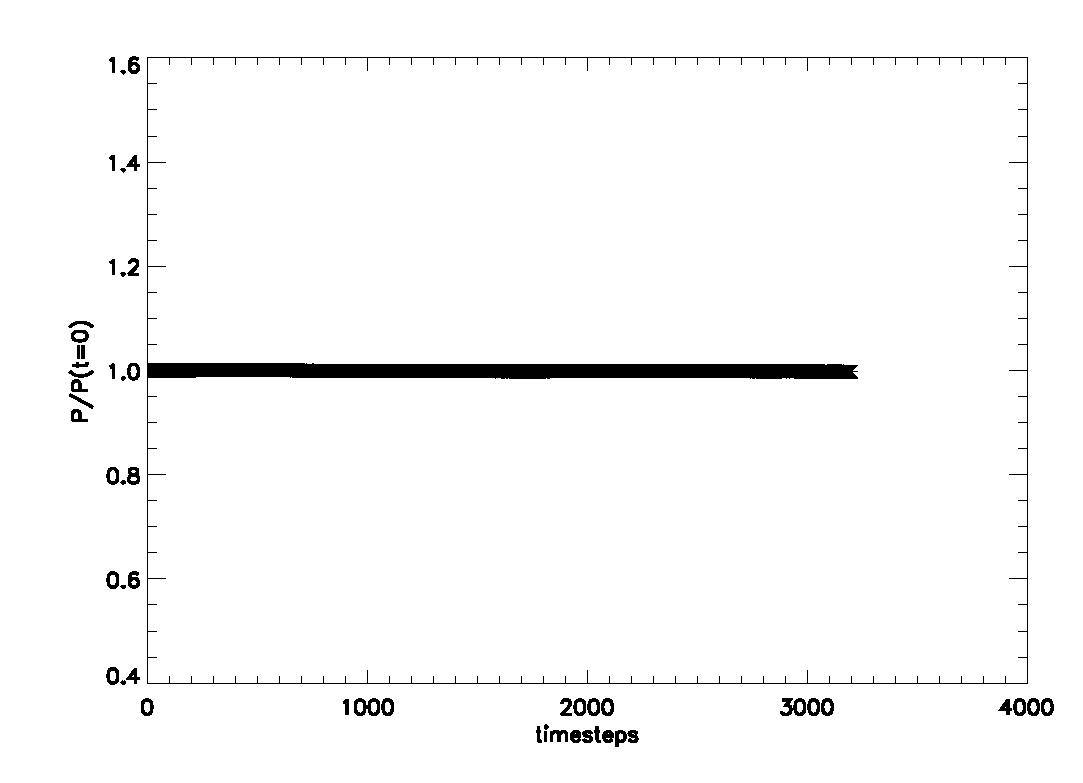
\includegraphics[width=0.49\columnwidth]{./full/wm64/normed_tot_mom3200}
   \end{center}
\caption{The conservation of total mass (left) and total momentum (right) over time in the wave-mechanics code. The flatness of the distribution shows that the quantities do not vary significantly over time.}
\label{fig.conserve}
\end{figure}

\section{Velocity \& Vorticity}
The main focus of this section is to show the comparison between  the ``industry standard'' code, Gadget, and our own wave-mechanics code. In figure \ref{fig.gadvel} we present the velocity in the form of histograms of the $x$ component of velocity. From symmetry we require that the other velocity components, $y \; \& \; z$, have the same shape (height and width) at all output times. The histograms of the other velocity components confirm this is the case; for brevity, those plots have been omitted from this thesis.

Overplotted on each of the Gadget velocity histograms is that of a theoretical gaussian with the same amplitude and standard deviation. We can see very good agreement between the data and the theoretical gaussian. The velocity data from the Gadget output files requires a simple scaling in order to calculate the real physical velocities: $v_{real} = \sqrt{a} v_{code}$ (km/s).

The velocity from the wave-mechanics code can be calculated using the probability current as given by equation \ref{eqn_j}. This technique was presented as the big difference between my FPA code that that of Short \citep{bib_short}. We have shown that the velocity from the probability current is consistent with the results of Short who used a phase unwrapping technique. As shown in Chapter \ref{ch_3}, we can use a simpler form of the probability current:

\begin{equation}
\underline{v} = \frac{\hbar}{m} \Im\left(\frac{\nabla \psi}{\psi}\right)
\end{equation}

Figure \ref{fig.wmvel} shows a series of graphs of the $x,y$ components of velocity (at a fixed value of $z$) and correspond to the density and over-density plots from the wave-mechanics code shown above (figures \ref{fig.wmrho} \& \ref{fig.delta_contour}, respectively). The velocities at earlier times appear isotropic as expected and of roughly equal magnitude (with a gaussian distribution).

For comparison with the Gadget histograms (\ref{fig.gadvel}), I also provide histograms for the $x$ component of velocity from the wave-mechanics code. It also appears as a gaussian at earlier times by evolves in a slightly different way to Gadget, the tails of the distributions become much longer than they are in Gadget. Also, I must point out that this data has been smoothed using a gaussian smoothing routine. The effect of this smoothing makes the distribution shorter and fatter, both pre- and post- smoothing distributions are however gaussian. This partly what we expect: we expect a gaussian distribution but it is not entirely obvious why the wave-mechanics code produces a distribution with longer tails. This likely to be a fundamental issue of wave-mechanics rather than our specific implementation.

Worth noting is that the range of velocities calculated over time is greater in the wave-mechanics code than in Gadget. Strangely, the initial velocities that we calculated in wave-mechanics is not the same as those in the Gadget code. Currently, this is an unsolved problem and may be due to how the initial wavefunction is constructed: $\psi \propto \rho^{1/2} \exp(i\Phi_g)$. Which uses the gravitational potential rather than the velocity potential. Physically, the two fields are not the same but at early times in the Universe are believed to be linearly proportional to each other. That is to say that this problem is unexpected and the scaling between the two fields may not be the problem. We may then have to consider if the calculation of the gravitational potential from the density field is somehow deficient. Not only does this affect the initial velocity field but it affects the dynamics of our system and hence could be a source of a large systematic error.

The velocity results are contradictory with the fact that momentum is conserved (as just shown in figure \ref{fig.conserve}) for the duration of the simulation. To the best of our knowledge the calculations are correct but unfortunately we have not found the root error of this conundrum.

The initial density field is identical to that of Gadget hence the source of discrepancy has to come from either (1) the scaling of gravitational potential to the velocity potential or (2) the calculation of the velocity field is incorrect. The latter might suggest that an additional constant scaling factor must be added to the results. This would force the width of the velocity distribution from wave-mechanics to be identical to that of Gadget, this would also mean that subsequent outputs of velocity will be wider too. At later times this would provide an even greater discrepancy between the maximum and minimum velocities of wave-mechanics versus that of Gadget.


The following table provides the key values of the velocity distribution (over time) from the wave-mechanics code:

\vspace*{1cm}
\begin{center}
\begin{tabular}{|c|c|c|c|c|c|c|}
  \hline
  t = & 0 & 200 & 1000 & 2000 & 3000 & 3500 \\
  a = & 0.03125 & 0.038 & 0.085 & 0.23 & 0.63 & 1.03 \\
  z = & 31 & 25.3 & 10.8 & 3.3 & 0.6 & -0.03 \\  \hline
  max$[V_x]$ & 26.9 & 32.8& 277.9& 1824& 5332& 5768 \\
  min$[V_x]$ & -35.4&-43.6&-261.1&-4711&-4571& -7452 \\
  mean$[V_x]$ & -3.7&-4.5 &-9.12 &-29.32&-65.24&-165  \\
  $\sigma[V_x]$ & 7.5&9.2 &30.79 &173.8& 398.9& 687 \\
  \hline
\end{tabular}
\end{center}
\vspace*{1cm}

\noindent As previously stated, the other velocity components $y, z$ are roughly the same as the $x$ component. For brevity the other components are omitted from the table. The quantity $\sigma(V_x)$ in the table is the standard deviation of velocity.

The table indicates that there is a net motion in the $x$ direction, this is also true of the other components. This is worrying as it suggests that the simulation is experiencing a net bulk motion, which will look like an external force is acting upon the system. This is undesirable but hopefully not an unsolvable problem. In this work we do not have enough time to investigate the matter and will have to leave it open for future work.

\begin{figure}[htb]
   \begin{center}
     %\leavevmode
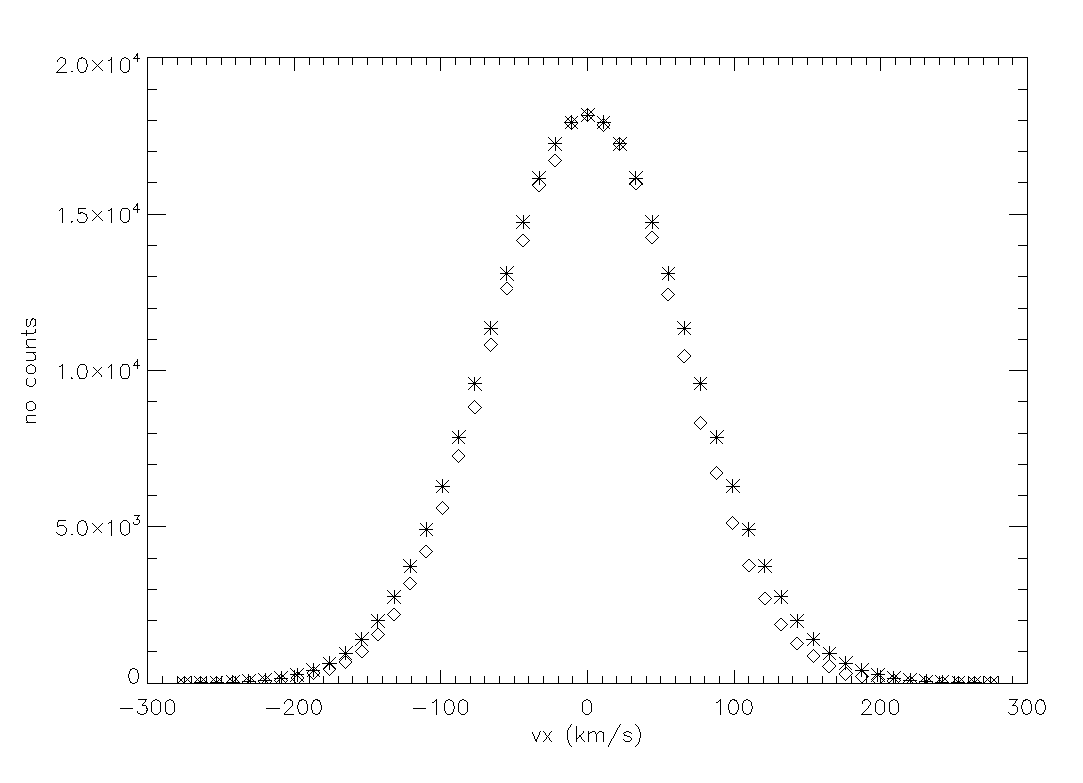
\includegraphics[width=0.49\columnwidth]{./full/gadget/vel/vx_h_hist_0000_z_}
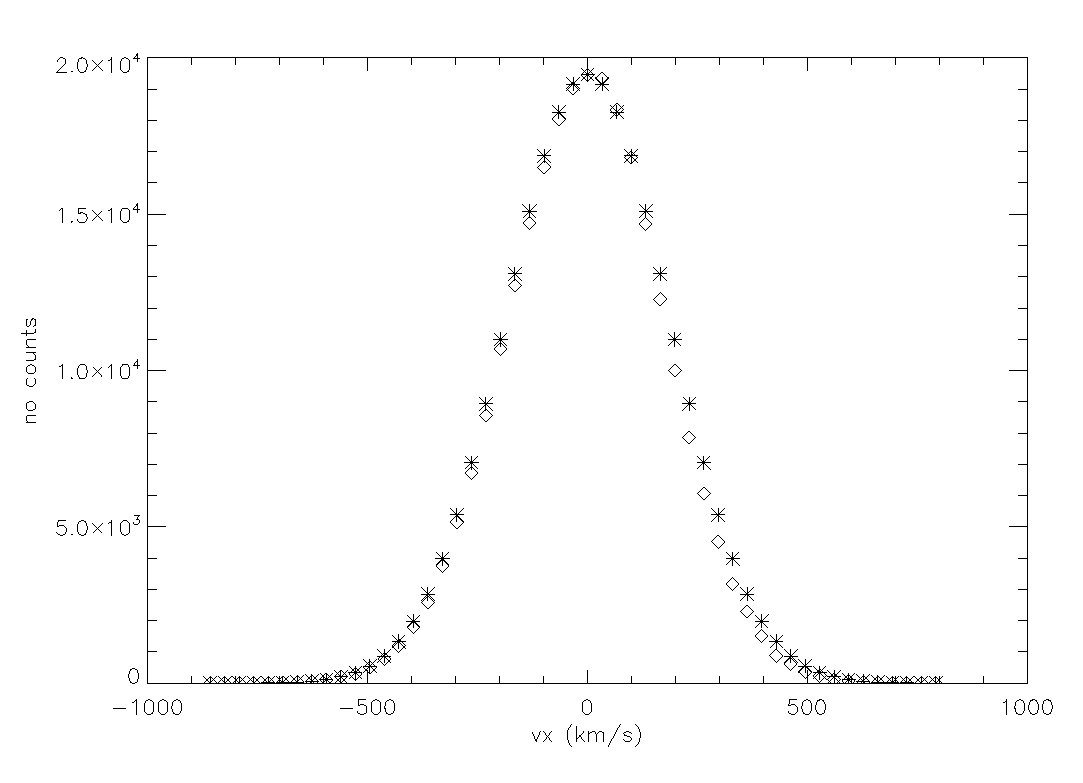
\includegraphics[width=0.49\columnwidth]{./full/gadget/vel/vx_h_hist_000_z_}
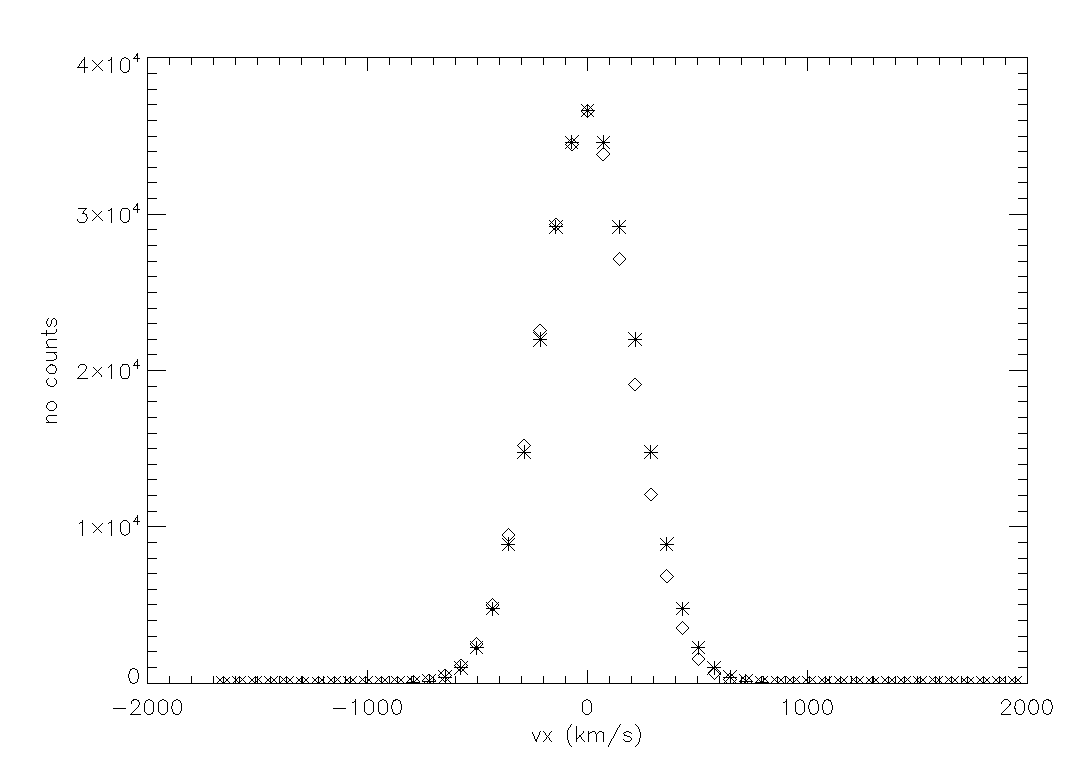
\includegraphics[width=0.49\columnwidth]{./full/gadget/vel/vx_h_hist_001_z_}
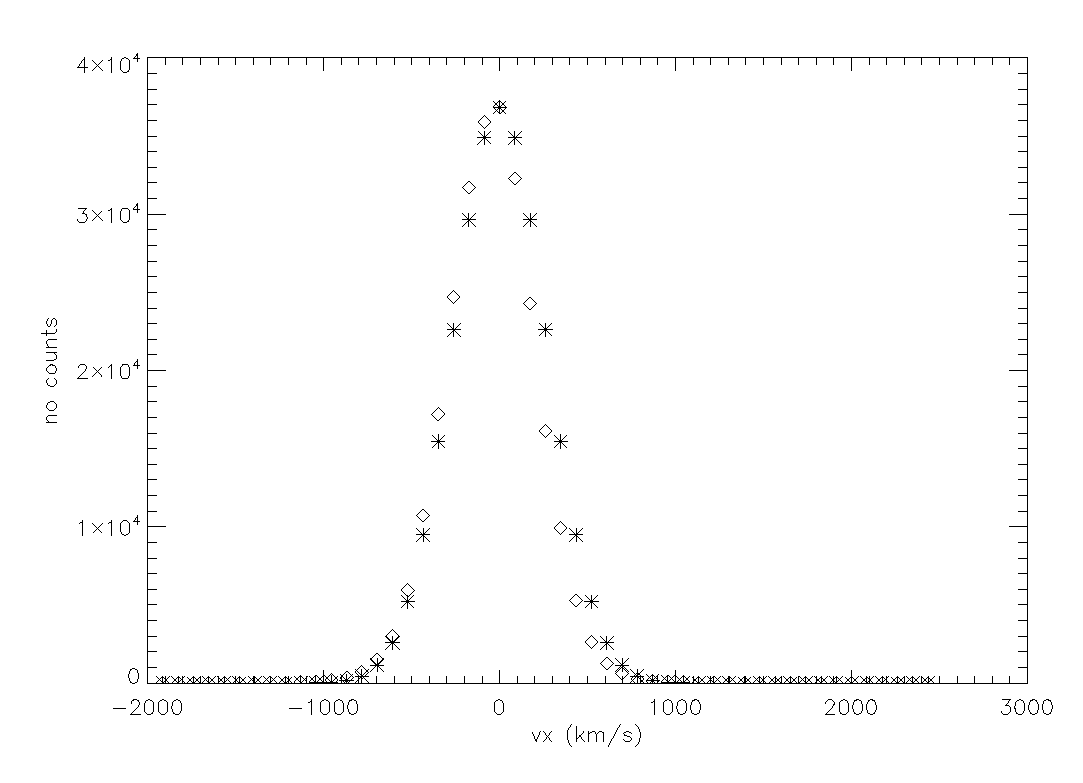
\includegraphics[width=0.49\columnwidth]{./full/gadget/vel/vx_h_hist_002_z_}
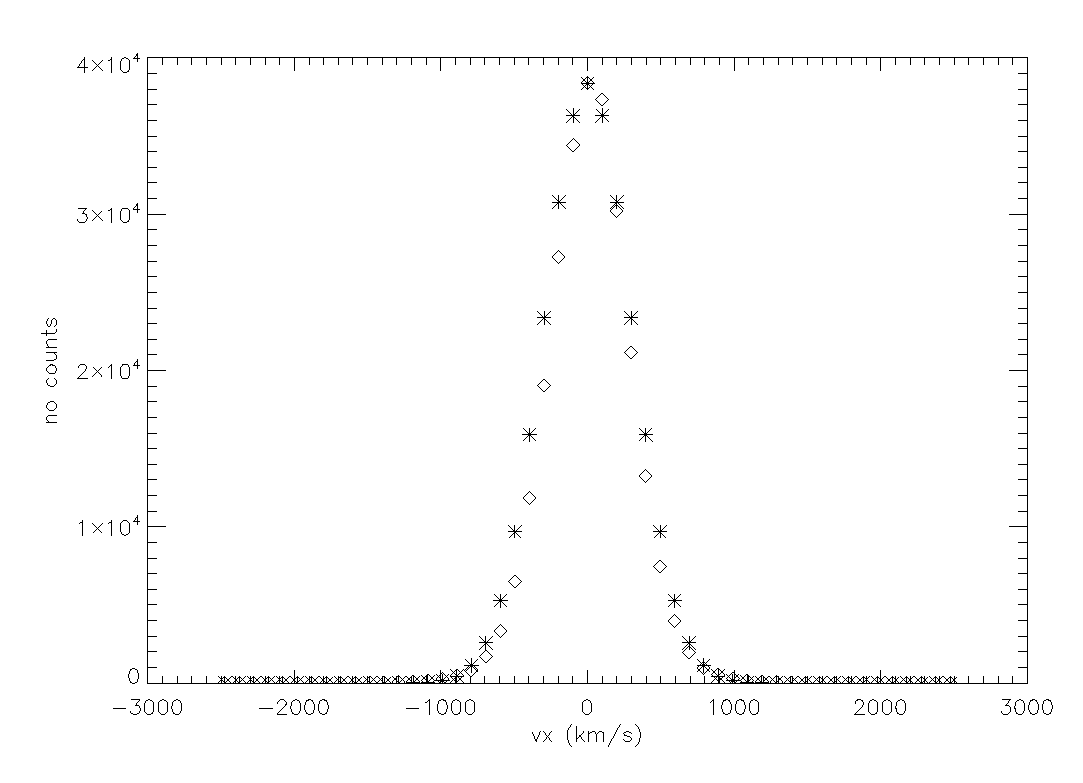
\includegraphics[width=0.49\columnwidth]{./full/gadget/vel/vx_h_hist_003_z_}
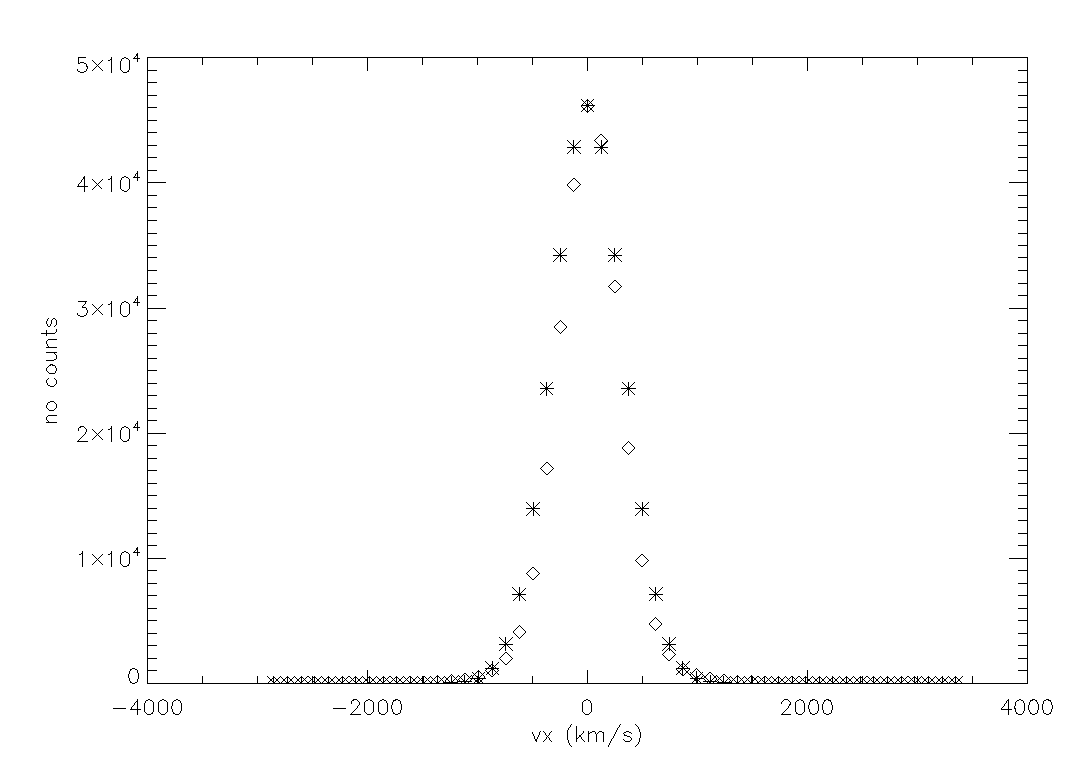
\includegraphics[width=0.49\columnwidth]{./full/gadget/vel/vx_h_hist_004_z_}
   \end{center}
\caption{These plots show a histogram of the $V_x$ component of velocity from the Gadget code. The other velocity components are essentially the same. Overplotted is a theoretical gaussian, shown as asterisks, with the same standard deviation (calculated from the outputted velocity data, shown as diamonds). The times shown are at redshifts: $z = 31, 3, 2, 1, 0.5, 0.05$.}
\label{fig.gadvel}
\end{figure}

\begin{figure}[htb]
   \begin{center}
     %\leavevmode

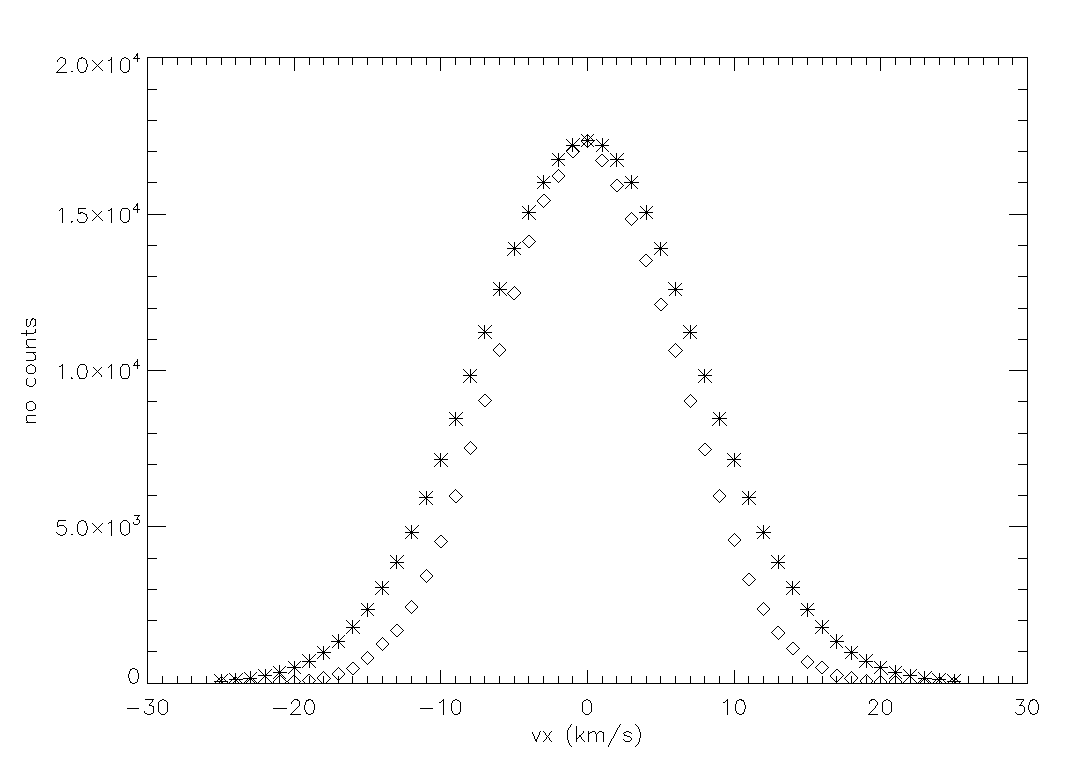
\includegraphics[width=0.49\columnwidth]{./full/wm64/vel/r00000_vxg_hist}
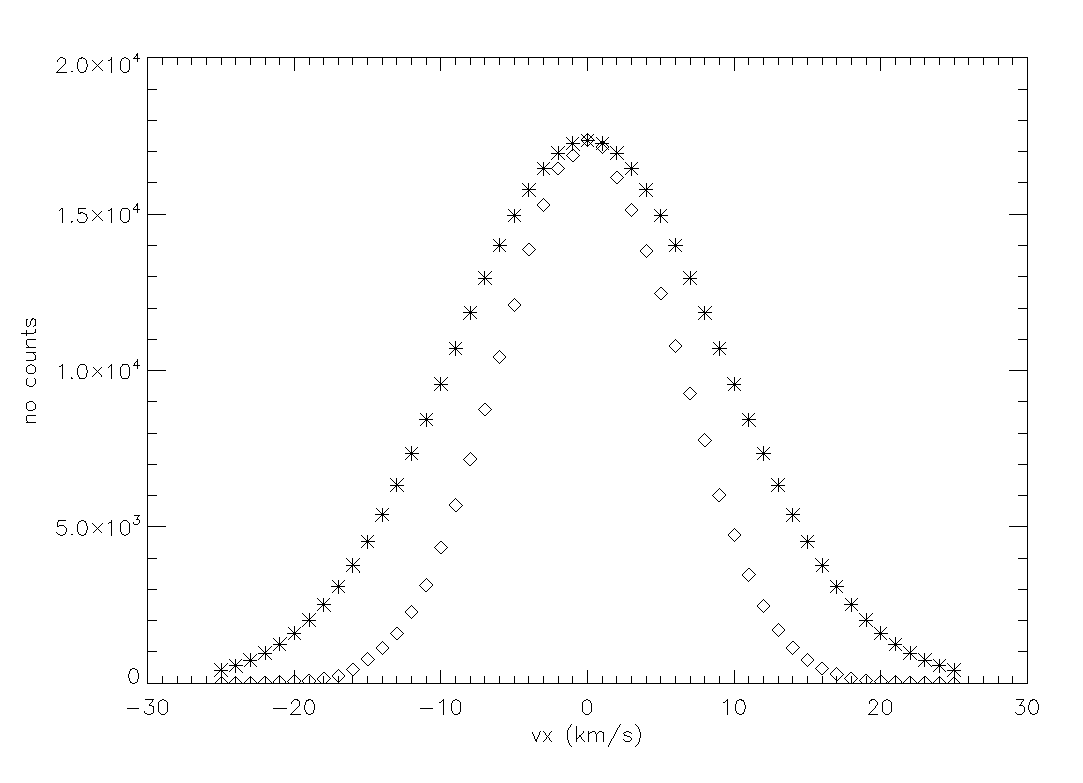
\includegraphics[width=0.49\columnwidth]{./full/wm64/vel/r00200_vxg_hist}
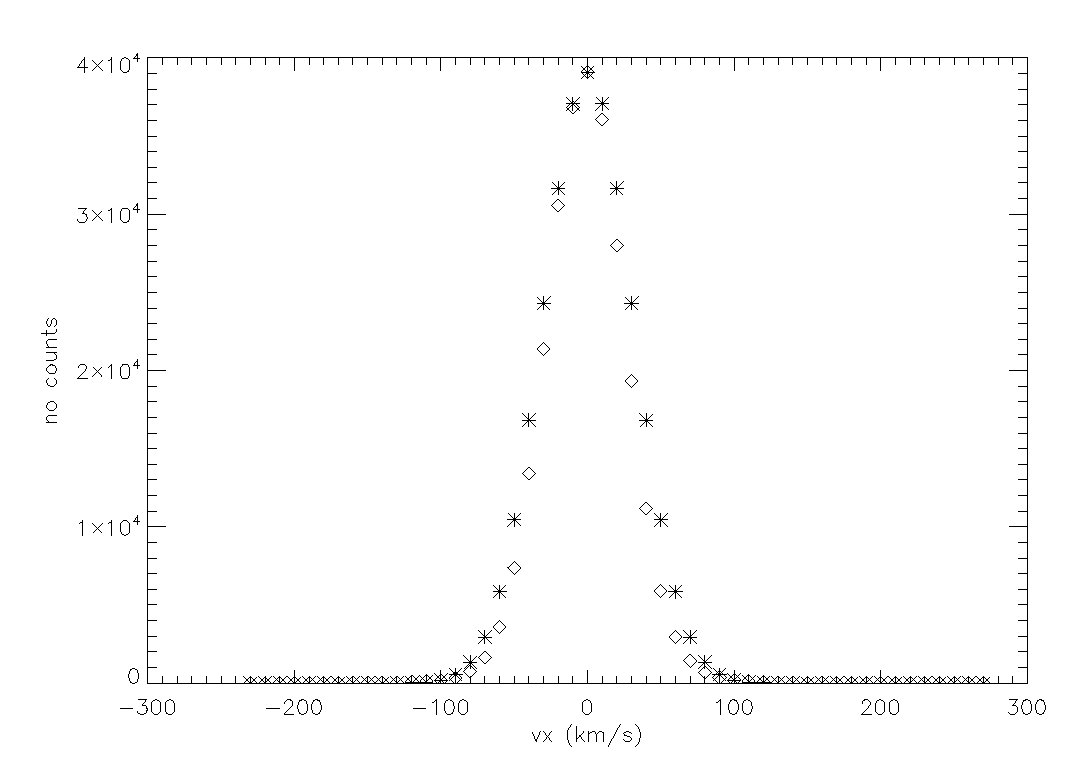
\includegraphics[width=0.49\columnwidth]{./full/wm64/vel/r01000_vxg_hist}
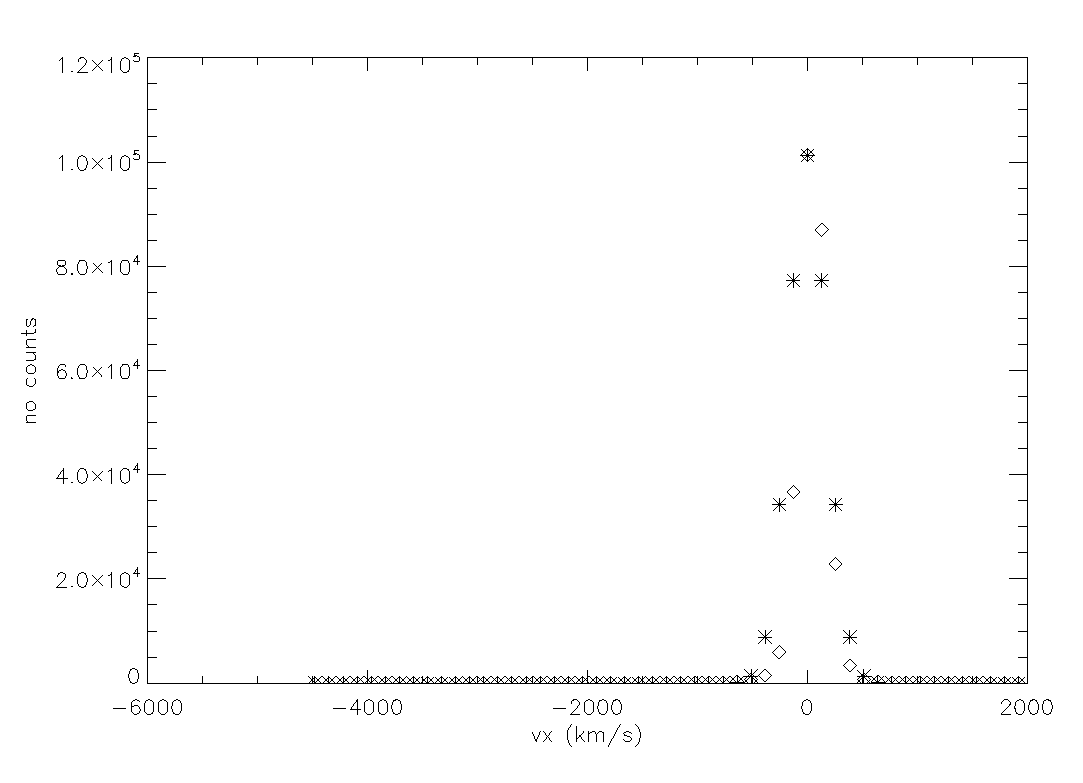
\includegraphics[width=0.49\columnwidth]{./full/wm64/vel/r02000_vxg_hist}
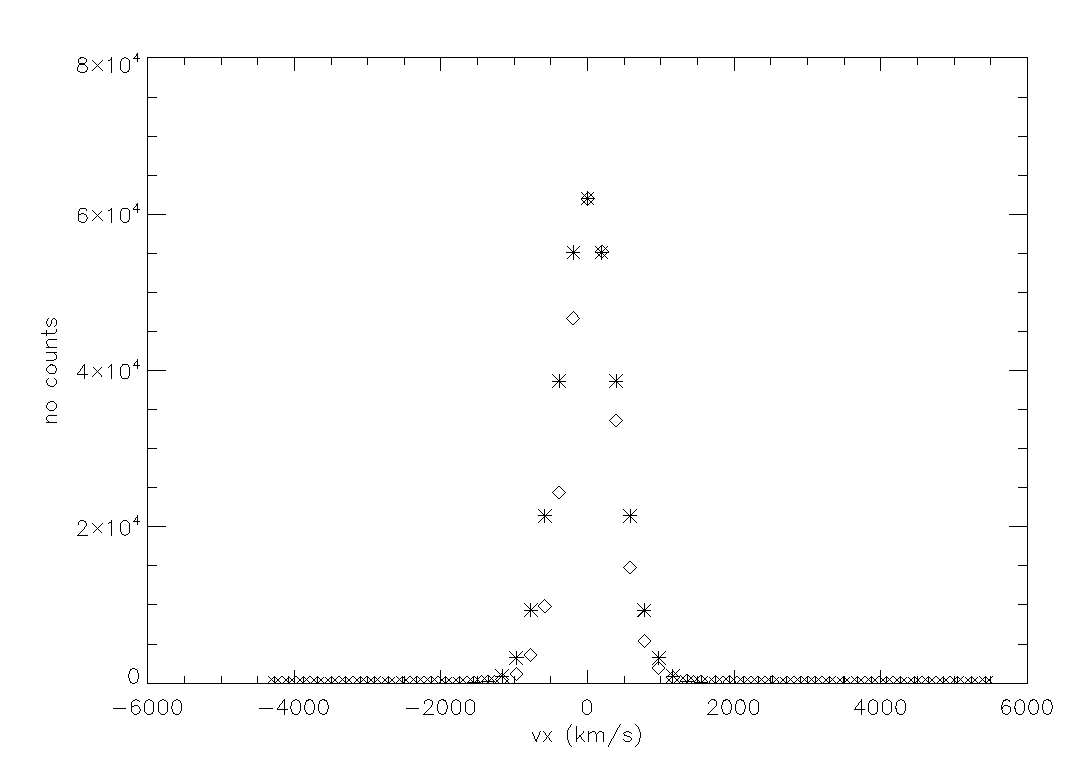
\includegraphics[width=0.49\columnwidth]{./full/wm64/vel/r03000_vxg_hist}
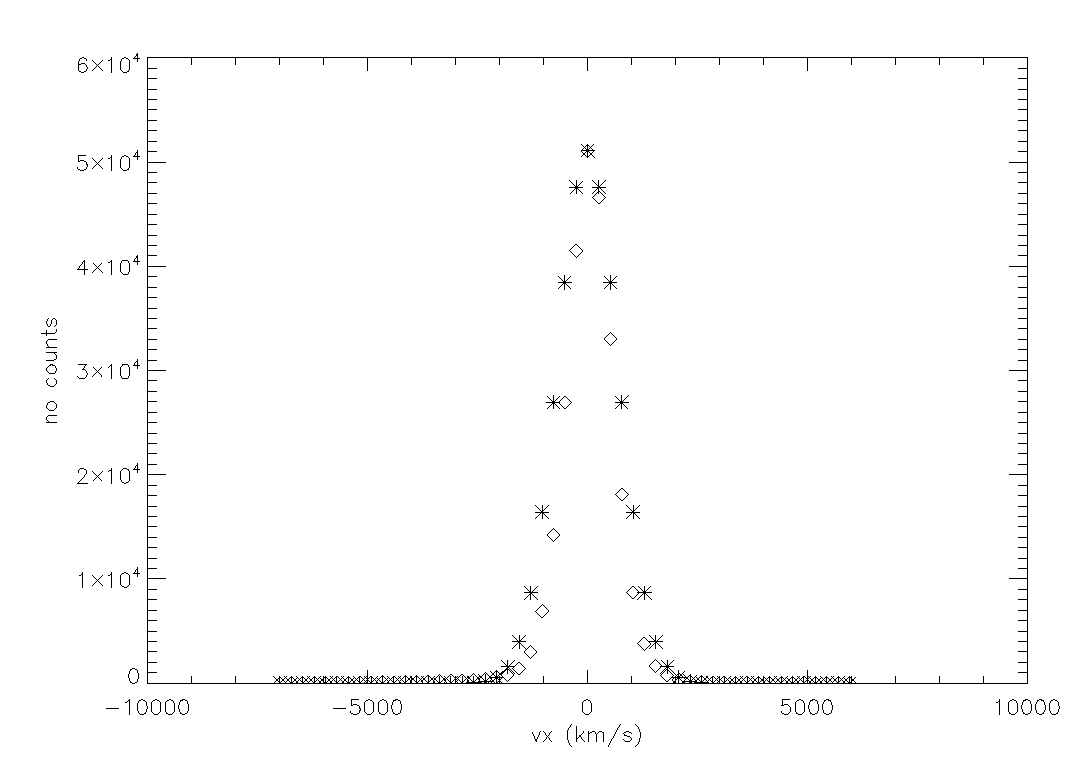
\includegraphics[width=0.49\columnwidth]{./full/wm64/vel/r03500_vxg_hist}

   \end{center}
\caption{These plots show a histogram of the $V_x$ component of velocity from the wave-mechanics code. The other velocity components are essentially the same. Overplotted is a theoretical gaussian, shown as asterisks, with the same standard deviation (calculated from the outputted velocity data, shown as diamonds). As before, the histograms are at times of $t = 0, 200, 1000,$ $2000, 3000, 3500$ ($a = 0.03125,0.038,$ $0.085,0.23, 0.63, 1.03$)}
\label{fig.whvel}
\end{figure}

\begin{figure}[htb]
   \begin{center}
     %\leavevmode

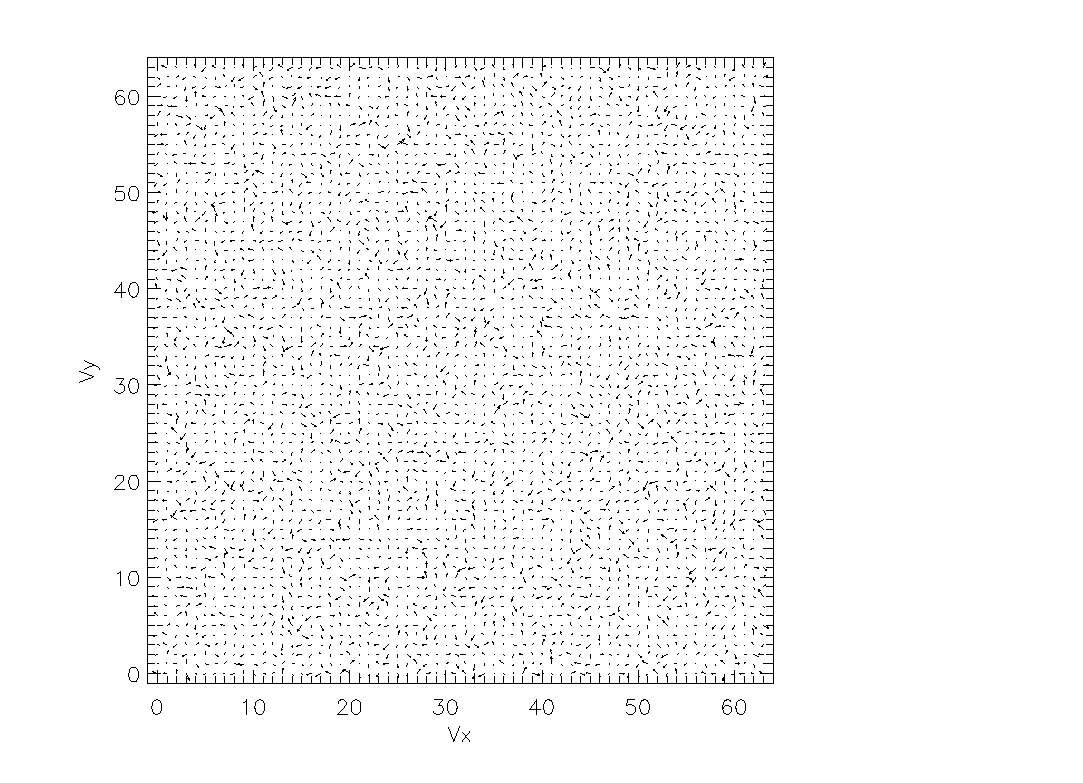
\includegraphics[width=0.49\columnwidth]{./full/wm64/vel/r00000_vel_xy_field}
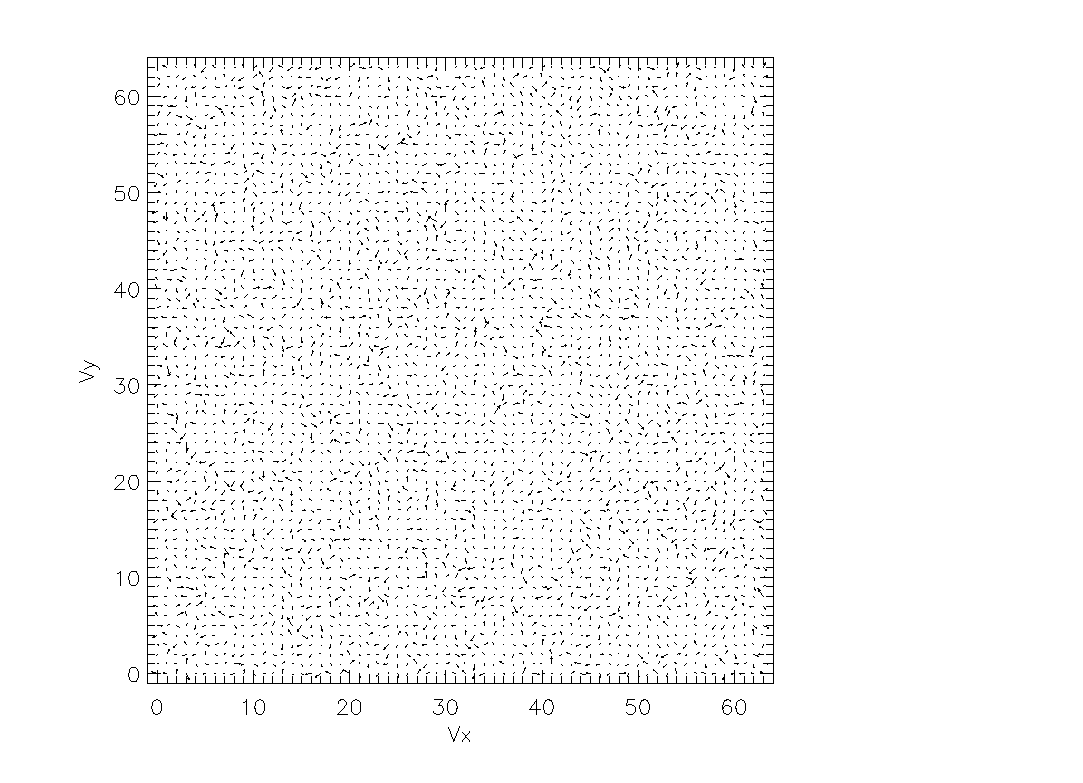
\includegraphics[width=0.49\columnwidth]{./full/wm64/vel/r00200_vel_xy_field}
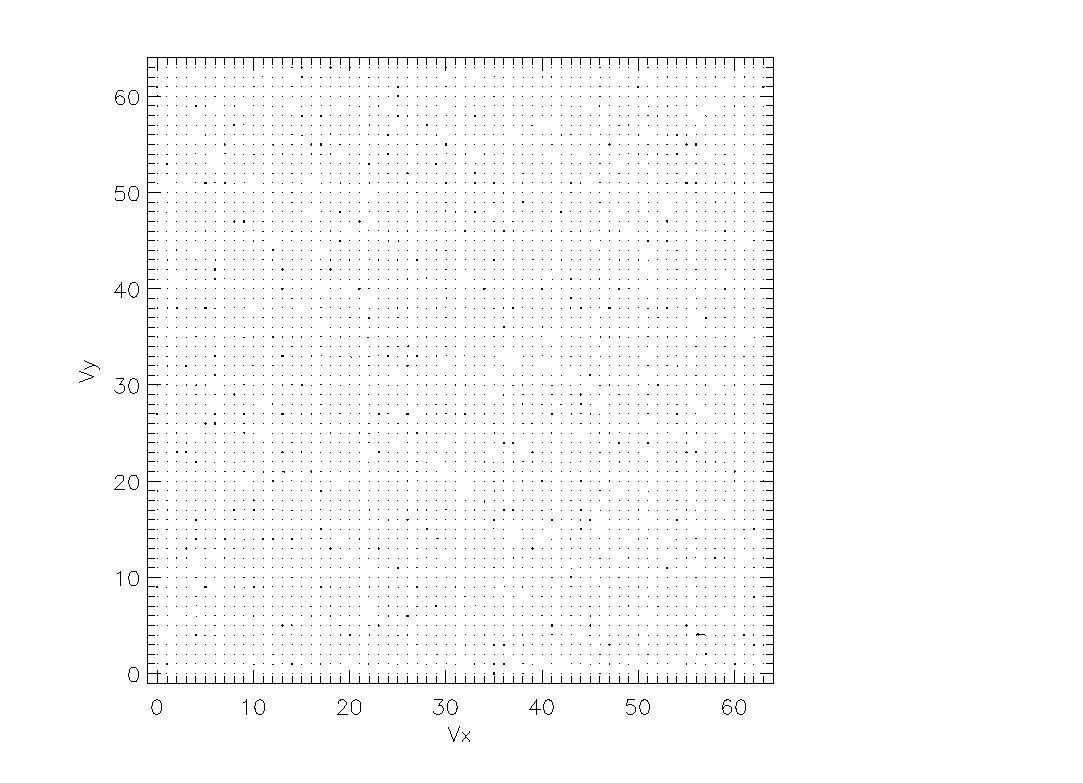
\includegraphics[width=0.49\columnwidth]{./full/wm64/vel/r01000_vel_xy_field}
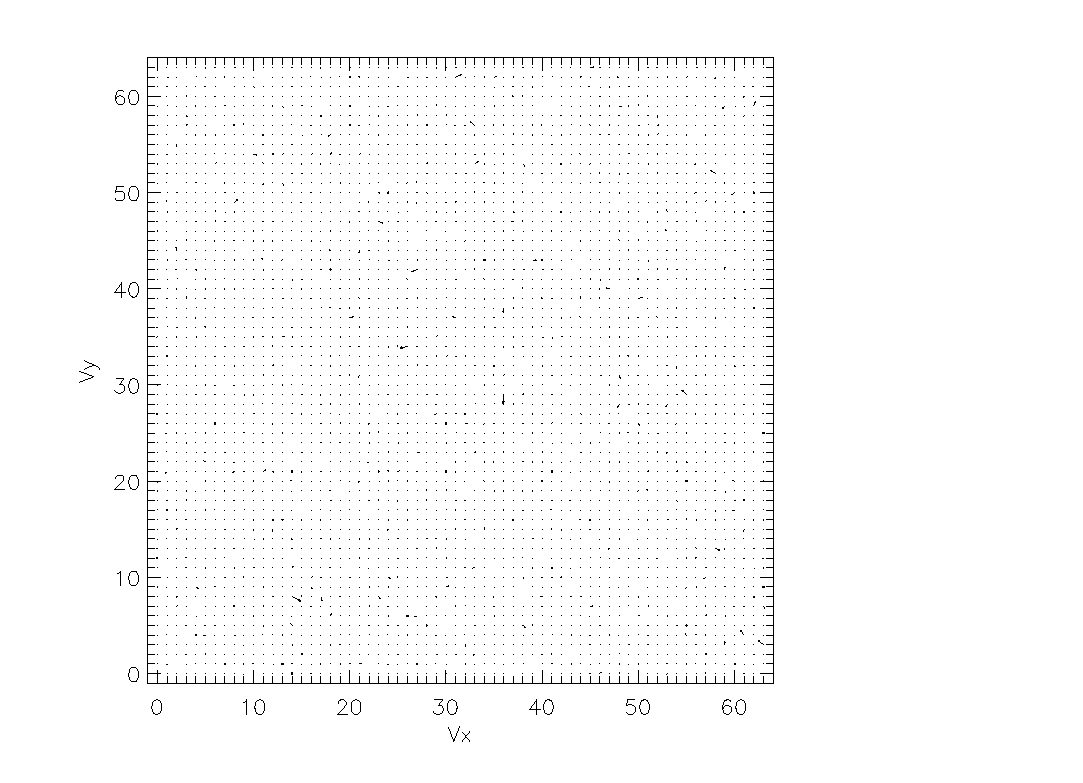
\includegraphics[width=0.49\columnwidth]{./full/wm64/vel/r02000_vel_xy_field}
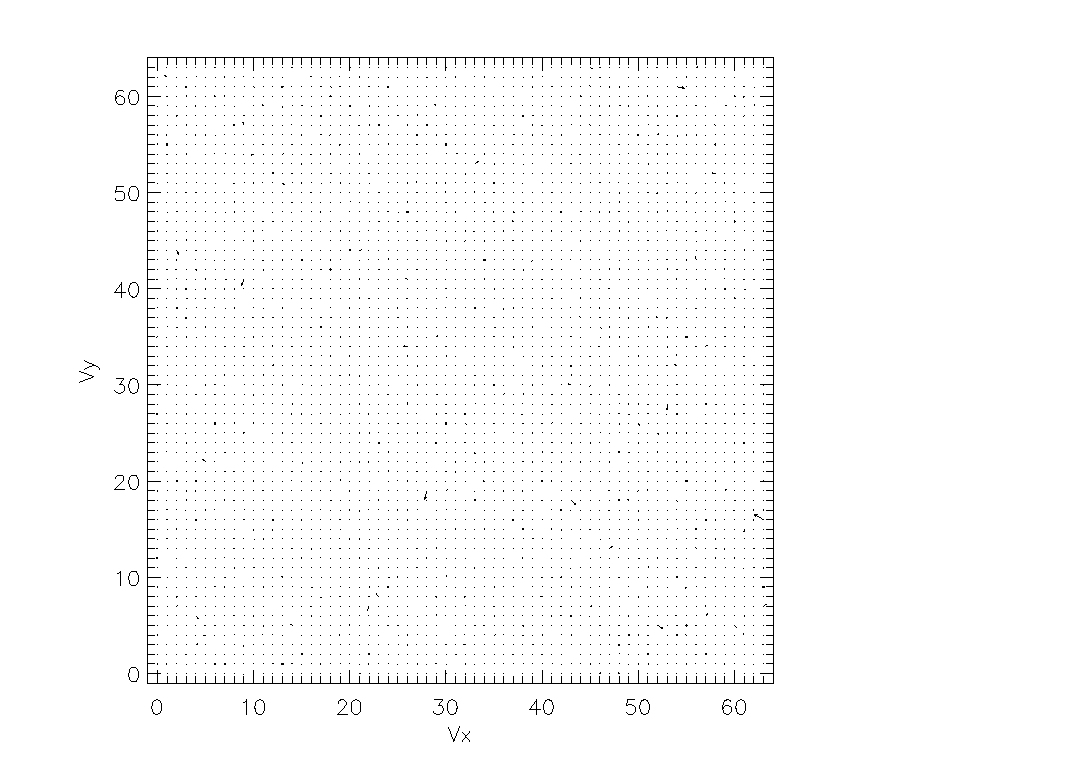
\includegraphics[width=0.49\columnwidth]{./full/wm64/vel/r03000_vel_xy_field}
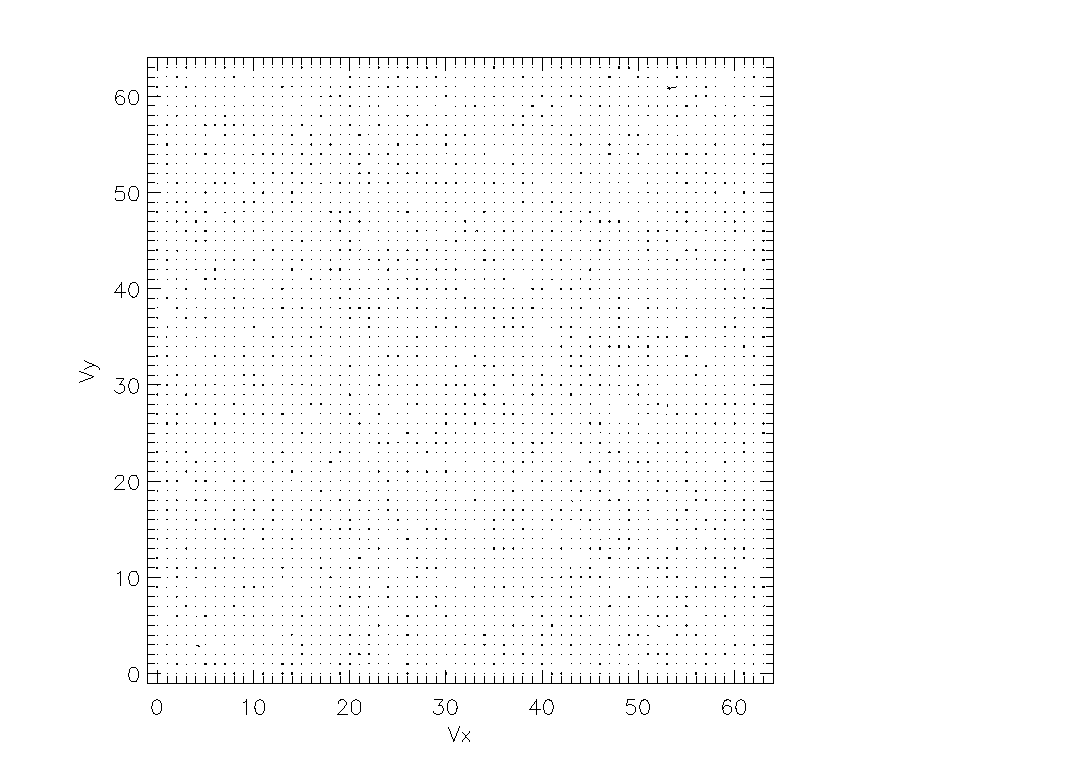
\includegraphics[width=0.49\columnwidth]{./full/wm64/vel/r03500_vel_xy_field}

   \end{center}
\caption{This figure shows quiver plots of the $x,y$ components of velocity from the wave-mechanics code. The velocities are of roughly equal magnitude at early times but this is not true of the later plots. The outputs correspond to the same x,y slice of the data as seen in the previous wave-mechanics plots and at the same times: $t = 0, 200, 1000,$ $2000, 3000, 3500$.}
\label{fig.wmvel}
\end{figure}

\paragraph{Vorticity}
In section \ref{vort} we discussed how to identify possible regions of vorticity, this proved fruitful when analysing the results from the 3D FPA code as sen in section \ref{ch4vort}. In figure \ref{fig.wmvort} the plots show $\mathcal{I}(\psi) \;{\rm vs}\; \mathcal{R}(\psi)$; we suggested that analysing the patterns of these graphs will help to find areas of vorticity and for providing another check of robustness. The first plot shows a ring with an isotropic distribution which implies that both density and velocity are isotropic, this is what we expect from the initial conditions generator supplied by Gadget. It also shows that our construction of the wavefunction is consistent with the initial conditions generator.

The results from the full S-P simulation do not seem to show any signs of vorticity, the wavefunction does not appear to get close enough to zero (min$[\psi_{final} \sim 10]$) to become singular. While the lack of vorticity agrees with the standard theory of cosmology, it is not obvious that singularities are prohibited in our formalism. These singularities were shown in the results of the FPA but there is no good reason for their omission in the results of the full S-P system. Given sufficiently enough time to investigate this phenomena I would try running the simulations for longer to see if they will ever produce a singularity in the wavefunction and hence produce an undefined velocity.

\begin{figure}[htb]
   \begin{center}
     %\leavevmode

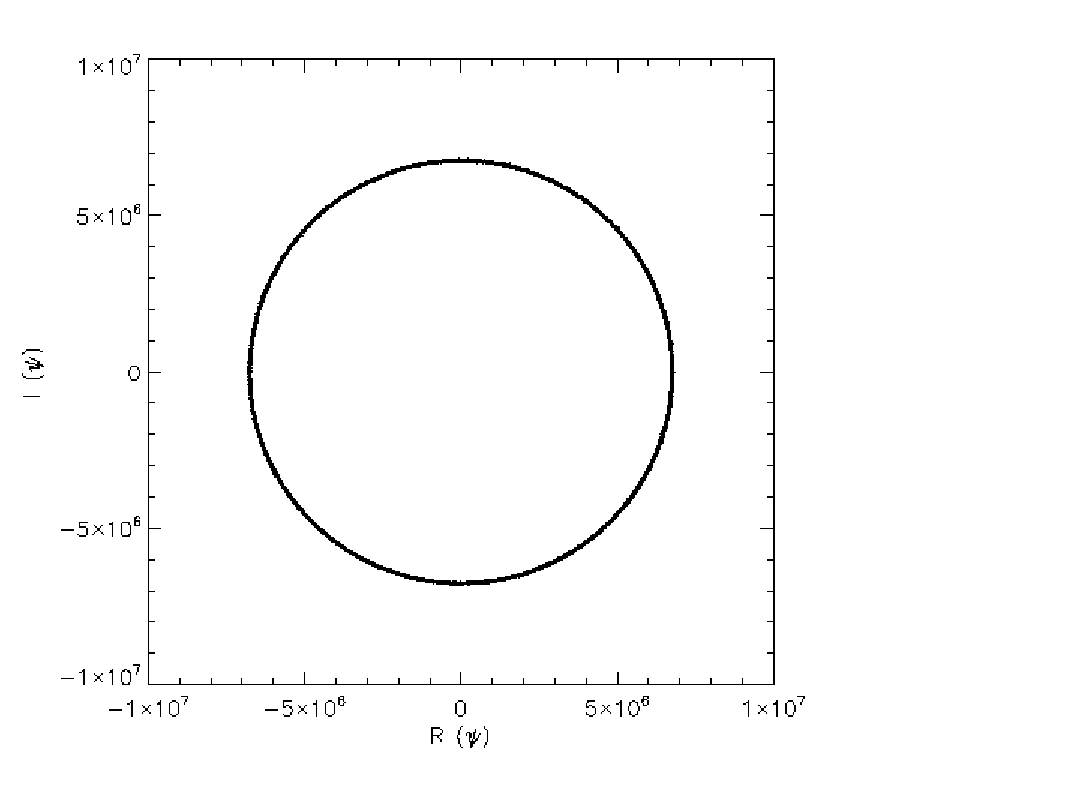
\includegraphics[width=0.49\columnwidth]{./full/wm64/vort/r00000_psi-psi}
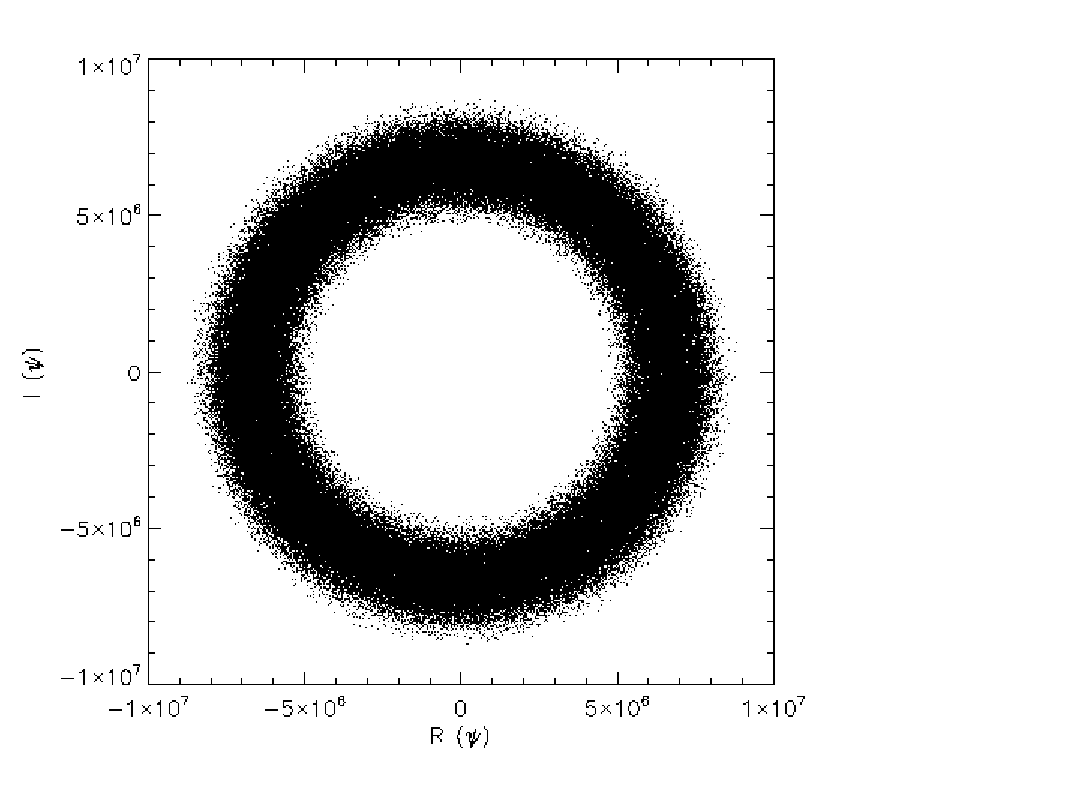
\includegraphics[width=0.49\columnwidth]{./full/wm64/vort/r00200_psi-psi}
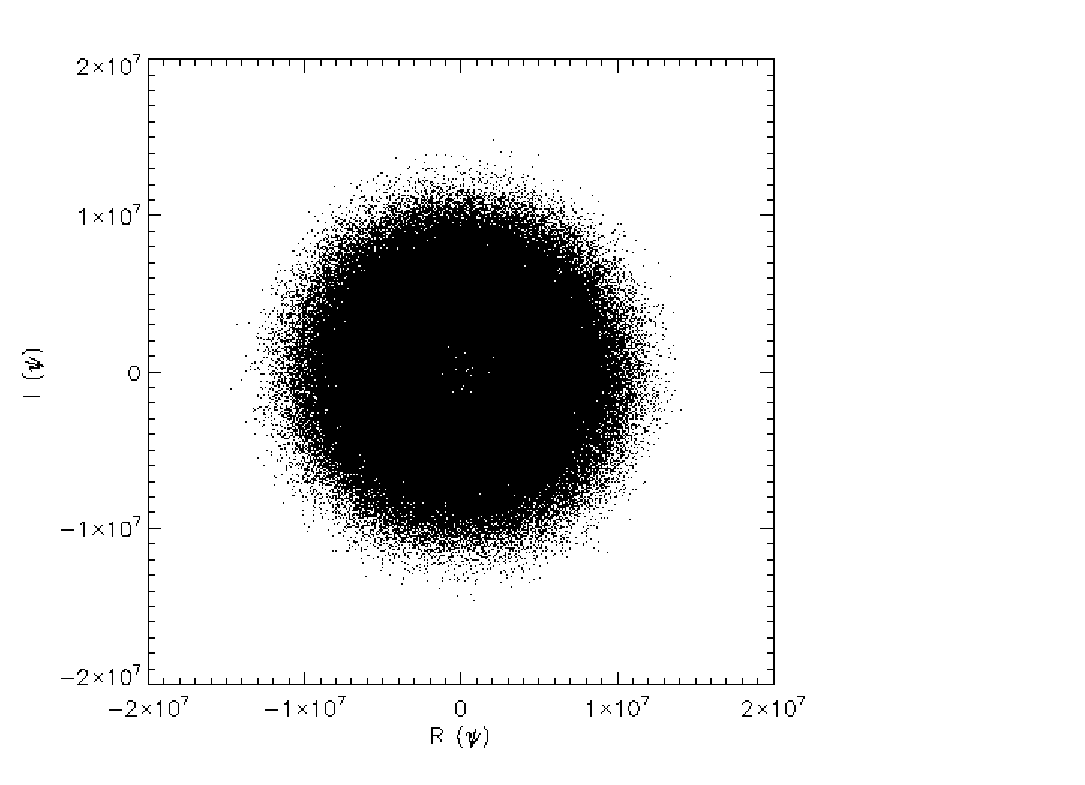
\includegraphics[width=0.49\columnwidth]{./full/wm64/vort/r01000_psi-psi}
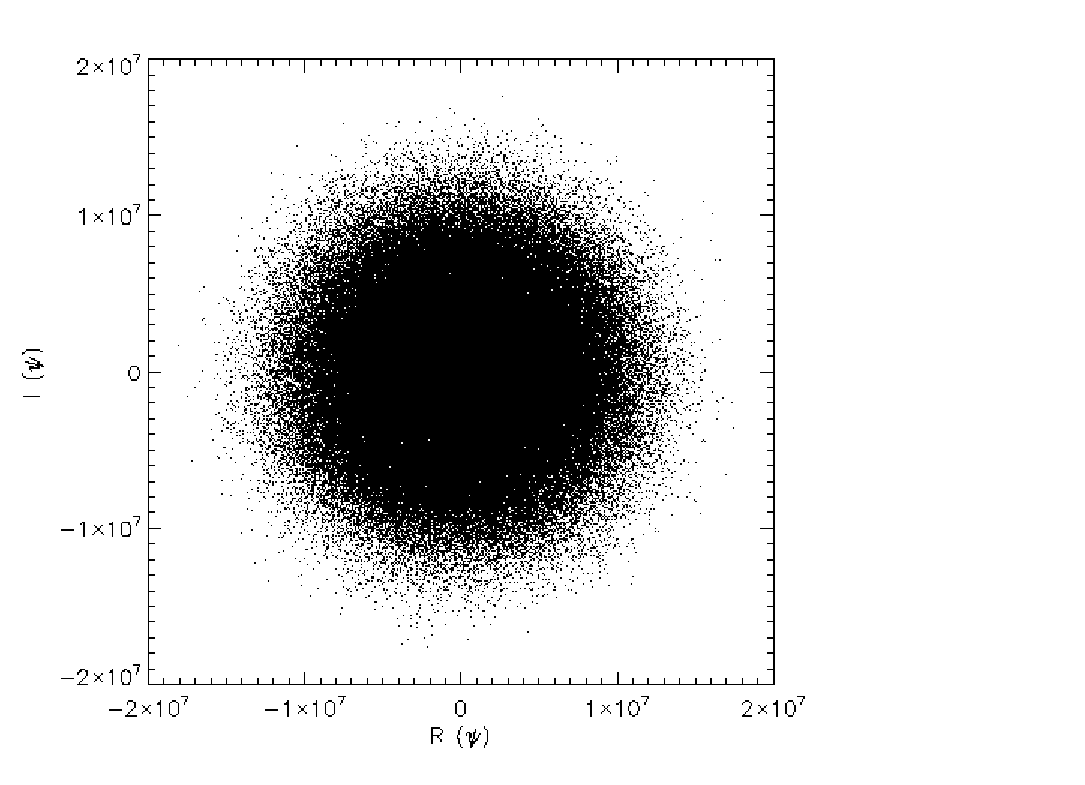
\includegraphics[width=0.49\columnwidth]{./full/wm64/vort/r02000_psi-psi}
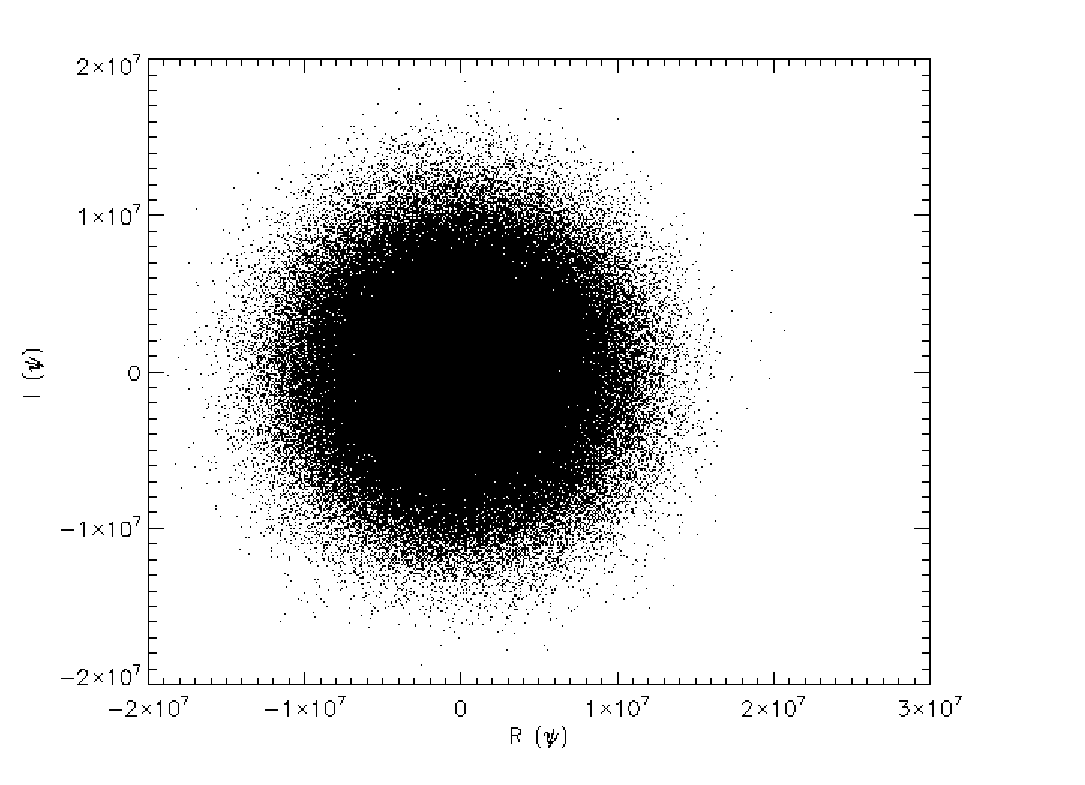
\includegraphics[width=0.49\columnwidth]{./full/wm64/vort/r03000_psi-psi}
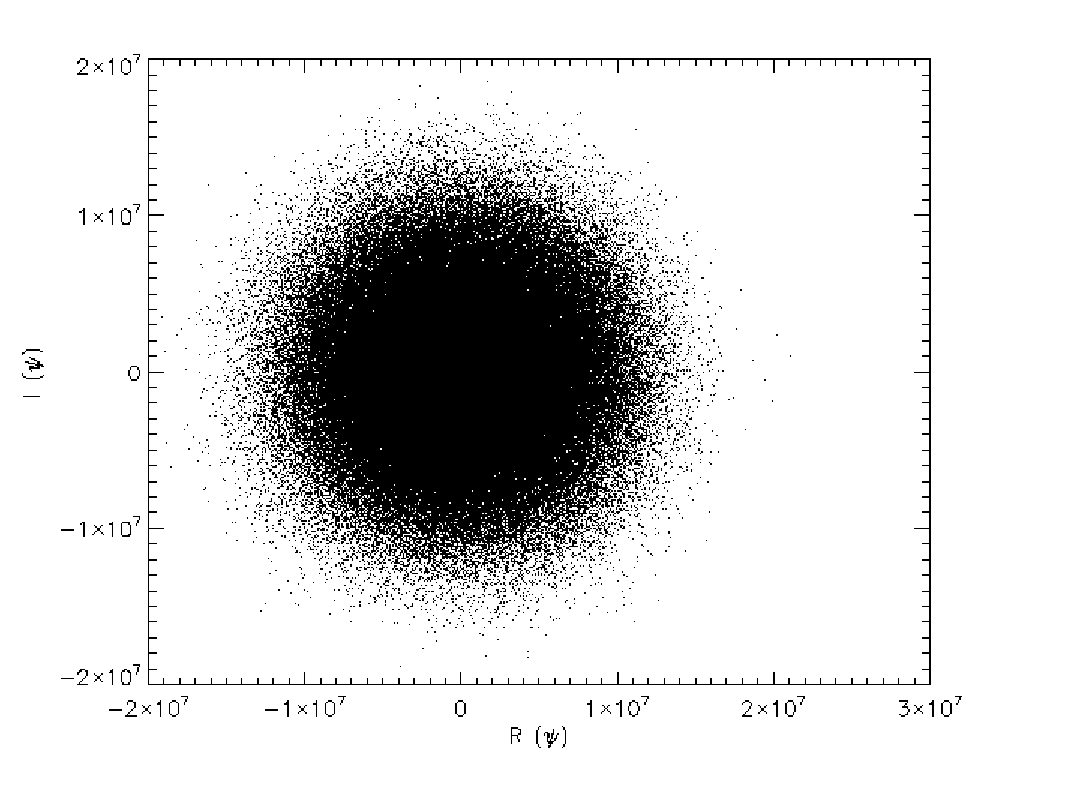
\includegraphics[width=0.49\columnwidth]{./full/wm64/vort/r03500_psi-psi}

   \end{center}
\caption{The plots show $\mathcal{I}(\psi) \;{\rm vs}\; \mathcal{R}(\psi)$. The first plot shows a ring with an isotropic distribution, however the radius is not unity as it was in the FPA, as expected from the initial conditions generator. The smearing out of this ring is indicative that the wavefunction is evolving and hence the over-densities are spread further from the mean. The outputs are at the same times, $t = 0, 200, 1000,$ $2000, 3000, 3500$.}
\label{fig.wmvort}
\end{figure}

\section{Summary}
This chapter has shown how implement a wave-mechanics code for Large Scale Structure that satisfies our five original requirements: 3D coordinates, self-consistent gravity, expanding coordinates, periodic boundaries, mass conserving. The use of the full Schr\"odinger-Poisson equations goes beyond the FPA model of Short. That is to say that we have extended the original paper of Widrow \& Kaiser; which includes a generalization of their Schr\"odinger equation to allow for more cosmological models.

The most similar work to what we have done is the full 3D code from the team in Taiwan. Unfortunately, their publication does not provide enough details to make a full comparison with their technique. There are some open questions about their work that are worth addressing: does it conserve mass and momentum? Does it properly implement periodic boundaries? I suspect that the latter is true because it is a necessary requirement of a cosmological code. I'm less sure of the answer to the former question as they do not address the issue and they may regard it as a less important concern. A key strength of our work is that we have shown that our method conserves mass and momentum.

We have provided a clear roadmap for any reader that would like to create their own wave-mechanics code in order to reproduce our results or to be used for their own purposes. All the necessary mathematics has been provided and clear explanations have elucidated why each piece of the code is necessary and how these pieces fit together. It is clear from the works of Watanabe that the Suzuki splitting operators should be used for any simulation of higher dimension than one. Fortunately, they can be implemented with the Goldberg scheme as suggested by Widrow \& Kaiser (essentially the same as Watanabe's approach). Furthermore, we have shown that the use of splitting operators and the Goldberg scheme can be consistently implemented with periodic boundary conditions and coordinate expansion.

We believe that the implementation of periodic boundaries is completely new as previous publications have not mentioned such considerations. As such, we can confidently state that this is the first illustration of such a method. Also new to this thesis is the generalization of Schr\"odinger equation to describe more general cosmological models.

Proof of multi-streaming (described in section \ref{hydro}), or shell crossing, is clearly shown in the results from the 3D code as seen in section \ref{twobody}. The tophat results show the inclusion of gravity and of a simple cosmologically-based scenario. Such results combined with the conservation of key quantities (mass and momentum) suggest that our final results in section \ref{cos_sim} may be correct but require further investigation. That the whole simulation shares a single wavefunction allows for the possibility of interference, despite our intention to suppress these effects it is still possible that interference is present in our final results (given the apparent messiness of our 3D cosmological results).

A key concern to address is why the density outputs from the wave-mechanics code are not closer to that of Gadget. We expect the results from wave-mechanics to differ from Gadget but it appears that the variation in densities and the patterns produced by wave-mechanics are far greater than expected. As shown in Chapter \ref{ch_4}, the densities from wave-mechanics provided reasonable correlation coefficients with the densities from Hydra. Mass is conserved and the distributions are not completely random; they show a clear pattern of evolution that is different from what we expected but not necessarily wrong. Unfortunately we cannot conclude whether our results are completely correct within the wave-mechanics framework. That is to say that we suspect the wave-mechanics framework is robust and can be correctly applied to LSS simulations but we have not been able to prove that beyond all doubts in this thesis. 

The biggest problem of the wave-mechanics code is the off-centre velocity distribution which suggests a net bulk motion. From theory, the net motion of the Universe should be zero (ignoring suggestions that the Universe might be rotating as a whole). The velocity scaling also appears to be wrong and will need to be addressed in future research.

%
%  Conclusion
%
\chapter{Conclusion}
\label{ch_6}
This thesis provides an overview of wave-mechanics as applied to LSS. The interpretation of the Schr\"odinger equation was re-examined in Chapter \ref{ch_3}, previous inconsistencies and misconceptions were explored and resolved to the best of our ability. Our understanding of wave-mechanics as applied to LSS should now be clearer and more concise. The approach in this thesis is purely classical due to the high particle occupation number in each quantum state, so pure quantum mechanics is never present. The quantum nature of dark matter particles is mostly unknown but not thought to be significant. However this does not affect the main outcome of this work.

Chapter \ref{ch_3} made clear the reason for choosing the Schr\"odinger equation, and not a generic wave-equation, for simulating LSS using a wave-mechanical method. The Schr\"odinger equation is an energy equation where the terms can be easily interpreted in a physical manner using well-developed techniques; there is an obvious link between observables and operators; and the wavefunction is a single complex field that provides a simple method of obtaining the density and velocity.

We have shown the correct interpretation of the Schr\"odinger in this context is that of a generic energy equation that describes the evolution of waves but does not necessarily have to describe a quantum system. In a classical system the effective Planck constant is now analogous to the diffusion coefficient of fluid dynamics. In order to describe such a classical system of $N$ particles one must `multiply up' the single-particle Schr\"odinger equation which assumes a high occupation number.

Also included in Chapter \ref{ch_3} is a modern derivation of the fluid equations from the Schr\"odinger equation. This is lacking in previous  literature. In addition to providing a sketch of the derivation we delved further into the interpretation of the equations, building upon a translation of the original publication by Madelung (see Appendix \ref{app_m}), as well as new insights from later literature and further study.

Crucially, we believe that it is important not to confuse the role of the so-called pressure term. It is a term that highlights the difference between a free particle and a fluid. It is not a term that is `added' in by the Schr\"odinger equation; there is no new or added pressure into the system. In fact, the opposite is closer to the truth. The free particle Schr\"odinger equation describes a fluid that has no internal pressure. Short discovered (under the limit of $\hbar \rightarrow 0$) that the term is only important in regions of high-density. This suggests that the subtraction of the pressure term is negligible and hence a free-particle is the same as a fluid in regions of low density. In high density regions it is natural to expect the pressure to dominate the fluid's evolution.

Johnston, considered a different approach from myself and Short and adds in (by hand) the pressure term in her calculations. Thus, the wavefunction that she describes is truly a fluid.

In Chapter \ref{ch_4}, we presented the results of our investigation of the Free Particle Approximation (FPA) model and confirmed the robustness of the results provided by Short. Our tests were based upon the mathematics provided in his thesis but were carried out using entirely independent codes -- thus representing a fully independent test that reinforces the idea that the FPA is a sound approximation scheme. We were able to conclude that the FPA is a fast and efficient method for probing the quasi-linear regime of density perturbations, it proves to be a good match for the Zel'dovich approximation and breaks down at shell crossing as the Zel'dovich method does. Short proved that the FPA is formally equivalent the Zel'dovich approximation with adhesion (in the limit of $\nu \rightarrow 0$).

The 1D and 3D toy models considered in Chapter \ref{ch_4} were a demonstration of a consistent framework. I have shown that the FPA can handle cosmological initial conditions by providing results that are comparable to the widely available $N$-body codes (at least in the quasi-linear regime). The benefit of the FPA is that it runs much faster than all other known methods of simulation. It merely requires a single step of computation due to the symmetry of the equations.

After developing and testing the FPA, I went on to investigate another method of solving the Schr\"odinger equation, colloquially we call it the Cayley method (Chapter \ref{ch_5}) as it involves describing the exponentials via Cayley's approximation. In this approach we no longer assume the trick that was inherent to the FPA, where the effective potential is zero. In the Cayley approach we solved the full system of equations: both the kinetic term and solved Poisson's equation of gravity.

As shown in Chapter \ref{ch_5}, this process is trickier than it may first appear. Under the recommendation of Watanabe's publication we adopted Suzuki splitting operators and also adopted Widrow \& Kaiser's method of re-writing the equations into a simplified form that deals with timesteps as equal steps in $\ln a$. Fortunately, each component works consistently with one another. The simulations prove to be robust and stable. Consequently, the main goals of developing a wave-mechanics code for LSS were achieved. Those goals were: (1) 3D coordinates, (2) self-consistent gravity, (3) expanding coordinates, (4) periodic boundaries, (5) mass conserving (as a bonus it conserves momentum too). In addition this also satisfies the original goals suggested by Widrow \& Kaiser: A model that describes collisionless matter; matter is described as a field, not particles: that is, continuous; function only of space and time (3+1 d); follow multiple streams in phase space (`hot' / dispersive); competitive with $N$-body techniques for computing time. Sabiu's run with Gadget took approximately the same time to complete as my Wave-mechanics code, of the order of a few hours; however, no rigorous speed testing was conducted in this thesis. Both codes were run on different machines so does not represent a fair comparison but I do expect both codes to be a comparable speed. The number of operations required in each case are similar in magnitude.

The last of our goals (mass conserving) is an indicator of the reliability of our results. Not only did we achieve our goals but have done so in a manner that is consistent with the physics. This was only possible by our strict choice of a symplectic integrator such that the norm of the wavefunction is conserved over time. Hence, this choice of integrator is consistent with unitary time evolution in Quantum Mechanics and further hence that it should be less of a surprise that momentum is conserved as well as mass.

Through out this work I have highlighted the similarities between wave-mechanics and $N$-body simulations. The latter was used as a benchmark for speed and accuracy. However, I have shown wave-mechanics provides a different method for simulating Large Scale Structure. It has many benefits but it lacks the maturity and development seen in modern $N$-body codes. It seems fair to assume that if wave-mechanics is developed further and allowed to run on high-performance machines then it should have no difficulty matching and, perhaps, beating equivalent $N$-body codes for speed and accuracy (in terms of density resolution). This is a guess based on the assumption that the wave-mechanics code can be written to have fewer or less expensive operations than an $N$-body code. In terms of resolution, we believe that a continuous density field representation should ultimately lead to better resolution of the density field. We also believe that wave-mechanics should provide a better representation of the Universe (over $N$-body codes) because they describe a continuous density field and suffers less from discretization problems. The allowance of multi-streaming also prevents two-body relaxation that is a critical issue for $N$-body codes, the current solution to that problem is unphysical and is completely avoided in wave-mechanics.

The main problems with the results presented in this thesis were the unexpected, although not necessarily inconsistent, results for density and velocity. The messiness of the evolved density fields is potentially due to interference, this is unique to a wave-mechanics but not something that desire from a classical system. This effect requires further investigation.

The simulations presented were run at a coarse spatial resolution of $64^3$, this was a problem for generating our initial conditions and hence our subsequent results. At higher resolutions the results look better behaved but were prohibitively more expensive to run within the time frame of this thesis. In order to make sense of the lower resolution simulations we smoothed the data using a gaussian filter (essentially a low pass filter that takes out high frequency `noise'). This operation gave data that looked closer to the Gadget data. We would have liked to use the raw, unsmoothed data, for our point of comparison but it did not look consistent with what we first expected.

The histograms of both density and velocity are initially gaussian and this distribution is fairly well maintained for velocity at all times, while the density becomes a skewed gaussian. The under-dense regions in our wave-mechanics results are evacuated quicker than seen in an $N$-body code but the peaks do not seem to collapse as fast, nor do the peaks reach the same height as seen in the results from Gadget. The choice of the $\nu$ parameter influences the dynamics in such a way that it can greatly affect the collapse speed; in some cases, collapse can be completely prevented. Naturally, the lack of evolution would be inconsistent with what we observe in the real Universe.

These issues will require further investigation but it is our belief that they do not rule out wave-mechanics as a viable method for simulating Large Scale Structure. One of the main concerns we have had is the lack of time needed to run high resolution simulations, although we did some very simple tests at $128^3$ our final runs were at $64^3$ resolution. Initially, we incurred problems from running low resolution simulations where collapse was too fast in the initial timesteps. As mentioned in section \ref{cos_sim}, this effect disappeared for simulations at a resolution of $128^3$. The effect also went away whenever we applied gaussian smoothing to our initial density field.

Given the positive results from this work, we now propose future directions and possible extensions to wave-mechanics codes. We would greatly welcome any reader to reproduce the results from this thesis and / or attempt to implement any of the future work.

\section{Future work: extending the full Schr\"odinger-Poisson system}
In this final section I present ideas that expand upon the standard techniques of wave-mechanics as presented in the previous chapters of this thesis. The aim of this section is for me to develop ideas that will help advance wave-mechanics further and show that our method of evolving structure formation is capable of achieving everything that can be done in an $N$-body code. I see my thesis and all previous work as being the first generation of wave-mechanics codes. The next generation of codes will build upon all previous literature so that they are more diverse in what they achieve, while being also robust.

The best $N$-body codes (such as GADGET and RAMSES) have many more features than current wave-mechanical codes presented hitherto. A short list of features that I believe are desirable for the next generation of wave-mechanics codes, and are already prominent in the best $N$-body codes, are: 
(1) multiple particle/fluid species, (2) adaptive mesh refinement, (3) parallelization.

In this chapter I will review each item in the above list and expand upon how one might implement these features into a wave-mechanics code. Fortunately these ideas have already been explored to some extent in previous publications; however, they are yet to be featured in a full cosmological wave-mechanics code. Johnston \citep{bib_rj} has already written a code that models two species of fluid and Watanabe \citep{bib_wat} has provided many ideas that can be included in a next generation of wave-mechanical LSS codes: such as a possible method for implementing mesh refinement and parallelization. The following ideas are presented in the remainder of this thesis:

\begin{itemize}
\item Multiple fluids
\item The splitting operator approach to including more physics (such as pressure)
\item Periodic boundaries via adhesive operators
\item Mesh refinement
\item Parallelization
\item Including vorticity and spin
\end{itemize}

\noindent The last bullet point will be presented in the next chapter, they are less conventional and hence far more speculative. They are effects that are not currently accounted for in standard LSS simulations. These ideas are the inclusion of gravitomagnetism and spinning objects into a wave-mechanics code. Both ideas might allow wave-mechanics codes to potentially probe beyond the standard model of cosmology.


\subsection{Multiple fluids}
The idea of a multiple particle-species is not new to $N$-body codes. Special variants \citep{bib_hmpc1} of the Hydra code \citep{bib_hmpc} allows for Baryons as well as CDM particles to be present, these codes have been written to account for gas dynamics where the Baryons will behave as dispersive particles with an associated temperature.

Johnston has shown how to include another fluid of the same mass into a Schr\"odinger code. The two species have separate wavefunctions with separate Schr\"odinger equations except that they have a common gravitational potential. In principle this is easy to extend to $N$ species of particles (or fluids). The initial mass of each fluid is allowed to be different, this will be expressed by the fact that the total mass of the wavefunction for each species will be different. It would also be possible to alter the value of $\nu = \hbar/m$ for each species, hence account for different dispersion properties.

I believe that the splitting operators presented in this thesis provide a natural way of adding new particle species in a modular way. Here I will briefly recapitulate how this method evolves the wavefunction:

\begin{equation}
\psi(x, t+dt) = e^{-i (K+V) dt} \psi(x, t) = e^{-i K dt/2}e^{-i V dt}e^{-i K dt/2} \psi(x, t)
\end{equation}

\noindent We have chosen to split the kinetic energy operator such that one half timestep is performed before and then after the potential energy operator. I envisage performing each half-step kinetic operator sequentially for 1 to $N$ (the number of species / fluids) then performing the calculation of a common gravitational potential. Here is an overview of how I expect the evolution part of the algorithm to look:

\begin{enumerate}
\item $\psi_{1 \ldots N}(t + \frac{1}{2} dt) = \hat{K}_{1 \ldots N} \; \psi_{1 \ldots N} (t)$
\item $\psi_{1 \ldots N}(t + \frac{1}{2} dt) = \hat{V}_{1 \ldots N} \; \psi_{1 \ldots N} (t + \frac{1}{2} dt)$
\item $\psi_{1 \ldots N}(t + dt) = \hat{K}_{1 \ldots N} \; \psi_{1 \ldots N} (t + \frac{1}{2} dt)$
\end{enumerate}

\noindent Here I denote the kinetic energy operator by $\hat{K}$ and the potential energy operator by $\hat{V}$. The subscripts ${1 \ldots N}$ denote the different particle species.

The operator $\hat{K}$ above is stated generically so the kinetic operator for each species could have a different value of $\nu$. It would also be possible to modify the kinetic energy operator of each species too, although there are limits to how far the operator can be modified: for example, the addition of any term that does not commute with the kinetic energy is very likely to break the energy conservation of the code.

To properly account for additional physics one would need to split the operators (in a nested fashion) as Suzuki suggests. For example it should be possible to include Baryons having internal interactions.

\subsection{Including additional physics}
\label{addphys}
If I was to add pressure into my code (as Johnston did) I think I would need to include it as a separate split-operator. I don't believe that it would be entirely correct to modify the kinetic energy operator to account for pressure, for example simply writing $\hat{\tilde{K}} = \hat{K} + \hat{P}$. The evolution would then be written as (this is in short hand form, I omit $i, \; {\rm dt},$ etc in the exponential):

\begin{equation}
\exp(\hat{\tilde{K}})\psi(t) = \exp(\hat{K} + \hat{P}) \psi(t)
\end{equation}

\noindent To properly account for pressure in a robust manner in the Cayley method then one would need to separate the operators in a way that is consistent with Suzuki's method of decomposition. The full decomposition of the Hamiltonian (including all 3 terms: kinetic, potential and pressure) is:

\begin{equation}
\exp(\hat{K}+\hat{V}+\hat{P})\psi(t)\rightarrow  \exp(\frac{1}{2}\hat{K})\exp(\frac{1}{2}\hat{P})\exp(\hat{V}) \exp(\frac{1}{2}\hat{P})\exp(\frac{1}{2}\hat{K}) \psi(t)
\end{equation}

\noindent I believe this would be true for the inclusion of any number of operators, provided they are split up in the manner that Suzuki suggests. In a second paper from Watanabe \& Tsukada \citep{bib_wat2}, they show how to use the Suzuki splitting operators to include a magnetic potential when simulating the dynamics of an electron in a magnetic field.

\subsection{Periodic boundaries via adhesive operators}
As mentioned in section \ref{per_bound}, Watanabe \citep{bib_wat} suggested a method for implementing periodic boundary conditions that he coined `adhesive operators' (not to be confused with the Zel'dovich adhesion model). These `operators' connected one boundary to another (connects the boundaries like an adhesive) such that waves that exited on the left-hand-side of the system and would reappear on the right-hand-side. I believe that if these operators can be successfully implemented in a cosmological wave-mechanics code then it would save on computing time as my method (section \ref{per_bound}) involves a double iteration of each recursion relation can be avoided. As already mentioned, I made a brief attempt to implement periodic boundaries in this way but it did not conserve mass. Any possible method that can cut computing time but preserve unitarity would be worth investigating.

Watanabe's idea is simple and elegant; the mathematics is relatively straight forward but it seems that not enough details are provided in the publication of Watanabe to ensure perfect implementation. Also, as previously mentioned, it is not obvious that such operators would overcome the inherent problem of the recursion relations for the auxiliary functions ($e$ and $f$).

Watanabe's adhesive operators are ubiquitous, he uses them for the implementation of periodic boundaries, mesh refinement and parallelization. Hence, we believe that such a method if it can be independently proven to work would yield a powerful method for improving speed, accuracy and size of simulations.

Here is a brief sketch of Watanabe's idea. He notes that in a crystal the wavefunction can be taken as periodic, that is to say that some region far from the real boundaries of the crystal will look like a repeating unit of a larger lattice. Hence, the extent of the lattice is pseudo-infinite. This is the same type of argument that is made for using periodic boundary conditions in cosmological simulations. The wavefunction obeys the periodic relation:

\begin{equation}
\psi({\bf r} + {\bf R},t )= \psi({\bf r},t)e^{(i\phi)}, \;\;\; \phi = {\bf k}.{\bf R}
\end{equation}

\noindent ${\bf k}$ is the Bloch wavenumber and ${\bf R}$ is the length of the lattice (although Watanabe calls this the unit vector, implying it should be the spacing between gridpoints). Bloch's theorem requires the modulus of the exponential to be one, hence the modulus of the wavefunction is also preserved. This is necessary for a smooth transition at the boundary and for unitary time evolution. For code implementation, these modifications appear in the $\Omega$ function of Goldberg. Recall that when using splitting operators the potential $V$ is separate from the kinetic operator $K$ and hence taken out of the $\Omega$ function as seen in Goldberg. Hence the adhesive operators are a modification to the kinetic energy operator. Copying Watanabe's notation we write the matrices for the time evolution in the following manner ($V$ is omitted):

%\[
\begin{eqnarray}
\left(\begin{array}{cccccc}
A & -1 & 0  & 0 &\ldots & e^{+i\phi} \\
-1 & A & -1 & 0 &\ldots & 0 \\
0 & -1 & A  & -1&\ldots & 0 \\
\vdots & & & & & \vdots \\
e^{-i\phi}& 0 & \ldots & 0 & -1 & A
\end{array}\right)
\left(\begin{array}{c}
\psi(0,t + dt) \\
\psi(1,t + dt) \\
\psi(2,t + dt) \\
\vdots \\
\psi(L-1,t + dt) \\
\end{array}\right) \\
=
\left(\begin{array}{cccccc}
B & -1 & 0  & 0 &\ldots & e^{+i\phi} \\
-1 & B & -1 & 0 &\ldots & 0 \\
0 & -1 & B  & -1&\ldots & 0 \\
\vdots & & & & & \vdots \\
e^{-i\phi}& 0 & \ldots & 0 & -1 & B
\end{array}\right)
\left(\begin{array}{c}
\psi(0,t) \\
\psi(1,t) \\
\psi(2,t) \\
\vdots \\
\psi(L-1,t) \\
\end{array}\right)
\end{eqnarray}
%\]

\noindent the definitions of $A$ and $B$ are not necessary for understanding the method. In the simplest case $A$ and $B$ take the expected form as you would expect from the kinetic energy matrices as they appear in section \ref{onedim}. Here we use $L$ to denote the length of the lattice, so $L-1$ is the last element of the array.

As Watanabe notes, the addition of these off-diagonal elements should prevent the matrices finding an efficient solution. The usual methods of inversion work well for diagonal, or band-diagonal, matrices but not non-diagonal matrices. However, the trick is to note that the first line and the last line of the operator matrices can be solved independently from the rest of the matrix: $\partial^2_x = \partial^2_{x-td} + \partial^2_{x-ad}$. The kinetic energy can be written as the matrix addition of the tridiagonal contribution $\partial^2_{x-td}$ and the off-diagonal terms (the adhesive operator) $\partial^2_{x-ad}$.

An alternative method for periodic boundaries would be the use of Fourier transforms as they are inherently periodic. However, our attempts to implement the kinetic energy operator via an FFT method have been unsuccessful.

\subsection{Mesh refinement}
Mesh refinement is a method of improving the code's efficiency. Regions that are known to grow into large densities can be pre-binned before the simulation starts. That is, the mesh can be of a finer resolution in areas of higher density. Alternatively, a more computationally expensive way would be to allow the computer to determine how to bin the data on the fly using so-called Adaptive Mesh Refinement (AMR). Static mesh refinement requires the user to know where the high density regions form and would require a lot of effort for each new simulation.

AMR is not a new idea, nor are ideas of adaptive quadrature, but such an idea is missing in the current wave-mechanics of LSS literature.
Watanabe (\citeyear{bib_wat}) has shown how to include mesh refinement in a Schr\"odinger solver. Mesh refinement is easily achievable for the kinetic energy operator by use of Watanabe's adhesive operators. The potential energy calculation requires separate consideration. Such an idea is particularly attractive for LSS simulations and should perhaps be one of the first avenues for future wave-mechanics research. It can provide increased spatial resolution in the areas that need it most.

For mesh refinement, Watanabe decomposes the kinetic energy operator into two parts: one part that is easy to solve (the diagonal) and the part that requires a separate calculation in the manner of the adhesive operator. The main difference between the refined calculation and the non-refined is that the kinetic energy operator may require more than 3 gridpoints for calculation and that the weightings for each gridpoint are not necessarily the usual -1, +2, -1 as seen for the central difference method. The weightings can be fractional, as in equations (32 - 34) of Watanabe (\citeyear{bib_wat}).

\subsection{Parallelization}
Another key development for increasing the size of simulations is to develop a way of parallelizing the wave-mechanics code. Some parallel Schr\"odinger solvers \citep{bib_yee, bib_schn, bib_str} exist but their method is different from the Goldberg/Cayley scheme as used in this thesis. Furthermore, it is not entirely obvious how reliable these codes are. The recursion relations are inherently difficult, if not impossible, to put into a parallel code. Ideally, the wavefunction can be split up into independent regions and then evolved by $dt$. The regions would then be reconciled with the whole simulation at the end of each time step.

For parallelization Watanabe suggests the use of his adhesive operators again: they can connect two regions, or two boundaries, with ease. Each region is calculated independently and then matched at the boundary.

Without the adhesive operators, one would need to run a single set of recursion relations over multiple processors. Each processor would rely upon the processor before it in the chain. This is much slower than if each processor can work independently then pass data at the end of each calculation set. This becomes very expensive when periodic boundaries are required.

In the absence of periodic boundaries, where only one recursion is necessary, the recursion relations can be staggered: while the second processor continues the recursion relation for $e$, processor one could start the recursion relation for $f$. When periodic boundaries are implemented this inevitably means that the first processor is idle while the next second processor continues with the recursion. This is necessary as the second iteration of each recursion relation requires the last value in the sequence (comes from the last processor) before starting again.

The lack of a clear parallelization scheme will inhibit progress in wave-mechanics. Future research into this area may have to choose a different Schr\"odinger solver if such a solver is able to be parallelized while being reliable.



%
%%
%%%
%%%%
\chapter{Epilogue: Vorticity and spin}
\label{ch_7}
This chapter is not part of the work of this thesis. The aim of this chapter is to demonstrate that wave-mechanics is a method of simulation that may be naturally suited to including vorticity and spin. In section \ref{vort} I pointed out that singularities in the wavefunction ($\psi = (0,0), \;\psi\in\mathbb{C}$) may indicate the centrepoint of a vortex. In a standard $N$-body or wave-mechanical simulation we do not expect to see any vorticity, as previously mentioned, due to Kelvin's circulation theorem. This rules out vortical motion at small distance scales. We expect the circulation theorem to hold as gravity is a conservative force and can be expressed as the derivative of a scalar potential, hence the curl of the force is identically zero: $\nabla\times F_g = \nabla\times\nabla\phi_g \equiv 0$.

When the wavefunction is singular ($\psi = (0,0), \;\psi\in\mathbb{C}$) then the velocity at such a point is undefined (see equation \ref{eqn_svel}). It could be possible that such a region is not a vortex at all but is rather a region of numerical unreliability; however, there is an interesting similarity between this type of singularity in the wavefunction and a vortex: the velocity vector at the centre of a vortex is also undefined.

In Short's thesis he provided the caveat that the circulation theorem only holds before shell crossing \citep{bib_short}; therefore, the existence of small scale vorticity does not contradict Kelvin's theorem as their existence would only occur after or in regions of shell crossing. Kelvin's theorem does not forbid large scale rotation either, for example such phenomena are clearly visible in the published video of the Millennium Simulation \citep{bib_mil}. Given that singularities and possible sources of vorticity exist in our wave-mechanics data (for example, see \ref{fig.psi_psi} \& \ref{fig.vort}), then to what extent do we expect vorticity to be relevant in the dynamics of an arbitrary astrophysical system?

We know that vorticity occurs naturally in electromagnetism and that regions with a strong magnetic field should display vortical or helical motion, such as charged particles following the magnetic field in a solar flare. However, we don't expect to see vorticity at cosmological scales. In cosmological simulations the initial angular momentum is set to zero which is observationally motivated as suggested in Chapter \ref{ch_1}; furthermore, we expect the vorticity to be zero in the Universe now as it is related to the decaying mode of density perturbations (as mentioned in section \ref{lingrow}). Despite the fact that this thesis has focussed upon applying wave-mechanics to large scale structure it should be possible to simulate systems of smaller scales such as individual galaxies or proto-planetary disks where vorticity may be more relevant.

In the conclusion to Short's thesis \citep{bib_short} he suggests that the wave-mechanical method might be able to model the rotation of CDM haloes, he suggests that this could potentially be done by incorporating spin in a similar way that the Pauli equation does. In this chapter we present two bold ideas that can (1) be used to probe regions of vorticity and (2) investigate the spin of self-gravitating masses. The latter deals with the intrinsic spinning motion of a single object (which could be infinitesimal in size), while the former deals with circular or spinning motion at the scale of a few particles.

In this chapter I will show, particularly in section \ref{spinobj}, that adding spin is not necessarily the same as adding vorticity. It should be possible to include spin effects in a system that has a Newtonian gravitational potential. If we combine both spin and vorticity then we could account for spin-orbit coupling; admittedly, this is likely to be a more profound effect in simulations of highly dense or high spinning systems such as AGN or neutron star / black hole binaries but it could have interesting and unforeseen consequences in a cosmological simulation.

\section{Vorticity}
In order to properly handle vorticity we will need to modify our equation for the force of gravity in such a way that the curl of the force is no longer forbidden. We could we propose a phenomenological fix to the problem of vorticity by invoking a gravitational vector-potential, let's call it $V_c$ and note that the curl of the gravitational force is now: $\nabla\times F_g = \nabla\times(\nabla\phi_g + V_c) \not\equiv 0$. This expression is no longer identically equal to zero; it is possible that the new potential is negligible and hence the curl of force is very close to zero anyway.

We wish to add this extra complication as an extra degree of freedom such that it may yield additional physical effects. We are primarily interested in setting this vector potential to zero initially but then watching the evolution of our system to see if the potential is non-zero by the end of the simulation. As noted we have seen rotation on large scales in the Millennium Simulation \citep{bib_mil} but by providing this additional freedom we might see rotation, and hence vorticity, on smaller scales than we currently do without radically increasing the resolution of the simulation. This could provide a more reliable way of simulating how gravity can `torque up' an extended body such as a galaxy or a group of bodies like our Local Group.

It is not obvious if such torque effects would be significant for LSS simulations, torques should be present without the existence of vortices. It is possible to study torque and angular momentum in current $N$-body simulations without the inclusion of a vector potential; however the existence of a vector potential would naturally allow for torquing force (one that acts tangentially to the ordinary force of gravity).

The effects of torque upon galaxies have been considered in a publication by Gonz\'alez-S\'anchez \& Teodoro \citep{bib_gonz}. These authors considered the torque upon galaxies in clusters that is generated from the gravitational force and a dynamical force of friction. They used this to study the possible origin of small-scale alignment effects of galaxies within clusters. Their motivation for torque is more like the second idea proposed in this chapter, where the galaxies are dipole-like masses (that is to say that they are not point particles). The suggestion for this section is to study the inclusion of a gravitational vector-potential but the particles (in an $N$-body code) are still point particles.

If a region of vorticity is identified in an LSS simulation then finding the centre of the vortex could be a possible method of identifying spiral galaxies or a small group of galaxies. Such a method is probably unable to identify elliptical galaxies. Researchers in the field of $N$-body simulations use the Halo Model \citep{bib_halo} to populate their density field (actually a CDM density field) with galaxies. This model is only appropriate to particle simulations and could not be translated into a wave-mechanical perspective as easily. Hence, wave-mechanics requires an alternative method of populating the density field with galaxies; therefore, identifying vortical regions with non-zero mass is one possibility.

I provide the caveat that a singular region where the wavefunction is zero requires the density to be zero as well. The original suggestion for finding vorticity was to look at gridpoints where the wavefunction is zero; however, for the velocity to be undefined it requires only the imaginary part of the wavefunction to zero. It should be possible to identify regions where the density $\rho = \psi^*\psi$ is non-zero but the velocity is undefined; the wavefunction would take a form $\psi = (a,b)$ where $\; a \neq 0,\; b = 0;\; a, b\in\mathbb{R}; \;\psi\in\mathbb{C}$.

\subsection{Gravitoelectromagnetism}
\label{GEM}
In the previous few paragraphs we suggested that including vorticity could be done using a vector-potential. Clearly, this potential does not need to be gravity but could be some other force. It could perhaps be the magnetic field from electromagnetism; a wave-mechanics simulation that includes Newtonian gravity and a magnetic field might be useful in simulating, for example, neutron star binaries where the magnetic field is non-negligible. Otherwise the stipulation of a gravitational vector-potential will seem like a phenomenological proposition.

From searching into previous literature on vector-potentials in gravity we discovered that the idea called Gravitoelectromagnetism (GEM)  \citep{bib_gravito} provides such a potential (it provides a gravitational vector potential). GEM is attractive on two counts: (1) it already provides a gravitational vector-potential and (2) the idea is well established and relies upon equations that are analogous to Maxwell's equations. On the latter point, the Maxwell equations have already been shown to fit into the Schr\"odinger equation and Watanabe \citep{bib_wat2} has also a suggested a way for handing the vector potential using the Cayley method.

GEM is formally analogous to the Maxwell equations, the vector-potential $A$ is no longer associated with electromagnetism but is instead a gravitational vector-potential (denoted $A_g$). This potential can be called the gravitomagnetic potential but has nothing to do with classical magnetism. Under certain conditions it can be shown that GEM is a valid approximation to Einstein's field equations  \citep{bib_gravito}.

\vspace*{1cm}
\begin{center}
\begin{tabular}{|r|l|}
  \hline
  GEM equations & Maxwell's equations \\ \hline
$\nabla \cdot \mathbf{E}_\text{g} = -4 \pi G \rho_\text{g}$  & $\nabla \cdot \mathbf{E} =  \frac{\rho}{\epsilon_0}$ \\
$\nabla \cdot \mathbf{B}_\text{g} = 0$ & $\nabla \cdot \mathbf{B} = 0$ \\
$\nabla\times\mathbf{E}_\text{g}= -\frac{\partial\mathbf{B}_\text{g}}{\partial t}$& $\nabla\times\mathbf{E} = -\frac{\partial\mathbf{B}}{\partial t}$\\
$\nabla \times \mathbf{B}_\text{g} = -\frac{4 \pi G}{c^2} \mathbf{J}_\text{g} + \frac{1}{c^2} \frac{\partial \mathbf{E}_\text{g}} {\partial t}$ & $\nabla \times \mathbf{B} = \frac{1}{\epsilon_0 c^2} \mathbf{J} + \frac{1}{c^2} \frac{\partial \mathbf{E}} {\partial t}$ \\
  \hline
\end{tabular}
\end{center}
\vspace*{1cm}

\noindent On the right hand side are the standard Maxwell equations with the usual meanings from electromagnetism. On the left we have new quantities. Here, $E_g$ is the gravitoelectric field, or the field from static gravity. It is directly comparable to Poisson's equation: $\nabla^2 \Phi_g = -4 \pi G \rho_\text{g}$. Likewise the new field $B_g$ is the gravitomagnetic field; $\rho_g$ is simply the mass density as it appeared earlier in this thesis and has a corresponding mass-current density which is denoted by $J_g$. This latter quantity, $J_g$, is essentially the same one found earlier in this thesis although it will account for some relativistic effects given the context.

\paragraph{Vorticity}
From a theoretical point of view it is easy to imagine vorticity being generated by a force analogous to the magnetic field. The magnetic field in electromagnetism merely bends trajectories of particles rather than increasing their speed. Therefore it is natural to construct a Lorentz force for GEM:

\begin{equation}
\mathbf{F}_\text{g} = m \left( \mathbf{E}_\text{g} + \mathbf{v} \times 2 \mathbf{B}_\text{g} \right) 
\end{equation}

\noindent The gravitoelectric field $E_g = \nabla\phi_g$ will provide the usual curl-free Newtonian force of gravity, whenever the gravitomagnetic field $B_g$ is zero then the usual Newtonian force of gravity is recovered. The gravitomagnetic force will act perpendicular to the direction of velocity, which would act to bend the trajectory of the mass it acts upon. It is clear that this field is not necessarily curl free, hence the generation of vorticity is not formally forbidden.

Any system that obeys the GEM equations can be described using a Schr\"odinger-like equation, as has been shown for the dynamics of an electron in a magnetic field \citep{bib_wat2}.

\paragraph{Schr\"odinger equation}
Watanabe's publication \citep{bib_wat2} that describes electrons in a magnetic field presents the following Schr\"odinger equation:

\begin{equation}
i\hbar\frac{\partial}{\partial t}\psi(\underline{x},t) =-\frac{\hbar^2}{2m}\left(\nabla^2-\frac{ie}{\hbar}\mathbf{A}\right)^2 \psi(\underline{x},t)
\end{equation}

\noindent For simplicity, this equation omits the usual scalar potential $V$. In the GEM case then the electric charge $e$ would be replaced by the gravitational ``charge'' (mass) $m$. As for electromagnetism, there is the expected relation that $B_g = \nabla \times A_g$. The EM version of this equation is consistent with the EM Maxwell equations; therefore, by construction, the gravitational Maxwell equations will be consistent with the GEM Schr\"odinger equation by making the appropriate replacements (such as $A \rightarrow A_g$).

Watanabe only presented a 1D magnetic force but it is straight forward to generalize this to a 3D (gravito-)magnetic force. As expected he decomposes the evolution of this Schr\"odinger equation using splitting operators. He notes ``the magnetic field just changes the phase of the wavefunction, so it is very easy to compute.''

\subsubsection{Test of Gravitomagnetism}
We expect the gravitomagnetic force to provide a torque, or twisting force, to the masses in our simulations. In the previous section we mentioned that simulations of Large Scale Structure already display regions under going rotational motion, hence they have non-zero angular momentum. We therefore expect the gravitomagnetic field to be non-zero in existing simulations; naturally, the effect is not included in the equations of motion but the field $B_g$ is proportional to the angular momentum, $L$, of the system ($L\neq 0 \Rightarrow B_g \neq 0$).

In an LSS simulation we expect the the effect would be small even if the field was included in the equations of motion; therefore, the effect is likely to be smaller in a simulation that does not have the field $B_g$ in its equations of motion. We performed a test of the latter to see if we could find a non-zero $B_g$ field from the data of our Hydra simulations (as seen in Chapter \ref{ch_4}. We constructed a code that would take an output from Hydra (position and velocities of all particles) and then calculate the field $B_g$ which is defined as follows:

\begin{equation}
\mathbf{B}_\text{g} = \frac{G }{2 c^2} \frac{\mathbf{L} - 3(\mathbf{L} \cdot \mathbf{r}/r) \mathbf{r}/r}{r^3}
\end{equation}

\noindent here $\mathbf{L}$ is the angular momentum of a particle in the simulation and $\mathbf{r}$ is the position of the particle (relative to the centre of mass). The angular momentum is defined as:

\begin{equation}
\mathbf{L} = \int \rho (\mathbf{v} \times \mathbf{r}) dV = \sum m (\mathbf{v} \times \mathbf{r})
\end{equation}

\noindent here $\mathbf{v}$ is the velocity of a particle relative to the centre of mass, $\rho$ is the density and forms the definition of a continuous angular momentum field however it is sufficient to work with discrete masses using the version of $\mathbf{L}$ on the right-hand side above. As suggested, we transform the particle positions and velocities from the Hydra outputs into the centre of mass frame for the system. The centre of mass is very close to being the centre of box for the simulation outputs. The mass of each particle and the other units such as $G$ $c$ have been set equal to 1 for simplicity.

We refer the reader back to Chapter \ref{ch_4}, where we compared the Hydra $N$-body code to the 3D FPA code. From the same results we computed the angular momentum and the gravitomagnetic field with some interesting results in the following table. The outputs are the same as they were before, the timestep is denoted by $t$ and the corresponding expansion factor is given by $a$. Our calculations of the angular momentum, the gravitoelectric and gravitomagnetic fields are comoving rather than physical quantities.

The key result from this test is characterized by the ratio of the two gravito-forces, that is the ratio of the gravitomagnetic field to the gravitoelectric field (Newtonian gravity): $F_{Bg}/F_{Eg}$.

\vspace*{1cm}
\begin{center}
\begin{tabular}{|c|c|c|c|c|c|}
  \hline
  t = & 0 & 162 & 531 & 739 & 936 \\
  a = & 0.25 & 0.33 & 0.62 & 0.78 & 0.93 \\  \hline
  L (x) & $1.6\times 10^{-5}$&-10.42 & -12.17&-12.57& -11.97 \\
  L (y) & $1.2\times 10^{-5}$& 5.57  &  2.18 & 0.88 & 1.423  \\
  L (z) & $2.0\times 10^{-5}$  & 5.45  &  4.61 & 4.35 & 4.08 \\ \hline
  max($B_g$) & 795 & 1096 & 106.68 & 55.9 & 53.27 \\
  max($F_{Bg}/F_{Eg}$) & 0.55 & 0.18 & 0.11 & 0.065 & 0.055 \\
  \hline
\end{tabular}
\end{center}
\vspace*{1cm}

\noindent here $L(x,y,z)$ is the angular momentum for the respective components. max$(B_g)$ is the maximum value of the gravitomagnetic field for the corresponding output time. max$(F_{Bg}/F_{Eg})$ is maximum value of the ratio of the two gravito-force fields. The minimum value of this ratio is close to zero in all outputs ($\sim 10^{-7}$). 

It is clear the strength of the gravitomagnetic field is decreasing over time as is expected from the standard model of cosmology. The ratios in the above table may seem higher than expected but I will re-iterate by we ``omitted'' a large divisor of the $F_{Bg}$ calculation: $1/c^2 = 1$. The purpose of these calculations was to show the angular momentum is present in $N$-body cosmological simulations and hence show that the gravitomagnetic field can be finite and non-zero.

We do not expect a large value for the strength of the $B_g$ as it is omitted from the equations of motion, if such an effect was fully considered then it might have a more significant role; however, we don't expect that the field will be significant in a cosmological simulation but rather in the simulation of a system that has stronger gravity field than is provided by the simple Newtonian force of gravity. We admit that in the case of very strong gravity, such as merging neutron stars, then the GEM equations will only provide a rough approximation as a full general relativistic treatment is needed.

The same calculations above could be performed for our wave-mechanics outputs but we expect the same results to be the same. The result is likely to be independent of the simulation method used. The GEM equations could be used to modify the equations of motion whether that is in an $N$-body code or a wave-mechanics code. Naturally, we also strongly advocate extending the GEM equations into a wave-mechanics context and believe that it is naturally suited to adding in these effects.

\section{Spinning objects}
\label{spinobj}
The idea of spinning objects in cosmological simulations is under-developed in current literature and to the best of our knowledge, no code currently exists to do as we suggest. The Pauli-like equation that we eventually derive for a wave-mechanics implementation of spinning objects is entirely new, as far as we are aware.

To include a spinning object in a simulation one does not necessarily have to include gravity from a vector-potential (as seen in the previous section). In this section we show that it could be possible to include spinning objects under ordinary Newtonian gravity. In order to generate rotation from gravitating objects one needs a differential (a non-constant) gravitational field across the object. This is not the inclusion of vorticity as the gravitational field is still generated by scalar potential (Newtonian). The vector-potential field will allow for the inclusion of vorticity but the fluid elements do not have intrinsic spin (the centre of the vortex has undefined velocity in the usual fluid description).

Hence, with this idea I propose a `minimal' extension to the current paradigm of cosmological simulations. All simulations have Newtonian gravity: scalar potential, non-relativistic. While we aim to incorporate this idea into wave-mechanics, it should also be possible create an extension for an $N$-body code.

In this model, spin is introduced naturally as an extra degree of freedom, the particles will spin if the physical conditions permit it. We expect this to occur in regions of high density where large torques can be created by large differentials in the gravitational field. We do not have to necessarily assume that the particles have an initial spin.

The key idea that we wish to explore is if gravity can torque up our computational super-particles causing them to spin. Hence, this is a separate approach to the same question of determining whether a simulation of the Universe that displays no initial spin may exhibit non-zero local spin at some later time. We believe the total spin of the Universe should be conserved. This would allow theory to be checked by the results of a simulation, naively we expect there to be a measurable difference in the results of a universe with zero net-spin from that with non-zero net-spin.

Modelling spinning objects is naturally suited to a wave-mechanical formulation as Pauli has already shown how to include spin into the Schr\"odinger equation; consequently, we expect that it will be easier to include spin in wave-mechanics than in an $N$-body code.

The standard model of cosmology requires that the Universe initially has zero vorticity (extrinsic angular momentum) but I am uncertain on the requirements of spin; however, our proposal is to add an additional degree of freedom but not to necessarily include non-zero initial spin. I provide the caveat that this suggestion is not based in quantum mechanics, it is a purely classical system and we are interested in the macroscopic spin of extended objects (non-zero multipole moments).

Here we construct the model from first principles and derive a Pauli-like equation suitable for a wave-mechanical simulation. We start by finding an equation for the gravitational potential of extended objects, we do this by adopting the same procedure as Jackson \citep{bib_jack} does for an extended charged object in an electromagnetic field. Applying the derivative operator, $\nabla$, to the potential yields an equation for the force of gravity. The potential is still a scalar quantity hence we suspect that vorticity will be identically zero. Given an equation for force, we note that it should be straight forward to implement this in an $N$-body formulation.

In order to induce spin in a set of particles we need a gradient in the gravitational field. As shown in figure \ref{fig.jackson}, we see an amorphous distribution of mass placed in an external gravitational field. This mass is infinitesimal in size, hence the internal potential and forces are zero, but we use a Taylor expansion to generate the higher order moments of the distribution. By including higher order moments we will see that this provides enough freedom for the existence of spin.

\begin{figure}[htb]
   \begin{center}
     \leavevmode
                \epsfxsize=80mm
                \epsffile{./future/spins_2}

   \end{center}
\caption{This figure shows a particle with some arbitrary distribution of mass. The vector R is the centre of mass vector.}
\label{fig.jackson}
\end{figure} 

\noindent The Taylor expansion for the potential energy $U$ generated by such a `particle' (external to the particle) is the following:

\begin{equation}
\label{taylor}
U (\mathbf{R} + \mathbf{r}) = \phi_0 \int \rho\;dV + \partial_i \phi \int \rho \mathbf{r_i}\;dV + \partial_{ij} \phi \int \rho \mathbf{r_i} \mathbf{r_j}\;dV + \ldots
\end{equation}

\noindent here $R$ is the centre of mass, $\phi$ is the gravitational potential and the quantities $\partial \phi$ are tensors that take the form of a product between the differential matrix and the gravitational potential. The vector $\mathbf{r}$ is the position of the sub-particle mass with respect to the centre of mass. Caveat: the potential is always a scalar quantity despite the existence of vector and tensors in the expansion.

It is a well known result that for a gravitational field, the dipole moment of the potential (first order in the expansion) is the centre of mass 
of the distribution. Hence, in the centre of mass frame this quantity is zero. This is true for all gravitational systems due to the symmetry inherent in the equations of gravity; despite the centre of mass moment being zero there is no loss of generality. Electromagnetism is different for the dipole moment as it cannot be easily set to zero without loss of generality: the dipole moment is not intrinsically zero (even in the centre of mass reference frame).

In the gravitational case the dipole term disappears as mass `charges' have the same polarity. In electromagnetism, the two charges have opposite polarity and hence non-zero dipole moment (but zero quadrupole moment).

We can illustrate this by considering a simple example where the distribution is that of two masses displaced along the x-axis such that $\mathbf{r}^{(1)} = (+x,0,0)$ and $\mathbf{r}^{(2)} = (-x,0,0)$ (figure \ref{fig.dipole} shows our suggested configuration of the masses). The dipole moment is:

\begin{eqnarray}
\mathbf{D_i} = \int \rho \mathbf{r_i} \;dV &=& m\left(\begin{array}{ccc}
x & 0 & 0 \\
\end{array}\right)
+ m\left(\begin{array}{ccc}
-x & 0 & 0 \\
\end{array}\right) \\
&=& m \left(\begin{array}{ccc}
0 & 0 & 0 \\
\end{array}\right)
\end{eqnarray}

From a simple calculation we can show that the dipole moment $D$ is zero in the centre of mass frame. As already stated, from symmetry arguments the dipole moment is always zero for any distribution of matter.

\begin{figure}[htb]
   \begin{center}
     \leavevmode
                \epsfxsize=80mm
                \epsffile{./future/dipole_2}

   \end{center}
\caption{This figure shows the `dipole' arrangement of mass.}
\label{fig.dipole}
\end{figure} 

\noindent The first non-zero moment from the Taylor expansion (\ref{taylor}) is the quadrupole moment (second order in the expansion). In general, it cannot be set to zero. Continuing with this simple model of two masses (as in figure \ref{fig.dipole}), we can show that the quadrupole $Q$ for this exact configuration is non-zero:

\begin{eqnarray}
Q_{ij} = \int \rho \mathbf{r_i} \mathbf{r_j}\;dV &=& m\left(\begin{array}{ccc}
x^2 & 0 & 0 \\
0 & 0 & 0 \\
0 & 0 & 0
\end{array}\right)
+ m\left(\begin{array}{ccc}
x^2 & 0 & 0 \\
0 & 0 & 0 \\
0 & 0 & 0
\end{array}\right) \\
&=&  2m x^2\left(\begin{array}{ccc}
1 & 0 & 0 \\
0 & 0 & 0 \\
0 & 0 & 0
\end{array}\right)
\end{eqnarray}

\noindent As the particles rotate their positions will change with respect to the centre of mass but the quadrupole is always non-zero. This is the simplest example of a system with non-zero quadrupole.

To calculate the potential energy from the relevant moments requires us to reduce the moments a scalar quantity. This is done by tracing over the appropriate indices. At dipole order we trace the derivative of the potential with the dipole moment:

\begin{eqnarray}
U^{(d)} &=& (\partial_i \phi) \mathbf{d_i} = \vec{(\partial \phi)}\cdot\vec{d} \\
&=& (\partial_x \phi, \partial_y \phi, \partial_z \phi)\cdot(d_x, d_y, d_z) \\
&=& \partial_x \phi \; d_x + \partial_y \phi\; d_y + \partial_z \phi\; d_z
\end{eqnarray}

\noindent The quadrupole is slightly more complicated and involves, essentially, a double trace (a trace over two pairs of indices). The summation convention is implied for a repeated index of $i$ or $j$, it is not implied for indices $x, y, z$ which are labels for the specific position of the relevant quantity in a vector or a matrix.

\begin{eqnarray}
U^{(q)} &=& (\partial_{ij} \phi) Q_{ij} = (\partial\partial \phi)\cdot\cdot Q \\
&=& (\partial_{xx} \phi) Q_{xx} + (\partial_{xy} \phi) Q_{xy} + (\partial_{xz} \phi) Q_{xz} \\
&+& (\partial_{yx} \phi) Q_{yx} + (\partial_{yy} \phi) Q_{yy} + (\partial_{yz} \phi) Q_{yz} \\
&+& (\partial_{zx} \phi) Q_{zx} + (\partial_{zy} \phi) Q_{zy} + (\partial_{zz} \phi) Q_{zz}
\end{eqnarray}

\subsection{$N$-body considerations}
In order to implement this model into an $N$-body code we have to express the previous potential equation as a force equation. Each term in the expansion must be pre-multiplied by the differential matrix of appropriate order. Thus, it follows that the force equation is:

\begin{equation}
\mathbf{F} (\mathbf{R} +\mathbf{r}) = \nabla \otimes U (\mathbf{R }+ \mathbf{r}) = \partial_i(\phi_0) \int \rho\;dV + \partial_i(\partial_j \phi) \int \rho \mathbf{r_j}\;dV + \partial_i(\partial_{jk} \phi) \int \rho \mathbf{r_j} \mathbf{r_k}\;dV + \ldots
\end{equation}

\noindent The first term (the monopole) is the Newtonian force of gravity $F = m(\nabla\phi)$. The quadrupole term in the force equation gives the following complicated relation that involves a three indices but eventually reduces to a vector (as expected):
\begin{eqnarray}
\label{quadforce}
\mathbf{F}^{(q)} &=& \partial_i(\partial_{jk} \phi) \int \rho \mathbf{r_j} \mathbf{r_k}\;dV \\
&=& \partial_i(\partial_{jk} \phi) Q_{jk} \\
&=& \partial_i \left(\begin{array}{ccc}
\partial_x^2 \phi & \partial_x \partial_y\phi & \partial_x \partial_z\phi  \\
\partial_y \partial_x\phi & \partial_y^2\phi & \partial_y\partial_z\phi \\
\partial_z \partial_x\phi & \partial_z \partial_y\phi & \partial_z^2\phi
\end{array}\right) \int \rho
\left(\begin{array}{ccc}
r_x^2 & r_x r_y & r_x r_z  \\
r_y r_x & r_y^2 & r_y r_z \\
r_z r_x & r_z r_y & r_z^2
\end{array}\right) \; dV
\end{eqnarray}

\noindent The first matrix is simply the third-order derivative of the potential, this can in principle be calculated without too much difficulty. It will need to be discretized in an appropriate manner. The second matrix will also be discretized in order to deal with a pseudo-discrete distribution of matter. For simplicity, one would adopt a model as we suggest where the super-particle's distribution of matter is similar to a dipole. Therefore, the integral reduces to a sum of mass multiplied by the position vector $\mathbf{r}$.

This is likely to be computationally expensive; however, we find that there may be a simpler way to test this idea of spin without calculating the quadrupole moment. If we truncate to first order (dipole moment) in the force equation and then try the model suggested above (a mass `dipole') then we find the usual result that the potential and force produced by such a super-particle at this order is zero. This means that such a configuration does not create any new additional force or potential. To dipole order of the Taylor series, such an object would not produce gravitational radiation. However, such an object can still spin due to an external force (a gravitational field generated by other particles). The proof of that last statement comes from considering the following equations of `force':

\begin{eqnarray}
\mathbf{F} (R +r^{(1)}) = \partial_i(\phi_0) \int \rho\;dV + \partial_i(\partial_j \phi) \int \rho \mathbf{r}^{(1)}_i\;dV \\
\mathbf{F} (R +r^{(2)}) = \partial_i(\phi_0) \int \rho\;dV + \partial_i(\partial_j \phi) \int \rho \mathbf{r}^{(2)}_j\;dV 
\end{eqnarray}

\noindent here we expand about the centre of mass, $\mathbf{R}$, with respect to $\mathbf{r}$ using the assumption that $|\mathbf{r}|<<1$. These equations are the force upon each of the sub-particles (see figure \ref{fig.dipole} ). These equations can be written as the addition and subtraction of each other as follows:
\begin{eqnarray}
m \frac{\partial^2}{\partial t^2} (\mathbf{r}^{(1)} + \mathbf{r}^{(2)}) = 2m \left(\partial_i(\phi_0) + \partial_i(\partial_j \phi) (\mathbf{r}^{(1)}_j + \mathbf{r}^{(2)}_j) \right) \\
m \frac{\partial^2}{\partial t^2} (\mathbf{r}^{(1)} - \mathbf{r}^{(2)}) = 2m  \left(\partial_i(\partial_j \phi)  (\mathbf{r}^{(1)}_j - \mathbf{r}^{(2)}_j)\right)
\end{eqnarray}

\noindent The first equation is really the dipole term from the Taylor expansion. It is recognisable as the force on the centre of mass (already shown to be zero), while the second equation provides a difference vector that is confusingly similar to the dipole moment vector found in electromagnetism. As before, $\partial_i\partial_j$ is the Hessian matrix which is a three-by-three symmetric matrix with five degrees of freedom. The second equation that looks like the `dipole moment' vector of electromagnetism is non-zero. The first equation cancels due to symmetry but in the second case the same symmetry will cause the sub-particles to `add' together (we return to our example system as shown in figure \ref{fig.dipole}):

\begin{equation}
2m \left(\mathbf{r}^{(1)}_j - \mathbf{r}^{(2)}_j)\right) = 2m [(x,0,0) - (-x,0,0)] = 4m (x,0,0)
\end{equation}

The gravitational potential $\phi$ (not the potential energy) is a single value at the gridpoint of the super-particle as a whole. This vector is the difference of the forces acting on the sub-particles and should change over time, hence the vector will change orientation over time.

\paragraph{$N$-body implementation.}
This grants us an extension to simple Newtonian gravity. We have point masses (the super-particles) that move under Newtonian gravity (radial force, no vorticity) and will give the same results as a normal $N$-body simulation would. This extension could be calculated post-processing of the simulation; this model produces no new force at the dipole level but we expect the particles to spin due to external forces. All the information needed to check whether the particles could spin is already in the results of the simulation. One can calculate the potential field from the density (from solving the Poisson equation). The particles merely need a gradient across the potential field in order to spin.

A code would be written to take the evolution of the difference vector: ${\bf d} = ({\bf r}^{(1)}_j - {\bf r}^{(2)}_j)$. Given that we have it as a force equation then we know its equation of motion and could attempt to implement this idea using a simple Leapfrog integrator.

In order to run a fully consistent code with gravitational radiation from spinning bodies would require the inclusion of the force from the quadrupole moment. This would change the overall force in the $N$-body simulations and, hence, could not be done post-processing. If this is the case then we expect the energy of the objects to be split evenly into translational and spin kinetic energy (principle of equipartition). This presumably gives a different result to structure formation than simple Newtonian gravity which ignores gravitational radiation. It isn't entirely clear relativity will work, or `appear', given that the form of the equation is purely Newtonian. So the concept of gravitational radiation is likely to be a misnomer. Actual gravitational radiation requires relativity; however, the force is no longer the simple form that is has from Newton's theory. That said, the force is still a vector. We are not suggesting a tensor equation of force in this model. Relativity and hence gravitational radiation may appear in the Gravitomagnetism model suggested before (section \ref{GEM}).


\subsection{Pauli equation}
\label{pauli_d}
Given the equations above for $U$, we wish to convert those into an appropriate form for a Pauli-like equation. To begin with, I will try to find a Pauli equation at dipole order. In the last section we established that the force generated by the dipole order is zero; however, we have concluded that such a model could still be acted upon by external forces and hence should still be able to rotate. This would provide a simple approach to the problem, it won't be fully consistent but would allow a simple test of our idea.

It is worth noting that the quadrupole order potential relies upon a $3 \times 3$ matrix, therefore we suggest testing our spinning object idea using a simplified version although not one that is fully consistent.

We will consider the difference vector, ${\bf d}$, between the two ends of a spinning object that could resemble a dumbbell (again, see figure \ref{fig.dipole}):

\begin{equation}
{\bf d} = ({\bf r}^{(1)}_j - {\bf r}^{(2)}_j)
\end{equation}

\noindent At each gridpoint the potential $U$ is expanded (as shown before) and this vector $d$ will characterize the difference in the potential of the two sub-particles. Again, we expect that this would allow for measurable spin of the super-particle due to external gradients in the gravitational potential. However, the spin should not be able to feed back into the surroundings (feedback requires the quadrupole term).

In the actual Pauli equation the term that deals with spin is the term $\mathbf{\mu}.\mathbf{B}$ (alternatively, $\mu \mathbf{B}.\mathbf{S}$), where ${\bf B}$ is the magnetic field and ${\bf S}$ is the spin vector. The trace over the indices of the two vectors in the Pauli equation is very similar to what we have above for $U$. Hence, I suggest the following analogies at dipole order:

\begin{equation}
U = \partial_i(\phi) \int \rho {\bf r_i}\;dV \simeq {\bf B\cdot S} = B_x\mathbf{\sigma_x} + B_y\mathbf{\sigma_y} + B_z\mathbf{\sigma_z}
\end{equation}

\noindent Here I will make the association clearer, and also use the vector $\mathbf{d}$ instead of $\mathbf{r}$:

\begin{eqnarray}
B = \partial_i(\phi) \\
S = \int \rho \;\mathbf{d}\;dV
\end{eqnarray}

\noindent This definition of $B$ is not the same as $B_g$ from GEM, in the above equation the term $B$ is actually $E_g$ from the GEM equations. The vector $\mathbf{d}$ can be expressed in terms of basis vectors as $\mathbf{d} = d_i \mathbf{e_i}$. However, from Lounesto \citep{bib_lou} we can see that there is an isomorphism between the real algebras $\mathcal{C}l_3 \simeq {\rm Mat}(2, {\mathbb C})$. This isomorphism can be stated as $\mathbf{e_i} \simeq \mathbf{\sigma_i}$ and is (importantly) length preserving. The sigma matrices are the familiar Pauli matrices. In Clifford algebra we single out the subspace of vectors ${\mathbb R}^3$ which is basically the traceless version of the matrix algebra ${\rm Mat}(2, {\mathbb C})$.

Hence we can write $\mathbf{d}= d_i\mathbf{e}_i \simeq d_i {\bf \sigma_i}$ (the quantity $d_i$ is a scalar) and then construct analogies of the terms $B$ and $S$:

\begin{equation}
{\bf S} \sim \int \rho \;{\bf d}\;dV \simeq \int \rho\; d_i {\bf \sigma_i} \;dV 
\end{equation}

\noindent This leads to:
\begin{equation}
{\bf B}.{\bf S} \sim \partial_i(\phi) \int \rho (d \; {\bf e})_i \;dV \simeq \int \rho \partial_i(\phi) (d \; \sigma)_i \;dV 
\end{equation}

\noindent In the above equations I've used the same convention as adopted previously where a repeat $i, j$ index implies a trace (summation convention), while repeated $x,y,z$ indices does not. I've taken the partial derivative of the potential inside the bracket as it is independent of $dV$. The integral will change to a summation when we assume a discrete distribution of matter within the super-particle (``fluid'' element in wave-mechanics). Writing out the Pauli-like form of the potential energy, we have:

\begin{eqnarray}
\label{pdipole}
U = {\bf B}\cdot{\bf S} = \int \rho\; {\bf B}_i (d \; \sigma)_i \;dV &=& \int \rho\; (B_x d_x\sigma_x + B_y d_y\sigma_y + B_z d_z\sigma_z) \;dV \\
 &=& \sum_j m_j\; (B_x d_x\sigma_x + B_y d_y\sigma_y + B_z d_z\sigma_z) \\
 &=& \sum_j m_j\;\begin{pmatrix}
B_z d_z & B_x d_x - i B_y d_y\\
B_x d_x - i B_y d_y & - B_z d_z
\end{pmatrix}
\end{eqnarray}

\noindent The last step in this equation is a $2\times 2$ matrix and is a result describing a vector via the Pauli matrices \citep{bib_lou}. This matrix is also Hermitian as required for the Schr\"odinger equation; this is due to the nature of the construction of spinor spaces. For some details of spinors as applied to a 3-vector space I encourage the reader to review chapter 41 of Gravitation by Misner, Thorne \& Wheeler \citep{bib_grav}. The $d_i$ are the components of the vector $\mathbf{d}$, the basis vectors $\mathbf{e_i}$ are omitted for brevity and clarity (extra indices can quickly become confusing). To clarify where the final matrix comes I will recapitulate the definition of the Pauli matrices \citep{bib_lou}:

% \begin{eqnarray}
% \sigma_1 = \sigma_x &=&
% \begin{pmatrix}
% 0&1\\
% 1&0
% \end{pmatrix} \\ \nonumber
% \sigma_2 = \sigma_y &=&
% \begin{pmatrix}
% 0&-i\\
% i&0
% \end{pmatrix} \\ \nonumber
% \sigma_3 = \sigma_z &=&
% \begin{pmatrix}
% 1&0\\
% 0&-1
% \end{pmatrix} \nonumber
% \end{eqnarray}

\begin{equation}
\sigma_1 = \sigma_x =
\begin{pmatrix}
0&1\\
1&0
\end{pmatrix};
\sigma_2 = \sigma_y =
\begin{pmatrix}
0&-i\\
i&0
\end{pmatrix};
\sigma_3 = \sigma_z =
\begin{pmatrix}
1&0\\
0&-1
\end{pmatrix}
\end{equation}

\vspace*{0.5cm}

\noindent The $B$ field is obviously not a magnetic field but the vector quantity: $\nabla \phi$. The $d$ values are the scalar amplitudes of the position vector ${\bf d}$. This gives the Pauli-like equation for this model as:

\begin{equation}
i\hbar\frac{\partial}{\partial t}\psi_\pm = \left( -\frac{\hbar^2}{2m} \nabla^2 + mV \right) {\bf I} \psi_\pm -\mu {\bf B}  \cdot {\bf S} \psi_\pm
\end{equation}

\noindent In the actual Pauli equation $\mu = \frac{q \hbar}{2m}$, in this formulation I expect the multiplier of $U$ to be the same as it is for $V$: hence, $\mu = m$. We can reach this conclusion by noting that both quantities are the gravitational potential and so multiplying by the mass will give potential energy as required by the Schr\"odinger equation. ${\bf I}$ is the two-dimensional identity matrix. The wavefunction is now a 2 component spinor, or 2-spinor, where each component is a complex number. If the new term, $U = {\bf B} \cdot {\bf S}$, is zero then the above equation would reduce to two Schr\"odinger equations, which are essentially independent except for the mutual gravitational interaction. This would simply be two `fluids' under going Schr\"odinger evolution as seen in Johnston \citep{bib_rj}.

\begin{equation}
\psi_\pm = 
\begin{pmatrix}
\psi_+\\
\psi_-
\end{pmatrix}
\end{equation}

\noindent This model is limited in what it can achieve as it employed a trick using the difference in potential rather than the actual potential. The centre of mass always yields no extra force so we can't simply add in a third particle. However, it might be possible to add another pair of particles and keep on doing so to build up a more complicated structure of the `super-particle'. Ultimately, to do this properly one should include the quadrupole term and higher.

\subsection{Quadrupole term and higher}
The inclusion of the quadrupole and higher terms does not require any trick but the equations are more complicated and hence more laborious to calculate. Here we will employ the same isomorphism between Clifford and matrix algebras: $\mathcal{C}l_3 \simeq {\rm Mat}(2, {\mathbb C})$. The strength of the wave-mechanical approach for studying structured objects is about to become apparent as we derive a Pauli equation that looks almost identical to the Pauli equation derived in the last section. It would seem that under the isomorphism used, that each successive term in the Taylor series will reduce to a 2-spinor Pauli equation. The higher orders will merely invoke the multiplication of more sigma matrices.

At quadrupole order I suggest that we should use the previously established isomorphism and write the exterior product of the two position vectors $r {\bf e_i}$ and $r {\bf e_j}$ as $ r_i r_j {\bf e_i e_j} = r_i r_j {\bf e_{ij}} \simeq r_i r_j {\bf \sigma_i \sigma_j} =  r_i r_j{\bf \sigma_{ij}}$. The position vector $r$ is the vector from the centre of mass of the `super-particle' to the sub-particle (see figure \ref{fig.jackson}). Each sub-particle provides an individual contribution to the quadrupole. The total quadrupole of each super-particle is therefore the summation of all individual sub-particle contributions.
%Each quadrupole matrix has 9 components ($3 \times 3$) but only 5 terms are independent.

As before, we identify $B$ and $S$ in the quadrupole case as we did in the dipole case (equation \ref{pdipole}):
\begin{eqnarray}
B &=& \partial_{ij}(\phi) \\
S &=& \int \rho (r \;{\bf e_i})(r  \;{\bf e_j})\;dV
\end{eqnarray}

\noindent This gives the quadrupole potential as:
\begin{eqnarray}
U^q = B\cdot\cdot S &=& \int \rho\; B_{ij} (r \sigma)_{ij} \;dV = \int \rho\; (B_{xx} r_{xx}\sigma_{xx} + B_{xy} r_{xy}\sigma_{xy} + B_{xz} r_{xz}\sigma_{xz} + \ldots) \;dV \nonumber \\
&=& \sum_j m_j \; ( (B_{xx})_j (r_{xx}\sigma_{xx})_j + (B_{xy})_j (r_{xy}\sigma_{xy})_j + \ldots)
\end{eqnarray}

\noindent This last equation states that to find the total potential at a gridpoint we must sum over all sub-particle masses $m_j$. Each mass will have a separate contribution to overall quadruple matrix. For clarity, each mass has a quadrupole matrix of the following form:
\begin{equation}
Q_{ij} =
\left(\begin{array}{ccc}
r_{xx}\sigma_{xx} & r_{xy}\sigma_{xy} & r_{xz}\sigma_{xz} \\
r_{yx}\sigma_{yx} & r_{yy}\sigma_{yy} & r_{yz}\sigma_{yz} \\
r_{zx}\sigma_{zx} & r_{zy}\sigma_{zy} & r_{zz}\sigma_{zz}
\end{array}\right)
\end{equation}

\noindent $r_{xy}$ is the multiplication of the $x$ and $y$ components of the position vector ${\bf r}$. The sigma matrices are the corresponding basis `vectors' (after the isomorphism is applied). Taking the double trace with the $3 \times 3$ matrix $B$ will yield a $2 \times 2$ matrix just as it did in the previous example for the pseudo-dipole. This is why we get another Pauli-like equation where the wavefunction is a simply a 2-spinor.

The rules for multiplying the Pauli matrices \citep{bib_lou} are:
\begin{eqnarray}
\sigma_1^2 &=& {\bf I} \\
\sigma_1\sigma_2 &=& i\sigma_3 = -\sigma_2\sigma_1 \\
\sigma_2\sigma_3 &=& i\sigma_1 = -\sigma_3\sigma_2 \\
\sigma_3\sigma_1 &=& i\sigma_2 = -\sigma_1\sigma_3
\end{eqnarray}

\noindent Hence:
\begin{equation}
Q_{ij} = 
\left(\begin{array}{ccc}
r_{xx} {\bf I} & i r_{xy}\sigma_{z} & -i r_{xz}\sigma_{y} \\
-i r_{yx}\sigma_{z} & r_{yy} {\bf I} & i r_{yz}\sigma_{x} \\
i r_{zx}\sigma_{y} & -i r_{zy}\sigma_{x} & r_{zz} {\bf I}
\end{array}\right)
\end{equation}

\noindent Which leads to a $2\times 2$ matrix, or 2,2-spinor:
\begin{eqnarray}
(B_{ij} Q_{ij})^{A\dot{U}} &=& 
\left(\begin{array}{cc}
X^{1\dot{1}} & X^{1\dot{2}} \\
X^{2\dot{1}} & X^{2\dot{2}}
\end{array}\right) \\
X^{1\dot{1}} &=& (B r)_{xx} +(B r)_{yy} + (B r)_{zz} + i (B r)_{xy} -i (B r)_{yx} \\
X^{1\dot{2}} &=& -(B r)_{xz} + (B r)_{zx}{zx} + i (B r)_{yz} - i (B r)_{zy} \\
X^{2\dot{1}} &=& (B r)_{xz} -(B r)_{zx} +i (B r)_{yz} - i (B r)_{zy} \\
X^{2\dot{2}} &=& (B r)_{xx} + (B r)_{yy} + (B r)_{zz} - i (B r)_{xy} +i (B r)_{yx}
% \left(\begin{array}{cc}
% (B r)_{xx} +(B r)_{yy} + (B r)_{zz} + i (B r)_{xy} -i (B r)_{yx}  & -(B r)_{xz} + (B r)_{zx}{zx} + i (B r)_{yz} - i (B r)_{zy} \\
% (B r)_{xz} -(B r)_{zx} +i (B r)_{yz} - i (B r)_{zy} & (B r)_{xx} + (B r)_{yy} + (B r)_{zz} - i (B r)_{xy} +i (B r)_{yx}
% \end{array}\right)
\end{eqnarray}

\noindent Here I follow the same notation as in {\it Gravitation} \citep{bib_grav}: the capital letter indices $A, \dot{U}$ run over the values $1,2$ and indicate the position in the 2,2-spinor above. In the convention of these authors a capital letter near the end of the alphabet is used to denote a transform according to the complex conjugate of the Lorentz spin matrix. The exact details are not necessary for our work but we've tried to be consistent with our use of bold lettering for vectors, particularly with basis vectors. Spinors inherently introduce extra indices which pushes the usual index conventions of tensor algebra to the limits.

Given this matrix, we end up with almost the same Pauli equation as before (in section \ref{pauli_d}) except that the expression for $B.S$ is more complicated:

\begin{equation}
i\hbar\frac{\partial}{\partial t}\psi_\pm = \left( -\frac{\hbar^2}{2m} \nabla^2 + mV \right) {\bf I} \psi_\pm -\mu B\cdot S \psi_\pm
\end{equation}

\noindent I suggest that the solution to this equation is decomposed using the splitting operators as suggested in section \ref{addphys}. Despite the extra complication of using spinors to find the final Pauli equation, it has a simple form that is familiar. The old terms are exactly as they appear in the Schr\"odinger equation of this thesis while the new term is constructed to look the same as the usual Pauli equation of quantum mechanics.

It is our belief that wave-mechanics can naturally include the consideration of spinning objects. Achieving the same physical system in an $N$-body code could be harder; the force at quadrupole order (equation \ref{quadforce}) requires a third derivative to be applied to the gravitational potential $\phi$.











